\documentclass[11pt,fleqn]{book}
\usepackage[top=3cm,bottom=3cm,left=3.2cm,right=3.2cm,headsep=10pt,letterpaper]{geometry}
%中文支持
\usepackage[space]{ctex}
\usepackage[utf8]{inputenc}
\usepackage{amsmath}
\usepackage{amssymb}
\usepackage{times}
\usepackage{titlesec}
\usepackage[table]{xcolor}
%结构化
\graphicspath{{./pic/chapter1/}{./pic/chapter2/}{./pic/chapter3/}{./pic/example/}}
\usepackage{subfiles}
\usepackage{blindtext}
\usepackage{listings}%设置C风格代码格式
\usepackage{csquotes}%设置引用风格
\usepackage{graphicx}
\usepackage{float}
\usepackage{pythonhighlight}
\usepackage{caption}
\usepackage{subfigure}
\usepackage{longtable}
\setlength{\arrayrulewidth}{0.5mm}
\usepackage{hyperref}
\usepackage{fancyhdr}
\pagestyle{fancy}
\fancyhf{}
\rhead{\rightmark}
\rfoot{\thepage}
\renewcommand{\headrulewidth}{2pt}%设置页眉标线
\renewcommand{\footrulewidth}{1pt}%设置页脚标线

\pagenumbering{arabic}
\hypersetup{
    colorlinks=true,
    linkcolor=blue,
    filecolor=magenta,      
    urlcolor=cyan,
}
\urlstyle{same}
%字体设置
%\usepackage{times} % Use the Times font for headings
\usepackage{mathptmx} % Use the Adobe Times Roman as the default text font together with math symbols from the Sym­bol, Chancery and 
%tktz画图
\usepackage{tkz-graph}
\GraphInit[vstyle = Shade]
\tikzset{
  LabelStyle/.style = { rectangle, rounded corners, draw,
                        minimum width = 2em, fill = green!50,
                        text = red, font = \bfseries },
  VertexStyle/.append style = { inner sep=5pt,
                                font = \Large\bfseries},
  EdgeStyle/.append style = {->, bend left} }

\begin{document}
\frontmatter
\tableofcontents % Print the table of contents itself
\mainmatter
\definecolor{codegreen}{rgb}{0,0.6,0}
\definecolor{codegray}{rgb}{0.5,0.5,0.5}
\definecolor{codepurple}{rgb}{0.58,0,0.82}
\definecolor{backcolour}{rgb}{0.95,0.95,0.92}
 
\lstdefinestyle{mystyle}{
    backgroundcolor=\color{backcolour},   
    commentstyle=\color{codegreen},
    keywordstyle=\color{magenta},
    numberstyle=\tiny\color{codegray},
    stringstyle=\color{codepurple},
    basicstyle=\footnotesize,
    breakatwhitespace=false,         
    breaklines=true,                 
    captionpos=b,                    
    keepspaces=true,                 
    numbers=left,                    
    numbersep=5pt,                  
    showspaces=false,                
    showstringspaces=false,
    showtabs=false,                  
    tabsize=2
}
 
\lstset{style=mystyle}
 
\chapter{deeplearning}
\section{降维}
\subsection{自编码}
人工神经网络(ANN)本身就是具有层次结构的系统,如果给定一个神经网络,我们假设其输出与输入是相同的,然后训练调整其参数,得到每一层中的权重。自然地,我们就得到了输入I的几种不同表示(每一层代表一种表示),这些表示就是特征。在研究中可以发现,如果在原有的特征中加入这些自动学习得到的特征可以大大提高精确度,甚至在分类问题中比目前最好的分类算法效果还要好!这种方法称为AutoEncoder(自动编码器)。自动编码器就是一种尽可能复现输入信号的神经网络。为了实现这种复现,自动编码器就必须捕捉可以代表输入数据的最重要的因素,就像PCA那样,找到可以代表原信息的主要成分。
我们将input输入一个encoder编码器,就会得到一个code,这个code也就是输入的一个表示,那么我们怎么知道这个code表示的就是input呢?我们加一个decoder解码器,这时候decoder就会输出一个信息,那么如果输出的这个信息和一开始的输入信号input是很像的(理想情况下就是一样的),那很明显,我们就有理由相信这个code是靠谱的。所以,我们就通过调整encoder和decoder的参数,使得重构误差最小,这时候我们就得到了输入input信号的第一个表示了,也就是编码code了。因为是无标签数据,所以误差的来源就是直接重构后与原输入相比得到。
\subsection{自动降噪编码}
以一定的概率分布擦出原始数据(将数据置为0),这样操作后的数据称为破损数据,这样的数据有两个作用:
\begin{enumerate}
\item 通过破损数据和非破损数据相比,破损数据训练出来的权重噪声小(可能不小心删除了噪声)。
\item 破损数据一定程度上减轻了训练数据和测试数据之间的代沟。由于数据部分被擦除,因而训练出来的权重的健壮性就提高了。
\end{enumerate}
\subsection{手写体数据自编码}
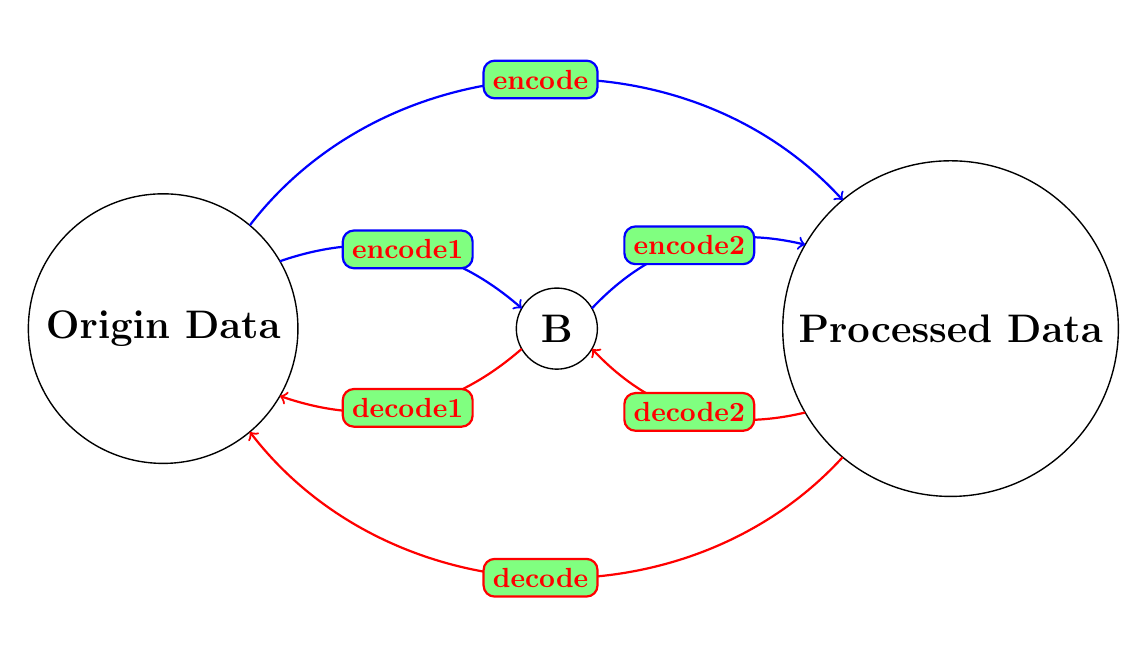
\begin{tikzpicture}
  \SetGraphUnit{5}
  \Vertex{B}
  \WE(B){Origin Data}
  \EA(B){Processed Data}
  \Edge[label = encode1,color = blue](Origin Data)(B)
  \Edge[label = encode2,color = blue](B)(Processed Data)
  \Edge[label = decode2,color = red](Processed Data)(B)
  \Edge[label = decode1,color = red](B)(Origin Data)
  \tikzset{EdgeStyle/.append style = {bend left = 50}}
  \Edge[label = encode,color=blue](Origin Data)(Processed Data)
  \Edge[label = decode,color=red](Processed Data)(Origin Data)
\end{tikzpicture}

\begin{python}
import tensorflow as tf
import matplotlib.pyplot as plt
data_path = '/home/hpc/文档/mnist_tutorial/mnist'

from tensorflow.examples.tutorials.mnist import input_data
mnist = input_data.read_data_sets(data_path, one_hot=False)


# Visualize decoder setting
learning_rate = 0.01
training_epochs = 5
batch_size = 256
display_step = 1
examples_to_show = 10

n_input = 784  # MNIST data input (img shape: 28*28)

x = tf.placeholder(tf.float32,[None,n_input])

n_hidden_1 = 256
n_hidden_2 = 128
weights = {
    'encode_h1':tf.Variable(tf.random_normal([n_input,n_hidden_1])),
    'encode_h2':tf.Variable(tf.random_normal([n_hidden_1,n_hidden_2])),
    'decode_h2':tf.Variable(tf.random_normal([n_hidden_2,n_hidden_1])),
    'decode_h1':tf.Variable(tf.random_normal([n_hidden_1,n_input]))
}
bias = {'encode_h1':tf.Variable(tf.random_normal([n_hidden_1])),
    'encode_h2':tf.Variable(tf.random_normal([n_hidden_2])),
    'decode_h2':tf.Variable(tf.random_normal([n_hidden_1])),
    'decode_h1':tf.Variable(tf.random_normal([n_input]))

}
def encode(x):
    layer_1 = tf.nn.sigmoid(tf.add(tf.matmul(x,weights['encode_h1']),bias['encode_h1']))
    layer_2 = tf.nn.sigmoid(tf.add(tf.matmul(layer_1,weights['encode_h2']),bias['encode_h2']))
    return layer_2

def decode(x):
    layer_1 = tf.nn.sigmoid(tf.add(tf.matmul(x,weights['decode_h2']),bias['decode_h2']))
    layer_2 = tf.nn.sigmoid(tf.add(tf.matmul(layer_1,weights['decode_h1']),bias['decode_h1']))
    return layer_2



encode_op = encode(x)
decode_op = decode(encode_op)
y_pred = decode_op
y_true = x
cost = tf.reduce_mean(tf.square(y_pred-y_true))
optimizer = tf.train.AdamOptimizer(learning_rate).minimize(cost)

with tf.Session() as sess:
    init = tf.global_variables_initializer()
    sess.run(init)
    total_batch = int(mnist.train.num_examples/batch_size)
    for epoch in range(training_epochs):
        for i in range(total_batch):
            batch_xs,batch_ys = mnist.train.next_batch(batch_size)
            _, c = sess.run([optimizer, cost], feed_dict={x: batch_xs})
        if epoch%display_step==0:
            print("Epoch:",'%04d'%(epoch+1),'cost=','{:.9f}'.format(c))
    print('Optimize finish')
    encode_decode = sess.run(y_pred,feed_dict={x:mnist.test.images[:examples_to_show]})
    f,a = plt.subplots(2,10,figsize=(10,2))
    for i in range(examples_to_show):
        a[0][i].imshow(sess.run(tf.reshape(mnist.test.images[i],[28,28])))
        a[1][i].imshow(sess.run(tf.reshape(encode_decode[i],[28,28])))
    plt.savefig('auto_encode.png',dpi=800)
\end{python}
\begin{center}
\begin{figure}[H]
\includegraphics[scale=0.5]{auto_encode.png}
\caption{原图和自编码解码后的图像}
\end{figure}
\end{center}
编码器输出可视化:
\begin{python}
import tensorflow as tf
import matplotlib.pyplot as plt

from tensorflow.examples.tutorials.mnist import input_data
path = '/home/hpc/文档/mnist_tutorial/mnist'
mnist = input_data.read_data_sets(path, one_hot=False)

learning_rate = 0.01
training_epochs = 5
batch_size = 256
display_step = 1
examples_to_show = 10

n_input = 784  # MNIST data input (img shape: 28*28)

X = tf.placeholder("float", [None, n_input])

n_hidden_1 = 256 # 1st layer num features
n_hidden_2 = 128 # 2nd layer num features

learning_rate = 0.01    # 0.01 this learning rate will be better! Tested
training_epochs = 10
batch_size = 256
display_step = 1
n_input = 784  # MNIST data input (img shape: 28*28)
X = tf.placeholder("float", [None, n_input])
n_hidden_1 = 128
n_hidden_2 = 64
n_hidden_3 = 10
n_hidden_4 = 2
weights = {
    'encoder_h1': tf.Variable(tf.truncated_normal([n_input, n_hidden_1],)),
    'encoder_h2': tf.Variable(tf.truncated_normal([n_hidden_1, n_hidden_2],)),
    'encoder_h3': tf.Variable(tf.truncated_normal([n_hidden_2, n_hidden_3],)),
    'encoder_h4': tf.Variable(tf.truncated_normal([n_hidden_3, n_hidden_4],)),
    'decoder_h1': tf.Variable(tf.truncated_normal([n_hidden_4, n_hidden_3],)),
    'decoder_h2': tf.Variable(tf.truncated_normal([n_hidden_3, n_hidden_2],)),
    'decoder_h3': tf.Variable(tf.truncated_normal([n_hidden_2, n_hidden_1],)),
    'decoder_h4': tf.Variable(tf.truncated_normal([n_hidden_1, n_input],)),
}
biases = {
    'encoder_b1': tf.Variable(tf.random_normal([n_hidden_1])),
    'encoder_b2': tf.Variable(tf.random_normal([n_hidden_2])),
    'encoder_b3': tf.Variable(tf.random_normal([n_hidden_3])),
    'encoder_b4': tf.Variable(tf.random_normal([n_hidden_4])),
    'decoder_b1': tf.Variable(tf.random_normal([n_hidden_3])),
    'decoder_b2': tf.Variable(tf.random_normal([n_hidden_2])),
    'decoder_b3': tf.Variable(tf.random_normal([n_hidden_1])),
    'decoder_b4': tf.Variable(tf.random_normal([n_input])),
}
def encoder(x):
    layer_1 = tf.nn.sigmoid(tf.add(tf.matmul(x, weights['encoder_h1']),
                                   biases['encoder_b1']))
    layer_2 = tf.nn.sigmoid(tf.add(tf.matmul(layer_1, weights['encoder_h2']),
                                   biases['encoder_b2']))
    layer_3 = tf.nn.sigmoid(tf.add(tf.matmul(layer_2, weights['encoder_h3']),
                                   biases['encoder_b3']))
    layer_4 = tf.add(tf.matmul(layer_3, weights['encoder_h4']),
                                    biases['encoder_b4'])
    return layer_4
def decoder(x):
    layer_1 = tf.nn.sigmoid(tf.add(tf.matmul(x, weights['decoder_h1']),
                                   biases['decoder_b1']))
    layer_2 = tf.nn.sigmoid(tf.add(tf.matmul(layer_1, weights['decoder_h2']),
                                   biases['decoder_b2']))
    layer_3 = tf.nn.sigmoid(tf.add(tf.matmul(layer_2, weights['decoder_h3']),
                                biases['decoder_b3']))
    layer_4 = tf.nn.sigmoid(tf.add(tf.matmul(layer_3, weights['decoder_h4']),
                                biases['decoder_b4']))
    return layer_4

encoder_op = encoder(X)
decoder_op = decoder(encoder_op)

y_pred = decoder_op
y_true = X

cost = tf.reduce_mean(tf.pow(y_true - y_pred, 2))
optimizer = tf.train.AdamOptimizer(learning_rate).minimize(cost)


with tf.Session() as sess:
    init = tf.global_variables_initializer()
    sess.run(init)
    total_batch = int(mnist.train.num_examples/batch_size)
    for epoch in range(training_epochs):
        for i in range(total_batch):
            batch_xs, batch_ys = mnist.train.next_batch(batch_size)  # max(x) = 1, min(x) = 0
            _, c = sess.run([optimizer, cost], feed_dict={X: batch_xs})
        if epoch % display_step == 0:
            print("Epoch:", '%04d' % (epoch+1),
                  "cost=", "{:.9f}".format(c))
    print("Optimization Finished!")
    encode_decode = sess.run(
        y_pred, feed_dict={X: mnist.test.images[:examples_to_show]})
    encoder_result = sess.run(encoder_op, feed_dict={X: mnist.test.images})
    plt.scatter(encoder_result[:, 0], encoder_result[:, 1], c=mnist.test.labels)
    plt.title('encode output')
    plt.colorbar()
    plt.savefig('auto_encode_v.png',dpi=800)
\end{python}

\begin{center}
\begin{figure}[H]
\includegraphics[scale=0.7]{auto_encode_v.png}
\end{figure}
\end{center}
\section{稀疏编码}
稀疏编码算法是一种无监督学习方法,它用来寻找一组“超完备”基向量来更高效地表示样本数据。稀疏编码算法的目的就是找到一组基向量 $\mathbf{\phi}_i$ ,使得我们能将输入向量 $\mathbf{x}$ 表示为这些基向量的线性组合:
\begin{align}
\mathbf{x} = \sum_{i=1}^k a_i \mathbf{\phi}_{i} 
\end{align}
虽然形如主成分分析技术(PCA)能使我们方便地找到一组“完备”基向量,但是这里我们想要做的是找到一组“超完备”基向量来表示输入向量 $\mathbf{x}\in\mathbb{R}^n$ (也就是说,k > n)。超完备基的好处是它们能更有效地找出隐含在输入数据内部的结构与模式。然而,对于超完备基来说,系数$a_i$不再由输入向量 $\mathbf{x}$ 唯一确定。因此,在稀疏编码算法中,我们另加了一个评判标准“稀疏性”来解决因超完备而导致的退化(degeneracy)问题。

这里,我们把“稀疏性”定义为:只有很少的几个非零元素或只有很少的几个远大于零的元素。要求系数$a_i$ 是稀疏的意思就是说:对于一组输入向量,我们只想有尽可能少的几个系数远大于零。选择使用具有稀疏性的分量来表示我们的输入数据是有原因的,因为绝大多数的感官数据,比如自然图像,可以被表示成少量基本元素的叠加,在图像中这些基本元素可以是面或者线。同时,比如与初级视觉皮层的类比过程也因此得到了提升。

我们把有 m 个输入向量的稀疏编码代价函数定义为:
\begin{align}
\text{minimize}_{a^{(j)}_i,\mathbf{\phi}_{i}} \sum_{j=1}^{m} \left|\left| \mathbf{x}^{(j)} - \sum_{i=1}^k a^{(j)}_i \mathbf{\phi}_{i}\right|\right|^{2} + \lambda \sum_{i=1}^{k}S(a^{(j)}_i)
\end{align}

此处 S(.) 是一个稀疏代价函数,由它来对远大于零的 $a_i$ 进行“惩罚”。我们可以把稀疏编码目标函式的第一项解释为一个重构项,这一项迫使稀疏编码算法能为输入向量 $\mathbf{x}$ 提供一个高拟合度的线性表达式,而公式第二项即“稀疏惩罚”项,它使 $\mathbf{x}$ 的表达式变得“稀疏”。常量$\lambda$是一个变换量,由它来控制这两项式子的相对重要性。

虽然“稀疏性”的最直接测度标准是 "L0" 范式$(S(a_i) = \mathbf{1}(|a_i|>0))$,但这是不可微分的,而且通常很难进行优化。在实际中,稀疏代价函数 S(.) 的普遍选择是L1 范式代价函数 $S(a_i)=\left|a_i\right|_1$  及对数代价函数 $S(a_i)=\log(1+a_i^2)$ 。

此外,很有可能因为减小 $a_i$ 或增加 $\mathbf{\phi}_i$ 至很大的常量,使得稀疏惩罚变得非常小。为防止此类事件发生,我们将限制 $\left|\left|\mathbf{\phi}\right|\right|^2$ 要小于某常量 C 。包含了限制条件的稀疏编码代价函数的完整形式如下:
\begin{equation}
\text{minimize}_{a_i^{(j)},\phi_i}\Sigma_{j=1}^m\|x^{(j)}-\Sigma_{i=1}^ka_i^{(j)}\phi_i\|^2+\lambda\Sigma_{i=1}^kS(s_i^{(j)})\quad\|\phi_i\|^2\leq C,\forall i=1,\ldots,k
\end{equation}
\subsection{稀疏编码的概率表示}
到目前为止,我们所考虑的稀疏编码,是为了寻找到一个稀疏的、超完备基向量集,来覆盖我们的输入数据空间。现在换一种方式,我们可以从概率的角度出发,将稀疏编码算法当作一种“生成模型”。

我们将自然图像建模问题看成是一种线性叠加,叠加元素包括 k 个独立的源特征 $\mathbf{\phi}_i$ 以及加性噪声 ν :
\begin{align}
\mathbf{x} = \sum_{i=1}^k a_i \mathbf{\phi}_{i} + \nu(\mathbf{x})
\end{align}

我们的目标是找到一组特征基向量 $\mathbf{\phi}$ ,它使得图像的分布函数 $P(\mathbf{x}\mid\mathbf{\phi})$ 尽可能地近似于输入数据的经验分布函数 $P^*(\mathbf{x})$ 。一种实现方式是,最小化 $P^*(\mathbf{x})$ 与 $P(\mathbf{x}\mid\mathbf{\phi})$ 之间的 KL 散度,此 KL 散度表示如下:
\begin{align}
D(P^*(\mathbf{x})||P(\mathbf{x}\mid\mathbf{\phi})) = \int P^*(\mathbf{x}) \log \left(\frac{P^*(\mathbf{x})}{P(\mathbf{x}\mid\mathbf{\phi})}\right)d\mathbf{x}
\end{align}

因为无论我们如何选择 $\mathbf{\phi}$ ,经验分布函数 $P^*(\mathbf{x})$ 都是常量,也就是说我们只需要最大化对数似然函数 $P(\mathbf{x}\mid\mathbf{\phi})$ 。 假设v是具有方差$\sigma^2$的高斯白噪声,则有下式:
\begin{align}
P(\mathbf{x} \mid \mathbf{a}, \mathbf{\phi}) = \frac{1}{Z} \exp\left(- \frac{(\mathbf{x}-\sum^{k}_{i=1} a_i \mathbf{\phi}_{i})^2}{2\sigma^2}\right)
\end{align}

为了确定分布 $P(\mathbf{x}\mid\mathbf{\phi})$ ,我们需要指定先验分布 $P(\mathbf{a})$ 。假定我们的特征变量是独立的,我们就可以将先验概率分解为:
\begin{align}
P(\mathbf{a}) = \prod_{i=1}^{k} P(a_i)
\end{align}

此时,我们将“稀疏”假设加入进来——假设任何一幅图像都是由相对较少的一些源特征组合起来的。因此,我们希望$a_i$的概率分布在零值附近是凸起的,而且峰值很高。一个方便的参数化先验分布就是:
\begin{align}
P(a_i) = \frac{1}{Z}\exp(-\beta S(a_i))
\end{align}

这里$S(a_i)$是决定先验分布的形状的函数。

当定义了 $P(\mathbf{x} \mid \mathbf{a} , \mathbf{\phi})$ 和  $P(\mathbf{a})$ 后,我们就可以写出在由 $\mathbf{\phi}$ 定义的模型之下的数据 $\mathbf{x}$ 的概率分布:
\begin{align}
P(\mathbf{x} \mid \mathbf{\phi}) = \int P(\mathbf{x} \mid \mathbf{a}, \mathbf{\phi}) P(\mathbf{a}) d\mathbf{a}
\end{align}

那么,我们的问题就简化为寻找:
\begin{align}
\mathbf{\phi}^*=\text{argmax}_{\mathbf{\phi}} < \log(P(\mathbf{x} \mid \mathbf{\phi})) >
\end{align}

这里 < . > 表示的是输入数据的期望值。

不幸的是,通过对 $\mathbf{a}$ 的积分计算 $P(\mathbf{x} \mid \mathbf{\phi})$ 通常是难以实现的。虽然如此,我们注意到如果$ P(\mathbf{x} \mid \mathbf{\phi}) $的分布(对于相应的 $\mathbf{a}$ )足够陡峭的话,我们就可以用$ P(\mathbf{x} \mid \mathbf{\phi})$ 的最大值来估算以上积分。估算方法如下:
\begin{align}
\mathbf{\phi}^{*'}=\text{argmax}_{\mathbf{\phi}} < \max_{\mathbf{a}} \log(P(\mathbf{x} \mid \mathbf{\phi})) >
\end{align}

跟之前一样,我们可以通过减小$a_i$或增大 $\mathbf{\phi}$ 来增加概率的估算值(因为$P(a_i)$在零值附近陡升)。因此我们要对特征向量 $\mathbf{\phi}$ 加一个限制以防止这种情况发生。
最后,我们可以定义一种线性生成模型的能量函数,从而将原先的代价函数重新表述为:
\begin{align}
E(x,a|\phi):=&-log(P(x|\phi,\mathbf{a})P(\mathbf{a}))\\
            =&\Sigma_{j=1}^m\|x^{(j)}-\Sigma_{i=1}^k\alpha_i^{(j)}\phi_j\|^2+\lambda\Sigma_{i=1}^{k}S(\alpha_i^{(j)})
\end{align}
其中$\lambda = 2\sigma2\beta$ ,并且关系不大的常量已被隐藏起来。因为最大化对数似然函数等同于最小化能量函数,我们就可以将原先的优化问题重新表述为:
\begin{equation}
\mathbf{\phi}^{*},\mathbf{a}^{*}=\text{argmin}_{\mathbf{\phi},\mathbf{a}} \sum_{j=1}^{m} \left|\left| \mathbf{x}^{(j)} - \sum_{i=1}^k a^{(j)}_i \mathbf{\phi}_{i}\right|\right|^{2} + \lambda \sum_{i=1}^{k}S(a^{(j)}_i) 
\end{equation}
使用概率理论来分析,我们可以发现,选择 L1 惩罚和 $\log(1+a_i^2)$ 惩罚作为函数 S(.) ,分别对应于使用了拉普拉斯概率 $P(a_i) \propto \exp\left(-\beta|a_i|\right)$ 和柯西先验概率 $P(a_i) \propto \frac{\beta}{1+a_i^2}$ 。
\section{PCA}
在多元统计分析中,主成分分析(英语:Principal components analysis,PCA)是一种分析、简化数据集的技术。主成分分析经常用于减少数据集的维数,同时保持数据集中的对方差贡献最大的特征。这是通过保留低阶主成分,忽略高阶主成分做到的。这样低阶成分往往能够保留住数据的最重要方面。但是,这也不是一定的,要视具体应用而定。由于主成分分析依赖所给数据,所以数据的准确性对分析结果影响很大。
主成分分析由卡尔·皮尔逊于1901年发明,用于分析数据及建立数理模型。其方法主要是通过对协方差矩阵进行特征分解,以得出数据的主成分(即特征向量)与它们的权值(即特征值)。PCA是最简单的以特征量分析多元统计分布的方法。其结果可以理解为对原数据中的方差做出解释:哪一个方向上的数据值对方差的影响最大?换而言之,PCA提供了一种降低数据维度的有效办法;如果分析者在原数据中除掉最小的特征值所对应的成分,那么所得的低维度数据必定是最优化的(也即,这样降低维度必定是失去讯息最少的方法)。主成分分析在分析复杂数据时尤为有用,比如人脸识别。
PCA是最简单的以特征量分析多元统计分布的方法。通常情况下,这种运算可以被看作是揭露数据的内部结构,从而更好的解释数据的变量的方法。如果一个多元数据集能够在一个高维数据空间坐标系中被显现出来,那么PCA就能够提供一幅比较低维度的图像,这幅图像即为在讯息最多的点上原对象的一个‘投影’。这样就可以利用少量的主成分使得数据的维度降低了。
PCA跟因子分析密切相关,并且已经有很多混合这两种分析的统计包。而真实要素分析则是假定底层结构,求得微小差异矩阵的特征向量。
\subsection{数学定义}
PCA的数学定义是:一个正交化线性变换,把数据变换到一个新的坐标系统中,使得这一数据的任何投影的第一大方差在第一个坐标(称为第一主成分)上,第二大方差在第二个坐标(第二主成分)上,依次类推。
定义一个$n\times m$的矩阵, $X^T$为去平均值(以平均值为中心移动至原点)的数据,其行为数据样本,列为数据类别(注意,这里定义的是$X^T$ 而不是X)。则X的奇异值分解为$X = W\Sigma V^T$,其中$m\times m$矩阵W是$XX^T$的本征矢量矩阵,$\Sigma$是$m\times n$的非负矩形对角矩阵,V是$m\times n$的$X^TX$的本征矢量矩阵。据此,
\begin{equation}
\begin{aligned}
\mathbf{Y}^T&=\mathbf{X}^{T}\mathbf{W}\\
            &=\mathbf{V}{\Sigma}^{T}\mathbf{W}^{T}\mathbf{W}\\
            &=\mathbf{V}{\Sigma}^{T}
\end{aligned}
\end{equation}
当 $m < n − 1$时,$V$ 在通常情况下不是唯一定义的,而$Y$ 则是唯一定义的。$W$ 是一个正交矩阵,$Y^T$是$X^T$的转置,且$Y^T$的第一列由第一主成分组成,第二列由第二主成分组成,依此类推。
为了得到一种降低数据维度的有效办法,我们可以利用$W_L$把 X 映射到一个只应用前面L个向量的低维空间中去:
\begin{equation}
\mathbf{Y} =\mathbf{W_{L}}^{T}\mathbf{X} ={\Sigma _{L}}\mathbf {V} ^{T}
\end{equation}
其中 ${\Sigma _{L}} =\mathbf{I} _{L\times m}{\Sigma }$且$\mathbf{I} _{L\times m} $为$ L\times m L\times m$的单位矩阵。
X 的单向量矩阵W相当于协方差矩阵的本征矢量 $C=XX^T$,
\begin{equation}
XX^T = W\Sigma\Sigma^TW^T
\end{equation}
在欧几里得空间给定一组点数,第一主成分对应于通过多维空间平均点的一条线,同时保证各个点到这条直线距离的平方和最小。去除掉第一主成分后,用同样的方法得到第二主成分。依此类推。在Σ中的奇异值均为矩阵 $XX^T$的本征值的平方根。每一个本征值都与跟它们相关的方差是成正比的,而且所有本征值的总和等于所有点到它们的多维空间平均点距离的平方和。PCA提供了一种降低维度的有效办法,本质上,它利用正交变换将围绕平均点的点集中尽可能多的变量投影到第一维中去,因此,降低维度必定是失去讯息最少的方法。PCA具有保持子空间拥有最大方差的最优正交变换的特性。然而,当与离散余弦变换相比时,它需要更大的计算需求代价。非线性降维技术相对于PCA来说则需要更高的计算要求。
PCA对变量的缩放很敏感。如果我们只有两个变量,而且它们具有相同的样本方差,并且成正相关,那么PCA将涉及两个变量的主成分的旋转。但是,如果把第一个变量的所有值都乘以100,那么第一主成分就几乎和这个变量一样,另一个变量只提供了很小的贡献,第二主成分也将和第二个原始变量几乎一致。这就意味着当不同的变量代表不同的单位(如温度和质量)时,PCA是一种比较武断的分析方法。但是在Pearson的题为 "On Lines and Planes of Closest Fit to Systems of Points in Space"的原始文件里,是假设在欧几里得空间里不考虑这些。一种使PCA不那么武断的方法是使用变量缩放以得到单位方差。
\section{KL散度}
\begin{equation}
	H_p(q)=\sum_{x}q(x)log_2(\frac{1}{p(x)})
\end{equation}
\begin{figure}[H]
	\centering
	\includegraphics[scale=0.4]{CrossEntropyDef.png}
	\caption{Cross\_Entropy\_exp}
\end{figure}
如果按照分别按照$p(x)$和$q(x)$出现的概率计算:
\begin{itemize}
\item $H(p)=\frac{1}{2}\times 1+\frac{1}{4}\times 2+\frac{1}{8}\times 3+\frac{1}{8}\times 3=1.75bit$
\item $H_p(q)=\frac{1}{8}\times 1+\frac{1}{2}\times 2+\frac{1}{4}\times 3+\frac{1}{8}\times 3=2.25bit$
\item $H(q)=\frac{1}{8}\times 3+\frac{1}{2}\times 1+\frac{1}{4}\times 2+\frac{1}{8}\times 3= 1.75bit$
\item $H_q(p)=\frac{1}{2}\times 3+\frac{1}{4}\times 1+\frac{1}{8}\times 2+\frac{1}{8}\times 3 = 2.375bit$
\end{itemize}
将上面的四种情况用图画出来,如果两组概率服从统一分布,他们将相邻:
\begin{figure}[H]
	\centering
	\includegraphics[scale=0.5]{CrossEntropyCompare.png}
	\caption{比较四种情况算得的信息bit}
\end{figure}
上图可以看出$H_p(q)\neq H_q(p)$,为什么?$H_q(p)$更大,因为蓝色被分配了更多的bit,交叉熵给我们了一种方法来衡量两个概率分布的不同。p和q越多不同,p和q对应的交叉熵比p的熵就越大。
\begin{figure}[H]
	\centering
	\includegraphics[scale=0.9]{CrossEntropyQP.png}
	\caption{p对q的交叉熵和p的熵}
\end{figure}
类似的,p和q的差别越大,相应的q对p的交叉熵比q的熵越大。
\begin{figure}[H]
		\centering
			\includegraphics[scale=0.9]{CrossEntropyPQ.png}
				\caption{q对p的交叉熵和q的熵}
\end{figure}
\subsection{交叉熵}
\begin{equation}
	D_p(Q)=H_q(p)-H(p)=\sum_x p(x)log_2(\frac{p(x)}{q{x}})
\end{equation}
$log_2(\frac{p(x)}{q(x)})$表示q表示的代码和q表示的代码有多少个bit不同,整个表达式表示两个代码有多少bit不同。
KL divergence实际上相当于两个分布之间的距离。

相对熵(relative entropy)又称为KL散度(Kullback-Leibler divergence,简称KLD),信息散度(information divergence),信息增益
(information fain)
KL散度是两个概率分布P和Q差别的非对称性度量。KL散度是用来度量基于Q的编码来编码来自P的样本平均所需的额外的位元数。典型情况下,P表示数据的真实分布,Q表示数据的理论分布,模型分布或P的近似分布。

对于离散随机变量,其概率分布P和Q的KL散度可以按下面定义为
\begin{equation}
D_{KL}(P||Q)=\Sigma_iP(i)ln\frac{P(i)}{Q(i)}
\end{equation}
即按概率P求得的P和Q的对数差的平均值。KL散度仅当P和Q各自总和均为1,且对任何t皆满足对于$Q(i)>0$及$P(i)>0$时才有定义。式子出现$oln0$其值按0处理,对于连续随机变量,其概率分布P和Q可按计分方式定义为:
\begin{equation}
D_{KL}(P||Q)=\int_{-\infty}^{\infty}p(x)ln\frac{p(x)}{q(x)}dx
\end{equation}
其中p和q分别表示分布$P$和$Q$的概率密度。
\subsection{相对熵}
由Gibbs不等式可知,当且仅当$P=Q$时$D_{KL}(P||Q)$为0。尽管从直觉上KL散度是个度量或距离函数,但是它实际上
不是一个真正的度量或距离。因为KL散度不具有对称性:从分布P到Q的距离(或度量)通常并不等于从Q到P的距离
(或度量)。
\[D_{KL}(P||Q)\neq D_{KL}(Q||P)\]
自信息和散度的关系:$I(m)=D_{KL}(\delta_{im}||{p_i})$。
互信息和散度:
\begin{align*}
I(X;Y)=&D_{KL}(P(X,Y)||P(X)P(Y))\\
      =&E_x{D_{KL}(P(Y|X)||P(Y))}\\
      =&E_y{D_{KL}P(X|Y)||P(X)}
\end{align*}
信息熵和散度:
\begin{align*}
H(X)&=(i)E_x{I(x)}\\
    &=(ii)logN-D_{KL}(P(X)||P_U(X))
\end{align*}
条件熵和散度:
\begin{align*}
H(X|Y)=&logN-D_{KL}(P(X,Y)||P_U(X)P(Y))\\
      =&(i)logN-D_{KL}(P(X,Y)||P(X)P(Y))-D_{KL}(P(X)||P_U(X))\\
      =&H(x)-I(X;Y)\\
      =&(ii)logN-E_Y{D_{KL}(P(X|Y)||P_U(X))} 
\end{align*}
交叉熵与散度:$H(p,q)=E_p[-logq]=H(p)+D_{KL}(p||q)$
\section{奇异值分解}
我们希望将矩阵分解为矩阵乘的结果:$A_{m\times n}=U_{m\times m}\Sigma_{m\times n} V_{n\times n}^T$,
$\Sigma$矩阵中的对角值被称为原始矩阵$A_{m\times n}$的奇异值。$U_{m\times m}$矩阵的列被称为$A_{m\times m}$的左奇异向量,$V^T_{n\times n}$的矩阵的转置,V的列成为$A_{m\times n}$的右奇异向量。
\begin{python}
from numpy import array
from scipy.linalg import svd
A = array([[1,2],[3,4],[5,6]])
print(A)
U,s,V = svd(A)
\end{python}
生成的s是一个数组,不是矩阵。
\begin{python}
from numpy import array
from numpy import diag
from numpy import dot
from numpy import zeros
from scipy.linalg import svd
A = array([[1,2],[3,4],[5,6]])
U,s,V = svd(A)
Sigma = zeros((A.shape[0],A.shape[1])
B = U.dot(Sigma.fot(V))
print(B)
\end{python}
上面的$\Sigma$对角矩阵的复杂之处仅在于m和n不相等的情况中。当重建一个方形矩阵时,其对角矩阵可以直接使用:
\begin{python}
from numpy import array,diag,dot
from scipy.linalg import svd
A = array([[1,2,3],[4,5,6],[7,8,9]])
print(A)
U,s,V = svd(A)
Sigma = diag(s)
B = U.dot(Sigma.dot(V))
print(B)
\end{python}
\subsection{伪逆}
伪逆是将方形矩阵求逆泛化应用到行列不相等的矩阵上。这也被成为广义的逆(Generalized Inverse)或者(Moore-Penrose Inverse)
。矩阵求逆不是为非方形矩阵定义的。当A的列数大于行数时,那么使用伪逆求解线性方程是众多解决方案中的一种。为你藐视为$S^{+}$,其中A是被求逆的矩阵,+是上标。伪逆是使用A的奇异值分解计算的:
\[A^{+}=VD^+U^T\]这里$A^{+}$是A的伪逆,$D^+$是对角矩阵的伪逆,$U^T$是U的转置。我可可以根据SVD运算得到U和V。$A=U\Sigma V^T$根据$\Sigma$创建一个对角矩阵,计算$\Sigma$中每个非零元素的倒数,然后如果原始矩阵是矩阵的就取其转置,就可以计算得到$D^+$,numpy提供函数pinv()计算举行矩阵的伪逆,下面展示定义了一个$4\times2$的矩阵并定义了其伪逆。
\begin{python}
from numpy import array
from numpy.linalg import pinv
A = array([[0.1,0.2],[0.3,0.4],[0.5,0.6],[0.7,0.8]])
print(A)
B = pinv(A)
print(B)
\end{python}
B为计算出的伪逆。通过人工方式计算伪逆,并将结果和pinv()函数的结果进行比较。首先我们必须计算SVD。然后我们必须计算s数组中每个值的倒数。然后将这个s数据转换成一个对角矩阵,它额外增加一行0以使其变成矩阵形式。最后我们可以根据这些元素计算伪逆。具体实现方式为:
$A^+=V^TD^TU^V$
下面列出完整的实例。
\begin{python}
from numpy import array
from numpy.linalg import svd
from numpy import zeros
from numpy import diag
A = array([[0.1,0.2],[0.3,0.4],[0.5,0.6],[0.7,0.8]])
print(A)
U,s,V = svd(A)
d = 1.0 /s
D = zeros(A.shape)
D[:A.shape[1],:A.shape[1]] = diag(d)
B = V.TDot(D.T).dot(U.T)
print(B)
\end{python}
\subsection{SVD用于降维}
SVD的一大常见应用是降维。具有大量特征的数据(比如特征数(列数)多余观察数(行数)也许可以被规约成所涉及预测问题最相关的更小特征子集。其结果是一个rank更低的接近原是矩阵的矩阵)为了做到这一点,我们可以在原来的数据上执行一次SVD操作并选择$\Sigma$中前k个最大的奇异值。这些列可以从$\Sigma$中选择得到,行可以从$V^T$中选择得到,然后可以重建原始向量A的近似B。
\[B=U.\Sigma_kV^T_k\]
在自然语言处理中,这种方法可以被用在文档中词出现情况或词频的矩阵上,并被称为隐含语义分析(Latent Semantic Analysis)或隐含语义索引(Latent Semantic Indexing)。 此外这种变换可以在原来的矩阵A上计算和应用,也可以在其他类似的矩阵上计算和应用。
\[T=V^TkA\]
下面的示例是使用SVD的数据规约,首先定义一个$3\times10$的矩阵,其列数多余行数。然后计算SVD并且只去前两个特征。这些元素再重新结合起来,得到原是矩阵的准确在线。最后计算转换的方式有两种。
\begin{python}
from numpy import array
from numpy import diag
from numpy import zeros
from scipy.linalg import svd
# define a matrix
A = array([
	[1,2,3,4,5,6,7,8,9,10],
	[11,12,13,14,15,16,17,18,19,20],
	[21,22,23,24,25,26,27,28,29,30]])
print(A)
# Singular-value decomposition
U, s, V = svd(A)
# create m x n Sigma matrix
Sigma = zeros((A.shape[0], A.shape[1]))
# populate Sigma with n x n diagonal matrix
Sigma[:A.shape[0], :A.shape[0]] = diag(s)
# select
n_elements = 2
Sigma = Sigma[:, :n_elements]
V = V[:n_elements, :]
# reconstruct
B = U.dot(Sigma.dot(V))
print(B)
# transform
T = U.dot(Sigma)
print(T)
T = A.dot(V.T)
print(T)
\end{python}

运行这个示例,首先显示定义的矩阵,然后是重建的近似矩阵,然后是原始矩阵的两个同样的变换结果。
scikit-learn 提供了直接实现这种功能的 TruncatedSVD 类。 

TruncatedSVD 的创建必须指定所需的特征数或所要选择的成分数,比如 2。一旦创建完成,你就可以通过调用 fit() 函数来拟合该变换(比如:计算 $V^Tk$),然后再通过调用 transform() 函数将其应用于原始矩阵。结果得到上面被称为 T 的 A 的变换。
下面演示TruncatedSVD类。
\begin{python}

from numpy import array
from sklearn.decomposition import TruncatedSVD
# define array
A = array([
	[1,2,3,4,5,6,7,8,9,10],
	[11,12,13,14,15,16,17,18,19,20],
	[21,22,23,24,25,26,27,28,29,30]])
print(A)
# svd
svd = TruncatedSVD(n_components=2)
svd.fit(A)
result = svd.transform(A)
print(result)
\end{python}
下面的示例演示了 TruncatedSVD 类
运行这个示例,首先显示定义的矩阵,然后是该矩阵变换后的版本。

可以看到,结果得到的值与上面人工计算的结果一致,但某些值的符号不一样。由于所涉及的计算的性质以及所用的基础库和方法的差异,可以预见在符号方面会存在一些不稳定性。只要对该变换进行训练以便复用,这种不稳定性在实践中应该不成问题。

\chapter{Tensorflow基础}
\section{Estimators}
这篇文章介绍简化机器学习程序的高级TensorFlow API\href{https://www.tensorflow.org/api_docs/python/tf/estimator?hl=zh-cn}{ Estimators }。Estimator封装下面的行为:
\begin{itemize}
\item training
\item evaluation
\item prediction
\item export for serving
\end{itemize}
你既可以用我们提供的预先定义好的Estimator也可以写你自己的自定义的Estimator。所有的自定义的或预先提供的Estimators都基于\href{https://www.tensorflow.org/api_docs/python/tf/estimator/Estimator?hl=zh-cn}{tf.estimator.Estimator}类。
\begin{quote}
注意:TensorFlow在\href{https://www.tensorflow.org/api_docs/python/tf/contrib/learn/Estimator?hl=zh-cn}{tf.contrib.learn.Estimator }包含一个你不应该使用的废弃的Estimator。
\end{quote}
\subsection{高级Estimator}
Estimators提供下面的好处:
\begin{itemize}
\item 你可以不用改变你的模型在本地主机或者多服务器环境下运行Estimator-based。更进一步,你可以在CPU,GPU或者没有记录你的模型的TPU运行Estimator-base的模型
\item Estimators简化了模型开发者回见的共同实现
\item 你可以用高级直接代码开发一个艺术模型的状态,简单来讲,通常用Estimator创建模型比TensorFlow低级API要更简单。
\item Estimators本身构建在简化自定义的tf.layers中
\item Estimators为你构建一个图。换句话说,你不用构件图
\item Estimator提供了一个安全的分布式的训练循环控制如何或者什么时候做:
\begin{itemize}
\item 构建图
\item 初始化变量
\item 开始队列
\item 处理异常
\item 创建checkpoint文件并且从失败中恢复
\item 为TensorBoard保存总结文件
\end{itemize}
\end{itemize}
当用Estimator写一个应用时,你必须从模型中分开输入pipeline。分开简化了在不同数据集上的试验。
\subsection{自定义的Estimator}
自定义的Estimator使得你能在高于TensorFlow APIs的高级概念级别上工作。你不用担心创建计算图和会话因为Estimator为你处理所有的plubmbing。预定义的Estimator为你创建管理\href{https://www.tensorflow.org/api_docs/python/tf/Graph?hl=zh-cn}{图}和\href{https://www.tensorflow.org/api_docs/python/tf/Session?hl=zh-cn}{会话}对象。进一步,预定义的Estimators让你做最小的代码改动结合不同的模型架构试验。\href{https://www.tensorflow.org/api_docs/python/tf/estimator/DNNClassifier?hl=zh-cn}{DNNClassfier},例如一个自定义的Estimators类通过dense,前馈神经网络训练分类模型。
\subsection{预定义的Estimator程序结构}
一个预先定义的Estimator的TensorFlow程序通常由四步组成:
\begin{enumerate}
\item 写一个或者更多的数据集导入函数。例如也许创建一个函数导入训练集创建另一个函数导入测试集。每个数据集导入函数必须有两个对象:
\begin{itemize}
\item 一个包含对应特征数据的key为特征名字的value是Tensor的词典
\item 一个Tensor包含一个或者更多标签\newline
例如,下面的代码吧、描述了基本的输入函数框架:
\begin{lstlisting}[language=Python]
def input_fn(dataset):
   ...  # manipulate dataset, extracting feature names and the label
   return feature_dict, label
\end{lstlisting}
(查看\href{https://www.tensorflow.org/programmers_guide/datasets?hl=zh-cn}{Importing Data}获取详细信息)
\end{itemize}
\item 定义特征列。每个\href{https://www.tensorflow.org/api_docs/python/tf/feature_column?hl=zh-cn}{tf.feature\_column}确定特征名字,它的类型和输入预处理。例如,下面的的代码创建三个包含整数和浮点数据的特征列。三个特征列也制定一个lambda程序调用原始数据的缩放:\newline
\begin{lstlisting}[language=Python]
# Define three numeric feature columns.
population = tf.feature_column.numeric_column('population')
crime_rate = tf.feature_column.numeric_column('crime_rate')
median_education = tf.feature_column.numeric_column('median_education',
                    normalizer_fn='lambda x: x - global_education_mean')
\end{lstlisting}
\item 实例化相关的预定义Estimator。例如有一个预先定义的名字为LinearClassfier 的Estimator实现:
\begin{lstlisting}[language=Python]
# Instantiate an estimator, passing the feature columns.
estimator = tf.estimator.Estimator.LinearClassifier(
    feature_columns=[population, crime_rate, median_education],
    )
\end{lstlisting}

\item 调用一个训练,评估,推理方法。例如,所有的Estimator提供一个训练方法训练模型。\newline
\begin{lstlisting}[language=Python]
# my_training_set is the function created in Step 1
estimator.train(input_fn=my_training_set, steps=2000)
\end{lstlisting}
\end{enumerate}
\subsection{预定义Estimators的好处}
预定义的Estimators编码最佳实践提供下面的好处:
\begin{itemize}
\item 最佳决定不同计算图的不同部分应该运行在单台机器或者集群上实现方案的实践
\item 最佳事件(总结)和普遍的有用的总结时间
\end{itemize}
如果你不用自定义的Estimator,你自己必须实现上面的特征。
\subsection{自定义Estimators}
每个Estimator(预定义或者是自定义)的核心是模型函数,它包含了构建训练,评估,预测图的方法。然后当你使用一个预定义的Estimator有些人已经实现了模型函数,当依赖一个自定义的Estimator时,你必须自己写模型函数。一个\href{https://www.tensorflow.org/extend/estimators?hl=zh-cn}{ companion document }解释如何写一个模型函数。
\subsection{推荐的工作流程}
推荐的工作流程如下:
\begin{enumerate}
\item 假设存在一个合适的预定义的Estimator,用它构建你的第一个模型,用它的结果建立一个baseline
\item 构建测试你的pipeline,包含使用这个预定义的Estimator的关于你的数据的完整性和真实性
\item 如果合适的Estimator可用,运行试验决定哪个pre-made Estimator产生最好的结果
\item 可能的话,进一步提高你的模型构建你自定义的Estimator
\end{enumerate}
\subsection{从Keras模型创建Estimator}
你可以转化已经存在的Keras模型为Estimator。这样做能使得你的Keras模型获得Estimator‘s的力量,想分布式的训练。如下面样例调用\href{https://www.tensorflow.org/api_docs/python/tf/keras/estimator/model_to_estimator?hl=zh-cn}{ tf.keras.estimator.model\_to\_estimator}
\begin{lstlisting}[language=Python]
# Instantiate a Keras inception v3 model.
keras_inception_v3 = tf.keras.applications.inception_v3.InceptionV3(weights=None)
# Compile model with the optimizer, loss, and metrics you'd like to train with.
keras_inception_v3.compile(optimizer=tf.keras.optimizers.SGD(lr=0.0001, momentum=0.9),
                          loss='categorical_crossentropy',
                          metric='accuracy')
# Create an Estimator from the compiled Keras model.
est_inception_v3 = tf.keras.estimator.model_to_estimator(keras_model=keras_inception_v3)
# Treat the derived Estimator as you would any other Estimator. For example,
# the following derived Estimator calls the train method:
est_inception_v3.train(input_fn=my_training_set, steps=2000)
\end{lstlisting}
更多细节查看\href{https://www.tensorflow.org/api_docs/python/tf/keras/estimator/model_to_estimator?hl=zh-cn}{tf.keras.estimator.model\_to\_estimator }。
\section{Tensor}
Tensorflow正如它的名字表达的一样是定义tensor的计算。一个tensor是一个概括的矩阵和向量,并且有能力表示更高的维度,我们写Tensorflow程序,主要的对象就是tf.Tensor,一个tensor定义计算的一部分,最后生成值。TensorFlow程序首先用tensor建立一个图,然后运行图获得想要的数据。一个tensor需要指定两个参数:数据类型和形状。Tensor中的数据类型相同,而且总是可知的,形状可能仅仅部分知道。
下面是一些特殊的Tensor类型:
\begin{itemize}
\item	tf.Variable
\item	tf.Constant
\item	tf.Placeholder
\item	tf.SparseTensor
\end{itemize}
\subsection{Rank}
tf.Tensor的rank是对象的维度。TensorFlow的rank和数学中矩阵的rank不一样,下面显示TensorFlow rank和相对应的数学实体
\begin{center}
\begin{tabular}{|c|c|}
\hline
rank&数学实体\\
\hline
0&Scalar(只有值)\\
\hline
1&Vecor(值和方向)\\
\hline
2&矩阵(数值表)\\
\hline
3&3-Tensor\\
\hline
n&n-Tensor\\
\hline
\end{tabular}
\end{center}
\textbf{Rank0}

下面片段展示创建一些0维的变量。
\begin{lstlisting}[language=Python]
mammal = tf.Variable("Elephant", tf.string)
ignition = tf.Variable(451, tf.int16)
floating = tf.Variable(3.14159265359, tf.float64)
its_complicated = tf.Variable((12.3, -4.85), tf.complex64)
\end{lstlisting}
\textbf{Rank1}
传递列表作为初始值创建1维tf.Tensor对象
\begin{lstlisting}[language=Python]
mystr = tf.Variable(["Hello"], tf.string)
cool_numbers  = tf.Variable([3.14159, 2.71828], tf.float32)
first_primes = tf.Variable([2, 3, 5, 7, 11], tf.int32)
its_very_complicated = tf.Variable([(12.3, -4.85), (7.5, -6.23)], tf.complex64)
\end{lstlisting}
\textbf{更高的rank:}
二维的Tensor至少有一行一列
\begin{lstlisting}[language=Python]
mymat = tf.Variable([[7],[11]], tf.int16)
myxor = tf.Variable([[False, True],[True, False]], tf.bool)
linear_squares = tf.Variable([[4], [9], [16], [25]], tf.int32)
squarish_squares = tf.Variable([ [4, 9], [16, 25] ], tf.int32)
rank_of_squares = tf.rank(squarish_squares)
mymatC = tf.Variable([[7],[11]], tf.int32)
\end{lstlisting}
更高rank的Tensor,有n维数组。例如在图像处理,一些tensor的rank为4,维度通常是example-in-batch,image width,image height,color chennel。
\begin{lstlisting}[language=Python]
my_image = tf.zeros([10, 299, 299, 3])  # batch x height x width x color
\end{lstlisting}
\subsection{获取Tensor对象的rank}
你可以使用tf.rank方法获取tensor对象的rank。例如下面获取my3d的rank。
\begin{lstlisting}[language=Python]
r = tf.rank(my3d)	#在图运行后,r将保持值3。
\end{lstlisting}
\subsection{Tensor的切片}
因为tf.Tensor是n维cell阵列,为了访问tf.Tensor的单个cell,你需要指定索引。
对于rank为0的tensor,不需要索引,因为它已经是单个值了。\par
对于rank1(向量),传递一个索引允许你访问:
\begin{lstlisting}[language=Python]
my_scale = my_vector[2]
\end{lstlisting}
如果你想动态的选择向量中的元素,你可以指定[]获取一个tf.Tensor。
传递一个数值访问矩阵的子向量:
\begin{lstlisting}[language=Python]
my_row_vetor = my_matrix[2]
my_column_vector = my_matrix[:, 3]
\end{lstlisting}
\subsection{形状}
shape是tensor每一维元素的个数。TensorFlow在构造图的时候自动计算形状。有时候自动计算可能不知道rank,如果rank已经知道,每一维的形状可能知道可能不知道。
\begin{table}[H]\label{tb:pro1}
\centering
\begin{tabular}{|c|c|c|c|}
\hline
rank&shape&维数&example\\
\hline
0&[ ]&0-D&O维Tensor,标量\\
\hline
1&[D0]&1-D&一维tensor的形状\\
\hline
2&[D0,D1]&2-D&二维Tensoe的形状\\
\hline
3&[D0,D1,D2]&3-D&三维Tensor的形状\\
\hline
n&[D0,D1,\ldots,$D_{n-1}$]&N维tensor的形状[$D_0,D_1,\ldots,D_{n-1}$]&\\
\hline
\end{tabular}
\end{table}
\subsection{获取tf.Tensor对象的形状}
当建立图的时候tensor的形状已知是很有用的,你可以通过tensor的shape属性得到它的形状。得到完全定义的tf.Tensor的形状可以使用tf.shape操作。这个方法你可以建立一个图操作tensor的形状。

例如,这里显示如何创建一个和给定矩阵列数相同的全零向量。
\begin{lstlisting}[language=Python]
zeros = tf.zeros(tf.shape(my_matrix)[1])
\end{lstlisting}
\subsection{改变Tensor的形状}
tensor的元素个数是所有形状值的乘积。标量的元素形状总是1.因此,因为有相同元素不同形状的tensor,转变它们的形状是很方便的。可以使用tf.reshape.

下面例子展示了如何reshape tensor。
\begin{lstlisting}[language=Python]
rank_three_tensor = tf.ones([3, 4, 5])
matrix = tf.reshape(rank_three_tensor, [6, 10])  # Reshape existing content into
                                                 # a 6x10 matrix
matrixB = tf.reshape(matrix, [3, -1])  #  Reshape existing content into a 3x20
                                       # matrix. -1 tells reshape to calculate
                                       # the size of this dimension.
matrixAlt = tf.reshape(matrixB, [4, 3, -1])  # Reshape existing content into a
                                             #4x3x5 tensor

# Note that the number of elements of the reshaped Tensors has to match the
# original number of elements. Therefore, the following example generates an
# error because no possible value for the last dimension will match the number
# of elements.
yet_another = tf.reshape(matrixAlt, [13, 2, -1])  # ERROR!
\end{lstlisting}
\subsection{数据类型}
tf.Tensor不可能有一个以上的数据类型。然而序列化任意数据结构作为字符串存储在tf.Tensor里是可能的。

可以使用tf.cast转换一种数据类型到另一种。
\begin{lstlisting}[language=Python]
# Cast a constant integer tensor into floating point.
float_tensor = tf.cast(tf.constant([1, 2, 3]), dtype=tf.float32)
\end{lstlisting}
通过Tensor的dtype查看tensor的数据类型。你通过python对象创建tf.Tensor的时候需要指定数据类型。如果你不指定TensorFlow选择一个代表你数据的数据类型。TensorFlow转换Python整数为tf.int32,浮点数为tf.float32。转换数组时TensorFlow用和numpy相同的规则。
\subsection{评价Tensor}
当计算图被创建后你可以通过运行计算tf.Tensor获取指定的值。用Tensor.eval方法简单的计算:
\begin{lstlisting}[language=Python]
sess = tf.Session()
constant = tf.constant([1,2,3])
tensor = constant*constant
print(tensor.eval(session=sess))
\end{lstlisting}
eval方法仅仅当tf.Session()被激活时可用。Tensor.eval然后会得到一个和tensor相同数据类型的numpy数组。有时候没有上下文计算tf.Tensor是不可能的。例如,tensor依赖于Placeholder在提供给Placeholder值之前不能计算。
\begin{lstlisting}[language=Python]
p = tf.placeholder(tf.float32)
t = p + 1.0
t.eval()  # This will fail, since the placeholder did not get a value.
t.eval(feed_dict={p:2.0})  # This will succeed because we're feeding a value
                           # to the placeholder.
\end{lstlisting}
其它的模型结构在计算tf.Tensor时可能很复杂。TensorFlow不能直接计算定义在函数内部的或者控制流结构的tf.Tensor。如果tf.Tensor依赖于队列中的值,计算tf.Tensor仅仅入队的时候工作,负责计算被挂起。当和queue工作的时候,记得在计算任何tf.Tensor之前用tf.train.start\_queue\_runners。
\subsection{打印Tensor}
出于调试目的,你想要打印tf.Tesor的值。tfdbg提供了高级的调制支持。TensorFlow用下面的模板打印tf.Tensor:
\begin{lstlisting}[language=Python]
t = <<some tensorflow operation>>
print(t)  # This will print the symbolic tensor when the graph is being built.
         # This tensor does not have a value in this context.
\end{lstlisting}
这段代码打印tf.Tensor对象不是它的值,TensorFlow提供了tf.Print操作,然后第一个没有改变的Tensor参数然后打印tf.Tensor的第二个参数。

为了正确的使用tf.Print(),必须要用它的返回值,查看下面的例子:
\begin{lstlisting}[language=Python]
	#we are using the value returned by tf.Print
result = t + 1  # Now when result is evaluated the value of `t` will be printed.
\end{lstlisting}
当你计算result你将计算result依赖的每个结果,因为result依赖于t,然后计算t,打印它的输入,t被打印。
\section{Variable}
Tensorflow变量是在你的程序中表现共享,永久状态的最好的方法,Vaiables通过tf.Variable类操作。一个tf.Variable代表随着在它上面的操作的进行它的值可能被改变。
和tf.Tensor不同在于tf.Variable存在于session.run之外。一个tf.Vaiable存储永久tensor,指定操作允许你读和修改它的值,修改能通过多个tf.Session可视化,因此多个worker对于同一个tf.Variable可以查看到同样的值。
\subsection{创建变量}
创建变量最好的方法是调用tf.get\_variable函数。这个函数要求你指定变量的名字,名字将作为副本访问相同的变量,与checkpoint和导入模型时变量的名字一样。tf.get\_variable也允许你重用一个先前创建的有同样名字的变量,使得定义重用层很方便。
创建变量提供名字和形状。
\begin{lstlisting}[language=Python]
	my_variable = tf.get_variable("my_variable",[1,2,3])
\end{lstlisting}
上面代码创建了一个3维tensor变量my\_variable,它的形状为[1,2,3],默认数据类型为tf.float32,通过随机tf.glorot\_uniform\_initializer初始化值。
你也可以指定dtype和初始化方式。
\begin{lstlisting}[language=Python]
	my_variable = tf.get_variable("my_int_variable",[1,2,3],dtype=tf.int32,initializer=tf.zeros_initializer)
\end{lstlisting}
TensorFlow提供很一些方便的初始化器,你也可以通过有值的tf.Tensor初始化一个tf.Variable。
\begin{lstlisting}[language=Python]
	other_variable = tf.get_variable("other_variable",dtype=tf.int32,initializer=tf.constant([23,42]))
\end{lstlisting}
所以当你用tf.Tensor作为初始化器你不要指定变量的形状,因为初始化器用你的Tensor的形状。
\subsection{变量集合}
因为断开一部分TensorFlow程序也许是想创建变量,这有时候是一个简单的访问它们的方法。因此TensorFlow提供了collections(集合)代表有名字的tensor列表或者其它对象,像tf.Variable实体。

默认每个tf.Variable被放在下面的两个collections:tf.Graphkeys.Global\_VARIABLE(可以被多个设备共享的变量),tf.Graphkeys.TRAINABLE\_VARIABLE(TensorFlow将计算梯度的变量)。如果你不想一个变量被训练,将它增加到tf.GraphKeys.LOCAL\_VARIABLE集合。例如下面的代码段展示了如何增加一个my\_local变量到这个集合。
\begin{lstlisting}[language=Python]
my_local = tf.get_variable("my_local",shape=(),collections=[tf.GraphKeys.LOCAL_VARIABLES])
# TensorFlow1.4后续版本使用
# my_local = tf.get_variable("my_local",shape=(),collections=[tf.GraphKeys.GLOBAL_VARIABLES])
\end{lstlisting}
你也可以指定trainable=False。
\begin{lstlisting}[language=Python]
my_non_trainable = tf.get_variable("my_non_variable",shape=(),trainable=False)
\end{lstlisting}
你也可以用你自己的collections。任何字符串都是一个可用的集合的名字,不需要明确的创建集合。增加一个变量(或者任何对象)到集合后创建变量,调用tf.add\_to\_collection。例如,你可以用下面的代码增加一个已经存在的变量my\_local到一个my\_collection\_name集合:
\begin{lstlisting}[language=Python]
	tf.add_to_collection("my_collection_name",my_local)
\end{lstlisting}
你可以用下面的代码获取你放置在collection里面的变量的和对象列表。
\begin{lstlisting}[language=Python]
tf.get_collection("my_collection_name")
\end{lstlisting}
\subsection{配置设备}
像任何其它TensorFlow操作一样,你可以放置变量到特别的设备上。例如,下面的代码片在第二个GPU上创建一个变量v。
\begin{lstlisting}[language=Python]
with tf.device("gpu:1"):
    v = tf.get_variable("v",1)
\end{lstlisting}
对于变量在正确的设备上部署是很重要的。有时候放变量在worker上而不是参数服务器上,例如可能极大的减缓训练,在最坏的情况下让每个worker独立的复制每个变量。为此我们提供了tf.train.replica\_device\_setter。自动放置变量到参数servers上。例如:
\begin{lstlisting}[language=Python]
cluster_spec={
	"ps":["ps0:2222","ps1:2222"],
	"worker":["worker0:2222","woker1:2222","worker2:2222"]}
with tf.device(tf.train.replica_device_setter(cluster=cluster_spec)):
    v = tf.get_variable("v",shape=[20,20])#这个变量被replica_device_setter放置在参数server上
\end{lstlisting}
\subsection{初始化变量}
{\color{red}{在使用变量之前,你必须对变量进行初始化。}}如果你在低级的TensorFlow API(明确的创建自己的图和会话)上编程,你必须明确的初始化变量。最高级的框架像tf.contrib.slim,\newline
tf.estimator.Estimator和Keras在你训练模型前自动初始化变量。

明确的初始化是很有用的,因为它让你从checkpoint载入模型不用重复运行代价高昂的初始化器同时允许决定什么时候随机初始化的变量在分布式设置上被共享。

为了在开始训练之前初始化可训练的变量,调用tf\_global\_variables\_initilizer().这个函数是一个初始化tf.GraphKeys.GLOBAL\_VARIABLES集合所有变量的操作。运行下面的操作初始化所有的变量:
\begin{lstlisting}[language=Python]
session.run(tf.global_variable_initializer())
\end{lstlisting}
如果你需要手动初始化变量,你可以运行变量初始化操作:
\begin{lstlisting}[language=Python]
session.run(my_variable.initializer)
\end{lstlisting}
你可以查询那些变量没有被初始化:
\begin{lstlisting}[language=Python]
print(session.run(tf.report_uninitialized_variables()))
\end{lstlisting}
注意,默认情况下tf.global\_variables\_initializer不指定变量的初始化顺序。因此一个初始化值依赖于另一个初始化值时,你可能得到错误。任何时候你在一个不是所有的变量被初始化(用一个变量值的时候另一个变量正在初始化)的环境下最好用variable.initialized\_value()代替variable。
\begin{lstlisting}[language=Python]
v = tf.get_variable("v",shape=(),initializer=tf.zeros_initializer())
w = tf.get_variable("w",initializer=tf.initialized_value()+1)
\end{lstlisting}
\subsection{用变量}
为了在TensorFlow图中使用tf.Variable,简单的把变量当作tf.Tensor。
\begin{lstlisting}[language=Python]
v = tf.get_variable("v",shape=(),initializer=tf.zeros_initializer())
w = v+1    # w是一个基于v的值计算的Tensor,任何时候一个用在表达式中的变量自动转化一个tf.Tensor到它的值。
\end{lstlisting}
赋值给一个变量用方法assign,assign\_add和tf.Variable。例如你可以这样调用这些方法:
\begin{lstlisting}[language=Python]
v = tf.get_variable("v",shape=(),initializer=tf.zeros_initializer)
assignment = v.assign_add(1)
tf.global_variable_initializer().run()
assignment.run()
\end{lstlisting}
多数TensorFlow优化器根据一些类似梯度下降的算法已经指定了高效的更新变量值的操作。因为变量是可以更改的,有时候知道变量任何时间点被使用的值是很有用的。你可以用tf.Variable.read\_value在有时候变量使用后读取变量的值。
\begin{lstlisting}[language=Python]
v = tf.get_variable("v",shape=(),initializer=tf.zeros_initializer())
assignment = v.assign_add(1)
with tf.control_dependencuies([assignment]):
    w = v.read_value()
\end{lstlisting}
\subsection{保存和恢复}
用tf.train.Saver对象保存恢复模型是一种最简单的方法。这个构造器为图上所有的或者指定的变量添加save和restore操作。Saver提供了方法运行这些操作,指定checkpoint文件读写的路径。为了恢复模型的checkpointe而不是图,你必须首先从MetaGraph(.meta扩展的)文件。通过调用tf.train.import\_meta\_graph,从执行一个restore返回一个Saver。
\subsection{checkpoint文件}
TensorFlow保存变量在一个二进制文件中,大体上是映射变量的名字到tensor的值。当你创建一个Saver对象,你可以从checkpoint文件选择变量,默认对每个变量用tf.Variable.name的值。
\subsection{保存变量}
用tf.train.Saver()创建一个Saver管理模型的所有变量。例如,下面的代码段展示了如何调用tf.train.Saver.save()方法保存变量为一个checkpoint文件。
\begin{lstlisting}[language=Python]
# 创建变量
v1 = tf.get_variable("v1",shape=[3],initializer = tf.zeros_initializer)
v2 = tf.get_variable("v2",shape=[5],initializer = tf.zeros_initializer)
inc_v1 = v1.assign(v1+1)
dec_v2 = v2.assign(v2-1)
# 增加一个操作初始化变量
init_op = tf.global_variables_initializer()
# 增加操作保存所有的变量
saver = tf.train.Saver()
# 载入模型初始化变量,保存变量到磁盘
with tf.Session() as sess:
    sess.run(init_op)
    inc_v1.op.run(session = sess)
    dec_v2.op.run(session = sess)
    save_path = saver.save(sess,'./model.ckpt')
    print("Model saved in file:%s"%save_path)
\end{lstlisting}
\subsection{恢复变量}
tf.train.Saver对象不仅可以保存变量到checkpoint文件,也可以恢复变量。注意当你从一个文件恢复变量的时候你没有必要提前初始化它们。例如,下面的代码段展示了如何调用tf.train.Saver.restore方法从checkpoint文件恢复变量。
\begin{lstlisting}[language=Python]
tf.reset_default_graph()
v1 = tf.get_variable("v1",shape=[3])
v2 = tf.get_variable("v2",shape=[5])
saver = tf.train.Saver()
with tf.Session() as sess:
    saver.restore(sess,'./model.ckpt')
    print("模型恢复")
    print("v1:%s"%v1.eval())
    print("v2:%s"%v2.eval())
\end{lstlisting}
\subsection{选择变量恢复}
如果你不传递任何参数给tf.train.Saver(),saver处理图上所有的变量。每个变量按照变量创建的时候给定的名字保存。有时候明确的指定checkpoint文件中的变量的名字是有用的。例如你也许训练一个五层神经网络,你现在想重用之前的五层网络训练一个新的6层网络,你可以用saver恢复前面5层的权重。你可以通过传递给tf.train.Saver()构造体变量列表的名字或者(一个key是名字value是值的)Python字典保存和载入变量。
\begin{lstlisting}[language=Python]
tf.reset_default_graph()
	v1 = tf.get_variable("v1",[3],initializer = tf.zeros_initializer)
	v2 = tf.get_variable("v2",[5],initializer = tf.zeros_initializer)
	saver = tf.train.Saver({"v2:":v2})
	with tf.Session() as sess:
	    v1.initializer.run()
	    saver.restore(sess,"./model.ckpt")
	    print("v1 : %s" % v1.eval())
	    print("v2 : %s" % v2.eval())
\end{lstlisting}
注意
\begin{itemize}
	\item 如果你想保存和恢复模型的变量的子集,你可以创建多个Saver对象,它的值仅仅在Saver.restore()方法运行的时候才被载入。
	\item 如果你仅仅在会话开始时恢复变量的一个子集,你必须对其它变量执行初始化操作。
\end{itemize}
\subsection{共享变量}
TensorFlow支持两种方法的共享变量:
\begin{itemize}
	\item 明确传递tf.Variable()对象
	\item 在tf.variable\_scope对象中隐式打包tf.Variable对象。
\end{itemize}
用Veriable scope允许你控制变量重用调用函数,隐式的创建使用变量。它也允许你在你的文件结构上命名你的变量以方便理解。
\begin{lstlisting}[language=Python]
def conv_relu(input,kernel_shape,bias_shape):
    weights = tf.get_variable("weight",kernel_shape,initializer=tf.random_normal_initializer())
    biases = tf.get_variable("biase",biase_shape,initializer=tf.constant_initializer(0.0))
    conv = tf.nn.conv2d(input,weights,striders=[1,1,1,1],padding="SAME")
    return tf.nn.relu(conv+biases)
\end{lstlisting}
这个函数用weights和biases好处是清晰。在真实的模型中,我们想要一些卷基层,重复的调用这些函数将not work:
\begin{lstlisting}[language=Python]
input1 = tf.random_normal([1,10,10,32])
input2 = tf.random_normal([1,20,20,32])
x = conv_relu(input1,kernel_shape=[5,5,1,32],bias_shape=[32])
x = conv_relu(x,kernel_shape=[5,5,32,32],bias_shape=[32])
\end{lstlisting}
因为希望的行为不确定(创建新的变量还是重用之前的变量?)TensorFlow将不能做到。在不同的scope调用conv\_relu,并且我们想创建新的变量:
\begin{lstlisting}[language=Python]
def my_image_filter(input_images):
    with tf.variable_scope("conv1"):
    #这里被创建的变量名字为"conv1/weights","conv1/biases"
        relu1 = conv_relu(input_images,[5,5,1,32],[32])
    with tf.variable_scope("conv2"):
	return conv_relu(relu1,[5,5,32,32],[32])
\end{lstlisting}
如果你想你的变量被共享,你有两个字选择。第一,你可以在创建一个scope的时候用resue=True:
\begin{lstlisting}[language=Python]
with tf.variable_scope("model"):
    output1 = my_image_filter(input1)
with tf.variable_scope("model",reuse=True):
    output2 = my_image_filter(input2)
\end{lstlisting}
你可以调用scope.resue\_variable()触发一个reuse:
\begin{lstlisting}[language=Python]
with tf.variable_scope("model") as scope:
    output1 = my_image_filter(input)
    scope.reuse_variables()
    output2 = my_image_filter(input2)
\end{lstlisting}
因为用来提取scope名字提取字符串可能很危险,也可以用下面的方法初始化:
\begin{lstlisting}[language=Python]
with tf.variable_scope("model") as scope:
    output1 = my_image_filter(input1)
with tf.variable_scope(scope,reuse=True):
    output2 = my_image_filter(input2)
\end{lstlisting}
\section{图(Graphs)和会话(Session)}
TensorFlow用数据流图(dataflow graph)代表操作间的相应的计算。这导致首先你需要先定义图,创建TensorFlow Session通过本地设备或远程设备运行图的一部分。这个向导对于你想用低级变量模型是很有用的。要记得像tf.estimator.Estimator和Keras中的API对于用户端隐藏了图和会话的细节。
\subsection{为什么用数据流图?}
数据流图对于并行编程来说是一个常见的模型。在数据流图中,节点(node)代表了计算单元,边(edge)代表了数据消耗和产生。例如在TensorFlow图中,tf.matmul操作将对应两个边(两个相乘的矩阵)单个节点一个输出(相乘的结果)。
TensorFlow利用数据流图计算有如下好处:
\begin{itemize}
\item 并行性:通过指定边代表不同操作间的依赖,系统能很容易的识别能并行执行的操作。
\item 分布执行:通过用边代表值在不同操作间的流动,这对于tensorflow分割你的程序到不同的机器上的设备(CPUs,GPUs,TPUs)上,TensorFlow插入必须的计算和不同设备间的协调。
\item 编译:TensorFlow的XLA compiler可以用你的数据流图的信息生成更快的代码,例如通过融合连接操作。
\item 数据流图是一个代表你模型的代码,你可以用Python建立图,存储在SavedModel,为了更低的推理延迟在C++程序中恢复。
\end{itemize}
\subsection{建立一个tf.Graph}
大多数的TensorFlow的开始阶段构造一个数据流图,在这个阶段,你利用TensorFlow的API函数构造tf.Operation(节点)和tf.Tensor(边)对象,添加它们到图实例上。TensorFlow提供默认的图到相同上下文环境下的API函数,例如:
\begin{itemize}
\item 调用tf.constant(42.0)创建一个tf.Operation生成值42.0,添加值到默认的图上,返回一个代表这个常量值的tf.Tensor。
\item 调用tf.matmul(x,y)创建一个tf.Tensor对象x,y用tf.Operation相乘,增加它到默认的图上,返回一个代表相乘结果的tf.Tensor。
\item 执行 v=tf.Variable(0)给图添加一个tf.Operation到图上,操作将在tf.Session.run调用前存储可以写的Tensor值。tf.Variable对象包装这个操作,然后它能被像tensor一样使用,Tensor将读取当前存储的值。tf.Variable对象有assign和assign\_add之类的方法,当方法被执行的时候,更新存储的值。
\item 调用tf.train.Optimizer.minimize将操作和tensor添加到默认的图上计算梯度,返回一个tf.Operation,当运行的时候,用图读设置变量。
\end{itemize}
多数程序依赖于默认的图,在TensorFlow API调用大多数程序仅仅添加操作和tensor到默认的图上,并不执行实际的计算。当你通过这些tf.Tensor和tf.Operation表示你的函数,传递给tf.Session进行计算。
\subsection{命名你的操作}
tf.Graph对象给它包含的tf.Operation对象定义了一个namespace。TensorFlow自动为你图上的操作选择一个独一无二的名字,而且指定操作名字使程序易读和方便调试。TensorFlow API提供了两个操作来覆盖操作的名字:
\begin{itemize}
\item 每个API函数在创建一个新的tf.Operation或者返回一个新的tf.Tensor时接收一个name选项。例如tf.constant(42.0,name="answer")创建一个新的操作名字叫answer,返回一个名字为”answer:0“的tf.Tensor。如果默认图已经包含了名字为"answer"的操作,TensorFlow将添加"-1","-2"等等,例如:
\begin{lstlisting}[language=Python]
c_0 = tf.constant(0,name="c")#操作的名字为"c"
c_1 = tf.constant(2,name="c")#操作的名字为"c_1"
with tf.name_scope("outer"):
    c_2 = tf.constant(2,name="c")#操作的名字为outer/c
    with tf.name_scope("inner"):
        c_2 = tf.constant(3,name="c")
    c_4 = tf.constant(4,name="c")#操作名字为"outer/c_1"
    with tf.name_scope("inner"):
        c_5 = tf.constant(5,name="c")
\end{lstlisting}
\end{itemize}
tf.Tensor对象隐藏为tf.Operation名字,之后tf.Operation将产生tensor作为输出。一个tensor的名字形式"<OP\_NAME>:<i>",这里:
\begin{itemize}
\item "<OP\_NAME>"是产生它的操作的名字。
\item "<i>"是一个整数操作输出的tensor的索引。
\end{itemize}
\subsection{放置操作在不同的设备上}
如果你想TensorFlow用多个不同的设备,tf.device函数提供了方便的方法来在一个特别的上下文中请求所有的操作放置在相同的设备上。
指定格式如下:
\begin{lstlisting}[language=Python]
/job:<JOB_NAME>/task:<TASK_INDEX>/device:<DEVICE_TYPE>:<DEVICE_INDEX>
\end{lstlisting}
这里:
\begin{itemize}
\item <JOB\_NAME>是一个alpha数字,不是以数字开头
\item <DEVICE\_TYPE>是一个注册的设备。
\item <TASK\_INDEX>一个非负整数代表job中的任务的索引
\item <JOB\_NAME>查看tf.train.ClusterSpec查看更多关于jobs和tasks的解释。
\item <DEVICE\_INDEX>:一个代表device索引的非负整数,例如为了区别在同一进程中的不同GPU。
\end{itemize}
你不需要指定设备的每一部分,例如,如果你运行在一个单GPU的机器上,你也许用tf.device添加一些操作到CPU和GPU上。
\begin{lstlisting}[language=Python]
weights = tf.random_normal()
with tf.device("/device:CPU:0")
    img = tf.decode_jpeg(tf.read_file("img.jpg"))
with tf.device("/device:GPU:0"):
    result = tf.matmul(weights,img)
\end{lstlisting}
如果你用典型的分布式配置部署TensorFlow,你也许指定job的名字和task ID放置变量到参数服务器job("/job:ps"),其它的操作到worker job("/job:worker")
\begin{lstlisting}[language=Python]
with tf.device("/job:ps/task:0"):
    weight_1 = tf.Variable(tf.truncated_normal([784,100]))
    biases_1 = tf.Variable(tf.zeros([100]))
with tf.device("/job:ps/task:1"):
    weight_2 = tf.Variable("/job:ps/task:1"):
    biases_2 = tf.Variable(tf.zeros([10]))
with tf.device("/job:worker"):
    layer_1 = tf.matmul(train_batch,weight_1)+biases_1
    layer_2 = tf.matmul(train_batch,weight_2)+biases_2
\end{lstlisting}
tf.device给你很高的灵活度度来选择放置单个操作或者更大范围的TensorFlow图。在一些情况下,有简单的算法。例如tf.train.replica\_device\_setter API可以用tf.device放置操作data-parallel distributed training.例如下面的代码段显示tf.train.replica\_device\_setter应用不同的放置策略到tf.Virable对象和其它操作:
\begin{lstlisting}[language=Python]
with tf.device(tf.train.replica_device_setter(ps_tasks=3)):
# tf.Variable objects are, by default, placed on tasks in "/job:ps" in a
# round-robin fashion.
    w_0 = tf.Variable(...)  # placed on "/job:ps/task:0"
    b_0 = tf.Variable(...)  # placed on "/job:ps/task:1"
    w_1 = tf.Variable(...)  # placed on "/job:ps/task:2"
    b_1 = tf.Variable(...)  # placed on "/job:ps/task:0"
    input_data = tf.placeholder(tf.float32)     # placed on "/job:worker"
    layer_0 = tf.matmul(input_data, w_0) + b_0  # placed on "/job:worker"
    layer_1 = tf.matmul(input_data, w_1) + b_1  # placed on "/job:worker"
\end{lstlisting}
\subsection{Tensor-like对象}
一些TensorFlow操作接收一个或者更多的tf.Tensor对象作为参数。例如,tf.matmul得到tf.Tensor对象,tf.add\_n得到一个tf.Tensor列表对象。为了方便使用这些函数在tf.Tensor中接收一个tensor-like对象,用tf.convert\_to\_tensor方法转换它为tf.Tensor,Tensor-like包含下面的元素类型:
\begin{itemize}
\item tf.Tensor
\item tf.Variable
\item numpy.ndarray
\item list(tensor-like对象的列表)
\item Python标量:bool,float,int,str。
\end{itemize}
你可以用tf.register\_tensor\_convension\_function。

默认,每次你的相同的tensor-like对象TensorFlow将创建一个新的tf.Tensor。如果tensor-like对象很大(numpy.ndarray包含一些训练样本),当你多次使用你也许会超出内存。为了避免这样,手动调用tf.convert\_to\_tensor在tensor-like对象,用tf.Tensor返回。
\subsection{在tf.Session执行图}
TensorFlow用tf.session类代表客户程序(通常是Python程序),通过一个类似的接口在(C++也可用),一个tf.Session对象提供访问在本地机器上的设备,远程设备用分布式的TensorFlow域。它也缓存一些关于你的tf.Graph的信息以至于你能高效的运行相同的计算多次。
\subsection{创建tf.Session}
如果你用低层的TensorFlow API,你可以为当前图创建一个tf.Session
\begin{lstlisting}[language=Python]
#创建一个默认的session
with tf.Session() as sess:
#创建一个远程会话
with tf.Session("grpc://example.org:2222"):
\end{lstlisting}
因为一个tf.Session拥有自己的物理资源(像GPU和网络连接),它是通常用作上下文管理(with),自动关闭会话。但是你应该确定调用tf.Session.close在程序结束后释放资源。

高级API像tf.train.MonitoredTrainingSession或者tf.estimator.Estimator将为你创建和管理一个tf.Session。APIs接收target和config参数(或者作为tf.estimator.RunConfig的一部分),含义如下:
tf.Session.\_\_init\_\_接收三个参数:
\begin{itemize}
	\item target 如果这个参数为空,会话仅仅用在本地机器上。然而,你也许指定grpc:// URL指定TensorFlow Server地址,让会话访问server上的所有设备。查看tf.train.Server查看TensorFlow创建server的详细信息。例如通常between-graph replication配置,tf.Session在同一进程中作为客户连接tf.train.Server。
	\item graph 默认情况下新的tf.Session将被限制到仅能在当前的图上运行操作。如果你在你的程序中用多个图,你可以在创建会话的时候指定tf.Graph。
	\item config 这个参数允许你指定tf.Configproto控制session的行为。例如包含一些配置选项。
	\item allow\_soft\_placement 设置设个参数为True使用soft 设备放置算法,该算法忽略tf.device注释,尝试放置CPU-only操作在GPU设备上。
	\item cluster\_def:当用分布式的TensorFlow,这个选项允许你指定用于计算的机器,提供不同job名字的映射任务索引和网络地址。
	\item graph\_option.optimizer\_options:在执行前提供控制优化TensorFlow的执行。
	\item gpu\_options.allow\_grouth:设置为True改变GPU内存分配因至于它的随着内存分配渐渐增长,而不是启动的时候分配尽量多的内存。
\end{itemize}
\subsection{用tf.Session.run执行操作}
tf.Session.run是运行tf.Operation和评估tf.Tensor的主要操作,可以传递一个或者更多的tf.Operation和tf.Tensor或者tensor-like 类型的对象,像tf.Variable。这些fetch决定了tf.Graph的使用与计算fetch的所有子图操作的输出。例如下面的代码片段显示了不同的参数能操作不同的子图执行:
\begin{lstlisting}[language=Python]
x = tf.constant([[37.0,-23.0],[1.0,4.0]])
w = tf.Variable(tf.random_uniform([2,2]))
y = tf.matmul(x,w)
output = tf.nn.softmax(y)
init_op = w.initializer
with tf.Session() as sess:
#初始化变量
    sess.run(init_op)
    print(sess.run(output))
    y_val,output_val = sess.run([y,output])
\end{lstlisting}
tf.Session.run也可以用feeds字典,字典映射tf.Tenor(常见的tf.placeholder())对象为合适执行的值(典型的Python标量,列表,Numpy数组)。
\begin{lstlisting}[language=Python]
x = tf.placeholder(tf.float32,shape=[3])
y = tf.square(x)
with tf.Session() as sess:
    print(sess.run(y,{x:[1.0,2.0,3.0]}))
    print(sess.run(y,{x:[0.0,0.0,5.0]}))
    #sess.run(y) 运行z此代码会Raise  `tf.errors.InvalidArgumentError`
    #因为当你计算一个tensor的时候它以来的值应该给定。
    #sess.run(y,{x:37.0})Raises `ValueError`,因为37.0的形状不匹配
\end{lstlisting}
tf.Session.run也接收一个选项options参数使你指定调用的选项,run\_metadata参数使你收集关于执行的metadata。例如你可以用下面的选项处理执行信息:
\begin{lstlisting}[language=Python]
y = tf.matmul([[37.0,-23.0],[1.0,4.0]],tf.random_uniform([2,2]))
with tf.Session() as sess:
	#定义sess.run的选项
    options = tf.RunOptions()
    options.output_partition_graphs = True
    options.trace_level = tf.RunOptions.FULL_TRACE
#定义返回metadata的容器
metadata = tf.RunMetadata()
sess.run(y,options=options,run_metadata=metdadata)
#打印每个设备执行的子图
print(metadata.partition_graphs)
\end{lstlisting}
\subsection{GraphDef和MetaGraphDef}
TensorFlow用数据流图作为程序的表示,一个tf.Graph包含两个相关的信息:
\begin{itemize}
\item 图的结构(Graph structure):节点和边指示了操作如何被组合在一起。但是没有描述它们如何被使用,图的结构像集合代码,查看它们可能传达一些有用的信息,但是它不包含源代码传送的所有信息。
\item 图集合(Graph collections)TensorFlow提供了一个通常的机制从tf.Graph的恢复metadata集合。tf.add\_to\_collection函数使得你能用key(tf.GraphKeys定义的一些标准的key)结合列表对象,tf.get\_colletion使得你能结合key查看所有的对象,一些TensorFlow库用如下机制:当你创建一个tf.variable,它被增加到代表全局变量和训练的变量集合中,之后你创建一个tf.train.Saver或者tf.train.Optimizer,集合中的变量被用作默认参数。
\end{itemize}
一个图可以用两种形式表示:
\begin{itemize}
	\item tf.GraphDef:合适图结构的低级表示,包含所有操作的描述和它们之间的边。tf.GraphDef代表使用的低级APIs,像tensorflow:session C++ APIs 通常它要求额外的上下文环境(如典型的操作的名字)来充分使用它。tf.Graph.as\_graph\_def方法转换一个tf.Graph为tf.GraphDef。
	\item tf.train.MetaGraphDef:这是数据流图的高级表示它包含一个tf.GraphDef,和一些帮助我们理解图的信息(像图集合的上下文信息)。tf.train.export\_meta\_graph函数转化一个tf.Graph为tf.trainMetaGraphDef。tf.train.Saver.save方法也写一个\newline tf.train.MetaGraphDef,它可能被用在结合保存的checkpoint文件去恢复训练保存点的状态。
\end{itemize}
通常情况下我们鼓励你用tf.train.MetaGraphDef而不是tf.GraphDef。在一些情况下tf.GraphDef是很有用的,例如当用下tf.import\_graph\_def或者Graph Transform这样的低级函数修改图,但是tf.train.MetaGraphDef建议用于高级应用。例如用tf.train.MetaGraphDef SavedModel library包装tf.Graph和一系列训练模型参数以至于它们能被后续服务使用。

如果你有tf.train.MetaGraphDef,tf.train.import\_meta\_graph函数将载入默认的图,调用这个函数有下面两种特征:
\begin{itemize}
	\item 它将从原始的图集合中恢复图的内容。像tf.global\_variable和默认的参数像 \newline tf.train.latest\_checkpoint 函数可能被用于从类似的checkpoint目录寻找最新的checkpoint
\end{itemize}
如果你有一个tf.GraphDef,tf.import\_graph\_def函数使得你能载入图进一个已经存在的python tf.Graph对象。为了利用导入的图,你必须知道在tf.GraphDef中操作或者Tensor的名字。tf.import\_graph\_def函数有两个主要的特性帮你导入的图:
\begin{itemize}
	\item 你可以通过传递选项input\_map参数重新绑定导入图的tensor对象到默认的图。例如,input\_map使你获取定义在tf.GraphDef导入图的片段,连接图中的tensor和你在代码段中创建的tf.placeholder。
	\item 你可以传递它们的名字到return\_elements列表从导入的图中返回tf.Tensor或者tf.Operation对象
\end{itemize}
\subsection{可视化你的图}
TensorFlow提供一个工具帮助你理解你图中的代码。图的可视化是tensorBoard
的一个组件它在你的浏览器中生成你的图的结构。最简单的创建可视化的方法是当创建tf.summary.FileWriter时传递tf.Graph
\begin{lstlisting}[language=Python]
# Build your graph.
x = tf.constant([[37.0, -23.0], [1.0, 4.0]])
w = tf.Variable(tf.random_uniform([2, 2]))
y = tf.matmul(x, w)
# ...
loss = ...
train_op = tf.train.AdagradOptimizer(0.01).minimize(loss)
with tf.Session() as sess:
# `sess.graph` provides access to the graph used in a `tf.Session`.
    writer = tf.summary.FileWriter("/tmp/log/...", sess.graph)
# Perform your computation...
for i in range(1000):
    sess.run(train_op)
      # ...
writer.close()
\end{lstlisting}
注意当你用tf.estimator.Estimator时,图(上面的任何总结)将被自动采集到你创建estimator时指定的model\_dir。
你可以在TensorBoard中打开采集,导航到Graph,查看你的图的高级可视化结果。注意典型的TenmsorFlow图,特别是训练图自动计算梯度,同一时间有很多节点可视化。图可视化操作利用scope的名字分组相关的操作到高级节点。你可以点击橙色的+按钮展开里面的子图。
\begin{figure}[H]
	\includegraphics[scale=0.3]{mnist_cnn.png}
\end{figure}
\subsection{用多图编程}
注意当训练一个模型的时候,通常的使用你的代码的方式是用一个图训练你的模型,另一个图评估或者在你的训练好的模型执行推理。在一些情况下,推理图将不同于训练图,例如像dropout,batch normalization在不同的情况下用不同的操作。更进一步,默认的程序像tf.train.Saver用tf.Variable对象的名字在不同的checkpoint中的变量中识别。当用这种方式编程的时候,你可以完全用Python处理建立,执行图,你也可以在同一进程用多个图。TensorFlow提供了一个默认的图隐含的在相同的上下文环境传递所有的API函数。对于一些程序,单个图是足够的,然而tensorFlow也提供了方法操作默认的节点,下面的情况下可能很有用:
\begin{itemize}
	\item 一个tf.Graph为tf.Operation对象定义了tf.Operation的namespace,每个图中的操作必须有独一无二的名字。TensorFlow将通过添加"\_1","\_2"形成独一无二的名字,因此如果它们的名字已经被传出去了,用多个操作创建图给你对操作的名字更好的控制。
	\item 默认的图存储关于每个tf.Operation和tf.Tensor的信息。如果你的程序创建了很多互不连接的子图,用不同的tf.Graph建立子图可能更高效,因此不相关的状态可能被垃圾收集器收集。
\end{itemize}
你可以安装一个不同的tf.Graph作为默认的图,用tf.Graph.as\_default上下文管理器:
\begin{lstlisting}[language=Python]
g_1 = tf.Graph()
with g_1.as_default():
    c = tf.constant("Node in g_1")
    sess_1 = tf.Session()
g_2 = tf.Graph()
with g_2.as_default():
    d = tf.constant("Node in g_2")
sess_2 = tf.Session(graph=g_2)
assert c.graph is g_1
assert sess_1.graph is g_1
assert d.graph is g_2
assert sess_2.graph is g_2
\end{lstlisting}
查看当前默认的图可以使用tf.get\_default\_graph返回一个tf.Graph对象。
\begin{lstlisting}[language=Python]
# Print all of the operations in the default graph.
g = tf.get_default_graph()
print(g.get_operations())
\end{lstlisting}
\section{数据集}
Dataset模块允许你从简单的,可重用的片段输入pipeline。例如图像模块的pipeline
也许集合分布式文件系统的数据,随机扰动每张图片,随机融合选中的图片为一个batch来训练,pipeline的text模型能利用元素提取的文本数据,转换它们为查找表embedding的标志符将不同长度的序列放在一起成为一个batch。Dataset API使得处理大型数据,不同数据格式和复杂的转换变得很容易。
一个 Dataset
 API包含两个TebsorFlow抽象。
\begin{itemize}
\item 一个tf.contrib.data.Dataset代表一个元素序列,其中的每个元素代表了一个或者更多的Tensor对象。例如在图像pipeline,一个元素可能是单个的训练样本(一对代表了label和图像数据的tensor)有两种方法创建数据集:
	\begin{enumerate}
		\item 创建一个源(Dataset.from\_tensor\_slices())从一个或者更多的tf.Tensor图像构造数据集。
		\item 应用转换格式从一个或者更多的tf.contrib.data.Dataset对象构造数据集。
	\end{enumerate}
	\item tf.contrib.data.Iterator提供主要的从数据集提取元素的方法当Iterator.get\_next()操作执行的时候从Dataset生成下一个元素,典型的行为作为输入pipeline和你的模型之间的接口。最简单的迭代器(iterator)是"one-shot iterator"它结合了数据集和迭代。用Iterator.initializer操作用不同的数据集重新初始化和参数化一个迭代器,例如在一个程序多次迭代训练样本和验证集。
\end{itemize}
\subsection{基本的机制}
为了开始一个输入pipeline你需要定义一个源。例如从内存中的一些tensor构造一个数据集。你可以使用tf.contrib.data.Dataset.from\_tensors()或者tf.contrib.data.Dataset.from
\newline \_tensor\_slices()。如果你的输入数据在磁盘上,推荐你用TFRecord
格式,你可以构造一个tf.contrib.data.TFRecordDataset。

当你有一个Dataset对象的时候,你可以通过链式方法调用tf.contrib.data.Dataset对象转化成新的Dataset。例如你可以用之前的元素转换作为Dataset.map()(应用一个函数到每个元素)多元素转换像Dataset.batch()。查看文档\href{https://www.tensorflow.org/api_docs/python/tf/contrib/data/Dataset}{tf.contrib.data.Dataset}完成列表转换。
最常用的方法是消耗从Dataset来的值创建一个迭代器对象,提供访问一个元素的数据集的元素一次(调用Dataset.make\_one\_shot\_iterator()),一个tf.contrib.data.Iterator提供两个操作:Iterator.initializer重新初始化你的迭代器状态;Iterator.get\_next()返回迭代器下一个元素的Tensor。
\subsection{数据结构}
一个数据集包含有相同结构的元素。一个元素包含一个或者更多称为组件的tf.Tensor对象。每个组件有tf.DType代表在tensor中元素的数据类型,Dataset.output\_types和Dataset.output\_shapes属性允许你查看每个数据集元素的组件的类型和形状。这些参数的嵌套结构映射元素的结构(也许是一个tensor,一个tensor元组,或者嵌套的tensor元组)
\begin{lstlisting}[language=Python]
dataset1 = tf.contrib.data.Dataset.from_tensor_slices(tf.random_uniform([4,10]))
print(dataset1.output_types)#tf.float32
print(dataset1.output_shapes)#(10,)
dataset2 = tf.contrib.data.Dataset.from_tensor_slices((tf.random_uniform([4]))
tf.random_uniform([4,100],maxval=100,dtype=tf.int32))
print(dataset2.output_types)#(tf.float32,tf.int32)
print(dataset2.output_shapes)#((),(100,))
datasets = tf.contrib.data.Dataset.zip((dataset1,dataset2))
print(dataset3.output_types)#(tf.float32,(tf.float32,tf.int32))
print(dataset3.output_shapes)#(10,((),(100,)))
\end{lstlisting}
给每个元素的组成命名是很方便的,例如它们代表不同训练样本的特征。另外,你可以用collections.namedtuple或者一个字典映射字符串到tensor代表Dataset的单个元素。
\begin{lstlisting}[language=Python]
dataset = tf.contrib.data.Dataset.from_tensor_slices({
	"a":tf.random_uniform([4]),
	"b":tf.random_uniform([4,100],maxval=100,dtype=tf.int32}))
print(dataset.output_types())#{'a':tf.float32,'b':tf.int32}
print(dataset.output_shape)#{'a':(),'b':(100,)}
\end{lstlisting}
Dataset转换支持任何的数据结构,当你用Dataset.map(),Dataset.flat\_map和Dataset.filter()转换应用函数到每个元素,元素结构决定函数的参数:
\begin{lstlisting}[language=Python]
dataset1 = dataset1.map(lambda x: ...)
dataset2 = dataset2.flat_map(lambda x, y: ...)
# Note: Argument destructuring is not available in Python 3.
dataset3 = dataset3.filter(lambda x, (y, z): ...)
\end{lstlisting}
\subsection{创建一个迭代器}
当你创建一个Dataset代表你的输入数据的时候,下一步是创建一个迭代器从数据集中访问元素,Dataset API当前支持一下迭代器:
\begin{itemize}
	\item one-shot
	\item initilizable
	\item reinitilizable
	\item feedable
\end{itemize}
one-shot迭代器是迭代器中最简单的形式,支持在数据集上迭代一次,不需要初始化。One-shot处理大多数的基于队列的输入pipeline,但是它们不支持参数化。用Dataset.range()作为例子:
\begin{lstlisting}[language=Python]
dataset = tf.contrib.data.Dataset.range(100)
iterator = dataset.make_one_shot_iterator()
next_element = iterator.get_next()
for i in range(10):
    value = sess.run(next_element)
    assert i == value
\end{lstlisting}
initializable迭代器要求你使用前明确的运行iterator.initializer操作。为此它允许你送入一个或者更多的tf.placeholder() tensor\textcolor{red}{初始化你的迭代器},继续用Dataset.range():
\begin{lstlisting}[language=Python]
#Base environ pass
max_value = tf.placeholder(tf.int64, shape=[])
dataset = tf.contrib.data.Dataset.range(max_value)
iterator = dataset.make_initializable_iterator()
next_element = iterator.get_next()
sess = tf.Session()
# Initialize an iterator over a dataset with 10 elements.
sess.run(iterator.initializer, feed_dict={max_value: 10})
for i in range(10):
    value = sess.run(next_element)
    assert i == value
# Initialize the same iterator over a dataset with 100 elements.
sess.run(iterator.initializer, feed_dict={max_value: 100})
for i in range(100):
    value = sess.run(next_element)
    assert i == value
\end{lstlisting}
一个reinitializable迭代器可以通过多个不同的Dataset对象初始化。例如你也许有一个用随机扰动输入图像提高泛化性的输入pipeline一个验证输入pipeline在没有修改的数据上评价预测。这些pipeline将用于相同结构(每个组件有相同的类型和兼容的形状)的不同的Dataset对象
\begin{lstlisting}[language=Python]
# Define training and validation datasets with the same structure.
training_dataset = tf.contrib.data.Dataset.range(100).map(
    lambda x: x + tf.random_uniform([], -10, 10, tf.int64))
validation_dataset = tf.contrib.data.Dataset.range(50)
# A reinitializable iterator is defined by its structure. We could use the
# `output_types` and `output_shapes` properties of either `training_dataset`
# or `validation_dataset` here, because they are compatible.
iterator = Iterator.from_structure(training_dataset.output_types,
training_dataset.output_shapes)
next_element = iterator.get_next()
training_init_op = iterator.make_initializer(training_dataset)
validation_init_op = iterator.make_initializer(validation_dataset)
# Run 20 epochs in which the training dataset is traversed, followed by the
# validation dataset.
for _ in range(20):
# Initialize an iterator over the training dataset.
    sess.run(training_init_op)
    for _ in range(100):
        sess.run(next_element)
    # Initialize an iterator over the validation dataset.
    sess.run(validation_init_op)
    for _ in range(50):
        sess.run(next_element)
\end{lstlisting}
一个feedable迭代器可以和tf.placeholder用在一起来调用tf.Session.run时选择什么通过deed\_dict机制。它提供相同的函数作为重新初始化迭代器,但是当你在不同数据集切换的时候不要求你从数据集开始初始化。例如用相同的训练验证样本你可以用tf.contrib.data.Iterator.from\_string\_handle定义一个feedable迭代器允许你在不同的数据集之间切换:
\begin{lstlisting}[language=Python]
# Define training and validation datasets with the same structure.
training_dataset = tf.contrib.data.Dataset.range(100).map(
    lambda x: x + tf.random_uniform([], -10, 10, tf.int64)).repeat()
validation_dataset = tf.contrib.data.Dataset.range(50)
# A feedable iterator is defined by a handle placeholder and its structure. We
# could use the `output_types` and `output_shapes` properties of either
# `training_dataset` or `validation_dataset` here, because they have
# identical structure.
handle = tf.placeholder(tf.string, shape=[])
iterator = tf.contrib.data.Iterator.from_string_handle(
        handle, training_dataset.output_types, training_dataset.output_shapes)
next_element = iterator.get_next()
# You can use feedable iterators with a variety of different kinds of iterator
# (such as one-shot and initializable iterators).
training_iterator = training_dataset.make_one_shot_iterator()
validation_iterator = validation_dataset.make_initializable_iterator()
# The `Iterator.string_handle()` method returns a tensor that can be evaluated
# and used to feed the `handle` placeholder.
training_handle = sess.run(training_iterator.string_handle())
validation_handle = sess.run(validation_iterator.string_handle())
# Loop forever, alternating between training and validation.
while True:
# Run 200 steps using the training dataset. Note that the training dataset is
# infinite, and we resume from where we left off in the previous `while` loop
# iteration.
    for _ in range(200):
        sess.run(next_element, feed_dict={handle: training_handle})
    # Run one pass over the validation dataset.
    sess.run(validation_iterator.initializer)
    for _ in range(50):
        sess.run(next_element, feed_dict={handle: validation_handle})
\end{lstlisting}
\subsection{消耗迭代器的值}
Iterator.get\_next()方法返回一个或多个迭代器的下一个元素tf.Tensor对象。每次迭代器被计算的时候它们得到数据集中的下一个元素,在TensorFlow中调用Iterator.get\_next()不会立即前进迭代器。相反你需要在一个TensorFlow表达式返回tf.Tensor对象,传递表达式的结果给tf.Session.run得到表达式的结果和下一个迭代器。
如果迭代器到大数据的尾部,执行Iterator.get\_next()操作将报出tf.errors.OutOfRangeError。这个点后迭代器将进入不稳定状态,你必须再次初始化它:
\begin{lstlisting}[language=Python]
dataset = tf.contrib.data.Dataset.range(5)
iterator = dataset.make_initializable_iterator()
next_element = iterator.get_next()
# Typically `result` will be the output of a model, or an optimizer's
# training operation.
result = tf.add(next_element, next_element)
sess.run(iterator.initializer)
print(sess.run(result))  # ==> "0"
print(sess.run(result))  # ==> "2"
print(sess.run(result))  # ==> "4"
print(sess.run(result))  # ==> "6"
print(sess.run(result))  # ==> "8"
try:
    sess.run(result)
except tf.errors.OutOfRangeError:
    print("End of dataset")  # ==> "End of dataset"
\end{lstlisting}
一个常用的模板是创建一个try-except块的训练循环包装器:
\begin{lstlisting}[language=Python]
sess.run(iterator.initializer)
while True:
    try:
        sess.run(result)
    except tf.errors.OutOfRangeError:
        break
\end{lstlisting}
如果数据集中的每个元素都有迭代的结构在相同的迭代结果下Iterator.get\_next()将返回一个或者更多的tf.Tensor。
\begin{lstlisting}[language=Python]
dataset1 = tf.contrib.data.Dataset.from_tensor_slices(tf.random_uniform([4, 10]))
dataset2 = tf.contrib.data.Dataset.from_tensor_slices((tf.random_uniform([4]), tf.random_uniform([4, 100])))
dataset3 = tf.contrib.data.Dataset.zip((dataset1, dataset2))
iterator = dataset3.make_initializable_iterator()
sess.run(iterator.initializer)
next1, (next2, next3) = iterator.get_next()
\end{lstlisting}
注意计算任何next1,next2或者next3将对所有的组件前进迭代器。一个典型的消耗迭代器将不能包含在单个表达式中的所有组件。
\subsection{读输入数据}
\subsubsection{消耗NumPy数据}
如果你的所有数据都适合于存储,一个简单的方法是用Dataset.from\_tensor\_slices()转换它们为tf.Tensor对象创建一个Dataset。
\begin{lstlisting}[language=Python]
# Load the training data into two NumPy arrays, for example using `np.load()`.
with np.load("/var/data/training_data.npy") as data:
    features = data["features"]
    labels = data["labels"]
# Assume that each row of `features` corresponds to the same row as `labels`.
assert features.shape[0] == labels.shape[0]
dataset = tf.contrib.data.Dataset.from_tensor_slices((features, labels))
\end{lstlisting}
注意上面的代码将在你的TensorFlow图中创建一个嵌入的features和labels作为一个tf.constant()操作。对于小的数据集这是很有用的,但是比较浪费存储,因为数据的内容将被多次复制可能达到tf.GraphDef protocal buffer的2GB限制。
\begin{lstlisting}[language=Python]
# Load the training data into two NumPy arrays, for example using `np.load()`.
with np.load("/var/data/training_data.npy") as data:
    features = data["features"]
    labels = data["labels"]
    # Assume that each row of `features` corresponds to the same row as `labels`.
assert features.shape[0] == labels.shape[0]
features_placeholder = tf.placeholder(features.dtype, features.shape)
labels_placeholder = tf.placeholder(labels.dtype, labels.shape)
dataset = tf.contrib.data.Dataset.from_tensor_slices((features_placeholder, labels_placeholder))
# [Other transformations on `dataset`...]
dataset = ...
iterator = dataset.make_initializable_iterator()
sess.run(iterator.initializer, feed_dict={features_placeholder: features,
                                        labels_placeholder: labels})
\end{lstlisting}
\subsection{消耗TFRecord数据}
一些数据集有一个或者多个文件。tf.contrib.data.TextLineDataset提供了一个简单的方法从一个或者更多text文件提取
行给定一个或者更多的文件名TextLineDataset将产生一个或者更多的字符串值元素。像TFRecordDataset,TextLineDataset接收filenames作为一个tf.Tensor,因此你可以通过tf.placeholder参数化它
\begin{lstlisting}[language=Python]
filenames = ["/var/data/file1.txt", "/var/data/file2.txt"]
dataset = tf.contrib.data.TextLineDataset(filenames)
\end{lstlisting}
默认情况下一个TextLineDataset产生文件的每一行,这也许并不是你想要的,例如一个文件的开头行有一些注释。这些行可以用Dataset.skip()移除和Dataset.filter()转换。为了在分割的文件应用这些转换,我们用Dataset.flat\_map()为每个文件创建一个迭代的Dataset
\lstinputlisting[language=Python]{./code/read_data.py}
\subsection{用Dataset.map()处理数据}
Dataset.map(f)通过使用函数f作用于输入数据集的每个元素生成一个新的数据集。它通过函数编程语言用map函数应用到列表。这个函数f接收tf.tensor对象代表一个单个的输入元素,返回一个代表一个数据集中单个元素tf.Tensor对象。它通过标准的TensorFlow操作转化一个元素为另一个。
\subsection{解析tf.Example protocal buffer消息}
一些输入的pipeline从TFRecord格式的文件提取tf.train.Example protocal buffer消息,用tf.python\_io.TFRecordWriter。每个tf.train.Example记录包含一个或者多个特征,输入pipline通常转换这些特征为tensor。
\begin{lstlisting}[language=Python]
# Transforms a scalar string `example_proto` into a pair of a scalar string and
# a scalar integer, representing an image and its label, respectively.
def _parse_function(example_proto):
    features = {"image": tf.FixedLenFeature((), tf.string, default_value=""),
                "label": tf.FixedLenFeature((), tf.int32, default_value=0)}
    parsed_features = tf.parse_single_example(example_proto, features)
    return parsed_features["image"], parsed_features["label"]

# Creates a dataset that reads all of the examples from two files, and extracts
# the image and label features.
filenames = ["/var/data/file1.tfrecord", "/var/data/file2.tfrecord"]
dataset = tf.contrib.data.TFRecordDataset(filenames)
dataset = dataset.map(_parse_function)
\end{lstlisting}
\subsection{解码图像数据变换大小}
当在一个真实世界的图像数据中训练一个神经网络,需要转换不同大小到一个同样的大小,因此它们也许处理为一个固定的尺寸
\begin{lstlisting}[language=Python]
# Reads an image from a file, decodes it into a dense tensor, and resizes it
# to a fixed shape.
def _parse_function(filename, label):
    image_string = tf.read_file(filename)
    #这里需要根据读取图片的数据编码格式,条用不同的解码函数
    image_decoded = tf.image.decode_png(image_string)
    image_resized = tf.image.resize_images(image_decoded, [28, 28])
    return image_resized, label

# A vector of filenames.
filenames = tf.constant(["/var/data/image1.jpg", "/var/data/image2.jpg", ...])

# `labels[i]` is the label for the image in filenames[i]
labels = tf.constant([0, 37, ...])
dataset = tf.contrib.data.Dataset.from_tensor_slices((filenames, labels))
dataset = dataset.map(_parse_function)
\end{lstlisting}
\subsection{用专门的Python logic}
考虑到性能要求,我们鼓励你尽可能用TensorFlow操作处理你的数据。然而当解析你的数据时有是有调用额外的python操作处理数据是有用的。为了这么做,在Dataset.map()转换中调用tf.py\_func()操作
\begin{lstlisting}[language=Python]
import cv2

# Use a custom OpenCV function to read the image, instead of the standard
# TensorFlow `tf.read_file()` operation.
def _read_py_function(filename, label):
  image_decoded = cv2.imread(image_string, cv2.IMREAD_GRAYSCALE)
  return image_decoded, label

# Use standard TensorFlow operations to resize the image to a fixed shape.
def _resize_function(image_decoded, label):
  image_decoded.set_shape([None, None, None])
  image_resized = tf.image.resize_images(image_decoded, [28, 28])
  return image_resized, label

filenames = ["/var/data/image1.jpg", "/var/data/image2.jpg", ...]
labels = [0, 37, 29, 1, ...]

dataset = tf.contrib.data.Dataset.from_tensor_slices((filenames, labels))
dataset = dataset.map(
    lambda filename, label: tf.py_func(
        _read_py_function, [filename, label], [tf.uint8, label.dtype]))
dataset = dataset.map(_resize_function)
\end{lstlisting}
\subsection{简单的批处理}
一个最简单的批处理是堆叠数据集中n个连续的元素。Dataset.batch()变换就是这么做的,和tf.stack()一样应用元素的每个组件,每个组件i所有的元素必须有一个相同的形状tensor。
\begin{lstlisting}[language=Python]
inc_dataset = tf.contrib.data.Dataset.range(100)
dec_dataset = tf.contrib.data.Dataset.range(0, -100, -1)
dataset = tf.contrib.data.Dataset.zip((inc_dataset, dec_dataset))
batched_dataset = dataset.batch(4)

iterator = batched_dataset.make_one_shot_iterator()
next_element = iterator.get_next()

print(sess.run(next_element))  # ==> ([0, 1, 2,   3],   [ 0, -1,  -2,  -3])
print(sess.run(next_element))  # ==> ([4, 5, 6,   7],   [-4, -5,  -6,  -7])
print(sess.run(next_element))  # ==> ([8, 9, 10, 11],   [-8, -9, -10, -11])
\end{lstlisting}
\subsection{批量的tensorpadding}
上面的方法要要求所有的元素有相同的尺寸,然而一些模型(sequence模型)中输入数据有不同的形状。为了处理这些情况,Dataset.padded\_batch()使你通过指定一个或者更多维(需要padding)转换不同形状的tensor为一个batch。
\begin{lstlisting}[language=Python]
dataset = tf.contrib.data.Dataset.range(100)
dataset = dataset.map(lambda x: tf.fill([tf.cast(x, tf.int32)], x))
dataset = dataset.padded_batch(4, padded_shapes=[None])

iterator = dataset.make_one_shot_iterator()
next_element = iterator.get_next()

print(sess.run(next_element))  # ==> [[0, 0, 0], [1, 0, 0], [2, 2, 0], [3, 3, 3]]
print(sess.run(next_element))  # ==> [[4, 4, 4, 4, 0, 0, 0],
                               #      [5, 5, 5, 5, 5, 0, 0],
                               #      [6, 6, 6, 6, 6, 6, 0],
                               #      [7, 7, 7, 7, 7, 7, 7]]
\end{lstlisting}
Dataset.padded\_batch()转换允许你为每组件的一维度设置不同的pading,它也许有变化的长度或者固定的长度,它可以覆盖padding的值(默认为0)。
\subsection{处理多epoch}
Dataset API提供了两个主要的方法处理相同数据的多个epochs,最简单的方法是用Dataset.repeat()变换数据集在多个epoch、例如,在输入中创建一个数据集10 epochs
\begin{lstlisting}[language=Python]
filenames = ["/var/data/file1.tfrecord", "/var/data/file2.tfrecord"]
dataset = tf.contrib.data.TFRecordDataset(filenames)
dataset = dataset.map(...)
dataset = dataset.repeat(10)
dataset = dataset.batch(32)
\end{lstlisting}
使用Dataset.repeat()变换没有参数重复输入将不确定。Dataset.repeat()变换连接它的参数每个epochs没有任何结束信号和下一个epoch的开始信号。如果你想接收每个epoch信号,你可以写一个循环在数据集的末尾捕获tf.errors.OutOgRange。
\begin{lstlisting}[language=Python]
filenames = ["/var/data/file1.tfrecord", "/var/data/file2.tfrecord"]
dataset = tf.contrib.data.TFRecordDataset(filenames)
dataset = dataset.map(...)
dataset = dataset.batch(32)
iterator = dataset.make_initializable_iterator()
next_element = iterator.get_next()

# Compute for 100 epochs.
for _ in range(100):
    sess.run(iterator.initializer)
    while True:
    try:
        sess.run(next_element)
    except tf.errors.OutOfRangeError:
        break

  # [Perform end-of-epoch calculations here.]
\end{lstlisting}
\subsection{随机打乱输入数据}
Dataset.shuffle()用和tf.RandomShuffleQueue方法随即打乱输入数据集,它保持一个固定的buffer平均的从bugger选择下一个元素(查看完整例子):
\begin{lstlisting}[language=Python]
filenames = ["/var/data/file1.tfrecord", "/var/data/file2.tfrecord"]
dataset = tf.contrib.data.TFRecordDataset(filenames)
dataset = dataset.map(...)
dataset = dataset.shuffle(buffer_size=10000)
dataset = dataset.batch(32)
dataset = dataset.repeat()
\end{lstlisting}
\subsection{用高级APIs}
tf.train.MonitoredTrainingSession API简化了一些在分布式方面运行方面的设置。MonidotedTrainingSession用tf.errors.outOfRangeError作为训练完成的标记,因此用Dataset API,我们推荐用Dataset.make\_one\_shot\_iterator()例如:
\begin{lstlisting}[language=Python]
filenames = ["/var/data/file1.tfrecord", "/var/data/file2.tfrecord"]
dataset = tf.contrib.data.TFRecordDataset(filenames)
dataset = dataset.map(...)
dataset = dataset.shuffle(buffer_size=10000)
dataset = dataset.batch(32)
dataset = dataset.repeat(num_epochs)
iterator = dataset.make_one_shot_iterator()

next_example, next_label = iterator.get_next()
loss = model_function(next_example, next_label)

training_op = tf.train.AdagradOptimizer(...).minimize(loss)

with tf.train.MonitoredTrainingSession(...) as sess:
    while not sess.should_stop():
        sess.run(training_op)
\end{lstlisting}
为了在tf.estimator.Estimator的input\_fn中使用一个Dataset,我们推荐用Dataset.make\_one\_shot\_iterator(),例如:
\begin{lstlisting}[language=Python]
def dataset_input_fn():
    filenames = ["/var/data/file1.tfrecord", "/var/data/file2.tfrecord"]
    dataset = tf.contrib.data.TFRecordDataset(filenames)

# Use `tf.parse\_single\_example()` to extract data from a `tf.Example`
# protocol buffer, and perform any additional per-record preprocessing.
    def parser(record):
        keys_to_features = {
            "image_data": tf.FixedLenFeature((), tf.string, default_value=""),
            "date_time": tf.FixedLenFeature((), tf.int64, default_value=""),
            "label": tf.FixedLenFeature((), tf.int64,
                                    default_value=tf.zeros([], dtype=tf.int64)),
    }
        parsed = tf.parse_single_example(record, keys_to_features)

        # Perform additional preprocessing on the parsed data.
        image = tf.decode_jpeg(parsed["image_data"])
        image = tf.reshape(image, [299, 299, 1])
        label = tf.cast(parsed["label"], tf.int32)

        return {"image_data": image, "date_time": parsed["date_time"]}, label

  # Use `Dataset.map()` to build a pair of a feature dictionary and a label 
  # tensor for each example.
  dataset = dataset.map(parser)
  dataset = dataset.shuffle(buffer_size=10000)
  dataset = dataset.batch(32)
  dataset = dataset.repeat(num_epochs)
  iterator = dataset.make_one_shot_iterator()

  # `features` is a dictionary in which each value is a batch of values for
  # that feature; `labels` is a batch of labels.
  features, labels = iterator.get_next()
  return features, labels
\end{lstlisting}
\section{线程和队列}
\begin{quote}
	\emph{注意在TensorFlow1.2之前我们推荐用多线程,队列输入pipeline,在TensorFlow1.2开始我们推荐使用tf.contrib.data模块。tf.contrib.data提供了一个更加简单的结构构建高效的输入pipeline,我们已经停止了之前正在开发的多线程和队列输入pipeline,我们帮依然维护旧的代码的开发者维护文档。}
\end{quote}
%多线程及时是一个强有力的而且广泛使用的支持一步计算的机制,入上面章节所述,TensorFlow计算图节点和计算图实现,一个队列是一个已经准备好的节点,向一个变量;以它节点可以修改它的内容。类似的,节点可以入队新的元素到队列或者从队列中出去已近存在的元素,TensorFlow队列提供了一个方法结合多个计算步。如果队列为空依然出队或者队列已满依然入队豆浆产生阻塞,挡这两个条件不满足的时候阻塞解除基础处理。TensorFlow实现了多个队列类,不同的类之间的不同是元素从队列移除的顺序。为了更好的理解我们考虑一个简单的情况我们创建"First in first out"队列然后填充0.然后我们构造一张图从队列中获取元素增加1,然后将它放在队列的尾部,慢慢地队列中的数字增加。
\begin{lstlisting}[language=Python]
sess = tf.Session()
q = tf.FIFOQueue(3,"float")
init = q.enqueue_many(([0.,0.,0.],))
x = q.dequeue()
y = x+1
q_inc = q.enqueue([y])
init.run(session=sess)
q_inc.run(session=sess)
q_inc.run(session=sess)
q_inc.run(session=sess)
q_inc.run(session=sess)
\end{lstlisting}
Enqueue,EnqueueMany和Dequeue是一个特别的节点。它们是指向队列真实值的指针,允许它们改变状态。我们推荐你考虑这些操作的时候用面向对象的理解,事实上在Python API中这些操作通过调用队列的方法。
\begin{quote}
	\emph{注意Queue方法必须运行在相同的设备上,不兼容的设备放置将在创建这些操作的时候被忽略}
\end{quote}
\subsection{队列用法}
像tf.FIFOQueue和tf.RandomShuffleQueue是在图上执行异步计算的重要的TensorFlow对象。典型的队列输入pipline用RandomShuffleQueue为训练模型准备输入:
\begin{itemize}
	\item 多线程准备训练数据和将数据入队
	\item 训练线程执行训练操作从队列出队mini-batch
\end{itemize}
我们推荐使用Dataset的shuffle和batch方法完成这个任务。然而,如果你仍然愿意使用队列版本,你可以在tf.train.shuffle\_batch中找到完美的实现。

下面展示一个简单的实现,这个函数获取一个source tensor,capacity和batch size作为参数返回一个批量打乱的出队tensor。
\begin{lstlisting}[language=Python]
def simple_shuffle_batch(source, capacity, batch_size=10):
  # Create a random shuffle queue.
    queue = tf.RandomShuffleQueue(capacity=capacity,
                                  min_after_dequeue=int(0.9*capacity),
                                  shapes=source.shape, dtypes=source.dtype)

    # Create an op to enqueue one item.
    enqueue = queue.enqueue(source)

    # Create a queue runner that, when started, will launch 4 threads applying
    # that enqueue op.
    num_threads = 4
    qr = tf.train.QueueRunner(queue, [enqueue] * num_threads)

    # Register the queue runner so it can be found and started by
    # `tf.train.start\_queue\_runners` later (the threads are not launched yet).
    tf.train.add_queue_runner(qr)

    # Create an op to dequeue a batch
    return queue.dequeue_many(batch_size)
\end{lstlisting}
当tf.train.start\_queue\_runners开始的时候,或者直接通过tf.train.MonitoredSession,QueueRunner将在后台开启进程填充队列,同时主线程执行dequeue\_many操作从中拉取数据,现在这些操作不相互依赖,除非间接地通过队列的内部依赖。简单的用这个函数像这样:
\begin{lstlisting}[language=Python]
# create a dataset that counts from 0 to 99
input = tf.constant(list(range(100)))
input = tf.contrib.data.Dataset.from_tensor_slices(input)
input = input.make_one_shot_iterator().get_next()

# Create a slightly shuffled batch from the sorted elements
get_batch = simple_shuffle_batch(input, capacity=20)

# `MonitoredSession` will start and manage the `QueueRunner` threads.
with tf.train.MonitoredSession() as sess:
    # Since the `QueueRunners` have been started, data is available in the
    # queue, so the `sess.run(get\_batch)` call will not hang.
    while not sess.should_stop():
        print(sess.run(get_batch))
\end{lstlisting}
输出
\begin{lstlisting}[language=Python]
[ 8 10  7  5  4 13 15 14 25  0]
[23 29 28 31 33 18 19 11 34 27]
[12 21 37 39 35 22 44 36 20 46]
\end{lstlisting}
对于更多的情况有tf.train.MonitoredSession提供的自动线程启动和管理是足够的,在极少的情况下不行,TensorFlow提供了手动管理你的线程的工具。
\subsection{手动线程管理}
正如我们看到的,TensorFlow Session是多线程的而且是线程安全的,因此多线程能够容易的在相同的会话和运行操作中使用。然而,不总是很容易实现一个Python程序按照要求驱动线程,所有的线程必须能同时停止,特别是必须捕获和报告,队列停止的时候必须被合适的关闭。TensorFlow提供了两个类:tf.train.Coordinator和tf.train.QueueRunner。这两个类帮助多线程一起停止,向程序报告异常等待它们停止,QueueRunner类被用于创建一个线程协作同一队列中的入队tensor。
\subsection{Coordinator}
tf.train.Coordinator类管理TensorFlow程序的后台线程帮助多线程一起停止,关键的方法是:
\begin{itemize}
	\item tf.train.Coordinator.should\_stop:如果线程应该被停止返回True。
	\item tf.train.Coordinator.request\_stop:请求应该停止的线程。
	\item tf.train.Coordinator.join:等待直到指定的线程被停止。
\end{itemize}
你首先创建一个Coordinator对象然后创建一些用于协调的线程。线程通常循环运行当shold\_stop为True是停止。任何线程都可以决定计算应该被停止。它仅仅必须调用request\_stop(),should\_stop()返回True是其它线程停止。
\begin{lstlisting}[language=Python]
# Using Python's threading library.
import threading

# Thread body: loop until the coordinator indicates a stop was requested.
# If some condition becomes true, ask the coordinator to stop.
def MyLoop(coord):
    while not coord.should_stop():
    ...do something...
    if ...some condition...:
        coord.request_stop()

# Main thread: create a coordinator.
coord = tf.train.Coordinator()

# Create 10 threads that run 'MyLoop()'
threads = [threading.Thread(target=MyLoop, args=(coord,)) for i in range(10)]

# Start the threads and wait for all of them to stop.
for t in threads:
  t.start()
coord.join(threads)
\end{lstlisting}
显然,coordinator可以管理线程做不同的事。它们不是必须和上面的例子一样。coordinator也支持捕获和报告异常,查看\href{https://www.tensorflow.org/api_docs/python/tf/train/Coordinator}{tf.train.Coordinator}文档查看更多信息。
\subsection{QueueRunner}
tf.train.QueueRunner类创建一些线程重复执行入队操作。这些线程可以用coordinator一起停止,另外一个队列runner将运行一个closer操作,如果在coordinator中的队列被报告异常将关闭队列。你可以用一个队列runner实现下面的架构,首先用一个TensorFlow为输入样本建立一个图,添加操作处理将样本送入队列,添加训练操作从队列出队。
\begin{lstlisting}[language=Python]
example = ...ops to create one example...
# Create a queue, and an op that enqueues examples one at a time in the queue.
queue = tf.RandomShuffleQueue(...)
enqueue_op = queue.enqueue(example)
# Create a training graph that starts by dequeueing a batch of examples.
inputs = queue.dequeue_many(batch_size)
train_op = ...use 'inputs' to build the training part of the graph...	
\end{lstlisting}
在Python的训练程序中,创建一个QueueRunner将运行一些线程处理入队样本、创建一个Coordinator要求queue runner用coordinator开启它的线程。用coordinator写一个训练循环。
\begin{lstlisting}[language=Python]
# Create a queue runner that will run 4 threads in parallel to enqueue
# examples.
qr = tf.train.QueueRunner(queue, [enqueue_op] * 4)

# Launch the graph.
sess = tf.Session()
# Create a coordinator, launch the queue runner threads.
coord = tf.train.Coordinator()
enqueue_threads = qr.create_threads(sess, coord=coord, start=True)
# Run the training loop, controlling termination with the coordinator.
for step in range(1000000):
    if coord.should_stop():
        break
    sess.run(train_op)
# When done, ask the threads to stop.
coord.request_stop()
# And wait for them to actually do it.
coord.join(enqueue_threads)
\end{lstlisting}
\subsection{处理异常}
线程通过队列runner启动做的比仅仅运行入队操作要多。它们捕获处理队列生成的异常,包括用于报告队列被关闭的tf.errors.OutOfRangeError异常。一个训练中的程序用一个coordinator必须类似的在主循环中捕获和报告异常。下面是上面训练循环的一个改进的例子:
\begin{lstlisting}[language=Python]
try:
    for step in range(1000000):
      if coord.should_stop():
        break
      sess.run(train_op)
except Exception, e:
    # Report exceptions to the coordinator.
    coord.request_stop(e)
finally:
    # Terminate as usual. It is safe to call `coord.request\_stop()` twice.
    coord.request_stop()
    coord.join(threads)
\end{lstlisting}
\section{embeddings}
一个embedding是一个从离散对象,像字映射为一个真实值的向量,例如一个英文字符的300维的embedding可能包括:
\begin{lstlisting}[language=Python]
blue:  (0.01359, 0.00075997, 0.24608, ..., -0.2524, 1.0048, 0.06259)
blues:  (0.01396, 0.11887, -0.48963, ..., 0.033483, -0.10007, 0.1158)
orange:  (-0.24776, -0.12359, 0.20986, ..., 0.079717, 0.23865, -0.014213)
oranges:  (-0.35609, 0.21854, 0.080944, ..., -0.35413, 0.38511, -0.070976)
\end{lstlisting}
embedding让你能在离散的数据上应用机器学习,分类器,更常用的神经网络都被设计为一个高密度的连续向量(所有的值都用来定义一个对象)如果离散对象被编码为一个离散的原子,有独一无二的id号,它们阻止学习和泛化,一种考虑embeddings的方法是转化非向量的对象为有用的机器学习输入。,embeding作为机器学习的输出也是有用的,因为embedding映射对象为向量,在向量空间中的应用是类似的。一个通常的用法是找到一个最接近的邻居。用和相面相同的word embedding,例如对于每个字和相关的角度这里有三个接近的邻居:
\begin{lstlisting}[language=Python]
blue:  (red, 47.6°), (yellow, 51.9°), (purple, 52.4°)
blues:  (jazz, 53.3°), (folk, 59.1°), (bluegrass, 60.6°)
orange:  (yellow, 53.5°), (colored, 58.0°), (bright, 59.9°)
oranges:  (apples, 45.3°), (lemons, 48.3°), (mangoes, 50.4°)
\end{lstlisting}
这将告诉程序苹果和橙子类似度($45.3^o$)比柠檬和橙子($48.3^o$)更类似。
\subsection{训练一个embedding}
为了在TensorFlow中训练word embedding,首先你需要分隔文字成单词赋值给词汇表中的每一个单词一个整数。假设我们已经做了这步,word\_ids是一个整数向量。例如句子"I have a cat."可能被分割成["I","have","a","cat","."]然后相关的word\_ids tensor形状为[5]由5个整数组成。为了得到这些单词ids embeded,我们需要用tf.gather函数按照下面创建embedding变量。
\begin{lstlisting}[language=Python]
word_embeddings = tf.get_variable(“word_embeddings”,
    [vocabulary_size, embedding_size])
embedded_word_ids = tf.gather(word_embeddings, word_ids)
\end{lstlisting}
在这之后tensor embedded\_word\_ids在我们的例子中将有形状[5,embedding\_size]同时包含5个单词的embeddings(dense vector)。变量word\_embeddings将被学习,在训练结束后它将包含所有在词汇表中的embeddings。embeddings可能被多种方式训练,依靠数据变量。例如可以用循环神经网络从语料中的句子的前一个单词预测下一个单词或者用两个网络做多种语言的翻译。这个方法在\textbf{字词的向量表示}中有描述,但是上面的所有情况下有一个像上面的embedding变量和用tf.gather的embbedded word。
\subsection{可视化Embeddings}
TensorBoard有一个内建的可视化器,称为EmbeddingProjector,用于交互式的embedding可视化。embedding projector将从你的checkpointer文件读取embeddings用PCA映射它们到3维空间。对于PCA的可视化查看\href{http://setosa.io/ev/principal-component-analysis/}{这里},另一个有用的映射是t-SNE。如果你正在embedding上工作,你可能像添加labels/images到数据点。你可以通过生成一个包含每个点的labels和用我们的Python API映射器的配置\href{https://www.tensorflow.org/programmers_guide/embedding#metadata}{metadata file},或者在和你的checkpoint文件相同多个目录手动构造和保存一个projector\_config.pbtxt。
\subsection{创建}
\begin{enumerate}
	\item 设置一个2维tensor保存你的embedding。
		\begin{lstlisting}[language=Python]
			embedding_var = tf.get_variable(...)
		\end{lstlisting}
	\item 定期保存你模型的变量到LOG\_DIR目录中
		\begin{lstlisting}[language=Python]
			saver = tf.train.Saver()
			saver.save(session,os.path.join(LOG_DIR,"model.ckpt"),step)
		\end{lstlisting}
	\item 结合meta data和你的embedding(可选)
\end{enumerate}
如果你有任何的metadata(labels,images)结合你的embedding,你可以调用TensorBoard通过指定存储在LOG\_DIR中的一个projector\_config.pbtxt或者用你自己的PythonAPI。例如下面的projector\_config.pbtxt结合word\_embedding tensor和存储在\$LOG\_DIR/metadata.tsv的metadata文件。
\begin{lstlisting}[language=Python]
embeddings {
	  tensor_name: 'word_embedding'
	    metadata_path: '$LOG_DIR/metadata.tsv'
	   }
\end{lstlisting}
相同的配置可以通过下面的代码段一程序产生:
\begin{lstlisting}[language=Python]
from tensorflow.contrib.tensorboard.plugins import projector
# Create randomly initialized embedding weights which will be trained.
vocabulary_size = 10000
embedding_size = 200
embedding_var = tf.get_variable('word_embedding', [vocabulary_size, embedding_size])
# Format: tensorflow/tensorboard/plugins/projector/projector_config.proto
config = projector.ProjectorConfig()
# You can add multiple embeddings. Here we add only one.
embedding = config.embeddings.add()
embedding.tensor_name = embedding_var.name
# Link this tensor to its metadata file (e.g. labels).
embedding.metadata_path = os.path.join(LOG_DIR, 'metadata.tsv')
# Use the same LOG_DIR where you stored your checkpoint.
summary_writer = tf.summary.FileWriter(LOG_DIR)
# The next line writes a projector_config.pbtxt in the LOG_DIR. TensorBoard will
# read this file during startup.
projector.visualize_embeddings(summary_writer, config)
\end{lstlisting}
在你运行你的模型和训练你的embedding后,运行TensorBoard和指定job的LOG\_DIR
\begin{lstlisting}[language=Python]
tensorboard --logdir=LOG_DIR
\end{lstlisting}
点击顶端面板的Embedding选择合适的运行。
\subsection{metdadata}
通常embeddings有metedata结合。metadata应该被存储在和模型的checkpoint分隔的文件中,因此metadata不是可训练的模型的参数。这是应该为\href{https://en.wikipedia.org/wiki/Tab-separated_values}{TSV file}(显示红色标签),第一行十粗体显示的表头和包含metadata值得子序列行。
\begin{lstlisting}{language=Python}
Word\tFrequency
Airplane\t345
Car\t241
...
\end{lstlisting}
有不明确的和主要数据文件的关键共享,而不是在madatada文件中的顺序和embedding tensor里面的顺序相匹配,换句话说第一行是头信息,metadata文件中(i+1)行和存储在checkpoint文件中的embedding tensor的第i行相关。
\begin{quote}
	\emph{如果TSV metadata文件仅仅有一列,我们不需要第一行假设每一行是embedding的label,我们包括这个例外,因为它匹配通常用的"vocab file"格式。}
\end{quote}
\subsection{图像}
如果你有图像和你的embedding结合,你将需要生成一个每个数据点缩略图组成的图像。它被称为\href{https://www.google.com/webhp#q=what+is+a+sprite+image}{sprite image}。sprite应该有和存储进行优先顺序的缩略图相同的行和列:第一个数据点放在是左上角最后一个数据放在右下角。

\begin{tabular}{|c|c|c|}
	\hline
	0&1&2\\
	\hline
	3&4&5\\
	\hline
	6&7&\\
	\hline
\end{tabular}

注意上面例子的最后一个元素不是必须填,对于具体的sprite例子查看10000张手写体数据\href{https://www.tensorflow.org/images/mnist_10k_sprite.png}{sprite image}
\begin{quote}
	\emph{注意我们当前支持$8192px\times8192px$}
\end{quote}
在够早了sprite后你需要告诉Embedding Projector到哪里寻找它:
\begin{lstlisting}[language=Python]
embedding.sprite.image_path = PATH_TO_SPRITE_IMAGE
	# Specify the width and height of a single thumbnail.
	embedding.sprite.single_image_dim.extend([w, h])
\end{lstlisting}
\subsection{交互}
Embedding Projector有三个面板:
\begin{enumerate}
	\item 左上角的Data面板,你也已选择运行embedding tensor和数据列标上颜色和label points。
	\item 左下角的Projections面板选择projection的类型(PCA,tSNE)
	\item 右边的Insepctor面板,这里你能搜索类似的点查看最近邻居的列表
\end{enumerate}
\subsection{Projections}
Embedding Projector有三种方法减少数据集的维度:两个线性一个非线性。每二个方法可以被用来创建一个二维或者三维视图。

PCA:一个直接的降维技术,Embedding projectorj计算10个主成分。菜单让你映射这些成分为任何二维或者三维。PCA是一个线性projection,检查全局结构时很有效
。

t-SNE:一个流行的非线性降维Embedding Projector提供二维和三维视图。客户端执行算法的每一步都被更新动画。因为t-SNE经常保留一些本地结构,对于本利邻居和发现集群是很有用的。尽管对于高维数据可视化很有用,t-SNE画图可能会有一些神秘或者难以理解,查看\href{http://distill.pub/2016/misread-tsne/}{great artical}查看t-SNE如何高效使用。

Custom:你也可以构造基于文本搜索查找在空间中有用的方向的特别的线性projections。为了定义一个projection轴,输入两个搜索字符串或者正则表达式。程序计算标签和搜索结果配的标签的中心,在不同的向量中心作为一个projection轴。
\subsection{导航}
为了探索数据集,用2维或者3维视图查看,缩放,旋转和用自然的手势点击和拖动面板。点击一个点引起右边面板显示一个确定的最相邻的文本列表。最相邻的点本身在projection被强调。

缩放进入集群给定一些信息,但是有时候更有用的是限制自己点的视角和在这些点上执行projection。,你可以用多种方式选择点:
\begin{enumerate}
	\item 在点击点后,相邻的点也被选中。
	\item 在搜索后匹配的查询被选中。
	\item Embedding选择,点击一个点拖动定义一个选择范围。
\end{enumerate}
在选择一个数据集点后,你可以用右边的inspector面板隔离这些点用isolate Pointes进一步分析,
\begin{figure}[H]
	\includegraphics[scale=0.5]{embedding-nearest-points.png}
	\caption{important最相邻的embedding数据集}
\end{figure}
custom projection结合过滤会很有用,下面我们过滤和"politics"100个最相邻的点,project它们在x轴上从好到坏,向量表示,y轴水机。你可以看右边的我们有"ideas","science",\newline "perspective","journalism"左边有"crisis","violence"和"conflict"。
\begin{figure}
\includegraphics[scale=0.3]{embedding-custom-projection.png}
\end{figure}

\subsection{合作的特性}
为了分享你的发现你可以用右上角的bookmark面板保存当前状态(包括计算任何projection的坐标)为一个小文件。Projector可能被指定到一个或者更多文件,产生下面的面板,其它人可以通过标签序列查看。
\begin{figure}[H]
	\includegraphics[scale=0.5]{embedding-bookmark.png}
\end{figure}
\subsection{简单的问答}
embedding是一个动作还是一个事物?两者都是,人们谈论向量空间的embedding word形成embedding(事物)。通常两个是一个从离散对象到向量映射embedding概念,创建应用映射是一个行为,但是映射是一个事物。

是高维还是低维embedding?300维的向量字词空间,例如当和上百万的字词空间相比是低维。但是数学上它是高维,显示了大量和人们直觉上的2维或者三维空间不一致的特性。

embedding和embedding layer是一样的吗?不是,一个embedding layer是神经网络的一部分,不是一个embedding是一个更常用的概念。

\chapter{Tensorflow进阶}
\section{模型存储和加载}
\begin{itemize}
\item 生成checkpoint文件,扩展名一般为.ckpt,通过在tf.train.Saver对象上调用Saver.saver()生成。它包含权重和其它程序中定义的变量,不包含
图的结构。如果需要在另一个程序中使用,需要重建图形结构,并告诉Tensorflow如何处理这些权重。
\item 生成(graph proto file),这是一个二进制文件,扩展名一般是.pb,用tf.train.write\_graph()保存,只包含图形结构,不包含权重,然后使用tf.import\_graph\_def()加载
图形。
\end{itemize}
\section{tf.estimator快速导航}
TensorFlow的高级机器学习API(tf.estimator)使得配置,训练评价多种机器学习模型变得很简单,在这个导航中,你讲用tf.estimator构造一个神经网络分类器在\href{https://en.wikipedia.org/wiki/Iris_flower_data_set}{iris data}基于花萼和花瓣的几何特性训练预测花的种类,你的代码按照如下5步执行:
\begin{enumerate}
    \item 载入CSV文件的训练测试数据到TensorFlowDataset
    \item 构造\href{https://www.tensorflow.org/api_docs/python/tf/estimator/DNNClassifier}{神经网络分类器}
    \item 用训练数据训练模型。
    \item 评估模型的精度。
    \item 分类新的样本
\end{enumerate}
\subsection{完成神经网络源代码}
\lstinputlisting[language=Python]{./chapter2/code/iris_dnn_demo.py}
下面的章节将详细介绍代码。
\subsection{载入CSV数据进入TensorFlow}
\href{https://en.wikipedia.org/wiki/Iris_flower_data_set}{Iris data set}包含有150行iris样本:Iris setosa, Iris virginica和Iris versicolor。
\begin{figure}[H]
\includegraphics[scale=0.2]{iris_three_species}
\end{figure}
每行的数据包括花萼的长宽,花瓣的长宽,花用整数代表0表示Iris setosa,1表示 Iris versicolor,2表示Iris virginica。
iris数据集已经被分成两部分
\begin{itemize}
    \item 120个样本的训练集\href{http://download.tensorflow.org/data/iris_training.csv}{iris\_training.csv}
    \item 30个样本的测试集\href{http://download.tensorflow.org/data/iris_test.csv}{iris\_test.csv}
\end{itemize}
导入需要的模型
\begin{lstlisting}[language=Python]
import os
import urllib.request

import numpy as np
import tensorflow as tf
#Ignore warning
os.environ['TF_CPP_MIN_LOG_LEVEL']='2' 

# Data sets
IRIS_TRAINING = "iris_training.csv"
IRIS_TRAINING_URL = "http://download.tensorflow.org/data/iris_training.csv"

IRIS_TEST = "iris_test.csv"
IRIS_TEST_URL = "http://download.tensorflow.org/data/iris_test.csv"
\end{lstlisting}
如果训练集和测试集没有被存储在本地,下载它们:
\begin{lstlisting}[language=Python]
if not os.path.exists(IRIS_TRAINING):
    raw = urllib.request.urlopen(IRIS_TRAINING_URL).read().decode('utf-8')
    with open(IRIS_TRAINING, "wb") as f:
      f.write(raw)

  if not os.path.exists(IRIS_TEST):
    raw = urllib.request.urlopen(IRIS_TEST_URL).read().decode('utf-8')
    with open(IRIS_TEST, "wb") as f:
      f.write(raw)
\end{lstlisting}
下一步用learn.dataset.base中的load\_csv\_with\_header()方法载入训练数据进入Dataset,load\_csv\_with\_header()方法接受三个参数:
\begin{itemize}
    \item filename:CSV文件的完成的路径加上文件名。
    \item target\_dtype:接收numpy datatype的数据集的目标值。
    \item feature\_dtype:接收numpy datatype类型的数据集的特征值。
\end{itemize}
这里的目标(你的训练模型的预测)是花的种类,值范围为0~2,因此合适的numpy数据类型是np.int。
\begin{lstlisting}[language=Python]
# Load datasets.
training_set = tf.contrib.learn.datasets.base.load_csv_with_header(
    filename=IRIS_TRAINING,
    target_dtype=np.int,
    features_dtype=np.float32)
test_set = tf.contrib.learn.datasets.base.load_csv_with_header(
    filename=IRIS_TEST,
    target_dtype=np.int,
    features_dtype=np.float32)
\end{lstlisting}
在tf.contrib.learn中的Dataset是\href{https://docs.python.org/2/library/collections.html#collections.namedtuple}{named tuples};你可以通过data和target访问特征数据和目标值,这里training\_set.data和training\_set.target包含训练集的特征数据和目标数据,对应的test\_set.data和test\_set.target包含测试集特征和目标。
\subsection{构造神经网络分类器}
tf.estimator提供多种预定义方法,称为Estimator,你可以通过它在你的数据上运行训练,评估操作,你可以实例化tf.estimator.DNNClassfier:
\begin{lstlisting}[language=Python]
# Specify that all features have real-value data
feature_columns = [tf.feature_column.numeric_column("x", shape=[4])]

# Build 3 layer DNN with 10, 20, 10 units respectively.
classifier = tf.estimator.DNNClassifier(feature_columns=feature_columns,
                                        hidden_units=[10, 20, 10],
                                        n_classes=3,
                                        model_dir="./iris_model")
\end{lstlisting}
上面的代码中首先定义模型的特征列,指定在数据集中的特征的数据类型。所有的特征数据是连续的,因此tf.feature\_column.number\_column是构造特征列的合适的函数,数据集中有4个特征,因此我们指定shape为[4]保持所有的数据,然后用下面的参数创建DNNClassfier分类器模型:
\begin{itemize}
    \item feature\_columns=feature\_columns,特征集合的列。
    \item hidden\_units=[10,20,10],三个\href{http://stats.stackexchange.com/questions/181/how-to-choose-the-number-of-hidden-layers-and-nodes-in-a-feedforward-neural-netw}{hidden layer}包含有10,20,10个神经元。
    \item n\_classes=3,三个目标类,对应三个iris种类。
    \item model\_dir=./iris\_model:训练模型中保存checkpoint文件的路径
\end{itemize}
\subsection{描述训练的输入pipline}
tf.estimator API用输入函数创建TensorFlow操作为模型生成数据,你可以用\newline
tf.estimator.numpy\_input\_fn生成输入pipeline:
\begin{lstlisting}[language=Python]
# Define the training inputs
train_input_fn = tf.estimator.inputs.numpy_input_fn(
    x={"x": np.array(training_set.data)},
    y=np.array(training_set.target),
    num_epochs=None,
    shuffle=True)
\end{lstlisting}
\subsection{为iris训练集拟合DNNClassfier}
现在我们已经配置好的classfier模型,你可以用train方法通过训练数据训练模型。传递train\_input\_fn作为input\_fn,这里训练步数为2000:
\begin{lstlisting}[language=Python]
# Train model.
classifier.train(input_fn=train_input_fn, steps=2000)
\end{lstlisting}
状态模型被保存在classfier,意味着你可以反复训练,例如下面是合适的:
\begin{lstlisting}[language=Python]
classifier.train(input_fn=train_input_fn, steps=1000)
classifier.train(input_fn=train_input_fn, steps=1000)
\end{lstlisting}
然而,如果你在训练的时候跟踪模型,你可以用TensorFlow \href{https://www.tensorflow.org/api_docs/python/tf/train/SessionRunHook}{SessionRunHook}执行采集操作.
\subsection{评估模型的精度}
你可以在iris训练集上训练你的DNNClassfier模型;现在你可以在测试集上用evaluate检查它在测试集上个精确度。evaluate返回一个评估结果的字典,下面的代码传递irish测数据给test\_set.data和test\_set.target评估和从结果中打印。
\begin{lstlisting}[language=Python]
# Define the test inputs
test_input_fn = tf.estimator.inputs.numpy_input_fn(
    x={"x": np.array(test_set.data)},
    y=np.array(test_set.target),
    num_epochs=1,
    shuffle=False)

# Evaluate accuracy.
accuracy_score = classifier.evaluate(input_fn=test_input_fn)["accuracy"]

print("\nTest Accuracy: {0:f}\n".format(accuracy_score))
\end{lstlisting}
\begin{quote}
\emph{这里num\_epochs=1参数对于numpy\_input\_fn是很重要的。test\_input\_fn将在数据上迭代一次然后报出OutOfRangeError,这个错误通知分类器停止评估,因此它将计算输入一次}
\end{quote}
然后你可以运行完整的脚本,它将打印出:
\begin{lstlisting}[language=Python]
Test Accuracy: 0.966667
\end{lstlisting}
你的精度结果可能有点不同但是应该大于90\%。
\subsection{分类新的样本}
用estimator的predict()方法分类新的样本,例如你有两个新的花的样本:\par

\begin{tabular}{|c|c|c|c|}
\hline
花萼长度&花萼宽度&花瓣长度&花瓣宽度\\
\hline
6.4&3.2&4.5&1.5\\
\hline
5.8&3.1&5.0&1.7\\
\hline
\end{tabular}
\par
你可以用predict(方法预测结果,predict返回一个词典生成器,生成器可以容易的被转化成列表,下面的代码访问和打印预测的分类:
\begin{lstlisting}[language=Python]
# Classify two new flower samples.
new_samples = np.array(
    [[6.4, 3.2, 4.5, 1.5],
     [5.8, 3.1, 5.0, 1.7]], dtype=np.float32)
predict_input_fn = tf.estimator.inputs.numpy_input_fn(
    x={"x": new_samples},
    num_epochs=1,
    shuffle=False)

predictions = list(classifier.predict(input_fn=predict_input_fn))
predicted_classes = [p["classes"] for p in predictions]

print(
    "New Samples, Class Predictions:    {}\n"
    .format(predicted_classes))
\end{lstlisting}
你应该得到如下结果
\begin{lstlisting}[language=Python]
New Samples, Class Predictions:    [1 2]
\end{lstlisting}
结果预测样本是 Iris versicolor, Iris virginica。
\section{用tf.estimator创建一个输入函数}
在这个导航中向你介绍在tf.estimator创建一个输入函数。你将看到如何构造一个input\_fn去处理和输入数据进你的模型,然后模型将为神经网络回归器实现一个input\_fn函数,评估预测房价数据
\subsection{用input\_fn自定义Pipeline}
input\_fn被用来传递特征和目标数据到Estimator的train,evaluate,predict方法。
\begin{lstlisting}[language=Python]
import numpy as np

training_set = tf.contrib.learn.datasets.base.load_csv_with_header(
    filename=IRIS_TRAINING, target_dtype=np.int, features_dtype=np.float32)

train_input_fn = tf.estimator.inputs.numpy_input_fn(
    x={"x": np.array(training_set.data)},
    y=np.array(training_set.target),
    num_epochs=None,
    shuffle=True)

classifier.train(input_fn=train_input_fn, steps=2000)
\end{lstlisting}
\subsection{input\_fn的分解}
下面的代码描述了输入函数的基本结构:
\begin{lstlisting}[language=Python]
def my_input_fn():

    # Preprocess your data here...

    # ...then return 1) a mapping of feature columns to Tensors with
    # the corresponding feature data, and 2) a Tensor containing labels
    return feature_cols, labels
\end{lstlisting}
输入函数的函数体包含指定处理你的输入数据的逻辑,像数据清洗和\href{https://en.wikipedia.org/wiki/Feature_scaling}{特征缩放},输入函数必须返回两个包含最终的标签和特征的数据输入进你的模型:

featrue\_cols:一个包含有映射特征列名字为Tensor包含有特征数据的键值(key/value)对。

labels:一个包含有你的标签的值(你的模型想要预测的值)
\subsection{转换特征数据为Tensor}
如果你的feature/label数据是一个python数据,或者pandas dateframe或者numpy数组,你可以用下面的方法构造
input\_fn:
\begin{lstlisting}[language=Python]
import numpy as np
# numpy input_fn.
my_input_fn = tf.estimator.inputs.numpy_input_fn(
    x={"x": np.array(x_data)},
    y=np.array(y_data),
    ...)
\end{lstlisting}
\begin{lstlisting}[language=Python]
import pandas as pd
# pandas input_fn.
my_input_fn = tf.estimator.inputs.pandas_input_fn(
    x=pd.DataFrame({"x": x_data}),
    y=pd.Series(y_data),
    ...)
\end{lstlisting}
对于\href{https://en.wikipedia.org/wiki/Sparse_matrix}{稀疏,分类数据},你将需要填入下面三个参数:
\begin{itemize}
    \item dense\_shape:形状tensor。每个维度的列表的索引。例如dense\_shape=[3,6]指定二维tensor,形状为$3\times6$,dense\_shape=[2,3,4]指定3维tensor,形状为$2\times3\times4$tensor,dense\_shape=[9]指定包含9个元素的一维tensor。
    \item indices:在你的包含有非零值的tensor的元素的索引。接受列表,列表中的每个元素是包含非0元素的索引。(例如[0,0]代表两维Tensor的第0行第0列。indices=[[1,3],[2,4]]指定索引为[1,3],[2,4]的元素有非零值。)
    \item values:一维值得tensor,values中的i对应indices中的i和它指定的值。例如给定值indices=[[1,3],[2,4]],参数values=[18,3.6],指定元素索引[1,3]的位置为18,[2,4]的值为3.6。
\end{itemize}
下面的代码顶一个一个两维$3\times5$的SparseTensor,索引为[0,1]的位置的值为6,[2,4]位置的值为0.5,其它值为0。
\begin{lstlisting}[language=Python]
sparse_tensor = tf.SparseTensor(indices=[[0,1], [2,4]],
                                values=[6, 0.5],
                                dense_shape=[3, 5])
\end{lstlisting}
对应的tensor:
\begin{lstlisting}[language=Python]
[[0, 6, 0, 0, 0]
 [0, 0, 0, 0, 0]
 [0, 0, 0, 0, 0.5]]
\end{lstlisting}
\subsection{传递input\_fn数据到你的模型}
为了输入数据给你的模型训练,你简单的传递你创建的输入函数给你的train操作:
\begin{lstlisting}[language=Python]
classifier.train(input_fn=my_input_fn, steps=2000)
\end{lstlisting}
注意input\_fn参数必须接受一个函数对象(例如input\_fn=input\_fn),这意味着如果你在训练调用的时候传递参数给你的input\_fn,不是函数调用的返回值,正如下面的代码一样,你将得到TypeError:
\begin{lstlisting}[language=Python]
classifier.train(input_fn=my_input_fn(training_set), steps=2000)
\end{lstlisting}
然而如果你想参数化你的输入函数,有其它的方法能做到,你可以实现一个包装器函数不接受参数input\_fn用它实现你想要的参数输入函数。
\begin{lstlisting}[language=Python]
def my_input_fn(data_set):
  ...

def my_input_fn_training_set():
  return my_input_fn(training_set)

classifier.train(input_fn=my_input_fn_training_set, steps=2000)
\end{lstlisting}
你同样可以用Python的\href{https://docs.python.org/2/library/functools.html#functools.partial}{function.pattial}函数构造一个新的参数固定的函数对象。
\begin{lstlisting}[language=Python]
classifier.train(
    input_fn=functools.partial(my_input_fn, data_set=training_set),
    steps=2000)
\end{lstlisting}
第三个选择是用lambda表达式包装你的input\_fn函数传递它给你的input\_fn参数:
\begin{lstlisting}[language=Python]
classifier.train(input_fn=lambda: my_input_fn(training_set), steps=2000)
\end{lstlisting}
用上面的方法的一个很大的好处是为你的数据集接受参数,你可以通过改变数据集参数传递相同的input\_fn函数给evaluate和prediction操作:
\begin{lstlisting}[language=Python]
classifier.evaluate(input_fn=lambda: my_input_fn(test_set), steps=2000)
\end{lstlisting}
这种方法加强的代码的维护性:不需要定义多的input\_fn函数(例如input\_fn\_train,\newline
input\_fn\_test,input\_fn\_prediction)给每个操作,最终你可以用tf.estimator.inputs中的方法从numpy或者pandas数据集创建input\_fn。另一个好处是你可以用更多的参数,像num\_epochs和shuffle控制input\_fn如何在数据上迭代,
\begin{lstlisting}[language=Python]
import pandas as pd

def get_input_fn_from_pandas(data_set, num_epochs=None, shuffle=True):
  return tf.estimator.inputs.pandas_input_fn(
      x=pd.DataFrame(...),
      y=pd.Series(...),
      num_epochs=num_epochs,
      shuffle=shuffle)
\end{lstlisting}
\begin{lstlisting}[language=Python]
import numpy as np

def get_input_fn_from_numpy(data_set, num_epochs=None, shuffle=True):
  return tf.estimator.inputs.numpy_input_fn(
      x={...},
      y=np.array(...),
      num_epochs=num_epochs,
      shuffle=shuffle)
\end{lstlisting}
\subsection{波士顿房价的神经网络模型}
接下来的导航,你将写输入函数处理从\href{https://archive.ics.uci.edu/ml/datasets/Housing}{UCI Gousing Data Set}获取的数据集的子集,传递数据给神经网络回归器预测房价
你讲用于训练的神经网络包含下面的子集\href{https://www.tensorflow.org/get_started/input_fn#setup}{Boston CSV data sets}包含下面\href{https://archive.ics.uci.edu/ml/machine-learning-databases/housing/housing.names}{特征数据}\par

\begin{tabular}{|c|c|}
\hline
特征&描述\\
\hline
CRIM&人均犯罪率\\
\hline
ZN&居住地面积划分为25000平方英尺一块\\
\hline
INDUS&非商业用地的一部分\\
\hline
NOX&一氧化氮的浓度为千万分之一\\
\hline
RM&每个房子的房间数\\
\hline
AGE&1940年前自有居民的比例\\
\hline
DIS&离波士顿就业中心的距离\\
\hline
TAX&每10000美元的税率\\
\hline
PTRATIO&学生老师的比率\\
\hline
\end{tabular}
\subsection{建立}
下载数据集\href{http://download.tensorflow.org/data/boston_train.csv}{boston\_train.csv},\href{http://download.tensorflow.org/data/boston_test.csv}{boston\_test.csv}和\href{http://download.tensorflow.org/data/boston_predict.csv}{boston\_predict.csv}
\subsection{导入的房子数据}
\begin{lstlisting}[language=Python]
from __future__ import absolute_import
from __future__ import division
from __future__ import print_function

import itertools

import pandas as pd
import tensorflow as tf

tf.logging.set_verbosity(tf.logging.INFO)
\end{lstlisting}
给CULUMNS中的数据定义名字,区别于标签中的特征,定义FEATURES和LABEL,读入CSV文件到pandas DataFrame:
\begin{lstlisting}[language=Python]
COLUMNS = ["crim", "zn", "indus", "nox", "rm", "age",
           "dis", "tax", "ptratio", "medv"]
FEATURES = ["crim", "zn", "indus", "nox", "rm",
            "age", "dis", "tax", "ptratio"]
LABEL = "medv"

training_set = pd.read_csv("boston_train.csv", skipinitialspace=True,
                           skiprows=1, names=COLUMNS)
test_set = pd.read_csv("boston_test.csv", skipinitialspace=True,
                       skiprows=1, names=COLUMNS)
prediction_set = pd.read_csv("boston_predict.csv", skipinitialspace=True,
                             skiprows=1, names=COLUMNS)
\end{lstlisting}
\subsection{定义特征列创建回归器}
下一步是为输入数据创建FeatureColumn,数据的格式指定用于训练的特征集,因为所有在房价数据集中的的特征包含连续的值,你可以用tf.contrib.layers.real\_valued\_column()创建它们的FeatureColumn:
\begin{lstlisting}[language=Python]
feature_cols = [tf.feature_column.numeric_column(k) for k in FEATURES]
\end{lstlisting}
现在初始化一个神经网络回归模型的实体DNNRegressor,你需要提供两个参数:hidden\_units指定每个隐藏层的节点数(这里的两层,每层10个节点)和feature\_columns:包含FeatureColumns
\begin{lstlisting}[language=Python]
regressor = tf.estimator.DNNRegressor(feature_columns=feature_cols,
                                      hidden_units=[10, 10],
                                      model_dir="/tmp/boston_model")
\end{lstlisting}
\subsection{构建input\_fn}
传递输入数据给regressor,写一个factory方法接受pandas DataFrame返回一个input\_fn:
\begin{lstlisting}[language=Python]
def get_input_fn(data_set, num_epochs=None, shuffle=True):
  return tf.estimator.inputs.pandas_input_fn(
      x=pd.DataFrame({k: data_set[k].values for k in FEATURES}),
      y = pd.Series(data_set[LABEL].values),
      num_epochs=num_epochs,
      shuffle=shuffle)
\end{lstlisting}
注意输入数据被传递给input\_fn的data\_set参数,这意味着函数可以处理任何你导入的的DataFrame,training\_set,test\_set和prediction\_set。提供两个额外的参数num\_epochs(控制在数据上的迭代次数)训练的时候设置为None,因此input\_fn保持返回值知道训练步数到达,为了平局和测试设置为1,因此input\_fn将在数据上迭代然后抛出OutOfRangeError,错误将通知Estimator停止评估或者预测:shuffle(是否打乱数据)。对于评估和预测,设置为False,因此input\_fn在数据上顺序迭代,对于训练设置为True。
\subsection{训练回归器}
为了训练神经网络回归器,用training\_set传递给input\_fn运行train:
\begin{lstlisting}[language=Python]
regressor.train(input_fn=get_input_fn(training_set), steps=5000)
\end{lstlisting}
你应该能看到类似的输出,每100步报告训练的损失:
\begin{lstlisting}[language=Python]
INFO:tensorflow:Step 1: loss = 483.179
INFO:tensorflow:Step 101: loss = 81.2072
INFO:tensorflow:Step 201: loss = 72.4354
...
INFO:tensorflow:Step 1801: loss = 33.4454
INFO:tensorflow:Step 1901: loss = 32.3397
INFO:tensorflow:Step 2001: loss = 32.0053
INFO:tensorflow:Step 4801: loss = 27.2791
INFO:tensorflow:Step 4901: loss = 27.2251
INFO:tensorflow:Saving checkpoints for 5000 into /tmp/boston_model/model.ckpt.
INFO:tensorflow:Loss for final step: 27.1674.
\end{lstlisting}
\subsection{评估模型}
下一步看看模型在测试数据及上的性能,运行evaluate,传递test\_set到input\_fn:
\begin{lstlisting}[language=Python]
ev = regressor.evaluate(
    input_fn=get_input_fn(test_set, num_epochs=1, shuffle=False))
\end{lstlisting}
从ev结果返回损失的,打印:
\begin{lstlisting}[language=Python]
loss_score = ev["loss"]
print("Loss: {0:f}".format(loss_score))
\end{lstlisting}
你应该能看到下面的结果:
\begin{lstlisting}[language=Python]
INFO:tensorflow:Eval steps [0,1) for training step 5000.
INFO:tensorflow:Saving evaluation summary for 5000 step: loss = 11.9221
Loss: 11.92209
\end{lstlisting}
\subsection{做出预测}
最后你可以用模型在给定的预测包含特征数据没有标签的数据集上预测房价
\begin{lstlisting}[language=Python]
y = regressor.predict(
    input_fn=get_input_fn(prediction_set, num_epochs=1, shuffle=False))
# .predict() returns an iterator of dicts; convert to a list and print
# predictions
predictions = list(p["predictions"] for p in itertools.islice(y, 6))
print("Predictions: {}".format(str(predictions))
\end{lstlisting}
你应该得到包含6个房价值(单位是千美元)
\begin{lstlisting}[language=Python]
Predictions: [ 33.30348587  17.04452896  22.56370163  34.74345398  14.55953979
  19.58005714]
\end{lstlisting}
\begin{lstlisting}[language=Python]
#tensorflow 1.2.1
import tensorflow as tf
var = tf.Variable(0)
add_operation = tf.add(var,1)
update_operation = tf.assign(var,add_operation)
with tf.Session() as sess:
    sess.run(tf.global_variables_initializer())
    for _ in range(3):
        sess.run(update_operation)
        print(sess.run(var))
\end{lstlisting}
\section{tf.contrib.learn采集和监控基础}
当我们训练模型的时候实时跟踪评估是有价值的,在这个导航中,你讲学习如何用TensorFlow的采集能力和Monitor API在分类iris花的过程中省查程序。这个导航的代码基于上一上。
\subsection{建立}
\begin{lstlisting}[language=Python]
from __future__ import absolute_import
from __future__ import division
from __future__ import print_function

import os

import numpy as np
import tensorflow as tf

# Data sets
IRIS_TRAINING = os.path.join(os.path.dirname(__file__), "iris_training.csv")
IRIS_TEST = os.path.join(os.path.dirname(__file__), "iris_test.csv")

def main(unused_argv):
    # Load datasets.
    training_set = tf.contrib.learn.datasets.base.load_csv_with_header(
        filename=IRIS_TRAINING, target_dtype=np.int, features_dtype=np.float32)
    test_set = tf.contrib.learn.datasets.base.load_csv_with_header(
        filename=IRIS_TEST, target_dtype=np.int, features_dtype=np.float32)

    # Specify that all features have real-value data
    feature_columns = [tf.contrib.layers.real_valued_column("", dimension=4)]

    # Build 3 layer DNN with 10, 20, 10 units respectively.
    classifier = tf.contrib.learn.DNNClassifier(feature_columns=feature_columns,
                                                hidden_units=[10, 20, 10],
                                                n_classes=3,
                                                model_dir="/tmp/iris_model")

    # Fit model.
    classifier.fit(x=training_set.data,
                   y=training_set.target,
                   steps=2000)

    # Evaluate accuracy.
    accuracy_score = classifier.evaluate(x=test_set.data,
                                         y=test_set.target)["accuracy"]
    print('Accuracy: {0:f}'.format(accuracy_score))

    # Classify two new flower samples.
    new_samples = np.array(
        [[6.4, 3.2, 4.5, 1.5], [5.8, 3.1, 5.0, 1.7]], dtype=float)
    y = list(classifier.predict(new_samples, as_iterable=True))
    print('Predictions: {}'.format(str(y)))

if __name__ == "__main__":
  tf.app.run()
\end{lstlisting}
复制上面的代码到一个文件下载相关的\href{http://download.tensorflow.org/data/iris_training.csv}{训练}和\href{http://download.tensorflow.org/data/iris_test.csv}{测试}数据在同一目录。下面你将更新代码增加采集和监控能力。
\subsection{概览}
上一张我们实现了一个神经网络分类器分类iris样本为三种类别,但是当代码运行的时候,输出没有跟踪训练进程,仅仅打印处结果:
\begin{lstlisting}[language=Python]
Accuracy: 0.933333
Predictions: [1 2]
\end{lstlisting}
没有任何采集模型就像一个黑盒子,你不能看到TensorFlow随着梯度下降发生了什么,模型是否收敛或者是审查决定是否应该\href{https://en.wikipedia.org/wiki/Early_stopping}{提前停止},处理这个问题的一个方法是分隔模型为多个fit调用在更小的时间步获得更精确的评估,燃石日常使用不推荐因为它会极大地降低模型的训练。幸运的是tf.contrib.learn提供了另一个解:一个\href{https://www.tensorflow.org/api_docs/python/tf/contrib/learn/monitors}{Monitor API}设计用来帮助你在训练中采集度量和评估你的模型,下面的章节你讲学习如何在TensorFlow中采集,建立ValidationMonitor做streaming评估,用TensorBoard可视化你的度量。
\subsection{让你的TensorFlow能采集}
TensorFlow有5个不同的等级采集消息。为了急剧的提高它们是DEBUG,INFO,WARN,ERROR和FATAL,当你配置好级别后TensorFlow将输出所有和你级别和更改级别的相关消息。例如你设置级别为DEBUG你讲从上面五个级别得到采集信息。默认,TensorFlow被被配置的采集级别为WARN,但是当跟踪模型训练时,你将想要调整级别为INFO,将提供额外的反馈作为fit操作,增加下面行到你的代码:
\begin{lstlisting}[language=Python]
tf.logging.set_verbosity(tf.logging.INFO)
\end{lstlisting}
当你运行代码的时候,你将看到如下额外的采集输出:
\begin{lstlisting}[language=Python]
INFO:tensorflow:loss = 1.18812, step = 1
INFO:tensorflow:loss = 0.210323, step = 101
INFO:tensorflow:loss = 0.109025, step = 201
\end{lstlisting}
在INFO级别采集tf.contrib.learn自动每100步输出\href{}{train-loss metric}到标准输出。
\subsection{配置Streaming评估的ValidationMonitor}
采集训练的损失对于帮你理解你的模型是否收敛是很有用的,但是如果你想了解训练过程发生了什么?tf.contrib.learn提供几个更高级别的Monitor,你可以添加到你的fit操作进一步在模型训练中记录度量或者调试低级TensorFlow操作。包括:
\begin{tabular}{|c|c|}
Monitor&描述\\
CaptureVariable&每n步保存一个指定变量的值到集合\\
PrintTensor&在每个训练步采集指定tensor的值。\\
SummarySave&用tf.summary.FileWriter在训练中每n步为一个指定的\href{https://www.tensorflow.org/api_docs/python/tf/Summary}{tf.Summary protocal buffer}\\
ValidationMonitor&在训练中每n步采集一个指定的评估方案,如果想要,在确定条件下实现early stopping。\\
\end{tabular}
\subsection{每N步评估}
对于神经网络分类器你也许想采集训练损失同时像评估测试数据,看看模型的泛化能力。你可以你结合配置一个ValidationMonitor和测试数据(test\_set.data,test\_set.target),用every\_n\_steps设置评估的频率。every\_n\_steps默认值为100,这里设置every\_n\_step为50每50步评估模型训练。
\begin{lstlisting}[language=Python]
validation_monitor = tf.contrib.learn.monitors.ValidationMonitor(
    test_set.data,
    test_set.target,
    every_n_steps=50)
\end{lstlisting}
放这段代码在初始化classfier之前。ValidationMonitor依靠保存checkpoint文件指定计算操作,你将想要修改classifier去增加一个包含有save\_checkpointers\_secs的tf.contrib.learn.RunConfig(指定训练过程多少秒保存checkpoint)。因为iris数据集很小,这样训练和快,可以设置save\_checkpoints\_secs文件为1(每一秒保存一个ckeckpoint文件),确保一个高效的checkpoint。
\begin{lstlisting}[language=Python]
classifier = tf.contrib.learn.DNNClassifier(
    feature_columns=feature_columns,
    hidden_units=[10, 20, 10],
    n_classes=3,
    model_dir="/tmp/iris_model",
    config=tf.contrib.learn.RunConfig(save_checkpoints_secs=1))
\end{lstlisting}
注意model\_dir制定了一个可用的陌路(.tmp/iris\_model)存储模型数据,这个路径相比自动生成的之后将会很容易被访问,每次你运行代码的时候任何/tmp/iris\_model中的数据将被载入模型将继续从上次停止的地方运行,为了重新训练模型在运行代码前先删掉/trm/iris\_model,最后添加你的validation\_monitor,更新包含monitor参数的fit调用
\begin{lstlisting}[language=Python]
classifier.fit(x=training_set.data,
               y=training_set.target,
               steps=2000,
               monitors=[validation_monitor])
\end{lstlisting}
当你返回代码,你应该看到下面输出:
\begin{lstlisting}[language=Python]
INFO:tensorflow:Validation (step 50): loss = 1.71139, global_step = 0, accuracy = 0.266667
...
INFO:tensorflow:Validation (step 300): loss = 0.0714158, global_step = 268, accuracy = 0.966667
...
INFO:tensorflow:Validation (step 1750): loss = 0.0574449, global_step = 1729, accuracy = 0.966667
\end{lstlisting}
\subsection{用MetricSpec自定义评估方案}
默认没有评估方案指定,ValidationMonitor将采集损失和精度,但是你可以每50步自定义度量列表,为了指定明确的方案你在评估运行时指定明确的方案,你可以增加一个metrics参数到ValidationMonitor构造体,metrics结果一个字典(key/value)这里key是你想采集的度量的名字,相对应的值是MetricSpec对象,MetricSpec构造体接受4个参数:
\begin{itemize}
  \item metric\_fn:函数计算返回度量的值。这可以是tf.contrib.metric模型中预定义的可用的函数,像tf.contrib.streaming\_precision或者tf.contrib.metrics.streaming\_recall。你可以定义你的个性化的度量函数(必须接受predictions和labels作为参数,weights参数每选择性提供。函数必须返回下面两种格式的值)
  \begin{itemize}
    \item 一个tensor
    \item 一个操作对(value\_Op,update\_op),这里value\_op返回metric值update\_op执行一个对应的操作更新内部模块的状态。
  \end{itemize}
  \item prediction\_key:包含模型返回的label的tensor,由模型的input\_fn指定,正如prediction\_key,如果input\_fn返回一个tensor或者单输入的字典,在导航中的iris例子,DNNClassfier没有input\_fn(x,y数据直接传递给fit),因此不需要提供label\_key。
  \item weights\_key:包含有metric\_fn权重输入的tensor。
\end{itemize}
下面的代码创建一个validation\_metric字典在模型评估中定义三个度量。
\begin{itemize}
  \item accuracy:用tf.contrib.metrics.streaming\_accuracy作为metric\_fn。
  \item prediction:用tf.contrib.metrics.streaming\_prediction作为metric\_fn
  \item recall:用tf.contrib.metrics.streaming\_recall作为metric\_fn
\end{itemize}
\begin{lstlisting}[language=Python]
validation_metrics = {
    "accuracy":
        tf.contrib.learn.MetricSpec(
            metric_fn=tf.contrib.metrics.streaming_accuracy,
            prediction_key=tf.contrib.learn.PredictionKey.CLASSES),
    "precision":
        tf.contrib.learn.MetricSpec(
            metric_fn=tf.contrib.metrics.streaming_precision,
            prediction_key=tf.contrib.learn.PredictionKey.CLASSES),
    "recall":
        tf.contrib.learn.MetricSpec(
            metric_fn=tf.contrib.metrics.streaming_recall,
            prediction_key=tf.contrib.learn.PredictionKey.CLASSES)
}
\end{lstlisting}
在ValidationMonitor构造体前增加上面的代码,然后ValidationMonitor构造体增加metrics参数去采集validation\_metrics中定义的 accuracy, precision和recall metrics(损失总是被采集不需要明确的指定)
\begin{lstlisting}[language=Python]
validation_monitor = tf.contrib.learn.monitors.ValidationMonitor(
    test_set.data,
    test_set.target,
    every_n_steps=50,
    metrics=validation_metrics)
\end{lstlisting}
返回代码你应该在你的输出日志中看到precision和recall:
\begin{lstlisting}[language=Python]
INFO:tensorflow:Validation (step 50): recall = 0.0, loss = 1.20626, global_step = 1, precision = 0.0, accuracy = 0.266667
...
INFO:tensorflow:Validation (step 600): recall = 1.0, loss = 0.0530696, global_step = 571, precision = 1.0, accuracy = 0.966667
...
INFO:tensorflow:Validation (step 1500): recall = 1.0, loss = 0.0617403, global_step = 1452, precision = 1.0, accuracy = 0.966667
\end{lstlisting}
\subsection{用ValidationMonitor提前终止}
注意上面的输出每600步模型已经得到precision和recall 1.0。抛出问题说明模型是否可以从early stopping中获得好处、另外采集运算的度量,当指定条件满足时ValidationMonitor容易通过下面的参数实现early stopping。
\begin{tabular}{|c|c|}
参数&描述\\
early\_stopping\_metrics&度量在给定的条件early\_stopping\_rounds和early\_stopping\_metric\_metric\_minimize下出发early stopping,默认是"loss"\\
early\_stopping\_metric\_minimize&如果想要模型行为最小化early\_stopping\_metric为True,如果想最大化它的值为False,默认为True\\
early\_stopping\_rounds&如果early\_stopping\_metric不见效或者增加,训练将被停止,默认为None表示永不提前停止\\
\end{tabular}
按照下面修改ValidationMonitor构造体,指定是否损失200步(early\_stopping\_rounds=200)没有减少,模型训练在到达这个点将立即终止,并不完成fit中指定的2000步。
\begin{lstlisting}[language=Python]
validation_monitor = tf.contrib.learn.monitors.ValidationMonitor(
    test_set.data,
    test_set.target,
    every_n_steps=50,
    metrics=validation_metrics,
    early_stopping_metric="loss",
    early_stopping_metric_minimize=True,
    early_stopping_rounds=200)
\end{lstlisting}
如果模型训练提前结束将返回下面的代码:
\begin{lstlisting}[language=Python]
...
INFO:tensorflow:Validation (step 1150): recall = 1.0, loss = 0.056436, global_step = 1119, precision = 1.0, accuracy = 0.966667
INFO:tensorflow:Stopping. Best step: 800 with loss = 0.048313818872.
\end{lstlisting}
特别是这里的训练步数为1150,对于之前200步,损失不在减少,总体800残生最小的损失之对应测试数据集。这意味着额外的超参数标准被减少也许进一步提法哦模型。
\subsection{用TensorBoard可视化采集数据}
读ValidationMonitor生成的日志提供了丰富的训练过程中的原始数据,可视化这些数据有助于得到更深的见解。例如精确度如何随着步数改变。你可以用TensorBoard设置,命令行参数logdir画图,运行下面的命令行tensorboard --logdir=/tmp/iris\_model/浏览器中导航到http://0.0.0.0:<6006>,如果你点击精确度范围,你讲看到一个像下面的图,绘制精度和步数。
\begin{figure}[H]
\includegraphics[scale=0.5]{validation_monitor_tensorboard_accuracy.png}
\end{figure}

\subsection{batch normalization}
\begin{itemize}
	\item[\S] 数据x为Tensor。
\item mean:为x的均值,也是一个Tensor。
\item var:为x的方差,也为一个Tensor。
\item offset:一个偏移,也是一个Tensor。
\item scale:缩放倍数,也是一个Tensor。
\item variable\_epsilon,一个不为0的浮点数。
\item name:操作的名字,可选。
\end{itemize}
batch normalization计算方式是:
\begin{gather}
x = (x-\bar{x})/\sqrt{Var(x)+variable_{epsilon}}\\
x = x\times scale+offset\\
\end{gather}
\begin{gather}
\text{均值}:\bar{x} = \frac{1}{m}\Sigma_{i=1}^{m}x_i\\
\text{方差}:\sigma^2 = \frac{1}{m}\Sigma_{i=1}^m(x_i-\bar{x})
\end{gather}
\section{常见的激活函数}
\subsection{relu}
relu函数在自变量x小于0时值全为0,在x大于0时,值和自变量相等。
\begin{lstlisting}[language=Python]
import tensorflow as tf 
import matplotlib.pyplot as plt 
x = tf.linspace(-10.,10.,100)
y = tf.nn.relu(x)
with tf.Session() as sess:
	[x,y] = sess.run([x,y])
plt.plot(x,y,'r',6,6,'bo')
plt.title('relu')
ax = plt.gca()
ax.annotate("",
            xy=(6, 6), xycoords='data',
            xytext=(6, 4.5), textcoords='data',
            arrowprops=dict(arrowstyle="->",
                            connectionstyle="arc3"),
            )
ax.annotate("",xy=(6,6),xycoords='data',
            xytext=(10, 6), textcoords='data',
            arrowprops=dict(arrowstyle="->",
                            connectionstyle="arc3"),
	  	   
)
ax.grid(True)
plt.xlabel('x')
plt.ylabel('relu(x)')
plt.savefig('relu.png',dpi = 600)
\end{lstlisting}
\subsection{relu6}
relu6函数和relu不同之处在于在x大于等于6的部分值保持为6。
\begin{lstlisting}[language=Python]
import tensorflow as tf 
import matplotlib.pyplot as plt 
x = tf.linspace(-10.,10.,100)
y = tf.nn.relu6(x)
with tf.Session() as sess:
	[x,y] = sess.run([x,y])
plt.plot(x,y,'r',6,6,'bo')
plt.title('relu6')
ax = plt.gca()
ax.annotate("",
            xy=(6, 6), xycoords='data',
            xytext=(6, 4.5), textcoords='data',
            arrowprops=dict(arrowstyle="->",
                            connectionstyle="arc3"),
            )
ax.grid(True)
plt.xlabel('x')
plt.ylabel('relu6(x)')
plt.savefig('relu6.png',dpi = 600)
\end{lstlisting}
\begin{figure}[H]
\centering
\includegraphics[scale=0.8]{./pic/chapter1/relu.png}
\caption{relu}
\end{figure}
\begin{figure}[H]
\centering
\includegraphics[scale=0.8]{./pic/chapter1/relu6.png}
\caption{relu6}
\end{figure}

\subsection{sigmoid}
\begin{lstlisting}[language=Python]
import tensorflow as tf 
import matplotlib.pyplot as plt 
import matplotlib.patches as mpatches
x = tf.linspace(-10.,10.,100)
y1 = tf.nn.sigmoid(x)
y2 = tf.nn.tanh(x)
red_patch = mpatches.Patch(color = 'red',label = 'sigmoid')
blue_patch = mpatches.Patch(color = 'blue',label = 'tanh')
with tf.Session() as sess:
	[x,y1,y2] = sess.run([x,y1,y2])
plt.plot(x,y1,'r',x,y2,'b')
ax = plt.gca()
ax.annotate(r"$tanh(x) = \frac{1-^{-2x}}{1+e^{-x}}$",
	   xy=(0,0),xycoords="data",
	   xytext=(1,0),textcoords="data",
	   arrowprops=dict(arrowstyle="->",
	   connectionstyle="arc3"),
)
ax.annotate(r"$sigmoid(x) = \frac{1}{1+e^{-x}}$",
	   xy=(0,0.5),xycoords="data",
	   xytext=(1,0.5),textcoords="data",
	   arrowprops=dict(arrowstyle="->",
	   connectionstyle="arc3"),
)
plt.xlabel('x')
plt.grid(True)
plt.legend(handles = [red\_patch,blue\_patch])
plt.savefig('activate.png',dpi=600)
\end{lstlisting}
\begin{figure}[H]
\centering
\includegraphics[scale=0.8]{./pic/chapter1/activate_fun.png}
\caption{activate\_fun}
\end{figure}
\subsection{relu和softplus}
\begin{lstlisting}[language=Python]
import tensorflow as tf 
import matplotlib.pyplot as plt 
import matplotlib.patches as mpatches
x = tf.linspace(-10.,10.,100)
y2 = tf.nn.softplus(x)
y3 = tf.nn.relu(x)
blue_patch = mpatches.Patch(color = 'blue',label = 'softplus')
yellow_patch = mpatches.Patch(color = 'yellow',label = 'relu')
with tf.Session() as sess:
	[x,y2,y3] = sess.run([x,y2,y3])
plt.plot(x,y2,'b',x,y3,'y')
ax = plt.gca()
plt.xlabel('x')
ax.annotate(r"$softplus(x)=log(1+e^x)$",
	   xy=(0,0),xycoords="data",
	   xytext=(1,0),textcoords="data",
	   arrowprops=dict(arrowstyle="->",
	   connectionstyle="arc3"),
)
ax.annotate(r"$relu(x)=max(x,0)$",
	   xy=(0,0.5),xycoords="data",
	   xytext=(1,0.5),textcoords="data",
	   arrowprops=dict(arrowstyle="->",
	   connectionstyle="arc3"),
)

plt.grid(True)
plt.legend(handles = [blue_patch,yellow_patch])
plt.savefig('relu_softplus.png',dpi=600)
\end{lstlisting}
\begin{figure}[H]
\centering
\includegraphics[scale=0.8]{./pic/chapter1/relu_softplus.png}
\end{figure}
\subsection{dropout}
将神经元以概率keep\_prob绝对是否被抑制。如果被抑制该神经元的输出为0如果不被抑制,该神经元的输出将被放大到原来的1/keep\_prop。
默认情况下,每个神经元是否被抑制是相互独立的。但是是否被抑制也可以通过noise\_shape来调节。当noise\_shape[i]=shape(x)[i]时,x中的元素相互独立。如果shape(x)=[k,1,1,n],那么每个批通道都是相互独立的,但是每行每列的数据都是关联的,也就是说要么都为0,要么还是原来的值。
\begin{lstlisting}[language=Python]
import tensorflow as tf
a = tf.constant([[-1.,2.,3.,4.]])
with tf.Session() as sess:
    b = tf.nn.dropout(a,0.5,noise_shape=[1,4])
    print(sess.run(b))
    c = tf.nn.dropout(a,0.5,noise_shape=[1,1])
    print(sess.run(c))
\end{lstlisting}
[[-2.  0.  0.  8.]]\newline
[[-0.  0.  0.  0.]]\newline
当输入数据特征相差明显时,用tanh效果会很好,但在循环过程中会不断扩大特征效果并显示出来。当特征相差不明显时,sigmoid效果比较好。同时,用sigmoid和tanh作为激活函数时,需要对输入进行规范化,否则激活厚的值全部进入平坦区,隐藏层的输出会趋同,丧失原来的特征表达,而relu会好很多,优势可以不需要输入规范化来避免上述情况。因此,现在大部分卷积神经网络都采用relu作为激活函数。
\section{CNN常用函数}
\subsection{卷积函数}
tf.nn.conv2d(input,filter,padding,stride=None,diation\_rate=Nonei每name = None,data\_format=None)\newline
\begin{itemize}
\item input:一个tensor,数据类型必须是float32,或者是float64
\item filter:一个tensor,数据类型必须和input相同。
\item strides:一个长度为4的一组证书类型数组,每一维对应input中每一维对应移动的步数,strides[1]对应input[1]移动的步数。
\item padding:有两个可选参数'VALID'(输入数据维度和输出数据维度不同)和'SAME'(输入数据维度和输出数据维度相同)
\item use\_cudnn\_on\_gpu:一个可选的布尔值,默认情况下时True。
\item name:可选,操作的一个名字。
\end{itemize}
\begin{lstlisting}[language=Python]
import tensorflow as tf
input_data = tf.Variable(tf.random_normal(shape = [10,9,9,3],mean=0,stddev=1),dtype = tf.float32)
kernel = tf.Variable(tf.random_normal(shape = [2,2,3,2],mean = 0,stddev=1,dtype=tf.float32))

y = tf.nn.conv2d(input_data,kernel,strides=[1,1,1,1],padding='SAME')
init = tf.global_variables_initializer()
with tf.Session() as sess:
    sess.run(init)
    print(sess.run(y).shape)
\end{lstlisting}
输出形状为[10,9,9,2]。
\subsection{常见的分类函数}
tf.nn.sigmoid\_cross\_entropy\_with\_logits(logits,targets,name=None)
\begin{itemize}
	\item logits:[batch\_size,num\_classes]
	\item targets:[batch\_size,size]
	\item 输出:loss[batch\_size,num\_classes]
\end{itemize}
最后已成不需要进行sigmoid操作。\par
tf.nn.softmax(logits,dim=-1,name=None):计算Softmax
\[softmax = \frac{x^{logits}}{reduce\_sum(e^{logits},dim)}\]
tf.nn.log\_softmax(logits,dim=-1,name = None)计算log softmax
\[logsoftmax = logits-log(reduce\_softmax(exp(logits),dim))\]
tf.nn.softmax\_cross\_entropy\_with\_logits(\_setinel=None,labels=None,logits=None,dim=-1,name=None)
输出loss:[batch\_size]保存的时batch中每个样本的交叉熵。
tf.nn.sparse\_softmax\_cross\_entropy\_with\_logic(logits,labels,name=None)
\begin{itemize}
	\item logits:神经网络最后一层的结果。
	\item 输入logits:[batch\_size,num\_classes],labels:[batch\_size],必须在[0,num\_classes]
	\item loss[batch],保存的是batch每个样本的交叉熵。
\end{itemize}
\section{优化方法}
\begin{itemize}
	\item tf.train.GradientDescentOptimizer
	\item tf.train.AdadeltaOptimizer
	\item tf.train.AdagradDAOptimizer
	\item tf.train.AdagradOptimizer
	\item tf.train.MomentumOptimizer
	\item tf.train.AdamOptimizer
	\item tf.train.FtrlOptimizer
	\item tf.train.RMSPropOptimizer
\end{itemize}
\subsection{BGD}
BGD(batch gradient descent)批量梯度下降。这种方法是利用现有的参数对训练集中的每一个输入生成一个估计输出$y_i$,然后跟实际的输出$y_i$比较,统计所有的误差,求平均后的到平均误差作为更新参数的依据。啊它的迭代过程是:
\begin{enumerate}
	\item 提取训练集集中所有内容$\{x_1,\ldots,x_n\}$,以及相关的输出$y_i$;
	\item 计算梯度和误差并更新参数。
\end{enumerate}
这种方法的优点是:使用所有数据计算,都保证收敛,并且不需要减少学习率。缺点是每一步需要使用所有的训练数据,随着训练的进行,速度会变慢。那么如果将训练数据拆分成一个个batch,每次抽取一个batch数据更新参数,是不是能加速训练?这就是SGD。
\subsection{SGD}
SGD(stochastic gradient descent):随机梯度下降。这种方法的主要思想是将数据集拆分成一个个的batch,随机抽取一个batch计算并更新参数,所以也称为MBGD(minibatch gradient descent)\
SGD在每次迭代计算mini-batch的梯度,然后对参数进行更新。和BGD相比,SGD在训练数据集很大时也能以较快的速度收敛,但是它有两个缺点:
\begin{enumerate}
\item 需要手动调整学习率,此外选择合适的学习率比较困难。尤其在训练时,我们常常想对常出现的特征更快速的更新,对不常出现的特征更新速度慢些,而SGD更新参数时对所有参数采用一样的学习率,因此无法满足要求。
\item SGD:容易收敛到局部最优。
\end{enumerate}
\subsection{momentum}
Momentum是模拟物理学中的动量概念,更新时在一定程度上保留之前的更新方向,利用当前批次再次微调本次更新参数,因此引入了一个新的变量v,作为前几次梯度的累加。因此,momentum能够更新学习率,在下降初期,前后梯度方向一致时能加速学习:在下降的中后期,在局部最小值附近来回振荡,能够抑制振荡加快收敛。
\subsection{Nesterov Momentum}
标准的Monentum法首先计算一个梯度,然后在加速更新梯度的方向进行一个大的跳跃Nesterov首先在原来加速的梯度方向进行一个大的跳跃,然后在改为值设置计算梯度值,然后用这个梯度值修正最终的更新方向。
\subsection{Adagrad}
Adagrade能够自适应的为各个参数分配不同的学习率,能够控制每个维度的梯度方向,这种方法的优点是能实现学习率的自动更改,如果本次更新时梯度大,学习率就衰减得快,如果这次更新时梯度小,学习率衰减得就慢些。
\subsection{RMSprop}
和Momentum类似,通过引入衰减系数使得每个回合都衰减一定比例。在实践中,对循环神经网络效果很好。
\subsection{Adam}
名称来自自适应矩阵(adaptive moment estimation).Adam根据损失函数针对每个参数的一阶矩,二阶矩估计动态调整每个参数的学习率。
\begin{lstlisting}[language=Python]
import numpy as np
import tensorflow as tf
import matplotlib.pyplot as plt
tf.set_random_seed(0)
np.random.seed(0)
LR = 0.01
BATCH_SIZE = 32
x = np.linspace(-1,1,100).reshape(-1,1)
noise = np.random.normal(0,0.1,size=x.shape)
y = np.power(x,2)+noise
class Net:
    def __init__(self,opt,**kwargs):
        self.x = tf.placeholder(tf.float32,[None,1])
        self.y = tf.placeholder(tf.float32,[None,1])
        l = tf.layers.dense(self.x,20,tf.nn.relu)
        out = tf.layers.dense(l,1)
        self.loss = tf.losses.mean_squared_error(self.y,out)
        self.train = opt(LR,**kwargs).minimize(self.loss)
net_SGD = Net(tf.train.GradientDescentOptimizer)
net_momentum = Net(tf.train.MomentumOptimizer,momentum=0.9)
net_RMSprop = Net(tf.train.RMSPropOptimizer)
net_Adam = Net(tf.train.AdamOptimizer)
nets = [net_SGD,net_momentum,net_RMSprop,net_Adam]
sess = tf.Session()
sess.run(tf.global_variables_initializer())
losses_his = [[],[],[]]
for step in range(300):
    index = np.random.randint(0,x.shape[0],BATCH_SIZE)
    b_x = x[index]
    b_y = y[index]
    for net,l_his in zip(nets,losses_his):
        _,l = sess.run([net.train,net.loss],{net.x:b_x,net.y:b_y})
        l_his.append(l)
labels = ['SGD','Momentum','RMSprop','Adam']
for i,l_his in enumerate(losses_his):
    plt.plot(l_his,label=labels[i])
plt.legend(loc='best')
plt.xlabel('Step')
plt.ylabel('Loss')
plt.ylim(0,0.2)
plt.savefig('Opt.png',dpi=600)
\end{lstlisting}
\begin{figure}[H]
	\centering
	\includegraphics[scale=0.4]{./pic/chapter1/Opt.png}
\end{figure}
\subsection{构造简单的神经网络拟合数据}
原始数据为$y=x^2$的基础上添加随机噪声。原始数据的散点图如下
\begin{center}
\begin{figure}[H]
\includegraphics[scale=0.6]{./pic/chapter1/origin.png}
\end{figure}
\end{center}
\begin{lstlisting}[language=Python]
#tensorflow 1.2.1
import tensorflow as tf
import matplotlib.pyplot as plt
import numpy as np
tf.set_random_seed(0)
np.random.seed(0)
#生成数据
step = 100
x = np.linspace(-1,1,step).reshape(-1,1)
noise = np.random.normal(0,0.1,size=x.shape)
y = np.power(x,2)+noise

tf_x = tf.placeholder(tf.float32,x.shape)
tf_y = tf.placeholder(tf.float32,x.shape)
l1 =  tf.layers.dense(tf_x,10,tf.nn.relu)
output = tf.layers.dense(l1,1)

loss = tf.losses.mean_squared_error(tf_y,output)
optimizer = tf.train.GradientDescentOptimizer(learning_rate=0.5)
train_op = optimizer.minimize(loss)

sess = tf.Session()
sess.run(tf.global_variables_initializer())
plt.ion()
for step in range(100):
    _,l,pred = sess.run([train_op,loss,output],{tf_x:x,tf_y:y})
    if step%5==0:
        plt.cla()
        plt.scatter(x,y)
        plt.title(r'$y=x^2+noise$')
        plt.plot(x,pred,'r-',lw=2)
        plt.text(0,0.8,'Loss=%.4f'%l,fontdict={'size':10,'color':'blue'})
        plt.xlabel("x")
        plt.ylabel(r"$y=x^2$")
        plt.pause(0.1)
plt.ioff()
plt.show()
\end{lstlisting}
最终拟合数据:
\begin{figure}[H]
\includegraphics[scale=0.4]{./pic/chapter1/final.png}
\end{figure}
\section{TensorBoard}
\begin{lstlisting}[language=Python]
import tensorflow as tf
import matplotlib.pyplot as plt

tf.set_random_seed(1)
x0 = tf.random_normal((100,2),2,2,tf.float32,0)
y0 = tf.zeros(100)
x1 = tf.random_normal((100,2),-2,2,tf.float32,0)
y1 = tf.ones(100)
x = tf.reshape(tf.stack((x0,x1),axis=1),(200,2))
y = tf.reshape(tf.stack((y0,y1),axis=1),(200,1))
with tf.Session() as sess:
    x = sess.run(x)
    y = sess.run(y)

tf_x = tf.placeholder(tf.float32, x.shape)     # input x
tf_y = tf.placeholder(tf.int32, y.shape)     # input y

# neural network layers
l1 = tf.layers.dense(tf_x, 10, tf.nn.relu)          # hidden layer
output = tf.layers.dense(l1, 2)                     # output layer

loss = tf.losses.sparse_softmax_cross_entropy(labels=tf_y, logits=output)           # compute cost
accuracy = tf.metrics.accuracy(          # return (acc, update_op), and create 2 local variables
            labels=tf.squeeze(tf_y), predictions=tf.argmax(output, axis=1),)[1]
optimizer = tf.train.GradientDescentOptimizer(learning_rate=0.05)
train_op = optimizer.minimize(loss)

sess = tf.Session()                                                                 # control training and others
init_op = tf.group(tf.global_variables_initializer(), tf.local_variables_initializer())
sess.run(init_op)     # initialize var in graph

plt.ion()   # something about plotting
for step in range(100):
    _, acc, pred = sess.run([train_op, accuracy, output], {tf_x: x, tf_y: y})
    if step % 2 == 0:
        plt.cla()
        plt.scatter(x[:, 0], x[:, 1], c=pred.argmax(1), s=100, lw=0, cmap='RdYlGn')
        plt.text(1.5, -4, 'Accuracy=%.2f' % acc, fontdict={'size': 20, 'color': 'red'})
        plt.pause(0.1)
plt.ioff()
plt.show()
\end{lstlisting}
\begin{figure}[H]
	\includegraphics[scale=0.4]{./pic/chapter1/tenbor1.png}
\end{figure}
\subsection{TensorBoard Histogram Dashboard}
TensorBoard Histogram Dashboard 显示TensorFlow图中的Tensor如何随着时间变化。
\subsection{一个简单的例子}
正态分布变量,均值随着和时间移动。TensorFlow有一个操作tf.random\_normal可以完美的达到这个目的。正如通常情况下TensorBoard,我们将用summary op融合数据据。
在这种情况下'tf.summary.histogram'。
这里有一个代码段将生成一些包含正态分布直方图数据的总结,这里均值随着时间增大。
\begin{lstlisting}[language=Python]
import tensorflow as tf
k = tf.placeholder(tf.float32)
mean_moving_normal = tf.random_normal(shape=[1000], mean=(5*k), stddev=1)
summaries = tf.summary.histogram('normal/moving_mean',mean_moving_normal)
sess = tf.Session()
writer = tf.summary.FileWriter('./histogram_example')
N = 400
for step in range(N):
    k_val = step/float(N)
    summ = sess.run(summaries,feed_dict={k:k_val})
    writer.add_summary(summ,global_step=step)
\end{lstlisting}
在当前代码中运行下边的代码启动TensorFlow载入数据
\begin{lstlisting}[language=Python]
tensorboard --logdir=./histogram_example
\end{lstlisting}
\begin{center}
\begin{figure}[H]
\includegraphics[scale=0.5]{tb_hist1.png}
\end{figure}
\end{center}
tf.summary.histogram接受任一尺寸和大小的Tensor,压缩它们进入直方数据结构组成一些小的数据宽度和数量组层的bin将诶够,例如我们像组成数[0.5,1.1,1.3,2.2,2.9,2.99]成3个bin,我们可以创建三个bin:一个包含0到1之间的一切(0.5),一个包含1-2(1.1,1.3)之间,一个包含2-3(2.2,2.9,2.99)

  TensorFlow用类是的方法创建bins,但是不想我们上面的例子,它不创建整数读额bins,瑞与大型数据,稀疏数据,这样的也许导致上千个bin,bins时指数分布时,一些bins相比于一些非常大数的bin接近于0。然而,可视化指数分布bin时一个技巧,如果高被编码为数量,bin宽度更大的空间,甚至它们有相同的元素,相比较之下统计数量使得豪赌比较变得可能,直方图采集数据仅均匀的bins,这可能导致不幸的人工操作。

在直方图可视化器的每一个切片显示为一个单个的直方图。切片安装步数组织。例老的切片(e.g. step 0)比较靠后变为更深,然而新的slices接近于前景色,颜色更轻,右边的y轴显示了步数。

你可以在直方图上滑动鼠标看到更多的详细星系。你如下面的图你可以看到直方图的时间不为177有一个bin中心在3.78有bin中有34.5个元素。
\begin{center}
\begin{figure}[H]
\includegraphics[scale=0.5]{tb_hist2.png}
\end{figure}
\end{center}
你也许注意到注意到直方切片在统计步数和时间上不总是偶数,这是因为TensorBoard用\href{https://en.wikipedia.org/wiki/Reservoir\_sampling}{reservoir sampling}保持直方图的子集,为了节约内存,Reservior sampling保证每个采样有一个相等的可能性被包含进去,但是因为它时一个随机算法,采样并不在每个偶数步发生。
\subsection{Overlay Mode}
控制面板上允许你打开直方图模式为offset为overlay。
在offset模式下,可视化转动45度,因此单个的直方图切片不再展开,而是所有的图华仔一个相同的y轴上。
\begin{center}
\begin{figure}[H]
\includegraphics[scale=0.5]{tb_hist3.png}
\end{figure}
\end{center}
现在表上的每个切片被线分开,y轴显示每个bucket项目数量,深色线时老的,早期的时间不,浅色线时最近的新的时间不,你可以用鼠标在表上查看更多的信息。
\begin{center}
\begin{figure}[H]
\includegraphics[scale=0.5]{tb_hist4.png}
\end{figure}
\end{center}

overlay可视化在你想直接比较不同直方图的数量。
\subsection{多个分布}
直方图控制面板对多分布下的可视化很有用,当我们通过链接两个不同的正态分布构造一个简单的二两分布,代码如下:
\begin{lstlisting}[language=Python]
import tensorflow as tf
k = tf.placeholder(tf.float32)
mean_moving_normal = tf.random_normal(shape=[1000],mean=(3*5),stddev=1)
tf.summary.histogram('normal/moving_mean',mean_moving_normal)
variance_shrinking_normal = tf.random_normal(shape=[100],mean=0,stddev=1-(k))
tf.summary.histogram('normal/shrinking_varance',variance_shrinking_normal)
normal_combined = tf.concat([mean_moving_normal,variance_shrinking_normal],0)
tf.summary.histogram('normal/bimodal',normal_combined)
summaris = tf.summary.merge_all()
sess = tf.Session()
writer = tf.summary.FileWriter('./histgram_example1')
N = 400
for step in range(N):
    k_val = step/float(N)
    summ = sess.run(summaris,feed_dict={k:k_val})
    writer.add_summary(summ,global_step=step)
\end{lstlisting}
上面的例子是滑动平均,现在我们已有一个收缩的变量分布。
\begin{center}
\begin{figure}[H]
\includegraphics[scale=0.6]{tb_hist5.png}
\end{figure}
\end{center}
当我们链接她们在一起,我们得到一个清晰解释分歧,二进制结构的表格:
\begin{center}
\begin{figure}[H]
\includegraphics[scale=0.5]{tb_hist6.png}
\end{figure}
\end{center}
\subsection{更多分布}
生成可视化更多分布,结合它们到表中:
\begin{lstlisting}[language=Python]
import tensorflow as tf
k = tf.placeholder(tf.float32)
# Make a normal distribution,with a shift mean
mean_moving_normal = tf.random_normal(shape=[1000],mean=(5*k),stddev=1)
tf.summary.histogram('normal/moving_mean',mean_moving_normal)
variance_shrinking_normal = tf.random_normal(shape=[1000],mean=0,stddev=1-(k))
tf.summary.histogram('normal/shinking_variance',variance_shrinking_normal)
normal_combined = tf.concat([mean_moving_normal,variance_shrinking_normal],0)
tf.summary.histogram("normal/bimodal",normal_combined)
#add gamma distribution
gamma = tf.random_gamma(shape=[1000],alpha=k)
tf.summary.histogram('gamma',gamma)
poisson = tf.random_poisson(shape=[1000],lam=k)
tf.summary.histogram('poisson',poisson)
#add a uniform distribution
uniform = tf.random_uniform(shape=[1000],maxval=k*10)
tf.summary.histogram('uniform',uniform)
#finnally combine everything together

all_distributions = [mean_moving_normal,variance_shrinking_normal,gamma,poisson,uniform]
all_combined = tf.concat(all_distributions,0)
tf.summary.histogram('all_combined',all_combined)
summaries = tf.summary.merge_all()
sess = tf.Session()
writer = tf.summary.FileWriter('./histogram_example2')
N = 400
for step in range(N):
    k_val = step/float(N)
    summ = sess.run(summaries,feed_dict={k:k_val})
    writer.add_summary(summ,global_step=step)
\end{lstlisting}
\begin{center}
\begin{figure}[H]
\includegraphics[scale=0.5]{tb_hist7.png}
\end{figure}
\end{center}
\begin{center}
\begin{figure}
\includegraphics[scale=0.5]{tb_hist9.png}
\end{figure}
\end{center}
\subsection{poisson分布}
\begin{center}
\begin{figure}[H]
\includegraphics[scale=0.5]{tb_hist10.png}
\end{figure}
\end{center}
poisson分布定义在整数上,因此所有被生成的值都是整数,直方图压缩移动数据到浮点bins,导致可视化在整数值上显示一点点突起。
\subsection{结合所有的数据到一张图向上}
\begin{center}
\begin{figure}[H]
\includegraphics[scale=0.5]{tb_hist11.png}
\end{figure}
\end{center}


\begin{lstlisting}[language=Python]
import tensorflow as tf
import matplotlib.pyplot as plt
import numpy as np
tf.set_random_seed(0)
np.random.seed(0)
x = np.linspace(-1,1,100).reshape(-1,1)
noise = np.random.normal(0,0.1,size=x.shape)
y = np.power(x,2)+noise
def gendata():
    t = np.linspace(-1,1,100).reshape(-1,1)
def save():
    print('This is save')
    tf_x = tf.placeholder(tf.float32,x.shape)
    tf_y = tf.placeholder(tf.float32,y.shape)
    l = tf.layers.dense(tf_x,10,tf.nn.relu)
    o = tf.layers.dense(l,1)
    loss = tf.losses.mean_squared_error(tf_y,o)
    train_op = tf.train.GradientDescentOptimizer(learning_rate=0.5).minimize(loss)
    sess = tf.Session()
    sess.run(tf.global_variables_initializer())
    saver = tf.train.Saver()
    for step in range(100):
        sess.run(train_op,{tf_x:x,tf_y:y})
    saver.save(sess,'params',write_meta_graph=False)
    pred,l = sess.run([o,loss],{tf_x:x,tf_y:y})
    plt.figure(1,figsize=(10,5))
    plt.subplot(121)
    plt.scatter(x,y)
    plt.plot(x,pred,'r-',lw=5)
    plt.text(-1,1.2,'save loss=%.4f'%l,fontdict={'size':15,'color':'red'})
def reload():
    print('This is reload')
    tf_x = tf.placeholder(tf.float32,x.shape)
    tf_y = tf.placeholder(tf.float32,y.shape)
    l_ = tf.layers.dense(tf_x,10,tf.nn.relu)
    o_ = tf.layers.dense(l_,1)
    loss_ = tf.losses.mean_squared_error(tf_y,o_)
    sess = tf.Session()
    saver = tf.train.Saver()
    saver.restore(sess,'params')
    pred,l = sess.run([o_,loss_],{tf_x:x,tf_y:y})
    plt.subplot(122)
    plt.scatter(x,y)
    plt.plot(x,pred,'r-',lw=5)
    plt.text(-1,1.2,'Reload Loss=%.4f'%l,fontdict={'size':15,'color':'red'})
    plt.show()
save()
tf.reset_default_graph()
reload()
\end{lstlisting}
\section{RNN}
人不能抓住每一秒的思考,当你读这篇文章的时候,你能基于你之前的对单词的理解明白文章的每一个单词的意思,你思考的时候不需要丢掉所有的东西,你的思想有持续性。\par
传统的神经网络很难做到这点,这也是传统神经网络的主要缺点。例如你想分类电影中的不同时间点的事件,传统神经网络用不清楚如何用之前的事件了解新的事件。\par
RNN通过循环处理这个问题,允许信息保留。\par
\begin{figure}[!ht]
\centering
\includegraphics[scale=0.5]{RNN-rolled.png}
\end{figure}
上面的图表示一个RNN单元,A得到输入$x_t$和输出$h_t$,A允许信息被循环从一步到下一步,一个循环神经网络可以看成是多个相同单元的复制。铺开RNN可以得到
\begin{figure}[!ht]
\centering
\includegraphics[scale=0.3]{RNN-unrolled.png}
\caption{unrolled RNN}
\end{figure}
这个链式结构揭示了循环神经网络和序列或者列表密切相关,它适用于这种数据。
\subsection{The Problem Long-Term Dependencies}
语言模型中常用先前的一个词预测下一个词,如果我们尝试预测"the clouds are in the {\color{red}{sky}}"我们不需要很多上下文信息RNN通过之前的信息就能学到。但是我们尝试预测这样一个句子"I grew up in France... I speak fluent {\color{red}{France}}",之前的信息暗示下一个单词可能是语言的名字,如果我们想去缩小语言的范围,我们需要上下文{\color{red}{France}},可相关信息和这个需要点的间隔很大。
\begin{figure}[!ht]
\centering
\includegraphics[scale=0.3]{RNN-longtermdependencies.png}
\end{figure}
理论上RNN有能力处理“long-term dependencies”,人能小心的挑选参数解决这个烦人的问题,然而不幸的是RNN似乎不能做到,原因由\href{http://www-dsi.ing.unifi.it/~paolo/ps/tnn-94-gradient.pdf}{Hochreiter (1991) [German] and Bengio, et al. (1994)}提出.
\subsection{LSTM网络}
Long Short Term Memory networks通常简称为LSTMs是一个特殊的RNN,能学习learning long-term dependencies,它被\href{http://deeplearning.cs.cmu.edu/pdfs/Hochreiter97_lstm.pdf}{Hochreiter  Schmidhuber (1997)}引入,然后被提炼,在大型文体处理上效果很好因而被广泛的使用。\par
LSTMs明确的设计去解决 long-term dependency problem。\par
所有的循环神经网络都有重复的链式形式。在标准的RNNs,重复的模块有一个非常简单的结构,像tanh Layer。
\begin{figure}
\centering
\includegraphics[scale=0.3]{LSTM3-SimpleRNN.png}
\caption{The repeating module in a standard RNN contains a single layer}
\end{figure}
LSTMs也有这样类似的结构,但是congruent模块有点不同,有一个神经网络层有四个相互作用部分,
\begin{figure}
\centering
\includegraphics[scale=0.3]{LSTM3-chain.png}
\caption{The repeating module in an LSTM contains four interacting layers}
\end{figure}
\begin{figure}
\centering
\includegraphics[scale=0.3]{LSTM2-notation.png}
\end{figure}
在上面的图上,每一根线上携带的都是一个向量,从一个输出节点到其它输入,粉色圆圈代表按点操作,黄色盒子是学习好的神经网络层,线融合表示串联,copy表示将一条线复制一份。
\subsection{LSTMs想法的核心}
LSTMs的核心是图像顶部的水平流过的cell state,cell state像一个传送带,它笔直的沿着整条链跑,和一些次要的线性交互,很容易实现信息不改变的流动。
\begin{figure}
\centering
\includegraphics[scale=0.3]{LSTM3-C-line.png}
\end{figure}
LSTM能删除或者增加信息到cell state,被控制的结构称为门。门是一种让信息通过的手段,由一个sigmoid神经网络层和pointwise惩罚操作组成。
\begin{figure}
\centering
\includegraphics[scale=0.5]{LSTM3-gate.png}
\end{figure}
sigmod Layer输出0到1之间的数,描述多少组件应该被通过,0表示不允许通过1表示让一切通过,LSTMs有三个门,保护和控制cell state。
\subsection{一步步的设置}
第一步是LSTMs决定什么信息应该被传送,这个决定每一个称为忘记门的sigmoid layer组成,通过$h_{t-1}$和$x_t$输出0到1之间的数给当前的$C_{t-1}$,1表示完全保持,0表示丢弃。\par
对于上面的语言模型,cell state也许包含the gender of the present subjects,以至于正确的带名字能被使用,当我们看一个新的subject,我们想图忘记the gender of the old subject。
\begin{figure}
\centering
\includegraphics[scale=0.5]{LSTM3-focus-f.png}
\end{figure}
下一步是决定什么新的信息将被存储在cell state中,这分为两部分
\begin{enumerate}
	\item Sigmod layer调用 input gate layer决定更新哪个值。
	\item tanh layer创建一个可能被添加到state新的候选向量。$\widetilde{C_t}$
\end{enumerate}
下一步我们结合两个不走创建一个更新状态。,在我们的语言模型例子中,我们想要增加gender of the new subject到cell state取代我们将要忘记的数据
\begin{figure}
\centering
\includegraphics[scale=0.5]{LSTM3-focus-i.png}
\end{figure}
现在更新老的cell state$C_{t-1}$到新的cell state$C_t$,我们用老的$c_{t-1}$乘上$f_t$忘记我们之前决定忘记的事,然后我们增加$i_t*\widetilde{C_t}$.这是新的候选值,表示我们更新每个状态值的规模。在例子中的语言模型,我们删掉了一个老的subject's gender增加新的信息。
\begin{figure}
\centering
\includegraphics[scale=0.5]{LSTM3-focus-i.png}
\end{figure}
最后我们需要决定我们输出什么,输出取决于我们的cell state,但是将被过滤,所限我们运行sigmoid layer决定我们将输出那一部分。然后我们放通过tanh将cell state映射到-1,1,然后乘上sigmoid门的输出,以至于我们仅仅输出我们决定输出的部分。\par
对于语言模型的例子,因为它仅仅看subject,它也许想输出关于动词的信息,例子中的下一个,例如,它也许输出是否subject是单数或者复数,以至于从一个动词应该能知道接下来应该是动词的什么形式。
\begin{figure}
\centering
\includegraphics[scale=0.5]{LSTM3-focus-o.png}
\end{figure}
\subsection{LSTM的多种变体}
\href{ftp://ftp.idsia.ch/pub/juergen/TimeCount-IJCNN2000.pdf}{Gers  Schmidhuber (2000)},它增加了peephole connections,这一位置我们让gate layer通过cell state
\begin{figure}
\centering
\includegraphics[scale=0.5]{LSTM3-var-peepholes.png}
\end{figure}
上面的图增加了peepholes到所有的门,但是一些论文给出一些peepholes和not others。另一个变体用两个forget 和输入门。而不是分别决定忘记或者添加信息,我们一起决定,我们需要输入一些值是忘记,我们仅仅忘记老的值输入新值到state
\begin{figure}
\centering
\includegraphics[scale=0.5]{LSTM3-var-tied.png}
\end{figure}
一个更引人注目的变体是Gate Recurrent Unit或者称为(GRU),由\href{http://arxiv.org/pdf/1406.1078v3.pdf}{Cho, et al. (2014)}引入,它结合忘记和输入门为一个单独的更新们,它也融合cell state和hidden state做了些改变,这结果模型比标准的LSTM模型简单,现在也越来越流行。
\begin{figure}
\centering
\includegraphics[scale=0.5]{LSTM3-var-GRU.png}
\end{figure}
这些仅仅是非常流行的LSTM变体,有一些其它的像\href{http://arxiv.org/pdf/1508.03790v2.pdf}{Yao, et al. (2015)}的Depth Gated RNNs,用完全不同的方法处理long-term dependencies,像\href{http://arxiv.org/pdf/1402.3511v1.pdf}{Koutnik, et al. (2014)}的Clockwork RNNs。\par
那个算法是最好的?它们的差别大吗?\href{http://arxiv.org/pdf/1503.04069.pdf}{Greff, et al. (2015) }做了一些比较了一些流行的变体,发现它们基本相同。
\href{http://jmlr.org/proceedings/papers/v37/jozefowicz15.pdf}{Jozefowicz, et al. (2015)}比较了超过1万中架构,找到了一些在确定问题上比LSTMs好的架构。
\subsection{向量字表示}
\subsubsection{Vector Representation of Words}
通常图像或音频系统处理的是由图片中所有单个原始像素点强度值或者音频中功率谱密度的强度值,把它们编码成丰富、高维度的向量数据集。对于物体或语音识别这一类的任务,我们所需的全部信息已经都存储在原始数据中(显然人类本身就是依赖原始数据进行日常的物体或语音识别的)。然后,自然语言处理系统通常将词汇作为离散的单一符号,例如 "cat" 一词或可表示为 Id537 ,而 "dog" 一词或可表示为 Id143。这些符号编码毫无规律,无法提供不同词汇之间可能存在的关联信息。换句话说,在处理关于 "dogs" 一词的信息时,模型将无法利用已知的关于 "cats" 的信息(例如,它们都是动物,有四条腿,可作为宠物等等)。可见,将词汇表达为上述的独立离散符号将进一步导致数据稀疏,使我们在训练统计模型时不得不寻求更多的数据。而词汇的向量表示将克服上述的难题。向量空间模型 (VSMs)将词汇表达(嵌套)于一个连续的向量空间中,语义近似的词汇被映射为相邻的数据点。向量空间模型在自然语言处理领域中有着漫长且丰富的历史,不过几乎所有利用这一模型的方法都依赖于 分布式假设,其核心思想为出现于上下文情景中的词汇都有相类似的语义。采用这一假设的研究方法大致分为以下两类:基于计数的方法 (e.g. 潜在语义分析), 和 预测方法 (e.g. 神经概率化语言模型).

其中它们的区别在如下论文中又详细阐述 \href{http://clic.cimec.unitn.it/marco/publications/acl2014/baroni-etal-countpredict-acl2014.pdf}{Baroni :et al},不过简而言之:基于计数的方法计算某词汇与其邻近词汇在一个大型语料库中共同出现的频率及其它统计量,然后将这些统计量映射到一个小型且稠密的向量中。预测方法则试图直接从某词汇的邻近词汇对其进行预测,在此过程中利用已经学习到的小型且稠密的嵌套向量。

Word2vec是一种可以进行高效率词嵌套学习的预测模型。其两种变体分别为:连续词袋模型(CBOW)及Skip-Gram模型。从算法角度看,这两种方法非常相似,其区别为CBOW根据源词上下文词汇('the cat sits on the')来预测目标词汇(例如,‘mat’),而Skip-Gram模型做法相反,它通过目标词汇来预测源词汇。Skip-Gram模型采取CBOW的逆过程的动机在于:CBOW算法对于很多分布式信息进行了平滑处理(例如将一整段上下文信息视为一个单一观察量)。很多情况下,对于小型的数据集,这一处理是有帮助的。相形之下,Skip-Gram模型将每个“上下文-目标词汇”的组合视为一个新观察量,这种做法在大型数据集中会更为有效。本教程余下部分将着重讲解Skip-Gram模型。
\subsubsection{处理噪声的对比训练}
神经概率化语言模型通常使用极大似然法 (ML) 进行训练,其中通过 softmax function 来最大化当提供前一个单词 h (代表 "history"),后一个单词的概率$w_t$(目标词概率)
\begin{equation*}
P(w_t|h)=softmax(score(w_t,h))=\frac{exp\left\{score(w_t,h)\right\}}{\Sigma_{Word w' in Vocab}exp\left\{score(w',h)\right\}}
\end{equation*}
当 $score(w_t,h)$ 计算了文字 $w_t$ 和 上下文 h 的相容性(通常使用向量积)。我们使用对数似然函数来训练训练集的最大值,比如通过:
\begin{equation*}
J_{ML} = logP(w_t|h)=score(w_t,h)-log(\Sigma_{Word w' in Vocab}exp\left\{score(w',h)\right\})
\end{equation*}
这里提出了一个解决语言概率模型的合适的通用方法。然而这个方法实际执行起来开销非常大,因为我们需要去计算并正则化当前上下文环境 h 中所有其它 V 单词 w' 的概率得分,在每一步训练迭代中。
\begin{figure}[H]
\includegraphics[scale=0.5]{softmax-nplm.png}
\caption{CBOW方法}
\end{figure}
从另一个角度来说,当使用word2vec模型时,我们并不需要对概率模型中的所有特征进行学习。而CBOW模型和Skip-Gram模型为了避免这种情况发生,使用一个二分类器(逻辑回归)在同一个上下文环境里从 k 虚构的 (噪声) 单词$\hat{w}$区分真正的目标单词$w_t$,下面详细参数CBOW模型,对于Skip-Gram模型只要简单的反向操作即可。
\begin{center}
\begin{figure}[H]
\includegraphics[scale=0.5]{nce-nplm.png}
\caption{Skip-Gram}
\end{figure}
\end{center}
从数学的角度来说,我们的目标是对每个样本最大化:
\begin{equation*}
J_{NEG}=logQ_{\theta}(D=1|w_t,h)+k\underset{\hat{w}\sim P_{noise}}{E}[logQ_{\theta}(D=0|\hat{\omega},h)]
\end{equation*}
其中$Q_{\theta}(D=1|w,h)$代表的是当前上下文h,根据所学得嵌套向量$\theta$目标单词 w 使用二分类逻辑回归计算得出的概率。在实践中,我们通过在噪声分布中绘制比对文字来获得近似的期望值(通过计算\href{https://en.wikipedia.org/wiki/Monte_Carlo_integration}{蒙特卡洛平均值})。

当真实地目标单词被分配到较高的概率,同时噪声单词的概率很低时,目标函数也就达到最大值了。从技术层面来说,这种方法叫做\href{http://papers.nips.cc/paper/5021-distributed-representations-of-words-and-phrases-and-their-compositionality.pdf}{负抽样},而且使用这个损失函数在数学层面上也有很好的解释:这个更新过程也近似于softmax函数的更新。这在计算上将会有很大的优势,因为当计算这个损失函数时,只是有我们挑选出来的 k 个 噪声单词,而没有使用整个语料库 V。这使得训练变得非常快。我们实际上使用了与\href{http://papers.nips.cc/paper/5165-learning-word-embeddings-efficiently-with-noise-contrastive-estimation.pdf}{noise-contrastive estimation (NCE)}介绍的非常相似的方法,这在TensorFlow中已经封装了一个很便捷的函数tf.nn.nce\_loss()。

\subsubsection{Skip-gram模型}
下面来看一下这个数据集

the quick brown fox jumped over the lazy dog

我们首先对一些单词以及它们的上下文环境建立一个数据集。我们可以以任何合理的方式定义‘上下文’,而通常上这个方式是根据文字的句法语境的(使用语法原理的方式处理当前目标单词可以看一下这篇文献 \href{https://levyomer.files.wordpress.com/2014/04/dependency-based-word-embeddings-acl-2014.pdf}{Levy et al.},比如说把目标单词左边的内容当做一个‘上下文’,或者以目标单词右边的内容,等等。现在我们把目标单词的左右单词视作一个上下文, 使用大小为1的窗口,这样就得到这样一个由(上下文, 目标单词) 组成的数据集:

([the, brown], quick), ([quick, fox], brown), ([brown, jumped], fox), ...

前文提到Skip-Gram模型是把目标单词和上下文颠倒过来,所以在这个问题中,举个例子,就是用'quick'来预测 'the' 和 'brown' ,用 'brown' 预测 'quick' 和 'fox' 。因此这个数据集就变成由(输入, 输出)组成的:

(quick, the), (quick, brown), (brown, quick), (brown, fox), ...

目标函数通常是对整个数据集建立的,但是本问题中要对每一个样本(或者是一个batch\_size 很小的样本集,通常设置为16 <= batch\_size <= 512)在同一时间执行特别的操作,称之为\href{https://en.wikipedia.org/wiki/Stochastic_gradient_descent}{随机梯度下降 (SGD)}。我们来看一下训练过程中每一步的执行。

假设用 t 表示上面这个例子中quick 来预测 the 的训练的单个循环。用 num\_noise 定义从噪声分布中挑选出来的噪声(相反的)单词的个数,通常使用一元分布,P(w)。为了简单起见,我们就定num\_noise=1,用 sheep 选作噪声词。接下来就可以计算每一对观察值和噪声值的损失函数了,每一个执行步骤就可表示为:
\begin{equation*}
J_{NEG}^{(t)}=logQ_{\theta}(D=1|the,quick)+log(Q_{\theta}(D=0|sleep,quick))
\end{equation*}
整个计算过程的目标是通过更新嵌套参数$\theta$来逼近目标函数(这个例子中就是使目标函数最大化)。为此我们要计算损失函数中嵌套参数$\theta$的梯度,比如\[\frac{\partial}{\partial}J_{NEG}\]
(幸好TensorFlow封装了工具函数可以简单调用!)。对于整个数据集,当梯度下降的过程中不断地更新参数,对应产生的效果就是不断地移动每个单词的嵌套向量,直到可以把真实单词和噪声单词很好得区分开。

我们可以把学习向量映射到2维中以便我们观察,其中用到的技术可以参考 \href{http://lvdmaaten.github.io/tsne/}{t-SNE 降维技术}。当我们用可视化的方式来观察这些向量,就可以很明显的获取单词之间语义信息的关系,这实际上是非常有用的。当我们第一次发现这样的诱导向量空间中,展示了一些特定的语义关系,这是非常有趣的,比如文字中 male-female,gender 甚至还有 country-capital 的关系, 如下方的图所示 (也可以参考 \href{http://www.aclweb.org/anthology/N13-1090}{Mikolov et al.}, 2013论文中的例子)。
\begin{center}
\begin{figure}[H]
\includegraphics[scale=0.5]{linear-relationships.png}
\end{figure}
\end{center}
这也解释了为什么这些向量在传统的NLP问题中可作为特性使用,比如用在对一个演讲章节打个标签,或者对一个专有名词的识别 (看看如下这个例子 \href{https://arxiv.org/pdf/1103.0398v1.pdf}{Collobert et al.}或者 \href{http://www.aclweb.org/anthology/P10-1040}{Turian et al.})。

不过现在让我们用它们来画漂亮的图表吧!

这里谈得都是嵌套,那么先来定义一个嵌套参数矩阵。我们用唯一的随机值来初始化这个大矩阵。
\begin{lstlisting}[language=Python]
embeddings = tf.Variable(
    tf.random_uniform([vocabulary_size, embedding_size], -1.0, 1.0))
\end{lstlisting}
对噪声-比对的损失计算就使用一个逻辑回归模型。对此,我们需要对语料库中的每个单词定义一个权重值和偏差值。(也可称之为输出权重 与之对应的 输入嵌套值)。定义如下:
\begin{lstlisting}[language=Python]
nce_weights = tf.Variable(
  tf.truncated_normal([vocabulary_size, embedding_size],
                      stddev=1.0 / math.sqrt(embedding_size)))
nce_biases = tf.Variable(tf.zeros([vocabulary_size]))
\end{lstlisting}我们有了这些参数之后,就可以定义Skip-Gram模型了。简单起见,假设我们已经把语料库中的文字整型化了,这样每个整型代表一个单词(细节请查看\_basic.py)。Skip-Gram模型有两个输入。一个是一组用整型表示的上下文单词,另一个是目标单词。给这些输入建立占位符节点,之后就可以填入数据了。
\begin{lstlisting}[language=Python]
train_inputs = tf.placeholder(tf.int32, shape=[batch_size])
train_labels = tf.placeholder(tf.int32, shape=[batch_size, 1])
\end{lstlisting}
然后我们需要对批数据中的单词建立嵌套向量,TensorFlow提供了方便的工具函数。
\begin{lstlisting}[language=Python]
embed = tf.nn.embedding_lookup(embeddings, train_inputs)
\end{lstlisting}
好了,现在我们有了每个单词的嵌套向量,接下来就是使用噪声-比对的训练方式来预测目标单词。
\begin{lstlisting}[language=Python]
loss = tf.reduce_mean(
  tf.nn.nce_loss(nce_weights, nce_biases, embed, train_labels,
                 num_sampled, vocabulary_size))
\end{lstlisting}
我们对损失函数建立了图形节点,然后我们需要计算相应梯度和更新参数的节点,比如说在这里我们会使用随机梯度下降法,TensorFlow也已经封装好了该过程。
\begin{lstlisting}[language=Python]
optimizer = tf.train.GradientDescentOptimizer(learning_rate=1.0).minimize(loss)
\end{lstlisting}
\subsubsection{训练过程}
训练的过程很简单,只要在循环中使用feed\_dict不断给占位符填充数据,同时调用 session.run即可。
\begin{lstlisting}[language=Python]
for inputs, labels in generate_batch(...):
  feed_dict = {training_inputs: inputs, training_labels: labels}
  _, cur_loss = session.run([optimizer, loss], feed_dict=feed_dict)
\end{lstlisting}
\subsubsection{嵌套学习结果可视化}
\begin{center}
\begin{figure}[H]
\includegraphics[scale=0.5]{tsne.png}
\end{figure}
\end{center}
Et voila! 与预期的一样,相似的单词被聚类在一起。对word2vec模型更复杂的实现需要用到TensorFlow一些更高级的特性,具体是实现可以参考\href{https://github.com/bleedingfight/models/tree/master/tutorials/embedding}{word2vec.py}\subsubsection{嵌套学习的评估:类比推理}
词嵌套在NLP的预测问题中是非常有用且使用广泛地。如果要检测一个模型是否是可以成熟地区分词性或者区分专有名词的模型,最简单的办法就是直接检验它的预测词性、语义关系的能力,比如让它解决形如king is to queen as father is to ?这样的问题。这种方法叫做类比推理 ,可参考Mikolov and colleagues,数据集下载地址为:\href{https://word2vec.googlecode.com/svn/trunk/questions-words.txt}{questions-words.txt} 。
To see how we do this evaluation如何执行这样的评估,可以看build\_eval\_graph()和 eval()这两个函数在下面源码中的使用 \href{https://github.com/bleedingfight/models/tree/master/tutorials/embedding}{word2vec.py}

超参数的选择对该问题解决的准确性有巨大的影响。想要模型具有很好的表现,需要有一个巨大的训练数据集,同时仔细调整参数的选择并且使用例如二次抽样的一些技巧。不过这些问题已经超出了本教程的范围。
\subsubsection{优化实现}
以上简单的例子展示了TensorFlow的灵活性。比如说,我们可以很轻松得用现成的tf.nn.sampled\_softmax\_loss()来代替tf.nn.nce\_loss()构成目标函数。如果你对损失函数想做新的尝试,你可以用TensorFlow手动编写新的目标函数的表达式,然后用控制器执行计算。这种灵活性的价值体现在,当我们探索一个机器学习模型时,我们可以很快地遍历这些尝试,从中选出最优。

一旦你有了一个满意的模型结构,或许它就可以使实现运行地更高效(在短时间内覆盖更多的数据)。比如说,在本教程中使用的简单代码,实际运行速度都不错,因为我们使用Python来读取和填装数据,而这些在TensorFlow后台只需执行非常少的工作。如果你发现你的模型在输入数据时存在严重的瓶颈,你可以根据自己的实际问题自行实现一个数据阅读器,参考 新的数据格式。对于Skip-Gram 模型,我们已经完成了如下这个例子 \href{https://github.com/bleedingfight/models/tree/master/tutorials/embedding}{word2vec.py}。

如果I/O问题对你的模型已经不再是个问题,并且想进一步地优化性能,或许你可以自行编写TensorFlow操作单元,详见 添加一个新的操作。相应的,我们也提供了Skip-Gram模型的例子 \href{https://github.com/bleedingfight/models/tree/master/tutorials/embedding}{optimized.py}。请自行调节以上几个过程的标准,使模型在每个运行阶段有更好地性能。
\subsection{RNN}
此教程将展示如何在高难度的语言模型中训练循环神经网络。该问题的目标是获得一个能确定语句概率的概率模型。为了做到这一点,通过之前已经给出的词语来预测后面的词语。我们将使用 PTB(Penn Tree Bank) 数据集,这是一种常用来衡量模型的基准,同时它比较小而且训练起来相对快速。

语言模型是很多有趣难题的关键所在,比如语音识别,机器翻译,图像字幕等。它很有意思--可以参看 here。

本教程的目的是重现 \href{http://arxiv.org/abs/1409.2329}{Zaremba et al., 2014} 的成果,它们在 PTB 数据集上得到了很棒的结果。
\subsubsection{下载及准备数据}
本教程需要的数据在 data/ 路径下,来源于 Tomas Mikolov 网站上的\href{http://www.fit.vutbr.cz/~imikolov/rnnlm/simple-examples.tg}{PTB 数据集}

该数据集已经预先处理过并且包含了全部的 10000 个不同的词语,其中包括语句结束标记符,以及标记稀有词语的特殊符号 (<unk>) 。我们在 reader.py 中转换所有的词语,让它们各自有唯一的整型标识符,便于神经网络处理。
\subsubsection{LSTM}
模型的核心由一个 LSTM 单元组成,其可以在某时刻处理一个词语,以及计算语句可能的延续性的概率。网络的存储状态由一个零矢量初始化并在读取每一个词语后更新。而且,由于计算上的原因,我们将以 batch\_size 为最小批量来处理数据。

基础的伪代码就像下面这样:
\begin{lstlisting}[language=Python]
lstm = rnn_cell.BasicLSTMCell(lstm_size)
state = tf.zeros([batch_size, lstm.state_size])

loss = 0.0
for current_batch_of_words in words_in_dataset:
    output, state = lstm(current_batch_of_words, state)

    logits = tf.matmul(output, softmax_w) + softmax_b
    probabilities = tf.nn.softmax(logits)
    loss += loss_function(probabilities, target_words)
\end{lstlisting}
\subsubsection{截断反向传播}
为使学习过程易于处理,通常的做法是将反向传播的梯度在(按时间)展开的步骤上照一个固定长度(num\_steps)截断。 通过在一次迭代中的每个时刻上提供长度为 num\_steps 的输入和每次迭代完成之后反向传导,这会很容易实现。

一个简化版的用于计算图创建的截断反向传播代码:
\begin{lstlisting}[language=Python]
words = tf.placeholder(tf.int32, [batch_size, num_steps])

lstm = rnn_cell.BasicLSTMCell(lstm_size)
initial_state = state = tf.zeros([batch_size, lstm.state_size])

for i in range(len(num_steps)):
    output, state = lstm(words[:, i], state)

    # ...

final_state = state
\end{lstlisting}
下面展现如何实现迭代整个数据集:
\begin{lstlisting}[language=Python]
numpy_state = initial_state.eval()
total_loss = 0.0
for current_batch_of_words in words_in_dataset:
    numpy_state, current_loss = session.run([final_state, loss],
        feed_dict={initial_state: numpy_state, words: current_batch_of_words})
    total_loss += current_loss
\end{lstlisting}
\subsubsection{输入}
在输入 LSTM 前,词语 ID 被嵌入到了一个密集的表示中(查看 矢量表示教程)。这种方式允许模型高效地表示词语,也便于写代码:
\begin{lstlisting}[language=Python]
# embedding_matrix 张量的形状是: [vocabulary_size, embedding_size]
word_embeddings = tf.nn.embedding_lookup(embedding_matrix, word_ids)
\end{lstlisting}
嵌入的矩阵会被随机地初始化,模型会学会通过数据分辨不同词语的意思。
\subsubsection{损失函数}
我们想使目标词语的平均负对数概率最小$loss = -\frac{1}{N}\Sigma_{i=1}^NlnP_{target_i}$
实现起来并非很难,而且函数 sequence\_loss\_by\_example 已经有了,可以直接使用。

论文中的典型衡量标准是每个词语的平均困惑度(perplexity),计算式为
$$e^{-\frac{1}{N}\Sigma_{i=1}^N}lnp_{target_i}=e^{loss}$$
同时我们会观察训练过程中的困惑度值(perplexity)
\subsubsection{多个LSTM层堆叠}
要想给模型更强的表达能力,可以添加多层 LSTM 来处理数据。第一层的输出作为第二层的输入,以此类推。

类 MultiRNNCell 可以无缝的将其实现:
\begin{lstlisting}[language=Python]
lstm = rnn_cell.BasicLSTMCell(lstm_size)
stacked_lstm = rnn_cell.MultiRNNCell([lstm] * number_of_layers)

initial_state = state = stacked_lstm.zero_state(batch_size, tf.float32)
for i in range(len(num_steps)):
    # 每次处理一批词语后更新状态值.
    output, state = stacked_lstm(words[:, i], state)

    # 其余的代码.
    # ...

final_state = state
\end{lstlisting}
\subsubsection{编译并运行代码}
首先需要构建库,在CPU上编译:
\begin{lstlisting}[language=Python]
bazel build -c opt tensorflow/models/rnn/ptb:ptb_word_lm
\end{lstlisting}
如果你有一个强大的 GPU,可以运行
\begin{lstlisting}[language=Python]
bazel build -c opt --config=cuda tensorflow/models/rnn/ptb:ptb_word_lm
\end{lstlisting}
运行模型:
\begin{lstlisting}[language=Python]
bazel-bin/tensorflow/models/rnn/ptb/ptb_word_lm \
  --data_path=/tmp/simple-examples/data/ --alsologtostderr --model small
\end{lstlisting}
教程代码中有 3 个支持的模型配置参数:"small", "medium" 和 "large"。它们指的是 LSTM 的大小,以及用于训练的超参数集。

模型越大,得到的结果应该更好。在测试集中 small 模型应该可以达到低于 120 的困惑度(perplexity),large 模型则是低于 80,但它可能花费数小时来训练。


\chapter{使用向导}
\section{用GPU}
在Tensorflow中CPU,GPU用字符串表示
\begin{itemize}
\item "cpu:0":机器上的CPU
\item "gpu:0":机器上的GPU
\item "gpu:1":机器上的第二块GPU
\end{itemize}
 如果TensorFlow操作有GPU和CPU实现,GPU将被优先指定,例如matmul有CPU和GPU内核,在系统上 有cpu:0和gpu:0,gpu:0将优先运行matmul。
布置采集设备

找到你的操作和tensor上的设备,创建一个会话log\_device\_placement配置设置为True
\begin{lstlisting}[language=Python]
import tensorflow as tf
a = tf.reshape(tf.linspace(-1.,1.,12),(3,4))
b = tf.reshape(tf.sin(a),(4,3))
c = tf.matmul(a,b)
with tf.Session() as sess:
    print(sess.run(c))
\end{lstlisting}
输出参数:\newline
\includegraphics{./pic/chapter2/use_gpu1.png}\newline
\subsection{手工配置设备}
如果你想将你的操作运行在指定的设备中而不由tensorflow是自动为你选择,你可以用tf.device 创建一个设备,左右的操作将在同一个设备上指定。
\begin{lstlisting}[language=Python]
import tensorflow as tf
with tf.device('/cpu:0'):
    a = tf.constant([1.,2.,3.,4.,5.,6.],shape = (2,3),name = 'a')
    b = tf.reshape(a,shape=(3,2))
    c = tf.matmul(a,b)
    with tf.Session(config = tf.ConfigProto(log_device_placement=True)) as sess:
        print(sess.run(c))
\end{lstlisting}
\includegraphics[scale=0.4]{use_gpu2.png}\newline
正如你看到的a,b被复制到cpu:0,因为设备没有明确指定,Tensorflow将选择操作和可用的设备(gpu:0)

\subsection{允许GPU的内存增长}

默认情况下Tensorflow将映射所有的CPUs的显存到进程上,用相对精确的GPU内存资源减少内存的碎片化会更高效。 通常有些程序希望分贝可用内存的一部分,或者增加内存的需要两。在会话中tensorflow提供了两个参数 控制它。 第一个参数是allow\_growth选项,根据运行情况分配GPU内存:它开始分配很少的内存,当Session开始运行 需要更多GPU内存是,我们同感Tensorflow程序扩展GPU的内存区域。注意我们不释放内存,因此这可能导致更多的内存碎片。为了开启这个选项,可以通过下面的设置
\begin{lstlisting}[language=Python]
config = tf.ConfigProto()
config.gpu_option.allow_growth = True
sess = tf.Session(config=config,...)
\end{lstlisting}
第二种方法是per\_process\_gpu\_memory\_fraction选项,决定GPU总体内存中多少应给被分配,例如你可以告诉 Tensorflow分配40\%的GPU总体内存。
\begin{lstlisting}[language=Python]
config = tf.ConfigProto()
config.gpu_option.per_process_gpu_memory_fraction = 0.4
sess = tf.Session(config = config)
\end{lstlisting}
如果你想限制Tensorflow程序的GPU使用量,这个参数是很有用的。

在多GPU系统是使用GPU

如果你的系统上有超过一个GPU,你的GPU的抵消的ID将被默认选中,如果你想运行在不同的GPU上,你需要指定 你想要执行运算的GPU
\begin{lstlisting}[language=Python]
import tensorflow as tf
with tf.device('/gpu2:0'):
    a = tf.constant([1.,2.,3.,4.,5.,6.],shape = (2,3),name = 'a')
    b = tf.reshape(a,shape=(3,2))
    c = tf.matmul(a,b)
    with tf.Session(config = tf.ConfigProto(log_device_placement=True)) as sess:
        print(sess.run(c))
\end{lstlisting}
如果你指定的设备不存在,你将个到一个InvalidArgumentError:\newline
\includegraphics[scale=0.4]{use_gpu3.png}\newline
如果你想Tensorflow在万一指定的设备不存在时自动选择一个存在的设备,你可以在创建会话时配置中设置allow\_soft\_placement 为True
\begin{lstlisting}[language=Python]
with tf.device('/gpu:2'):
  a = tf.constant([1.,2.,3.,4.,5.,6.],shape= [3,2],name = 'a')
  b = tf.constant([1.,2.,3.,4.,5.,6.],shape= [2,3],name = 'b')
  c = tf.matmul(a,b)
with tf.Session(config = tf.ConfigProto(allow_soft_placement=True,log_device_placement=True)) as sess:
    print(sess.run(c))
\end{lstlisting}
\includegraphics[scale=0.4]{use_gpu4.png}\newline
用多GPU

如果你想在多张GPU上运行Tensorflow,你可以在multi-tower fashion上构造你的模型,每个tower 被指定到不同的GPU上。例如:
\begin{lstlisting}[language=Python]
c = []
for d in ['/gpu:0', '/gpu:1']:
    with tf.device(d):
        a = tf.constant([1.0, 2.0, 3.0, 4.0, 5.0, 6.0], shape=[2, 3])
        b = tf.constant([1.0, 2.0, 3.0, 4.0, 5.0, 6.0], shape=[3, 2])
        c.append(tf.matmul(a, b))
    with tf.device('/cpu:0'):
        sum = tf.add_n(c)
   # Creates a session with log_device_placement set to True.
sess = tf.Session(config=tf.ConfigProto(allow_soft_placement=True,log_device_placement=True))
  # Runs the op.
print(sess.run(sum))
sess.close()
\end{lstlisting}
\section{如何利用Inception的最后一层重新训练新的分类}
现代的认知模型可能有上百万个参数可能需要花几周训练,Transfer学习是通过完整的像ImageNet一样的模型通过已经存在的权重简化数周工作分类的技术。在这个例子中我们将创新训练最终层不修改其它层。详细信息你可以查看\href{http://arxiv.org/pdf/1310.1531v1.pdf}{这篇论文}.

尽管不完整的训练,但是对于一些应用却惊人的高效,可以在笔记本上训练30分钟,不要求GPU。这个导航将显示给你如何在自己的图像运行示例脚本解释一些控制训练需要的脚本。
\subsection{训练花}
\begin{center}
\begin{figure}

\centering
\includegraphics[scale=0.5]{daisies.jpg}
\end{figure}
\end{center}
在开始训练前你需要设置图像教网络你想认识的新的类别。接下来的章节解释如何准备你的图像,但是我们创建一个授权的归档的花的文件使得训练更轻松。为了得到花的图像,运行下面的代码:
\begin{lstlisting}[language=Python][language={[ANSI]C}]
cd ~
curl -O http://download.tensorflow.org/example_images/flower_photos.tgz
tar xzf flower_photos.tgz
\end{lstlisting}
当你有图像后,你从你的TensorFlow源文件目录构建重新训练器
\begin{lstlisting}[language=Python][language={[ANSI]C}]
bazel build --config opt tensorflow/examples/image_retraining:retrain
\end{lstlisting}
可以通过下面运行:
\begin{lstlisting}[language=Python]
bazel build tensorflow/examples/image_retraining:retrain
\end{lstlisting}
如果你有一个机器支持AVX设备集(最近几年的常用的x86 CPUs)你可以通过架构提高building运行速度
\begin{lstlisting}[language=Python]
bazel build --config opt tensorflow/examples/image_retraining:retrain
\end{lstlisting}
训练器可以是这样:
\begin{lstlisting}[language=Python]
bazel-bin/tensorflow/examples/image_retraining/retrain --image_dir ~/flower_photos
\end{lstlisting}
这个脚本载入先前incption v3模型,删除顶层,在新的flower photos训练新的模型。在原始ImageNet类中没有一种花完整网络被完整的训练过了,transfer学习是底层已经被训练好
区别不修改任何不同对象。
\subsection{瓶颈}
训练花费30分钟甚至更长时间取决于你的机器的速度。第一个时期分析所有磁盘上的图像和计算它们的瓶颈,瓶颈是一个信息对术语
我们经常在最后一层前一层,倒数第二层已经训练区别输出要求分类的值,这意味着这必须是有意义的,因此对于分类器它必须包含足够的信息在一些小的值得集合中做选择,这意味着我们的最终层训练可以在新的类中工作证明在ImageNet中1000类对于区别新的对象是有用的。
因为每个图像在训练和计算花费时间瓶颈时被多次使用,它的速度达到缓存起的瓶颈因此不能被重复计算。默认它们存储在/tmp/bottleneck目录,如果你仍然会脚本它们将被重用,因此你不是必须再次等待这部分处理。
\subsection{训练}
当瓶颈计算完成时,实际顶层训练开始。你将看到输出,显示精度,可用精度,交叉熵。训练精度显示在当前训练批中多少被分类正确,验证训练精度从图像数据集随机选中精度的值,不同之处在于训练精度基于网络已经学习到的参数,在训练中可能过拟合到噪声。验证精确度用不在训练集中的数据性能测量精确度,如果训练精确度很高,测试精确度很低说明网络过拟合,训练图像存储的部分参数没有用。交叉熵损失函数查看学习进程处理的怎么样,训练对象使得损失尽可能小,因此你可以分辨出如果学习起作用,忽略损失噪声损失保持下降的趋势。默认脚本运行4000步,每一步从训练集中随机选择10张图像找到缓冲器的瓶颈,输入数据仅最终层预测。预测然后比较实际label和真实值差距反向传递误差。当你继续的时候你应该看到精确度的提高。你应该能看到精确度在90\%到95\%之间,通过提取值将随机的一次次训练模型完全训练好在给定测试集给出中正确标签的百分比。
\subsection{用TensorBoard可视化}
包含TensorBaord总结的脚本很容易理解,调试,优化。例如,你可以可视化图和统计,例如在训练中权重和精度变化:
\begin{lstlisting}[language=Python]
tensorbaord --logdir /tmp/retrain_logs
\end{lstlisting}
TensorBoard运行后导航到localhost:6006查看TensorBoard,脚本将默认采集TensorBoard总结到/tmp/retain\_logs,你可以通过summaries\_dir标志指定采集目录。
\subsection{用重新训练的模型}
脚本将用训练好的最后一层写出你的一个Inception v3版本到/tmp/output\_graph,text文件在/tmp/output\_labels.txt包含标签,两个格式见
\href{https://www.tensorflow.org/tutorials/image_recognition}{C++ and Python image classification examples},因此你可以立即开始新的模型。你去掉最顶层,你将需要在脚本中指定新的名字,例如你用label\_image,用--outout\_layer=final\_result.
你可以用下面的代码重新训练图:
\begin{lstlisting}[language=Python]
bazel build tensorflow/examples/image_retraining:label_image && \
bazel-bin/tensorflow/examples/image_retraining/label_image \
--graph=/tmp/output_graph.pb --labels=/tmp/output_labels.txt \
--image=$Home/flower_photos/daisy/21625746_cc379eea_m.jpg
\end{lstlisting}
你应该看到花的标签的列表在大多数情况下daisy在顶层(尽管重新训练的模型可能会一点不同),你可以用在你的图片上使用--image参数
用c++代码作为模板整合你自己的应用。
如果你想在自己的Python程序中用你训练好的模型,上面的\href{https://www.github.com/tensorflow/tensorflow/blob/r1.3/tensorflow/examples/image_retraining/label_image.py}{label\_image script}
如果你发现默认的Inception v3模型对你的应用太大或者太慢,看看\ref{subsec:Other Model Architechtures}
\subsection{在你自己的分类上训练}
如果你已经成功的让脚本在花的例子上工作,你可以教它认识其它你想它认识的东西。理论上你需要设置一个子文件夹,命名分类,每个文件夹包含分类的图像。如果你传递子文件夹的根文件夹作为参数给--image\_dir,脚本像上面训练花一样训练你的模型。
\begin{center}
\begin{figure}
	
\centering
\includegraphics[scale=0.5]{folder_structure.png}
\end{figure}
\end{center}
实际上它会花一点时间得到你想要的精度,下面是一些常见的问题。
\subsection{创建一个训练图像集合}
首先我们需要查看收集到的图像,常见的问题是训练过程中数据的输入。

为了训练能起作用,每个你想要识别的图像你必须至少收集100张图片,你收集到的图片越多,训练的精确度可能越好。例如你拍摄一些蓝色的房间,另一些是绿色的房间模型的预测最终基于背景颜色,没有对象特征被考虑。为了避免这种情况,拍摄不同颜色的,没有一些实际能看到的的特征。如果你想了解更多这类问题你需要读\href{http://www.jefftk.com/p/detecting-tanks}{tank recognition}
如果你想考虑你用的分类。分隔大的数据集发现一些不同的物理形式为小的可以通过视觉区分的数据集,例如你可以用'vehicle'可以用来替代
'car','motobike'和'truck',考虑你有一个开放的世界还是封闭的世界将是很有价值的,在封闭的世界你唯一需要考虑的是识别已有的对象,例如一个植物识别的app你应该知道用户可能拍摄的花的图片,因此你必须决定花的种类,相比之下一个巡逻机器人可能通过摄像头看到不同的事物。在这种情况下你想要分类器报告是否确认它看到的,这可能很难,但是你经常收集一些典型的和主体对象不相关的背景图像,,你可能会让它增加一些图片文件夹中未知的分类。
检查确保你的图像被正确的标记也是很重要的。经常用生成的标签对于你的目的来说是不可靠的,例如你用\#daisy命名一个叫Daisy的人。如果你想了解你的图像,扫除任何错误将可能导致最后精确度提高。
\subsection{训练步骤}
如果你为你的图片感到高兴,你可以通过修改学习进程中的细节提升你的结果。最简单的方法是用--how\_many\_training\_steps。默认是4000.但是如果你增加到8000,它的训练时间将增加到两倍。精确度提高的比率显示你训练的越长一些点将停止,但是你可以试验什么时候达到你的模型的限制。
\subsection{扭曲}
随机通过变形,剪裁,变化输入图像的亮度是一个改进结果的常用方法,这样扩展了训练数据的大小,帮助网络学习真实生活分类器所有的扭曲,在脚本中使用扭曲最大的缺点是缓冲瓶颈不再有用,因此输入图像将不能重用。这意味着训练进程可能花费更多时间,因此我推荐当这作为一个调节方法调节你的模型到合理。
你可以传递--random\_corp,--random\_scale和--random\_brightness给脚本扭曲图片。百分比值用来控制图片上扭曲用多少部分。合理的值是5或者10。--flip\_left\_right将在水平方向随机的镜像图像的一半,有助有你的应用能理解翻转的图像。如果你想识别字母这将不是一个好的办法,因为翻转它们会毁掉原来的含义。
\subsection{超参数}
你可以调整一些参数查看是否对你的结果有帮助,--learning\_rate控制最终层训练更新的幅度。直观理解,如果这个值变小训练时间将边长,但是它可能对精度有帮助,你需要小心试验得到查看什么对于你的case生效了。--train\_batch\_size控制每一训练步多少图像被检查,因为学习率应用到每批上,如果你有更大的批得到相同的效果你将需要减小它。
\subsection{训练,验证,测试集}
当你为你的脚本指定图像文件夹时,文件夹被分成不同的数据集。最大的数据集是训练集,训练集包含用于训练网络的数据,用于更新权重。你也许很想知道为什么我们不用所有的图像训练?一个潜在的问题是当我们做机器学习算法时我们的模型会记住接近正确答案的不相关信息,你可以想想你的图像可能记住了一些照片的背景,通过标签匹配对象,它在训练时所有的图像可能产生一个好的结果,但是不能在新的图像产生好的结果因为它不能泛化对象的特征,仅仅在训练图像的时候记住了一些不重要的特征。
这个问题被称为过拟合,为了避免过拟合我们保持我们的一些数据不再训练进程中,因此模型不能记住它们,我们用这些图像作为检察确保过拟合没有发生,当我们在看模型在这些数据上有一个好的精度说明过拟合没有发生,通常80\%的数据被用来作为训练集10\%的数据集用来验证最后10\%的数据用做测试集预测分类器在真实世界的性能,通过--testing\_percentage和--validation\_percentage标志用来控制比例。通常你应该能留下一些值作为默认,不应该找到任何好处训练调整它们。
注意这个脚本用图象的文件名区分训练集,验证集,测试集中的图像(不是一个随机的函数),这样保证运行时图片不会在训练集和测试集之间移动,因为当用于训练模型的图像被验证集中的图像取代时可能会出现一些问题。
你也需注意到了在迭代过程中验证正确度的波动。多数波动是验证集的子集的随机性引起的,选择的验证集用来验证精确度。波动能被最大层度减少,花费的训练时间增长,通过选择--validation\_batch\_size=-1用对整个验证集计算精度。
当训练结束后你将能检查测试集中错误分类图像,这可以通过增加--print\_misclassified\_test\_images标记,这对于找到那些什么类型的图片让模型困惑(很难区别的)是很有帮助的,例如你也许发现了一些种类一些常见的图像角度是特别难是别的,这样是鼓励你增加更多类型的分类训练子类,检查错误分类图片也指出输入数据中的错误,像错误标签,底质量模糊的照片。然而,你应该避免单个测试集固定点误差,因为它们仅仅反映在训练集中更多的问题。
\subsection{更多模型架构}\label{subsec:Other Model Architechtures}
这个脚本默认用Inception v3模型架构作为预先训练脚本。这是一个好的开始的地方,因为它提供了高精度的训练结果,但是如果你想部署你的模型到手机设备或者其它的资源有限的环境,你也许想要用精确度获取更小的文件尺寸和更快的速度。
为了帮助这个\href{https://github.com/tensorflow/tensorflow/blob/master/tensorflow/examples/image_retraining/retrain.py}{retrain}
在\href{https://research.googleblog.com/2017/06/mobilenets-open-source-models-for.html}{移动架构}上支持30个不同的变量。
这里有一些比Inception v3更小精度的,但是可以得到更小的文件大小(下载小于兆字节)运行快了几倍。为了训练这个模型,传递--architecture标志,例如:
\begin{lstlisting}[language=Python]{language={ANSI}C}
python tensorflow/examples/image_retraining/retrain.py \
    --image_dir ~/flower_photos -- architecture mobilenet_0.25_128_quantized
\end{lstlisting}
这将在/temp/创建一个941KB模型文件output\_graphi.pb.Mobilenet的25\%的参数,占据$128\times128$大小的输入图像,权重在磁盘中量化为8位,你可以选择'1.0','0.75','0.50','0.25'控制权重参数的数量,因此文件尺寸(和一些扩展速度),'224','192','160'或者'128'对于输入图像的尺寸,更小的尺寸更快的速度,选项'\_quantized'预示着是否文件应该包含8位或者32位浮点权重。速度和大小好处带来的是精确度的损失,但是对于一些用途来说是不重要的,它可以通过训练数据提高、例如用扭曲在花数据集允许你得到得到80\%的精度,甚至0.25/128、quantized图。
如果你在你的程序或者label\_image中用Mobilenet模型,你将需要一个输入,一个指定大小的图像转换一个浮点范围到'input' tensor中,典型的24位图像范围[0,255],你必须用(image-128.)/128转化它到[-1,1]范围。

\section{TF layer向导:建立一个卷积神经网络}
TensorFlow\href{https://www.tensorflow.org/api_docs/python/tf/layers}{layers module}是一个用于轻松建立神经网络的高级API,它提供了一个方法促进创建dense(全连接)层和卷积层,增加激活函数,应用dropout规则。在这个导航中,你将学习如何用layers建立一个卷积神经网络模型识别手写体数据集。
\textbf{手写体数据集包含0-9,60000个训练样本10000个测试样本,图像格式为}$28\times28$
\subsection{开始}
创建文件cnn\_mnist.py,在手写体程序中添加如下代码:
\begin{lstlisting}[language=Python]
from __future__ import absolute_import
from __future__ import division
from __future__ import print_function

# Imports
import numpy as np
import tensorflow as tf

tf.logging.set_verbosity(tf.logging.INFO)

# Our application logic will be added here

if __name__ == "__main__":
  tf.app.run()
\end{lstlisting}
正如你看到的,你将增加,构造,训练,评估卷积神经网络,最终代码可以点击\href{https://www.github.com/tensorflow/tensorflow/blob/r1.3/tensorflow/examples/tutorials/layers/cnn_mnist.py}{这里}
\subsection{介绍卷积神经网络}
卷积神经网络是当前最先进的用于图像分类任务的模型架构。CNNs应用一些滤波器从原始的图像像素中提取高级特征,这个模型可能被用在分类。CNN包含三个组件:
\begin{itemize}
  \item \textbf{卷积层} 应用指定数量的卷积滤波器在图像上。对于每一个子区域,layer执行一系列数学操作生成一个单个值在输出feature map,卷积层然后应用relu激活函数输出非线性。
  \item \textbf{池化层} 下采样卷积层的图像数据,减小feature map的维度从而减小处理时间。常用池化算法是最大池化(提取feature map子区域)保留最大值,丢掉其它值。
  \item \textbf{Dense layers(全连接层)}在通过卷积层和下采样层特征提取执行分类。在全连接层,每一个节点连接到前面的节点。
\end{itemize}
通常CNN有一个卷积模块组成,每个层有卷积模块和池化模块组成。最新的卷积模块有一个或者更多的全连接层链接执行分类。最终CNN的全连接层包含每个目标类的一个单个节点(所有模型可能预测的类),用sofymax函数生成一个0-1的值(所有值的和维1)。我们可以解释给定图像和目标的相似情况。
\subsection{建立CNN MNIST分类器}
用CNN架构建立模型分类MNIST数据集。
\begin{enumerate}
  \item 卷积层1:应用$5\times5$卷积核(提取$5\times5$像素的区域),用relu激活函数。
  \item 池化层1:执行最大池化$2\times2$stride=2(指定的池化区域不重叠)
  \item 卷积层2:应用64个$5\times5$的卷积核,激活函数为relu。
  \item 池化层2:再次执行最大池化操作(卷积核$2\times2$)strider=2。
  \item Dense1:1024个神经元,dropout=0.4。
  \item Dense2:10个神经元0-9。
\end{enumerate}
打开cnn\_mnist.py增加下面的符合TensorFlow's Estimator api接口的cnn\_model\_fn函数。cnn\_mnist.py接受mnist特征数据,标签,\href{https://www.tensorflow.org/api_docs/python/tf/estimator/ModeKeys}{模型}作为参数,配置CNN,返回预测,损失,训练操作。
\begin{lstlisting}[language=Python]

\end{lstlisting}
下面的章节函数深入tf.layers代码创建每一层,如何计算loss,配置训练操作,生成预测。auguries你已经体验过CNN设TensorFlow Estimators,你可以跳到\href{https://www.tensorflow.org/tutorials/layers#training-and-evaluating-the-cnn-mnist-classifier}{Training and Evaluating the CNN MNIST Classifier}
\subsection{输入层}
 这个方法为二维图像数据创建见卷积和池化,输入tensor的形状为[batch\_size,image\_width,image\_height,channels]
\begin{itemize}
\item batch\_size:在训练过程执行提图下降的样本数据的子集大小。
\item image\_width:样本图像的宽。
\item image\_height:样本图像的高。
\item channels:样本图像的颜色通道,对于彩色图想,通道为3,对于单色图像通道为1.
\end{itemize}
在这里,我们的MNIST数据集由$28\times28$像素的单色照片组成,因此输入层的形状为[batch\_size,28,28,1],转变我们的feature map到这个形状,你可以执行操作:
\begin{lstlisting}[language=Python]
input_layer = tf.reshape(features["x"],[-1,28,28,1])
\end{lstlisting}
这里的-1表示输入的features["x"]的值的batch size应该被动态计算,保持所有的其它维度为常数。这允许我们将batch\_size作为一个可以调节的超参数。例如,如果我们输入样本到我们的batchs是5的模型,features["x"]将包含3920($5\times28\times28$)值(每一个值代表一个像素点),input\_layer形状将为[5,28,28,1],类似的如果我们样本的batchs是1000,features["x"]将包含78400个值,input\_layer形状将为[100,28,28,1]。
\subsection{第一层卷积层}
在我们的卷积层我想用32个$5\times5$的卷积核到输入层,用ReLU激活函数,我们一可用conv2d()方法创建这个层:
\begin{lstlisting}[language=Python]
conv1 = tf.layers.conv2d(
    inputs=input_layers,
    filters=32,
    kernel_size=[5,5],
    padding="same",
    activation=tf.nn.relu
)
\end{lstlisting}
\begin{displayquote}
inputs参数指定我们的输入tensor(形状为[batch\_size,image\_width,image\_height,channels]),这里,我们链接我们的第一个吉安基层到输入层,形状为[batch\_size,28,28,1]
注意:如果传递参数data\_format=channels\_first,conv2d()接受[channels,batch\_size,image\_width,image\_height]形状的数据。
\end{displayquote}
filter参数指定卷积核的个数,这里卷积核为32个。kenel\_size指定卷积核的维度为[width,height](这里[5,5])
padding参数指定两个值:valid(默认),和same。指定输出tensor应该有和输入特纳是哦然相同的形状,我们设置padding=same,说明TensorFlow增加0值到输出tensor的边缘,宽度和高度为28(没有padding$5\times5$卷积$28\times28$将生成$24\times2$的4维tensor,在$28\times28$用$5\times5$提取出$24\times24$个位置)。
activation参数指定应用到输出的激活函数,这里我们只顶tf.nn.relu。
conv2d()的输出形状为[batch\_size,28,28,32]:和输入有相同的宽度和高度,但是有32个通道保持每个卷积核的输出。
\subsection{池化层1}
链接我们创建的卷积层和池化层,我们在layers中用max\_pooling2d()方法构造执行最大池化,卷积核filter大小为$2\times2$,stride为2。
\begin{lstlisting}[language=Python]
pool1 = tf.layers.max_pooling2d(inputs=conv1, pool_size=[2, 2], strides=2)
\end{lstlisting}
再次,inputs指定输入tensor,形状为[batch\_size,image\_width,image\_height,channels],这里我们的输入tensor是第一层卷积层的输出conv1,形状为[batch\_size,28,28,32]

pool\_size指定最大池化filter的大小作为[width,height](这里是[2,2])如果两个维度相等你可以指定pool\_siz=2。
strides参数指定stride的大小,这里我们设置strdes为2,表示通过filter提取子区域的时候宽度和高度都是2像素。如果你想设置不同的width和height,你可以指定一个元祖或者列表。

我们的输出特纳是哦然和max\_pooling2d(pool1,形状为[batch\_size,14,14,32])相乘:$2\times2$减少宽度和高度到50\%。
\subsection{二层卷积和池化}
我们用conv2d()和max\_pooling2d()链接卷积和池化。对于卷积层2,我们配置64个$5\times5$的卷积核,激活函数为ReLU,池化层2,我们用和池化层一眼个间隔:
\begin{lstlisting}[language=Python]
conv2 = tf.layers.conv2d(
    inputs=pool1,
    filters=64,
    kernel_size=[5, 5],
    padding="same",
    activation=tf.nn.relu)

pool2 = tf.layers.max_pooling2d(inputs=conv2, pool_size=[2, 2], strides=2)
\end{lstlisting}
卷积层用pool1作为输入,生成tensor conv2。conv2形状为[atch\_size,14,14,64],和pool1的宽和高相等,64个通道因为64个卷积核。

池化层2那conv2作为输入,生成pool2作为输出,pool2形状[batch\_size,7,7,64](减少conv2 50\%的宽度和高度)
\subsection{Dense layer}
我们添加dense层(1024个神经元和ReLU激活函数)到CNN生成卷积/池化层提取的特征分类,我们将flatten我么呢feature map(pool2)到形状[batch\_size,features],因此我们的tensor有两维,上面的形状变成了[batch\_size,$7\times7\time64$]:
\begin{lstlisting}[language=Python]
pool2_flat = tf.reshape(pool2, [-1, 7 * 7 * 64])
\end{lstlisting}
现在哦我们用dense方法链接我们的dense:
\begin{lstlisting}[language=Python]
dense = tf.layers.dense(inputs=pool2_flat, units=1024, activation=tf.nn.relu)
\end{lstlisting}
inputs参数指定输入tensor:我们的flattened的feature map pool2\_flat。units参数指定dense层的神经元的数量。activation参数获取激活函数,这里我们依然是用tf.nn.relu。
为了改进我们的模型,我们也应用dropout方法正则化dense层。
\begin{lstlisting}[language=Python]
dropout = tf.layers.dropout(
    inputs=dense, rate=0.4, training=mode == tf.estimator.ModeKeys.TRAIN)
\end{lstlisting}
inputs参数和上面一样,rate参数指定dropout比率,这里用0.4表示40\%的元素将在训练中被随机丢弃。training参数得到一个bool行值指定是否模型在训练模式下运行,dropout仅仅在training为True时执行。这里我们检查是否mode传递给我们cnn\_model\_fn的模型函数是TRAIN模式。输出形状为[batch\_size,1024]
\subsection{Logits Layers}
在我们神经网络的最后一层是logits层,然会预测的原始值。我们用10个神经元创建一个dense layers,激活函数哦认为线性激活函数。
\begin{lstlisting}[language=Python]
logits = tf.layers.dense(inputs=dropout, units=10)
\end{lstlisting}
我们最终输出CNN的tensor,logits形状为[batch\_size,10]。
\subsection{常见的预测}
logits层返回我们预测的原始值(形状[batch\_size,10])。让我们转化这些原始值到我们的模型函数能返回的两种个不同的格式。
\begin{itemize}
\item predicted class:数字0-9。
\item probabilities:对于每个可能的目标类的概率。
\end{itemize}
对于更定的例子,我们的预测类是在相关行logts列有最大的值。我们可以用该tf.argmax函数找到这个元素的索引。
\begin{lstlisting}[language=Python]
tf.argmax(input=logits, axis=1)
\end{lstlisting}
input参数指定需要提取最大值的tensor,axis参数指定输入tensor沿着哪个轴寻找最大值。这里我们写着1轴寻找最大值。
我们可以用softmax生成概率。
\begin{lstlisting}[language=Python]
tf.nn.softmax(logits, name="softmax_tensor")
\end{lstlisting}
我们融合我们的预测到一个字典中,返回一个EstimatorSpec对象。
\begin{lstlisting}[language=Python]
predictions = {
    "classes": tf.argmax(input=logits, axis=1),
    "probabilities": tf.nn.softmax(logits, name="softmax_tensor")
}
if mode == tf.estimator.ModeKeys.PREDICT:
  return tf.estimator.EstimatorSpec(mode=mode, predictions=predictions)
\end{lstlisting}
\subsection{计算Loss}
对于训练和评估阶段,我们需要定义损失函数衡量我们的模型的预测如何接近目标类。对于想MNIST的多个分类问题,\href{https://en.wikipedia.org/wiki/Cross_entropy}{cross entropy}是典型的被用做损失度量。下面的代码计算交叉熵返回TRAIN或者EVAL模式:
\begin{lstlisting}[language=Python]
onehot_labels = tf.one_hot(indices=tf.cast(labels, tf.int32), depth=10)
loss = tf.losses.softmax_cross_entropy(
    onehot_labels=onehot_labels, logits=logits)
\end{lstlisting}
我们的labels tensor包含一个预测列表,像[1,9,\ldots],为了计算交叉熵,你需要转换labels为相关的\href{https://www.quora.com/What-is-one-hot-encoding-and-when-is-it-used-in-data-science}{one-hot encoding}
\begin{lstlisting}[language=Python]
[[0, 1, 0, 0, 0, 0, 0, 0, 0, 0],
 [0, 0, 0, 0, 0, 0, 0, 0, 0, 1],
 ...]
\end{lstlisting}
womenyoingtf.one\_hot函数执行转换。tf.one\_hot()有两个参数:
\begin{itemize}
\item one-hot tensor有值的位置,如上面1,表示位置索引为1的地方有1
\item depth:one-hot tensor的深度,目标类的数量,这里depth为10,
\end{itemize}
下面的代码为我们的labels创建一个one-hot tensor,onehot\_labels:
\begin{lstlisting}[language=Python]
onehot_labels = tf.one_hot(indices=tf.cast(labels, tf.int32), depth=10)
\end{lstlisting}
因为labels包含值从0-9,indices是我们的labels tensor,值变为证书。depth是10因为我们有10个可能的目标类。
下一步我们计算onehot\_labels的交叉熵和我们的logits层的softmax预测。tf.losses.softmax\_cross\_entropy()得到onehot\_labels和logits作为参数。在logits上执行softmax激活函数,返回损失的标量tensor:
\begin{lstlisting}[language=Python]
loss = tf.losses.softmax_cross_entropy(
    onehot_labels=onehot_labels, logits=logits)
\end{lstlisting}
\subsection{配置训练操作}
在先前的操作中我们为我们的CNN定义了损失作为logits层和layers的softmax cross-entropy。让我们配置我们的模型在训练落成中优化loss。我们将用0.001学习率和\href{https://en.wikipedia.org/wiki/Stochastic_gradient_descent}{SGD}作为优化算法\begin{lstlisting}[language=Python]
if mode == tf.estimator.ModeKeys.TRAIN:
  optimizer = tf.train.GradientDescentOptimizer(learning_rate=0.001)
  train_op = optimizer.minimize(
      loss=loss,
      global_step=tf.train.get_global_step())
  return tf.estimator.EstimatorSpec(mode=mode, loss=loss, train_op=train_op)

\end{lstlisting}
\subsection{增加评估度量}
为了增加度量到我们的模型,我们在EVAL定义了eval\_metric\_ops字典:
\begin{lstlisting}[language=Python]
eval_metric_ops = {
    "accuracy": tf.metrics.accuracy(
        labels=labels, predictions=predictions["classes"])}
return tf.estimator.EstimatorSpec(
    mode=mode, loss=loss, eval_metric_ops=eval_metric_ops)
\end{lstlisting}
\section{训练评估CNN MNIST分类器}
我们已经构建了MNIST CNN模型函数,现在我们准备训练评估它。
\subsection{载入训练和测试数据}
增加main()函数到cnn\_mnist.py载入训练数据和测试数据。
\begin{lstlisting}[language=Python]
def main(unused_argv):
  # Load training and eval data
  mnist = tf.contrib.learn.datasets.load_dataset("mnist")
  train_data = mnist.train.images # Returns np.array
  train_labels = np.asarray(mnist.train.labels, dtype=np.int32)
  eval_data = mnist.test.images # Returns np.array
  eval_labels = np.asarray(mnist.test.labels, dtype=np.int32)
\end{lstlisting}
我们存储训练数据train\_data(55000张原始图像的像素值)训练train\_labels(每张图片0-9)作为numpy数组.类似的我们存储评估数据(10000张)eval\_data和eval\_labels。
\subsection{创建Estimator}
下一步创建一个Estimator(一个用于执行高级模型训练,评估,推理的TensorFlow类),增加下面代码到main()中。
\begin{lstlisting}[language=Python]
# Create the Estimator
mnist_classifier = tf.estimator.Estimator(
    model_fn=cnn_model_fn, model_dir="/tmp/mnist_convnet_model")
\end{lstlisting}
model\_fn参数指定用于训练,评估,预测的模型函数,我们传递cnn\_model\_fn,models\_dir参数指定模型素据的保存目录为/tmp/mnist\_convnet\_model。
\subsection{建立Logging Hook}
因为CNN可能花一会训练,让我们设置一些采集以至于我们在训练时能跟踪进层。我们用TensorFlow的tf.train.SessionRunHook创建一个tf.train.LogginTensorHook采集从softmax层来的概率值,增加下面代码到main():
\begin{lstlisting}[language=Python]
# Set up logging for predictions
  tensors_to_log = {"probabilities": "softmax_tensor"}
  logging_hook = tf.train.LoggingTensorHook(
      tensors=tensors_to_log, every_n_iter=50)
\end{lstlisting}
我们存储一个我们想要采集进tensors\_to\_log的tensor词典。每个key是我们选择的label,将在采集输出被打印,相关的label是TensorFlow图的Tensor的名字,这里我们的概率可以在softmax\_tensor中找到,我们给我们softmax操作的名字在cnn\_model\_fn生成概率。

下一步我们创建LogginfTensorHook,传递tensor\_to\_log到tensors参数,我们设置every\_n\_iter=50,指定训练的时候每50步采集概率。
\subsection{选练模型}
现在我们准备好训练我们的模型,我们通过创建train\_input\_fn和在mnist\_classifier调用train(),增加下面到main()
\begin{lstlisting}[language=Python]
# Train the model
train_input_fn = tf.estimator.inputs.numpy_input_fn(
    x={"x": train_data},
    y=train_labels,
    batch_size=100,
    num_epochs=None,
    shuffle=True)
mnist_classifier.train(
    input_fn=train_input_fn,
    steps=20000,
    hooks=[logging_hook])
\end{lstlisting}
在Numpy\_input\_fn调用的时候,我们传递训练特征数据和标签给x和y。我们设置batch\_size是100(模型训练的时候每次最小批次是100个样本)。num\_epochs=None意味着模型将训练直到指定步数到达。我们也设置shuffle=True打暖训练数据,在训练调用的时候,我们设置steps=20000(这意味着模型总共训练20000次)我们传递looging\_hook去hooks参数,以至于它将在训练期间被触发。
\subsection{评估模型}
当训练结束是我们想要在测试及评估我们的模型,我们可以调用evaluate方法,在model\_fn指定eval\_metric\_ops参数度量方法:
\begin{lstlisting}[language=Python]
# Evaluate the model and print results
eval_input_fn = tf.estimator.inputs.numpy_input_fn(
    x={"x": eval_data},
    y=eval_labels,
    num_epochs=1,
    shuffle=False)
eval_results = mnist_classifier.evaluate(input_fn=eval_input_fn)
print(eval_results)
\end{lstlisting}
为了创建eval\_input\_fn,我们设置num\_epochs=1,因此模型评估在一个时期评估数据返回结果。我们也设置shuffle=False通过数据序列迭代。
\subsection{运行模型}
下面是采集的输出:
\begin{lstlisting}[language=Python]
INFO:tensorflow:loss = 2.36026, step = 1
INFO:tensorflow:probabilities = [[ 0.07722801  0.08618255  0.09256398, ...]]
...
INFO:tensorflow:loss = 2.13119, step = 101
INFO:tensorflow:global_step/sec: 5.44132
...
INFO:tensorflow:Loss for final step: 0.553216.

INFO:tensorflow:Restored model from /tmp/mnist_convnet_model
INFO:tensorflow:Eval steps [0,inf) for training step 20000.
INFO:tensorflow:Input iterator is exhausted.
INFO:tensorflow:Saving evaluation summary for step 20000: accuracy = 0.9733, loss = 0.0902271
{'loss': 0.090227105, 'global_step': 20000, 'accuracy': 0.97329998}
\end{lstlisting}
我们在测试集上获得了97.3\%的精确度。
\section{卷积神经网络}
\subsection{概览}
CIFAR-10分类是一个机器学习常见的测试标准。即分类$32\times32$的RGB图像为10类:
airplane, automobile, bird, cat, deer, dog, frog, horse, ship, and truck。更多细节查看
\href{https://www.cs.toronto.edu/~kriz/cifar.html}{CIFAR-10 Page}和\href{https://www.cs.toronto.edu/~kriz/learning-features-2009-TR.pdf}{Tech Report}。
\subsection{目标}
这个导航的目标是构建一个相当小的
\href{https://en.wikipedia.org/wiki/Convolutional_neural_network}{CNN}识别图像。在这个导航中:
\begin{enumerate}
\item 着重于建立一个规范的网络组织结构,训练并进行评估
\item 为建立更大规模更加复杂的模型提供一个范例
\end{enumerate}

选择CIFAR-10是因为它的复杂程度足以用来检验TensorFlow中的大部分功能,并可将其扩展为更大的模型。与此同时由于模型较小所以训练速度很快,比较适合用来测试新的想法,检验新的技术
\subsection{本教程重点}
CIFAR-10 教程演示了在TensorFlow上构建更大更复杂模型的几个种重要内容:
\begin{itemize}
\item 相关核心数学对象,如\href{https://www.tensorflow.org/api_docs/python/tf/nn/conv2d}{卷积}、\href{https://www.tensorflow.org/api_docs/python/tf/nn/relu}{修正线性激活}、\href{https://www.tensorflow.org/api_docs/python/tf/nn/max_pool}{最大池化}以及\href{https://www.tensorflow.org/api_docs/python/tf/nn/local_response_normalization}{局部响应归一化};
\item 训练过程中一些网络行为的\href{https://www.tensorflow.org/get_started/summaries_and_tensorboard}{可视化},这些行为包括输入图像、损失情况、网络行为的分布情况以及梯度;
\item 算法学习参数的\href{https://www.tensorflow.org/api_docs/python/tf/train/ExponentialMovingAverage}{移动平均值}的计算函数,以及在评估阶段使用这些平均值提高预测性能;
\item 实现了一种\href{https://www.tensorflow.org/api_docs/python/tf/train/exponential_decay}{机制},使得学习率随着时间的推移而递减;
\item 为输入数据设计预存取\href{https://www.tensorflow.org/api_docs/python/tf/train/shuffle_batch}{队列},将磁盘延迟和高开销的图像预处理操作与模型分离开来处理;
\end{itemize}

我们也提供了模型的\href{https://www.tensorflow.org/tutorials/deep_cnn#training_a_model_using_multiple_gpu_cards}{多GUP版本},用以表明:
\begin{itemize}
\item 可以配置模型后使其在多个GPU上并行的训练
\item 可以在多个GPU之间共享和更新变量值
\end{itemize}

我们希望本教程给大家开了个头,使得在Tensorflow上可以为视觉相关工作建立更大型的Cnns模型
\subsection{模型架构}
本教程中的模型是一个多层架构,由卷积层和非线性层(nonlinearities)交替多次排列后构成。这些层最终通过全连通层对接到softmax分类器上。这一模型除了最顶部的几层外,基本跟Alex Krizhevsky提出的模型一致。
在一个GPU上经过几个小时的训练后,该模型达到了最高86\%的精度。细节请查看下面的描述以及代码。模型中包含了1,068,298个学习参数,分类一副图像需要大概19.5M个乘加操作。

\subsection{代码组织}
本教程的代码位于\href{https://www.tensorflow.org/code/tensorflow_models/tutorials/image/cifar10/}{tensorflow/models/image/cifar10/}
\begin{table*}
\begin{tabular}{|p{6cm}|p{8cm}|}
	\hline
	文件&作用\\
	\hline
	\href{https://www.tensorflow.org/code/tensorflow_models/tutorials/image/cifar10/cifar10_input.py}{cifar10\_input.py}&读取本地CIFAR-10的二进制文件格式的内容。\\
	\hline
	\href{https://www.tensorflow.org/code/tensorflow_models/tutorials/image/cifar10/cifar10.py}{cifar10.py}&建立CIFAR-10的模型。\\
	\hline
	\href{https://www.tensorflow.org/code/tensorflow_models/tutorials/image/cifar10/cifar10_train.py}{cifar10\_train.py}&在CPU或GPU上训练CIFAR-10的模型。\\
	\hline
	\href{https://www.tensorflow.org/code/tensorflow_models/tutorials/image/cifar10/cifar10_multi_gpu_train.py}{cifar10\_multi\_gpu\_train.py}&在多GPU上训练CIFAR-10的模型。\\
	\hline
	\href{https://www.tensorflow.org/code/tensorflow_models/tutorials/image/cifar10/cifar10_eval.py}{cifar10\_eval.py}&评估CIFAR-10模型的预测性能。\\
	\hline
\end{tabular}
\end{table*}
	
\subsection{CIFAR-10模型}
CIFAR-10 网络模型部分的代码位于\href{https://www.tensorflow.org/code/tensorflow_models/tutorials/image/cifar10/cifar10.py}{cifar10.py}, 完整的训练图中包含约765个操作。但是我们发现通过下面的模块来构造训练图可以最大限度的提高代码复用率:
\begin{enumerate}
	\item 模型输入: 包括inputs() 、 distorted\_inputs()等一些操作,分别用于读取CIFAR的图像并进行预处理,做为后续评估和训练的输入;
	\item 模型预测: 包括inference()等一些操作,用于进行统计计算,比如在提供的图像进行分类; adds operations that perform inference, i.e. classification, on supplied images.
	\item 模型训练: 包括loss() and train()等一些操作,用于计算损失、计算梯度、进行变量更新以及呈现最终结果。
\end{enumerate}
\subsection{模型输入}
输入模型是通过 inputs() 和distorted\_inputs()函数建立起来的,这2个函数会从CIFAR-10二进制文件中读取图片文件,由于每个图片的存储字节数是固定的,因此可以使用
\href{https://www.tensorflow.org/api_docs/python/tf/FixedLengthRecordReader}{tf.FixedLengthRecordReader}函数。更多的关于Reader类的功能可以查看\href{https://www.tensorflow.org/api_guides/python/reading_data#reading_from_files}{Reading Data}。
图片文件的处理流程如下:
\begin{itemize}
	\item 图片会被统一裁剪到24x24像素大小,裁剪中央区域用于评估或\href{https://www.tensorflow.org/api_docs/python/tf/random_crop}{随机}裁剪用于训练;
	\item 图片会进行\href{https://www.tensorflow.org/api_docs/python/tf/image/per_image_standardization}{近似的白化}处理,使得模型对图片的动态范围变化不敏感。
\end{itemize}
对于训练,我们另外采取了一系列随机变换的方法来人为的增加数据集的大小:
\begin{itemize}
	\item 对图像进行\href{https://www.tensorflow.org/api_docs/python/tf/image/random_flip_left_right}{随机的左右翻转};
	\item 随机变换\href{https://www.tensorflow.org/api_docs/python/tf/image/random_brightness}{图像的亮度};
	\item 随机变换\href{https://www.tensorflow.org/api_docs/python/tf/image/random_contrast}{图像的对比度};
\end{itemize}
可以在\href{https://www.tensorflow.org/api_guides/python/image}{Images}页的列表中查看所有可用的变换,对于每个原始图我们还附带了一个image\_summary,以便于在TensorBoard中查看。这对于检查输入图像是否正确十分有用。

\begin{figure}[H]
	\centering
	\includegraphics{cifar_image_summary.png}
\end{figure}
从磁盘上加载图像并进行变换需要花费不少的处理时间。为了避免这些操作减慢训练过程,我们在16个独立的线程中并行进行这些操作,这16个线程被连续的安排在一个TensorFlow\href{https://www.tensorflow.org/api_docs/python/tf/train/shuffle_batch}{队列}中。
\subsection{模型预测}
模型的预测流程由inference()构造,该函数会添加必要的操作步骤用于计算预测值的 logits,其对应的模型组织方式如下所示:

\begin{table}[!h]
	\centering
	\begin{tabular}{|p{2cm}|p{8cm}|}
	\hline
	Layer 名称&描述\\
	\hline
	conv1&实现卷积 以及 rectified linear activation\\
	\hline
	pool1&max pooling\\
	\hline
	norm1&局部响应归一化\\
	\hline
	conv2&卷积 and rectified linear activation\\
	\hline
	norm2&局部响应归一化\\
	\hline
	pool2&max pooling\\
	\hline
	local3&基于修正线性激活的全连接层\\
	\hline
	local4&基于修正线性激活的全连接层\\
	\hline
	softmax\_linear&进行线性变换以输出 logits.\\
	\hline
	\end{tabular}
\end{table}
这里有一个由TensorBoard绘制的图形,用于描述模型建立过程中经过的步骤:

\begin{figure}[H]
\centering
\includegraphics[scale=0.6]{cifar_graph.png}
\end{figure}

练习: inference的输出是未归一化的logits,尝试使用tf.softmax()修改网络架构后返回归一化的预测值。
inputs() 和 inference() 函数提供了评估模型时所需的所有构件,现在我们把将解的重点从构建一个模型转向训练一个模型。

\begin{quote}
练习: inference() 中的模型跟\href{https://code.google.com/p/cuda-convnet/}{cuda-convnet}中描述的CIFAR-10模型有些许不同,其差异主要在于其顶层不是全连接层而是局部连接层,可以尝试修改网络架构来准确的复制全连接模型。
\end{quote}

模型训练
训练一个可进行N维分类的网络的常用方法是使用多项式逻辑回归,又被叫做softmax 回归。Softmax 回归在网络的输出层上附加了一个softmax nonlinearity,并且计算归一化的预测值和label的1-hot encoding的交叉熵。在正则化过程中,我们会对所有学习变量应用权重衰减损失。模型的目标函数是求交叉熵损失和所有权重衰减项的和,loss()函数的返回值就是这个值。
在TensorBoard中使用scalar\_summary来查看该值的变化情况:

\begin{figure}[H]
	\centering
	\includegraphics[scale=0.5]{cifar_loss.png}
\end{figure}
我们使用标准的梯度下降算法来训练模型(也可以在Training中看看其他方法),其学习率随时间以指数形式衰减。

\begin{figure}[H]
	\centering
	\includegraphics[scale=0.5]{cifar_lr_decay.png}
\end{figure}
\subsection{开始执行并训练模型}
我们已经把模型建立好了,现在通过执行脚本cifar10\_train.py来启动训练过程。
\lstinline[language=Bash]{python cifar10_train.py}
注意: 当第一次在CIFAR-10教程上启动任何任务时,会自动下载CIFAR-10数据集,该数据集大约有160M大小,因此第一次运行时泡杯咖啡小栖一会吧。
你应该可以看到如下类似的输出:
\begin{lstlisting}[language=Python]
Filling queue with 20000 CIFAR images before starting to train. This will take a few minutes.
2015-11-04 11:45:45.927302: step 0, loss = 4.68 (2.0 examples/sec; 64.221 sec/batch)
2015-11-04 11:45:49.133065: step 10, loss = 4.66 (533.8 examples/sec; 0.240 sec/batch)
2015-11-04 11:45:51.397710: step 20, loss = 4.64 (597.4 examples/sec; 0.214 sec/batch)
2015-11-04 11:45:54.446850: step 30, loss = 4.62 (391.0 examples/sec; 0.327 sec/batch)
2015-11-04 11:45:57.152676: step 40, loss = 4.61 (430.2 examples/sec; 0.298 sec/batch)
2015-11-04 11:46:00.437717: step 50, loss = 4.59 (406.4 examples/sec; 0.315 sec/batch)
\end{lstlisting}

脚本会在每10步训练过程后打印出总损失值,以及最后一批数据的处理速度。下面是几点注释:
\begin{itemize}
	\item 第一批数据会非常的慢(大概要几分钟时间),因为预处理线程要把20,000个待处理的CIFAR图像填充到重排队列中;
	\item 打印出来的损失值是最近一批数据的损失值的均值。请记住损失值是交叉熵和权重衰减项的和;
	\item 上面打印结果中关于一批数据的处理速度是在Tesla K40C上统计出来的,如果你运行在CPU上,性能会比此要低;
\end{itemize}

\begin{quote}
练习: 当实验时,第一阶段的训练时间有时会非常的长,长到足以让人生厌。可以尝试减少初始化时初始填充到队列中图片数量来改变这种情况。在cifar10.py中搜索NUM\_EXAMPLES\_PER\_EPOCH\_FOR\_TRAIN并修改之。
\end{quote}

cifar10\_train.py 会周期性的在检查点文件中保存模型中的所有参数,但是不会对模型进行评估。cifar10\_eval.py会使用该检查点文件来测试预测性能(详见下面的描述:评估模型)。
如果按照上面的步骤做下来,你应该已经开始训练一个CIFAR-10模型了。恭喜你!
cifar10\_train.py输出的终端信息中提供了关于模型如何训练的一些信息,但是我们可能希望了解更多关于模型训练时的信息,比如:
\begin{itemize}
	\item 损失是真的在减小还是看到的只是噪声数据?
	\item 为模型提供的图片是否合适?
	\item 梯度、激活、权重的值是否合理?
	\item 当前的学习率是多少?
\end{itemize}

TensorBoard提供了该功能,可以通过cifar10\_train.py中的SummaryWriter周期性的获取并显示这些数据。
比如我们可以在训练过程中查看local3的激活情况,以及其特征维度的稀疏情况:

\begin{figure}[H]
	\centering
	\includegraphics[scale=0.5]{cifar_activations.png}
	\includegraphics[scale=0.5]{cifar_sparsity.png}
\end{figure}

\subsection{评估模型}
现在可以在另一部分数据集上来评估训练模型的性能。脚本文件cifar10\_eval.py对模型进行了评估,利用 inference()函数重构模型,并使用了在评估数据集所有10,000张CIFAR-10图片进行测试。最终计算出的精度为1:N,N=预测值中置信度最高的一项与图片真实label匹配的频次。(It calculates the precision at 1: how often the top prediction matches the true label of the image)。
为了监控模型在训练过程中的改进情况,评估用的脚本文件会周期性的在最新的检查点文件上运行,这些检查点文件是由cifar10\_train.py产生。
\lstinline[language=Bash]{python cifar10_eval.py}

\begin{quote}
注意:不要在同一块GPU上同时运行训练程序和评估程序,因为可能会导致内存耗尽。尽可能的在其它单独的GPU上运行评估程序,或者在同一块GPU上运行评估程序时先挂起训练程序。
\end{quote}
你可能会看到如下输出

\begin{lstlisting}[language=Bash]
2015-11-06 08:30:44.391206: precision @ 1 = 0.860
...
\end{lstlisting}

评估脚本只是周期性的返回precision@1 (The script merely returns the precision @ 1 periodically)--在该例中返回的准确率是86\%。cifar10\_eval.py 同时也返回其它一些可以在TensorBoard中进行可视化的简要信息。可以通过这些简要信息在评估过程中进一步的了解模型。
训练脚本会为所有学习变量计算其移动均值,评估脚本则直接将所有学习到的模型参数替换成对应的移动均值。这一替代方式可以在评估过程中提升模型的性能。

\begin{quote}
练习: 通过precision @ 1测试发现,使用均值参数可以将预测性能提高约3\%,在cifar10\_eval.py中尝试修改为不采用均值参数的方式,并确认由此带来的预测性能下降。
\end{quote}
\subsection{在多个GPU办卡上训练模型}
现代的工作站可能包含多个GPU进行科学计算。TensorFlow可以利用这一环境在多个GPU卡上运行训练程序。
在并行、分布式的环境中进行训练,需要对训练程序进行协调。对于接下来的描述,术语模型拷贝(model replica)特指在一个数据子集中训练出来的模型的一份拷贝。
如果天真的对模型参数的采用异步方式更新将会导致次优的训练性能,这是因为我们可能会基于一个旧的模型参数的拷贝去训练一个模型。但与此相反采用完全同步更新的方式,其速度将会变得和最慢的模型一样慢(Conversely, employing fully synchronous updates will be as slow as the slowest model replica.)。
在具有多个GPU的工作站中,每个GPU的速度基本接近,并且都含有足够的内存来运行整个CIFAR-10模型。因此我们选择以下方式来设计我们的训练系统:

\begin{itemize}
	\item 在每个GPU上放置单独的模型副本;
	\item 等所有GPU处理完一批数据后再同步更新模型的参数;
\end{itemize}
下图示意了该模型的结构:

\begin{figure}[H]
\centering
\includegraphics[scale=0.3]{Parallelism.png}
\end{figure}
可以看到,每一个GPU会用一批独立的数据计算梯度和估计值。这种设置可以非常有效的将一大批数据分割到各个GPU上。
这一机制要求所有GPU能够共享模型参数。但是众所周知在GPU之间传输数据非常的慢,因此我们决定在CPU上存储和更新所有模型的参数(对应图中绿色矩形的位置)。这样一来,GPU在处理一批新的数据之前会更新一遍的参数。
图中所有的GPU是同步运行的。所有GPU中的梯度会累积并求平均值(绿色方框部分)。模型参数会利用所有模型副本梯度的均值来更新。
\subsection{在多设备中设置变量和操作}
在多个设备中设置变量和操作时需要做一些特殊的抽象。
我们首先需要把在单个模型拷贝中计算估计值和梯度的行为抽象到一个函数中。在代码中,我们称这个抽象对象为“tower”。对于每一个“tower”我们都需要设置它的两个属性:
在一个tower中为所有操作设定一个唯一的名称。tf.name\_scope()通过添加一个范围前缀来提供该唯一名称。比如,第一个tower中的所有操作都会附带一个前缀tower\_0,示例:tower\_0/conv1/Conv2D;
在一个tower中运行操作的优先硬件设备。 tf.device() 提供该信息。比如,在第一个tower中的所有操作都位于 device('/gpu:0')范围中,暗含的意思是这些操作应该运行在第一块GPU上;
为了在多个GPU上共享变量,所有的变量都绑定在CPU上,并通过tf.get\_variable()访问。可以查看Sharing Variables以了解如何共享变量。

\subsection{启动并在多个GPU上训练模型}
如果你的机器上安装有多块GPU,你可以通过使用cifar10\_multi\_gpu\_train.py脚本来加速模型训练。该脚本是训练脚本的一个变种,使用多个GPU实现模型并行训练。
\lstinline[language=Bash]{python cifar10_multi_gpu_train.py --num_gpus=2}
训练脚本的输出如下所示:

\begin{lstlisting}[language=Bash]
Filling queue with 20000 CIFAR images before starting to train. This will take a few minutes.
2015-11-04 11:45:45.927302: step 0, loss = 4.68 (2.0 examples/sec; 64.221 sec/batch)
2015-11-04 11:45:49.133065: step 10, loss = 4.66 (533.8 examples/sec; 0.240 sec/batch)
2015-11-04 11:45:51.397710: step 20, loss = 4.64 (597.4 examples/sec; 0.214 sec/batch)
2015-11-04 11:45:54.446850: step 30, loss = 4.62 (391.0 examples/sec; 0.327 sec/batch)
2015-11-04 11:45:57.152676: step 40, loss = 4.61 (430.2 examples/sec; 0.298 sec/batch)
2015-11-04 11:46:00.437717: step 50, loss = 4.59 (406.4 examples/sec; 0.315 sec/batch)
...
\end{lstlisting}

需要注意的是默认的GPU使用数是1,此外,如果你的机器上只有一个GPU,那么所有的计算都只会在一个GPU上运行,即便你可能设置的是N个。

\begin{quote}
练习: cifar10\_train.py中的批处理大小默认配置是128。尝试在2个GPU上运行cifar10\_multi\_gpu\_train.py脚本,并且设定批处理大小为64,然后比较2种方式的训练速度
\end{quote}

\subsection{下一步}
恭喜你! 你已经完成了CIFAR-10教程。 如果你对开发和训练自己的图像分类系统感兴趣,我们推荐你新建一个基于该教程的分支,并修改其中的内容以建立解决您问题的图像分类系统。
\begin{quote}
\emph{练习: 下载Street View House Numbers (SVHN) 数据集。新建一个CIFAR-10教程的分支,并将输入数据替换成SVHN。尝试改变网络结构以提高预测性能。}
\end{quote}

\section{RNN}
人不能抓住每一秒的思考,当你读这篇文章的时候,你能基于你之前的对单词的理解明白文章的每一个单词的意思,你思考的时候不需要丢掉所有的东西,你的思想有持续性。\par
传统的神经网络很难做到这点,这也是传统神经网络的主要缺点。例如你想分类电影中的不同时间点的事件,传统神经网络用不清楚如何用之前的事件了解新的事件。\par
RNN通过循环处理这个问题,允许信息保留。\par
\begin{figure}[!ht]
\centering
\includegraphics[scale=0.5]{RNN-rolled.png}
\end{figure}
上面的图表示一个RNN单元,A得到输入$x_t$和输出$h_t$,A允许信息被循环从一步到下一步,一个循环神经网络可以看成是多个相同单元的复制。铺开RNN可以得到
\begin{figure}[!ht]
\centering
\includegraphics[scale=0.3]{RNN-unrolled.png}
\caption{unrolled RNN}
\end{figure}
这个链式结构揭示了循环神经网络和序列或者列表密切相关,它适用于这种数据。
\subsection{The Problem Long-Term Dependencies}
语言模型中常用先前的一个词预测下一个词,如果我们尝试预测"the clouds are in the {\color{red}{sky}}"我们不需要很多上下文信息RNN通过之前的信息就能学到。但是我们尝试预测这样一个句子"I grew up in France... I speak fluent {\color{red}{France}}",之前的信息暗示下一个单词可能是语言的名字,如果我们想去缩小语言的范围,我们需要上下文{\color{red}{France}},可相关信息和这个需要点的间隔很大。
\begin{figure}[!ht]
\centering
\includegraphics[scale=0.3]{RNN-longtermdependencies.png}
\end{figure}
理论上RNN有能力处理“long-term dependencies”,人能小心的挑选参数解决这个烦人的问题,然而不幸的是RNN似乎不能做到,原因由\href{http://www-dsi.ing.unifi.it/~paolo/ps/tnn-94-gradient.pdf}{Hochreiter (1991) [German] and Bengio, et al. (1994)}提出.
\subsection{LSTM网络}
Long Short Term Memory networks通常简称为LSTMs是一个特殊的RNN,能学习learning long-term dependencies,它被\href{http://deeplearning.cs.cmu.edu/pdfs/Hochreiter97_lstm.pdf}{Hochreiter  Schmidhuber (1997)}引入,然后被提炼,在大型文体处理上效果很好因而被广泛的使用。\par
LSTMs明确的设计去解决 long-term dependency problem。\par
所有的循环神经网络都有重复的链式形式。在标准的RNNs,重复的模块有一个非常简单的结构,像tanh Layer。
\begin{figure}
\centering
\includegraphics[scale=0.3]{LSTM3-SimpleRNN.png}
\caption{The repeating module in a standard RNN contains a single layer}
\end{figure}
LSTMs也有这样类似的结构,但是congruent模块有点不同,有一个神经网络层有四个相互作用部分,
\begin{figure}
\centering
\includegraphics[scale=0.3]{LSTM3-chain.png}
\caption{The repeating module in an LSTM contains four interacting layers}
\end{figure}
\begin{figure}
\centering
\includegraphics[scale=0.3]{LSTM2-notation.png}
\end{figure}
在上面的图上,每一根线上携带的都是一个向量,从一个输出节点到其它输入,粉色圆圈代表按点操作,黄色盒子是学习好的神经网络层,线融合表示串联,copy表示将一条线复制一份。
\subsection{LSTMs想法的核心}
LSTMs的核心是图像顶部的水平流过的cell state,cell state像一个传送带,它笔直的沿着整条链跑,和一些次要的线性交互,很容易实现信息不改变的流动。
\begin{figure}
\centering
\includegraphics[scale=0.3]{LSTM3-C-line.png}
\end{figure}
LSTM能删除或者增加信息到cell state,被控制的结构称为门。门是一种让信息通过的手段,由一个sigmoid神经网络层和pointwise惩罚操作组成。
\begin{figure}
\centering
\includegraphics[scale=0.5]{LSTM3-gate.png}
\end{figure}
sigmod Layer输出0到1之间的数,描述多少组件应该被通过,0表示不允许通过1表示让一切通过,LSTMs有三个门,保护和控制cell state。
\subsection{一步步的设置}
第一步是LSTMs决定什么信息应该被传送,这个决定每一个称为忘记门的sigmoid layer组成,通过$h_{t-1}$和$x_t$输出0到1之间的数给当前的$C_{t-1}$,1表示完全保持,0表示丢弃。\par
对于上面的语言模型,cell state也许包含the gender of the present subjects,以至于正确的带名字能被使用,当我们看一个新的subject,我们想图忘记the gender of the old subject。
\begin{figure}
\centering
\includegraphics[scale=0.5]{LSTM3-focus-f.png}
\end{figure}
下一步是决定什么新的信息将被存储在cell state中,这分为两部分
\begin{enumerate}
	\item Sigmod layer调用 input gate layer决定更新哪个值。
	\item tanh layer创建一个可能被添加到state新的候选向量。$\widetilde{C_t}$
\end{enumerate}
下一步我们结合两个不走创建一个更新状态。,在我们的语言模型例子中,我们想要增加gender of the new subject到cell state取代我们将要忘记的数据
\begin{figure}
\centering
\includegraphics[scale=0.5]{LSTM3-focus-i.png}
\end{figure}
现在更新老的cell state$C_{t-1}$到新的cell state$C_t$,我们用老的$c_{t-1}$乘上$f_t$忘记我们之前决定忘记的事,然后我们增加$i_t*\widetilde{C_t}$.这是新的候选值,表示我们更新每个状态值的规模。在例子中的语言模型,我们删掉了一个老的subject's gender增加新的信息。
\begin{figure}
\centering
\includegraphics[scale=0.5]{LSTM3-focus-i.png}
\end{figure}
最后我们需要决定我们输出什么,输出取决于我们的cell state,但是将被过滤,所限我们运行sigmoid layer决定我们将输出那一部分。然后我们放通过tanh将cell state映射到-1,1,然后乘上sigmoid门的输出,以至于我们仅仅输出我们决定输出的部分。\par
对于语言模型的例子,因为它仅仅看subject,它也许想输出关于动词的信息,例子中的下一个,例如,它也许输出是否subject是单数或者复数,以至于从一个动词应该能知道接下来应该是动词的什么形式。
\begin{figure}
\centering
\includegraphics[scale=0.5]{LSTM3-focus-o.png}
\end{figure}
\subsection{LSTM的多种变体}
\href{ftp://ftp.idsia.ch/pub/juergen/TimeCount-IJCNN2000.pdf}{Gers  Schmidhuber (2000)},它增加了peephole connections,这一位置我们让gate layer通过cell state
\begin{figure}
\centering
\includegraphics[scale=0.5]{LSTM3-var-peepholes.png}
\end{figure}
上面的图增加了peepholes到所有的门,但是一些论文给出一些peepholes和not others。另一个变体用两个forget 和输入门。而不是分别决定忘记或者添加信息,我们一起决定,我们需要输入一些值是忘记,我们仅仅忘记老的值输入新值到state
\begin{figure}
\centering
\includegraphics[scale=0.5]{LSTM3-var-tied.png}
\end{figure}
一个更引人注目的变体是Gate Recurrent Unit或者称为(GRU),由\href{http://arxiv.org/pdf/1406.1078v3.pdf}{Cho, et al. (2014)}引入,它结合忘记和输入门为一个单独的更新们,它也融合cell state和hidden state做了些改变,这结果模型比标准的LSTM模型简单,现在也越来越流行。
\begin{figure}
\centering
\includegraphics[scale=0.5]{LSTM3-var-GRU.png}
\end{figure}
这些仅仅是非常流行的LSTM变体,有一些其它的像\href{http://arxiv.org/pdf/1508.03790v2.pdf}{Yao, et al. (2015)}的Depth Gated RNNs,用完全不同的方法处理long-term dependencies,像\href{http://arxiv.org/pdf/1402.3511v1.pdf}{Koutnik, et al. (2014)}的Clockwork RNNs。\par
那个算法是最好的?它们的差别大吗?\href{http://arxiv.org/pdf/1503.04069.pdf}{Greff, et al. (2015) }做了一些比较了一些流行的变体,发现它们基本相同。
\href{http://jmlr.org/proceedings/papers/v37/jozefowicz15.pdf}{Jozefowicz, et al. (2015)}比较了超过1万中架构,找到了一些在确定问题上比LSTMs好的架构。
\section{向量字表示}
\subsection{Vector Representation of Words}
通常图像或音频系统处理的是由图片中所有单个原始像素点强度值或者音频中功率谱密度的强度值,把它们编码成丰富、高维度的向量数据集。对于物体或语音识别这一类的任务,我们所需的全部信息已经都存储在原始数据中(显然人类本身就是依赖原始数据进行日常的物体或语音识别的)。然后,自然语言处理系统通常将词汇作为离散的单一符号,例如 "cat" 一词或可表示为 Id537 ,而 "dog" 一词或可表示为 Id143。这些符号编码毫无规律,无法提供不同词汇之间可能存在的关联信息。换句话说,在处理关于 "dogs" 一词的信息时,模型将无法利用已知的关于 "cats" 的信息(例如,它们都是动物,有四条腿,可作为宠物等等)。可见,将词汇表达为上述的独立离散符号将进一步导致数据稀疏,使我们在训练统计模型时不得不寻求更多的数据。而词汇的向量表示将克服上述的难题。向量空间模型 (VSMs)将词汇表达(嵌套)于一个连续的向量空间中,语义近似的词汇被映射为相邻的数据点。向量空间模型在自然语言处理领域中有着漫长且丰富的历史,不过几乎所有利用这一模型的方法都依赖于 分布式假设,其核心思想为出现于上下文情景中的词汇都有相类似的语义。采用这一假设的研究方法大致分为以下两类:基于计数的方法 (e.g. 潜在语义分析), 和 预测方法 (e.g. 神经概率化语言模型).

其中它们的区别在如下论文中又详细阐述 \href{http://clic.cimec.unitn.it/marco/publications/acl2014/baroni-etal-countpredict-acl2014.pdf}{Baroni :et al},不过简而言之:基于计数的方法计算某词汇与其邻近词汇在一个大型语料库中共同出现的频率及其它统计量,然后将这些统计量映射到一个小型且稠密的向量中。预测方法则试图直接从某词汇的邻近词汇对其进行预测,在此过程中利用已经学习到的小型且稠密的嵌套向量。

Word2vec是一种可以进行高效率词嵌套学习的预测模型。其两种变体分别为:连续词袋模型(CBOW)及Skip-Gram模型。从算法角度看,这两种方法非常相似,其区别为CBOW根据源词上下文词汇('the cat sits on the')来预测目标词汇(例如,‘mat’),而Skip-Gram模型做法相反,它通过目标词汇来预测源词汇。Skip-Gram模型采取CBOW的逆过程的动机在于:CBOW算法对于很多分布式信息进行了平滑处理(例如将一整段上下文信息视为一个单一观察量)。很多情况下,对于小型的数据集,这一处理是有帮助的。相形之下,Skip-Gram模型将每个“上下文-目标词汇”的组合视为一个新观察量,这种做法在大型数据集中会更为有效。本教程余下部分将着重将解Skip-Gram模型。
\subsection{处理噪声的对比训练}
神经概率化语言模型通常使用极大似然法 (ML) 进行训练,其中通过 softmax function 来最大化当提供前一个单词 h (代表 "history"),后一个单词的概率$w_t$(目标词概率)
\begin{equation*}
P(w_t|h)=softmax(score(w_t,h))=\frac{exp\left\{score(w_t,h)\right\}}{\Sigma_{Word w' in Vocab}exp\left\{score(w',h)\right\}}
\end{equation*}
当 $score(w_t,h)$ 计算了文字 $w_t$ 和 上下文 h 的相容性(通常使用向量积)。我们使用对数似然函数来训练训练集的最大值,比如通过:
\begin{equation*}
J_{ML} = logP(w_t|h)=score(w_t,h)-log(\Sigma_{Word w' in Vocab}exp\left\{score(w',h)\right\})
\end{equation*}
这里提出了一个解决语言概率模型的合适的通用方法。然而这个方法实际执行起来开销非常大,因为我们需要去计算并正则化当前上下文环境 h 中所有其它 V 单词 w' 的概率得分,在每一步训练迭代中。
\begin{figure}[H]
\includegraphics[scale=0.5]{softmax-nplm.png}
\caption{CBOW方法}
\end{figure}
从另一个角度来说,当使用word2vec模型时,我们并不需要对概率模型中的所有特征进行学习。而CBOW模型和Skip-Gram模型为了避免这种情况发生,使用一个二分类器(逻辑回归)在同一个上下文环境里从 k 虚构的 (噪声) 单词$\hat{w}$区分真正的目标单词$w_t$,下面详细参数CBOW模型,对于Skip-Gram模型只要简单的反向操作即可。
\begin{center}
\begin{figure}[H]
\includegraphics[scale=0.5]{nce-nplm.png}
\caption{Skip-Gram}
\end{figure}
\end{center}
从数学的角度来说,我们的目标是对每个样本最大化:
\begin{equation*}
J_{NEG}=logQ_{\theta}(D=1|w_t,h)+k\underset{\hat{w}\sim P_{noise}}{E}[logQ_{\theta}(D=0|\hat{\omega},h)]
\end{equation*}
其中$Q_{\theta}(D=1|w,h)$代表的是当前上下文h,根据所学得嵌套向量$\theta$目标单词 w 使用二分类逻辑回归计算得出的概率。在实践中,我们通过在噪声分布中绘制比对文字来获得近似的期望值(通过计算\href{https://en.wikipedia.org/wiki/Monte_Carlo_integration}{蒙特卡洛平均值})。

当真实地目标单词被分配到较高的概率,同时噪声单词的概率很低时,目标函数也就达到最大值了。从技术层面来说,这种方法叫做\href{http://papers.nips.cc/paper/5021-distributed-representations-of-words-and-phrases-and-their-compositionality.pdf}{负抽样},而且使用这个损失函数在数学层面上也有很好的解释:这个更新过程也近似于softmax函数的更新。这在计算上将会有很大的优势,因为当计算这个损失函数时,只是有我们挑选出来的 k 个 噪声单词,而没有使用整个语料库 V。这使得训练变得非常快。我们实际上使用了与\href{http://papers.nips.cc/paper/5165-learning-word-embeddings-efficiently-with-noise-contrastive-estimation.pdf}{noise-contrastive estimation (NCE)}介绍的非常相似的方法,这在TensorFlow中已经封装了一个很便捷的函数tf.nn.nce\_loss()。

\subsection{Skip-gram模型}
下面来看一下这个数据集

the quick brown fox jumped over the lazy dog

我们首先对一些单词以及它们的上下文环境建立一个数据集。我们可以以任何合理的方式定义‘上下文’,而通常上这个方式是根据文字的句法语境的(使用语法原理的方式处理当前目标单词可以看一下这篇文献 \href{https://levyomer.files.wordpress.com/2014/04/dependency-based-word-embeddings-acl-2014.pdf}{Levy et al.},比如说把目标单词左边的内容当做一个‘上下文’,或者以目标单词右边的内容,等等。现在我们把目标单词的左右单词视作一个上下文, 使用大小为1的窗口,这样就得到这样一个由(上下文, 目标单词) 组成的数据集:

([the, brown], quick), ([quick, fox], brown), ([brown, jumped], fox), ...

前文提到Skip-Gram模型是把目标单词和上下文颠倒过来,所以在这个问题中,举个例子,就是用'quick'来预测 'the' 和 'brown' ,用 'brown' 预测 'quick' 和 'fox' 。因此这个数据集就变成由(输入, 输出)组成的:

(quick, the), (quick, brown), (brown, quick), (brown, fox), ...

目标函数通常是对整个数据集建立的,但是本问题中要对每一个样本(或者是一个batch\_size 很小的样本集,通常设置为16 <= batch\_size <= 512)在同一时间执行特别的操作,称之为\href{https://en.wikipedia.org/wiki/Stochastic_gradient_descent}{随机梯度下降 (SGD)}。我们来看一下训练过程中每一步的执行。

假设用 t 表示上面这个例子中quick 来预测 the 的训练的单个循环。用 num\_noise 定义从噪声分布中挑选出来的噪声(相反的)单词的个数,通常使用一元分布,P(w)。为了简单起见,我们就定num\_noise=1,用 sheep 选作噪声词。接下来就可以计算每一对观察值和噪声值的损失函数了,每一个执行步骤就可表示为:
\begin{equation*}
J_{NEG}^{(t)}=logQ_{\theta}(D=1|the,quick)+log(Q_{\theta}(D=0|sleep,quick))
\end{equation*}
整个计算过程的目标是通过更新嵌套参数$\theta$来逼近目标函数(这个例子中就是使目标函数最大化)。为此我们要计算损失函数中嵌套参数$\theta$的梯度,比如\[\frac{\partial}{\partial}J_{NEG}\]
(幸好TensorFlow封装了工具函数可以简单调用!)。对于整个数据集,当梯度下降的过程中不断地更新参数,对应产生的效果就是不断地移动每个单词的嵌套向量,直到可以把真实单词和噪声单词很好得区分开。

我们可以把学习向量映射到2维中以便我们观察,其中用到的技术可以参考 \href{http://lvdmaaten.github.io/tsne/}{t-SNE 降维技术}。当我们用可视化的方式来观察这些向量,就可以很明显的获取单词之间语义信息的关系,这实际上是非常有用的。当我们第一次发现这样的诱导向量空间中,展示了一些特定的语义关系,这是非常有趣的,比如文字中 male-female,gender 甚至还有 country-capital 的关系, 如下方的图所示 (也可以参考 \href{http://www.aclweb.org/anthology/N13-1090}{Mikolov et al.}, 2013论文中的例子)。
\begin{center}
\begin{figure}[H]
\includegraphics[scale=0.5]{linear-relationships.png}
\end{figure}
\end{center}
这也解释了为什么这些向量在传统的NLP问题中可作为特性使用,比如用在对一个演将章节打个标签,或者对一个专有名词的识别 (看看如下这个例子 \href{https://arxiv.org/pdf/1103.0398v1.pdf}{Collobert et al.}或者 \href{http://www.aclweb.org/anthology/P10-1040}{Turian et al.})。

不过现在让我们用它们来画漂亮的图表吧!

这里谈得都是嵌套,那么先来定义一个嵌套参数矩阵。我们用唯一的随机值来初始化这个大矩阵。
\begin{lstlisting}[language=Python]
embeddings = tf.Variable(
    tf.random_uniform([vocabulary_size, embedding_size], -1.0, 1.0))
\end{lstlisting}
对噪声-比对的损失计算就使用一个逻辑回归模型。对此,我们需要对语料库中的每个单词定义一个权重值和偏差值。(也可称之为输出权重 与之对应的 输入嵌套值)。定义如下:
\begin{lstlisting}[language=Python]
nce_weights = tf.Variable(
  tf.truncated_normal([vocabulary_size, embedding_size],
                      stddev=1.0 / math.sqrt(embedding_size)))
nce_biases = tf.Variable(tf.zeros([vocabulary_size]))
\end{lstlisting}我们有了这些参数之后,就可以定义Skip-Gram模型了。简单起见,假设我们已经把语料库中的文字整型化了,这样每个整型代表一个单词(细节请查看\_basic.py)。Skip-Gram模型有两个输入。一个是一组用整型表示的上下文单词,另一个是目标单词。给这些输入建立占位符节点,之后就可以填入数据了。
\begin{lstlisting}[language=Python]
train_inputs = tf.placeholder(tf.int32, shape=[batch_size])
train_labels = tf.placeholder(tf.int32, shape=[batch_size, 1])
\end{lstlisting}
然后我们需要对批数据中的单词建立嵌套向量,TensorFlow提供了方便的工具函数。
\begin{lstlisting}[language=Python]
embed = tf.nn.embedding_lookup(embeddings, train_inputs)
\end{lstlisting}
好了,现在我们有了每个单词的嵌套向量,接下来就是使用噪声-比对的训练方式来预测目标单词。
\begin{lstlisting}[language=Python]
loss = tf.reduce_mean(
  tf.nn.nce_loss(nce_weights, nce_biases, embed, train_labels,
                 num_sampled, vocabulary_size))
\end{lstlisting}
我们对损失函数建立了图形节点,然后我们需要计算相应梯度和更新参数的节点,比如说在这里我们会使用随机梯度下降法,TensorFlow也已经封装好了该过程。
\begin{lstlisting}[language=Python]
optimizer = tf.train.GradientDescentOptimizer(learning_rate=1.0).minimize(loss)
\end{lstlisting}
\subsection{训练过程}
训练的过程很简单,只要在循环中使用feed\_dict不断给占位符填充数据,同时调用 session.run即可。
\begin{lstlisting}[language=Python]
for inputs, labels in generate_batch(...):
  feed_dict = {training_inputs: inputs, training_labels: labels}
  _, cur_loss = session.run([optimizer, loss], feed_dict=feed_dict)
\end{lstlisting}
\subsection{嵌套学习结果可视化}
\begin{center}
\begin{figure}[H]
\includegraphics[scale=0.5]{tsne.png}
\end{figure}
\end{center}
Et voila! 与预期的一样,相似的单词被聚类在一起。对word2vec模型更复杂的实现需要用到TensorFlow一些更高级的特性,具体是实现可以参考\href{https://github.com/bleedingfight/models/tree/master/tutorials/embedding}{word2vec.py}
\subsection{嵌套学习的评估:类比推理}
词嵌套在NLP的预测问题中是非常有用且使用广泛地。如果要检测一个模型是否是可以成熟地区分词性或者区分专有名词的模型,最简单的办法就是直接检验它的预测词性、语义关系的能力,比如让它解决形如king is to queen as father is to ?这样的问题。这种方法叫做类比推理 ,可参考Mikolov and colleagues,数据集下载地址为:\href{https://word2vec.googlecode.com/svn/trunk/questions-words.txt}{questions-words.txt} 。
To see how we do this evaluation如何执行这样的评估,可以看build\_eval\_graph()和 eval()这两个函数在下面源码中的使用 \href{https://github.com/bleedingfight/models/tree/master/tutorials/embedding}{word2vec.py}

超参数的选择对该问题解决的准确性有巨大的影响。想要模型具有很好的表现,需要有一个巨大的训练数据集,同时仔细调整参数的选择并且使用例如二次抽样的一些技巧。不过这些问题已经超出了本教程的范围。
\subsection{优化实现}
以上简单的例子展示了TensorFlow的灵活性。比如说,我们可以很轻松得用现成的tf.nn.sampled\_softmax\_loss()来代替tf.nn.nce\_loss()构成目标函数。如果你对损失函数想做新的尝试,你可以用TensorFlow手动编写新的目标函数的表达式,然后用控制器执行计算。这种灵活性的价值体现在,当我们探索一个机器学习模型时,我们可以很快地遍历这些尝试,从中选出最优。

一旦你有了一个满意的模型结构,或许它就可以使实现运行地更高效(在短时间内覆盖更多的数据)。比如说,在本教程中使用的简单代码,实际运行速度都不错,因为我们使用Python来读取和填装数据,而这些在TensorFlow后台只需执行非常少的工作。如果你发现你的模型在输入数据时存在严重的瓶颈,你可以根据自己的实际问题自行实现一个数据阅读器,参考 新的数据格式。对于Skip-Gram 模型,我们已经完成了如下这个例子 \href{https://github.com/bleedingfight/models/tree/master/tutorials/embedding}{word2vec.py}。

如果I/O问题对你的模型已经不再是个问题,并且想进一步地优化性能,或许你可以自行编写TensorFlow操作单元,详见 添加一个新的操作。相应的,我们也提供了Skip-Gram模型的例子 \href{https://github.com/bleedingfight/models/tree/master/tutorials/embedding}{optimized.py}。请自行调节以上几个过程的标准,使模型在每个运行阶段有更好地性能。
\subsection{RNN}
此教程将展示如何在高难度的语言模型中训练循环神经网络。该问题的目标是获得一个能确定语句概率的概率模型。为了做到这一点,通过之前已经给出的词语来预测后面的词语。我们将使用 PTB(Penn Tree Bank) 数据集,这是一种常用来衡量模型的基准,同时它比较小而且训练起来相对快速。

语言模型是很多有趣难题的关键所在,比如语音识别,机器翻译,图像字幕等。它很有意思--可以参看 here。

本教程的目的是重现 \href{http://arxiv.org/abs/1409.2329}{Zaremba et al., 2014} 的成果,它们在 PTB 数据集上得到了很棒的结果。
\subsection{下载及准备数据}
本教程需要的数据在 data/ 路径下,来源于 Tomas Mikolov 网站上的\href{http://www.fit.vutbr.cz/~imikolov/rnnlm/simple-examples.tg}{PTB 数据集}

该数据集已经预先处理过并且包含了全部的 10000 个不同的词语,其中包括语句结束标记符,以及标记稀有词语的特殊符号 (<unk>) 。我们在 reader.py 中转换所有的词语,让它们各自有唯一的整型标识符,便于神经网络处理。
\subsection{LSTM}
模型的核心由一个 LSTM 单元组成,其可以在某时刻处理一个词语,以及计算语句可能的延续性的概率。网络的存储状态由一个零矢量初始化并在读取每一个词语后更新。而且,由于计算上的原因,我们将以 batch\_size 为最小批量来处理数据。

基础的伪代码就像下面这样:
\begin{lstlisting}[language=Python]
lstm = rnn_cell.BasicLSTMCell(lstm_size)
state = tf.zeros([batch_size, lstm.state_size])

loss = 0.0
for current_batch_of_words in words_in_dataset:
    output, state = lstm(current_batch_of_words, state)

    logits = tf.matmul(output, softmax_w) + softmax_b
    probabilities = tf.nn.softmax(logits)
    loss += loss_function(probabilities, target_words)
\end{lstlisting}
\subsection{截断反向传播}
为使学习过程易于处理,通常的做法是将反向传播的梯度在(按时间)展开的步骤上照一个固定长度(num\_steps)截断。 通过在一次迭代中的每个时刻上提供长度为 num\_steps 的输入和每次迭代完成之后反向传导,这会很容易实现。

一个简化版的用于计算图创建的截断反向传播代码:
\begin{lstlisting}[language=Python]
words = tf.placeholder(tf.int32, [batch_size, num_steps])

lstm = rnn_cell.BasicLSTMCell(lstm_size)
initial_state = state = tf.zeros([batch_size, lstm.state_size])

for i in range(len(num_steps)):
    output, state = lstm(words[:, i], state)

    # ...

final_state = state
\end{lstlisting}
下面展现如何实现迭代整个数据集:
\begin{lstlisting}[language=Python]
numpy_state = initial_state.eval()
total_loss = 0.0
for current_batch_of_words in words_in_dataset:
    numpy_state, current_loss = session.run([final_state, loss],
        feed_dict={initial_state: numpy_state, words: current_batch_of_words})
    total_loss += current_loss
\end{lstlisting}
\subsection{输入}
在输入 LSTM 前,词语 ID 被嵌入到了一个密集的表示中(查看 矢量表示教程)。这种方式允许模型高效地表示词语,也便于写代码:
\begin{lstlisting}[language=Python]
# embedding_matrix 张量的形状是: [vocabulary_size, embedding_size]
word_embeddings = tf.nn.embedding_lookup(embedding_matrix, word_ids)
\end{lstlisting}
嵌入的矩阵会被随机地初始化,模型会学会通过数据分辨不同词语的意思。
\subsection{损失函数}
我们想使目标词语的平均负对数概率最小$loss = -\frac{1}{N}\Sigma_{i=1}^NlnP_{target_i}$
实现起来并非很难,而且函数 sequence\_loss\_by\_example 已经有了,可以直接使用。

论文中的典型衡量标准是每个词语的平均困惑度(perplexity),计算式为
$$e^{-\frac{1}{N}\Sigma_{i=1}^N}lnp_{target_i}=e^{loss}$$
同时我们会观察训练过程中的困惑度值(perplexity)
\subsection{多个LSTM层堆叠}
要想给模型更强的表达能力,可以添加多层 LSTM 来处理数据。第一层的输出作为第二层的输入,以此类推。

类 MultiRNNCell 可以无缝的将其实现:
\begin{lstlisting}[language=Python]
lstm = rnn_cell.BasicLSTMCell(lstm_size)
stacked_lstm = rnn_cell.MultiRNNCell([lstm] * number_of_layers)

initial_state = state = stacked_lstm.zero_state(batch_size, tf.float32)
for i in range(len(num_steps)):
    # 每次处理一批词语后更新状态值.
    output, state = stacked_lstm(words[:, i], state)

    # 其余的代码.
    # ...

final_state = state
\end{lstlisting}
\subsection{编译并运行代码}
首先需要构建库,在CPU上编译:
\begin{lstlisting}[language=Python]
bazel build -c opt tensorflow/models/rnn/ptb:ptb_word_lm
\end{lstlisting}
如果你有一个强大的 GPU,可以运行
\begin{lstlisting}[language=Python]
bazel build -c opt --config=cuda tensorflow/models/rnn/ptb:ptb_word_lm
\end{lstlisting}
运行模型:
\begin{lstlisting}[language=Python]
bazel-bin/tensorflow/models/rnn/ptb/ptb_word_lm \
  --data_path=/tmp/simple-examples/data/ --alsologtostderr --model small
\end{lstlisting}
教程代码中有 3 个支持的模型配置参数:"small", "medium" 和 "large"。它们指的是 LSTM 的大小,以及用于训练的超参数集。

模型越大,得到的结果应该更好。在测试集中 small 模型应该可以达到低于 120 的困惑度(perplexity),large 模型则是低于 80,但它可能花费数小时来训练。

\section{图像识别}
我们的大脑看东西很简单,它不需要得到任何人的告诉就能分别狮子,鲸钱包,读一个符号或者识别人脸,
但是计算机解决这个问题却很难。最近几年机器学习已经在这个问题上取得了很大的进步,事实上我们已经发现了一个称谓CNN的模型可以在很难的视觉认知邻域上获得匹敌甚至超过人类的性能。研究人员在ImageNet上展示它们的计算机视觉的成果,模型性能持续提升从\href{http://static.googleusercontent.com/media/research.google.com/en//archive/unsupervised_icml2012.pdf}{QuocNet},\href{http://www.cs.toronto.edu/~fritz/absps/imagenet.pdf}{AlexNet},\href{http://arxiv.org/abs/1409.4842}{Inception(GoogleNet)},\href{http://arxiv.org/abs/1502.03167}{BN-inception-v2},Google累不和外部的研究人员都已经出版了一些论文描述这些模型,但是结果任然河南再次提升,我们用下面的代码实现我们最新的模型\href{http://arxiv.org/abs/1512.00567}{Inception-v3},Inception-v3 2012年在Imagenet的LVRC上训练,这对计算机来说是一个基本的任务,这里模型尝试着分类整个图形为1000中分类像"斑马","大麦町犬","洗碗机",下面是AlexNet分类的一些图像:
\begin{center}
\begin{figure}[H]
	\centering
	\includegraphics[scale=0.3]{AlexClassification.png}
\end{figure}
\end{center}
为了对比模型,我们检查迷行预测正确结果为"top-5 error rate",AlexNet2012年的验证数据集上得到top-5 error rate 15.3\%,Inception(GoogleLeNet)得到6.67\%,BN-Inception-v2得到4.9\%,Inception-v3得到3.46\%。
\begin{quote}
\emph{人类在ImageNet中做的怎么样,由 Andrej Karpathy 的\href{http://karpathy.github.io/2014/09/02/what-i-learned-from-competing-against-a-convnet-on-imagenet/}{博客}尝试测量人们的性能,它得到了5.1\%的top-5 error rate}
\end{quote}
下面的导航将教你如何使用Inception-v3.你将学习用Python或者C++学习分类图像成1000类,我们也将讨论如何从模型提取高级特征重用到其它的视觉任务。
\subsection{用Python API}
第一次运行时classify\_image.py将从tensorflow官网下载训练好的模型,你将需要200M左右的硬盘空间。开始从github上clone\href{https://github.com/tensorflow/models}{Google模型},然后运行命令:
\begin{lstlisting}[language=Python][language=Bash]
cd models/tutorials/image/imagenet
python classify_image.py
\end{lstlisting}
上面的命令将分类下面的熊猫图片。
\begin{center}
\begin{figure}[H]
\centering
\includegraphics{cropped_panda.jpg}
\end{figure}
\end{center}
如果模型正确运行将生成下面的输出:
\begin{lstlisting}[language=Python]{language=Python}
giant panda, panda, panda bear, coon bear, Ailuropoda melanoleuca (score = 0.88493)
indri, indris, Indri indri, Indri brevicaudatus (score = 0.00878)
lesser panda, red panda, panda, bear cat, cat bear, Ailurus fulgens (score = 0.00317)
custard apple (score = 0.00149)
earthstar (score = 0.00127)
\end{lstlisting}
如果你希望添加其它的JPEG图片,你也许需要编辑--image\_file参数,如果你需要下载模型数据到不同的目录,你将需要指定--model\_dir到使用的目录。
\subsection{用C++ API}
你可以在生产环境上使用C++运行相同的Inception-v3模型。你可以下载包含像这样定义的GraphDef的打包文件
(从TensorFlow仓库的根目录运行)
\begin{lstlisting}[language=Python][language=Bash]
curl -L "https://storage.googleapis.com/download.tensorflow.org/models/inception_v3_2016_08_28_frozen.pb.tar.gz" |
  tar -C tensorflow/examples/label_image/data -xz
\end{lstlisting}
下一步我们编译包含C++代码载入的二进制运行图,如果你已经按照\href{https://www.tensorflow.org/install/install_sources}{the instructions to download the source installation of TensorFlow}
配置了你的平台,你将能在shell终端通过下面的命令构建例子运行:
\begin{lstlisting}[language=Python][language=Bash]
bazel build tensorflow/examples/label_image/...
\end{lstlisting}
你可以像这样创建一个二进制的执行文件:
\begin{lstlisting}[language=Python][language=Bash]
bazel-bin/tensorflow/examples/label_image/label_image
\end{lstlisting}
用框架默认的例子图片,输出下面的结果:
\begin{lstlisting}[language=Python][language=Bash]
I tensorflow/examples/label_image/main.cc:206] military uniform (653): 0.834306
I tensorflow/examples/label_image/main.cc:206] mortarboard (668): 0.0218692
I tensorflow/examples/label_image/main.cc:206] academic gown (401): 0.0103579
I tensorflow/examples/label_image/main.cc:206] pickelhaube (716): 0.00800814
I tensorflow/examples/label_image/main.cc:206] bulletproof vest (466): 0.00535088
\end{lstlisting}
在这个例子中你用一张默认的图片\href{https://en.wikipedia.org/wiki/Grace_Hopper}{Admiral Grace Hopper},你可以看到网络正确识别她的军官制服,得分0.8。
\begin{center}
\begin{figure}[H]
\centering
\includegraphics{grace_hopper.jpg}
\end{figure}
\end{center}
下一步提供--image=参数分辨你的图片
\begin{lstlisting}[language=Python][language=Bash]
bazel-bin/tensorflow/examples/label_image/label_image --image=my_image.png
\end{lstlisting}
如果你查看\href{https://github.com/tensorflow/tensorflow/blob/master/tensorflow/examples/label_image/main.cc}{tensorflow/examples/label\_image/main.cc}你可以明白它是如何工作的,我们希望代码能帮你整合TensorFlow到你的应用,因此我们将一步步的浏览主函数。命令行参数控制文件从哪里载入,即输入图像的内容。模型希望得到$299\times299$的RGB图像,分别是input\_width,input\_height,我们需要缩放图像的像素从0-255到图能操作的一个浮点值。我们通过input\_mean和input\_std控制缩放:我们首先用像素值减去input\_mean然后除以input\_std,这些值看起来可能有点琢磨不透,但是它们被原始作者定义,她/它想训练的时候什么值被匹配,你可以看看我们如何在\href{https://github.com/tensorflow/tensorflow/blob/master/tensorflow/examples/label_image/main.cc#L88}{ReadTensorFromImageFile()}函数中如何应用一张图像。
\begin{lstlisting}[language=Python][language=C++]
// Given an image file name, read in the data, try to decode it as an image,
// resize it to the requested size, and then scale the values as desired.
Status ReadTensorFromImageFile(string file_name, const int input_height,
                               const int input_width, const float input_mean,
                               const float input_std,
                               std::vector<Tensor>* out_tensors) {
  tensorflow::GraphDefBuilder b;
\end{lstlisting}
我们开始创建一个GraphDefBuilder对象指定一个运行或者载入的模型。
\begin{lstlisting}[language=Python][language=C++]
  string input_name = "file_reader";
  string output_name = "normalized";
  tensorflow::Node* file_reader =
      tensorflow::ops::ReadFile(tensorflow::ops::Const(file_name, b.opts()),
                                b.opts().WithName(input_name));
\end{lstlisting}
然后我们开始为我们想要运行或者载入的小模型创建节点,变换大小,缩放像素值得到主函数希望得到的结果,我们创建的第一个节点是保持图像名字的tensor想要载入Const操作然后作为第一个输入传入ReadFile操作,你也许注意到我们传递b.opts()操作给所有的创建操作,参数确保节点被添加到GraphDefBuilder的模型定义。这给了一个名字给节点,
对于给一个名字节点不是严格需要的因为如果你不指定这个将自动命名,但是它使得调试变得简单
\begin{lstlisting}[language=Python][language=C++]
  // Now try to figure out what kind of file it is and decode it.
  const int wanted_channels = 3;
  tensorflow::Node* image_reader;
  if (tensorflow::StringPiece(file_name).ends_with(".png")) {
    image_reader = tensorflow::ops::DecodePng(
        file_reader,
        b.opts().WithAttr("channels", wanted_channels).WithName("png_reader"));
  } else {
    // Assume if it's not a PNG then it must be a JPEG.
    image_reader = tensorflow::ops::DecodeJpeg(
        file_reader,
        b.opts().WithAttr("channels", wanted_channels).WithName("jpeg_reader"));
  }
  // Now cast the image data to float so we can do normal math on it.
  tensorflow::Node* float_caster = tensorflow::ops::Cast(
      image_reader, tensorflow::DT_FLOAT, b.opts().WithName("float_caster"));
  // The convention for image ops in TensorFlow is that all images are expected
  // to be in batches, so that they're four-dimensional arrays with indices of
  // [batch, height, width, channel]. Because we only have a single image, we
  // have to add a batch dimension of 1 to the start with ExpandDims().
  tensorflow::Node* dims_expander = tensorflow::ops::ExpandDims(
      float_caster, tensorflow::ops::Const(0, b.opts()), b.opts());
  // Bilinearly resize the image to fit the required dimensions.
  tensorflow::Node* resized = tensorflow::ops::ResizeBilinear(
      dims_expander, tensorflow::ops::Const({input_height, input_width},
                                            b.opts().WithName("size")),
      b.opts());
  // Subtract the mean and divide by the scale.
  tensorflow::ops::Div(
      tensorflow::ops::Sub(
          resized, tensorflow::ops::Const({input_mean}, b.opts()), b.opts()),
      tensorflow::ops::Const({input_std}, b.opts()),
      b.opts().WithName(output_name));
\end{lstlisting}
我们然后添加更多的节点解码文件数据为图片,转化整数为浮点值,变形然后最后运行减去和除法操作:
\begin{lstlisting}[language=Python][language=C++]
  // This runs the GraphDef network definition that we've just constructed, and
  // returns the results in the output tensor.
  tensorflow::GraphDef graph;
  TF_RETURN_IF_ERROR(b.ToGraphDef(&graph));
\end{lstlisting}
在这最后我们有一个存储在变量b中的模型定义我们用ToGraphDef()转化完整的图定义
\begin{lstlisting}[language=Python][language=C++]
  std::unique_ptr<tensorflow::Session> session(
      tensorflow::NewSession(tensorflow::SessionOptions()));
  TF_RETURN_IF_ERROR(session->Create(graph));
  TF_RETURN_IF_ERROR(session->Run({}, {output_name}, {}, out_tensors));
  return Status::OK();
\end{lstlisting}
我们创建一个运行图的接口tf.Session对象,运行它,指定我们想从那个节点获得输出和放输出数据到哪里,这给我们一个Tensor对象的向量,这个对象将变成一个三个对量,你可以将Tensor认为是多维数组,它保存299像素宽,299像素高。3通道的图像作为浮点值,如果你有自己的图像处理框架,你应该能用它替代,只要你在输入图像到主图中时应用相同的转换。这是用C++创建一个简单的TensorFlow图的例子,但是对于预先训练好的Inception模型我们想从文件载入一个大的定义,你可以在LoadGraph()函数中查看我们如何做的:
\begin{lstlisting}[language=Python][language=C++]
// Reads a model graph definition from disk, and creates a session object you
// can use to run it.
Status LoadGraph(string graph_file_name,
                 std::unique_ptr<tensorflow::Session>* session) {
  tensorflow::GraphDef graph_def;
  Status load_graph_status =
      ReadBinaryProto(tensorflow::Env::Default(), graph_file_name, &graph_def);
  if (!load_graph_status.ok()) {
    return tensorflow::errors::NotFound("Failed to load compute graph at '",
                                        graph_file_name, "'");
  }
\end{lstlisting}
如果你已经查看的图像载入代码,一些名词应该很熟悉。想必须用一个GraphDefBuffer残生一个GraphDef对象,我们载入一个包含GraphDef的protobuf文件。
\begin{lstlisting}[language=Python][language=C++]
  session->reset(tensorflow::NewSession(tensorflow::SessionOptions()));
  Status session_create_status = (*session)->Create(graph_def);
  if (!session_create_status.ok()) {
    return session_create_status;
  }
  return Status::OK();
}
\end{lstlisting}
我们从GraphDef创建一个Session对象传递它给调用器以至于我们稍后能使用。GetTopLabels()函数有些像函数载入,但是我们希望运行主图得到结果,存储它进一个按照标签最高评分的结果,像图片载入,它创建一个的GraphDefBuilder,添加一对节点上去然后运行短图割刀一对输出tensor,在这个例子中它们代表排序的分数和最好可能性的结果的索引位置。
\begin{lstlisting}[language=Python][language=C++]
// Analyzes the output of the Inception graph to retrieve the highest scores and
// their positions in the tensor, which correspond to categories.
Status GetTopLabels(const std::vector<Tensor>& outputs, int how_many_labels,
                    Tensor* indices, Tensor* scores) {
  tensorflow::GraphDefBuilder b;
  string output_name = "top_k";
  tensorflow::ops::TopK(tensorflow::ops::Const(outputs[0], b.opts()),
                        how_many_labels, b.opts().WithName(output_name));
  // This runs the GraphDef network definition that we've just constructed, and
  // returns the results in the output tensors.
  tensorflow::GraphDef graph;
  TF_RETURN_IF_ERROR(b.ToGraphDef(&graph));
  std::unique_ptr<tensorflow::Session> session(
      tensorflow::NewSession(tensorflow::SessionOptions()));
  TF_RETURN_IF_ERROR(session->Create(graph));
  // The TopK node returns two outputs, the scores and their original indices,
  // so we have to append :0 and :1 to specify them both.
  std::vector<Tensor> out_tensors;
  TF_RETURN_IF_ERROR(session->Run({}, {output_name + ":0", output_name + ":1"},
                                  {}, &out_tensors));
  *scores = out_tensors[0];
  *indices = out_tensors[1];
  return Status::OK();
\end{lstlisting}
PrintTopLabels()函数得到排序接轨哦用一种友好的方式打印它们。CkeckTopLabel()函数是非常累是,但是仅仅确保顶部的标签是我们想要的,用于调试。
在最后main()结合所有的函数调用
\begin{lstlisting}[language=Python][language=C++]
int main(int argc, char* argv[]) {
  // We need to call this to set up global state for TensorFlow.
  tensorflow::port::InitMain(argv[0], &argc, &argv);
  Status s = tensorflow::ParseCommandLineFlags(&argc, argv);
  if (!s.ok()) {
    LOG(ERROR) << "Error parsing command line flags: " << s.ToString();
    return -1;
  }

  // First we load and initialize the model.
  std::unique_ptr<tensorflow::Session> session;
  string graph_path = tensorflow::io::JoinPath(FLAGS_root_dir, FLAGS_graph);
  Status load_graph_status = LoadGraph(graph_path, &session);
  if (!load_graph_status.ok()) {
    LOG(ERROR) << load_graph_status;
    return -1;
  }
\end{lstlisting}
我们载入主图:
\begin{lstlisting}[language=Python][language=C++]
 // Get the image from disk as a float array of numbers, resized and normalized
  // to the specifications the main graph expects.
  std::vector<Tensor> resized_tensors;
  string image_path = tensorflow::io::JoinPath(FLAGS_root_dir, FLAGS_image);
  Status read_tensor_status = ReadTensorFromImageFile(
      image_path, FLAGS_input_height, FLAGS_input_width, FLAGS_input_mean,
      FLAGS_input_std, &resized_tensors);
  if (!read_tensor_status.ok()) {
    LOG(ERROR) << read_tensor_status;
    return -1;
  }
  const Tensor& resized_tensor = resized_tensors[0];
\end{lstlisting}
载入,变形,处理输入图像
\begin{lstlisting}[language=Python][language=C++]
  // Actually run the image through the model.
  std::vector<Tensor> outputs;
  Status run_status = session->Run({ {FLAGS_input_layer, resized_tensor}},
                                   {FLAGS_output_layer}, {}, &outputs);
  if (!run_status.ok()) {
    LOG(ERROR) << "Running model failed: " << run_status;
    return -1;
  }
\end{lstlisting}
我们用图像作为输入运行载入的图:
\begin{lstlisting}[language=Python][language=C++]
  // This is for automated testing to make sure we get the expected result with
  // the default settings. We know that label 866 (military uniform) should be
  // the top label for the Admiral Hopper image.
  if (FLAGS_self_test) {
    bool expected_matches;
    Status check_status = CheckTopLabel(outputs, 866, &expected_matches);
    if (!check_status.ok()) {
      LOG(ERROR) << "Running check failed: " << check_status;
      return -1;
    }
    if (!expected_matches) {
      LOG(ERROR) << "Self-test failed!";
      return -1;
    }
  }
\end{lstlisting}
出于测试的目的我们可以检查确保我们得到我们想要的结果:
\begin{lstlisting}[language=Python][language=C++]
// Do something interesting with the results we've generated.
  Status print_status = PrintTopLabels(outputs, FLAGS_labels);
\end{lstlisting}
最后我们打印我们输出的标签:
\begin{lstlisting}[language=Python][language=C++]
 if (!print_status.ok()) {
    LOG(ERROR) << "Running print failed: " << print_status;
    return -1;
  }
\end{lstlisting}
我们用TensorFlow的State对象处理错误,它很方便因为它用ok()作为检查器检查是否出现的任何错误,然后打印出可读的错误消息,在这个例子中我们一站式对象识别,但是你应该能用类似的代码在你发现的其它模型上或者自己训练在不同的领域。我们希望这个小的例子给你一些灵感如何用TensorFlow和你的产品。
\begin{quote}
转换学习是想法,如果你知道如何很好的解决问题,你应该能转换一些解决相关问题的理解,一种执行转换学习的方法是移除网络最后的分类层提取\href{http://arxiv.org/abs/1310.1531}{next-to-last layer of the CNN},在这个例子中2048维向量,有一个关于这个如何做到的向导\href{https://www.tensorflow.org/tutorials/image_retraining}{in the how-to section}
\end{quote}
\subsection{更多学习资源}
为了学习神经网络,Michael Nielsen的\href{http://neuralnetworksanddeeplearning.com/chap1.html}{free online book},类似对于卷积神经网络Chris Olah有一些\href{http://colah.github.io/posts/2014-07-Conv-Nets-Modular/}{nice blog posts},Michael Nielsen的书有一个关于它的\href{http://neuralnetworksanddeeplearning.com/chap6.html}{greatchapter covering them}为了找出更多的卷积神经网络的实现你可以调到\href{https://www.tensorflow.org/tutorials/deep_cnn}{ deep convolutional networks tutorial},最后如果你想加速在这一领域的研究,你可以读导航中列出的最近的相关工作的论文。
\section{TensorFlow实现大规模线性模型}
tf.estimator API 提供了一些丰富的工具在TensorFlow中处理线性模型,这个章节提供了一个官员这些工具的概览,解释如下:
\begin{itemize}
  \item 线性模型是什么
  \item 为什么你想用线性模型
  \item tf.estimator如何使得在TensorFlow中建立一个线性模型变得简单
  \item 如何结合线性模型和深度学习的有点
\end{itemize}
读这个概览决定了是否tf.estimator对于你来说有用,然后做一下\href{Models tutorial}{https://www.tensorflow.org/tutorials/wide}这个概览的代码来自于这个章节,但是导航更详细的调通代码。为了明白为了理解这个概念熟悉一些基本的机器学习概念和tf.estimator是有帮助的。
\subsection{什么是线性模型}
一个线性模型用一个特征权重和作出预测,例如,如果你有关于年龄。教育年数,每周工作小时数的数据,你可以的你可以你可以了解这些权重以至于它们的权重求和评估一个人的薪水。你可以用线性模型分类,一些线性模型转化权重为一个更方便的形式,例如逻辑回归转化权重和维逻辑函数输出0-1之间的数值。但是你依然有对于每个输入特征你依然有一个权重。
\subsection{为什么你想用线性模型?}
当最近的研究已经展示了有很多层的复杂神经网络的能力为什么我们想用一个简单的模型?\newline
线性模型:
\begin{itemize}
  \item 比深度神经网络训练快速
  \item 在大型数据集上也能工作的很好
  \item 训练的时候不要求微小的学习率
  \item 相比神经网络能更简单轻松地调试,你可以检查付给给个特征的权重找出那个对于预测结果的影响最大。
  \item 对于了解机器学习提供了很好的起点
  \item 工业上广泛的使用
\end{itemize}
\subsection{tf.estimator将如何构建线性模型}
你可以通过TensorFlow建立线性模型不需要特殊的API,但是tf.estimator提供了一些工具帮助你更轻松地构建高效的大规模线性模型。
\subsubsection{特征列和线性模型}
设计的线性模型的大部分工作是转化原始数据为合适的输入特征,TensorFlow用FeatureColumn概念启动这些转换,一个FeatureColumn代表你的数据的单个特征,一个FeatureColumn也许代表一些像"height"或者也许代表一个像"eye\_color"的种类这里的值是来自离散的可能性像{'blue', 'brown', 'green'}。连续的特征像'height'和绝对的特征'eye\_color',在输入模型前一个单个的值可能被转化为数值序列。FeatureColumn概念让你用但一个语义单元操作特征,你可以转化选择特征来包含没有用指定索引处理的处理。
\subsubsection{稀疏列}
绝对的特征在线性模型中被转化为稀疏向量,在向量中每个可能值有一个相关的索引或者id,例如如果仅仅有三个可能的颜色代表'eye\_color'作为长度为3的向量,'brown'将变为[1,0,0],'blue'将变成[0,1,0],'green'将变成[0,0,1],这里向量被称为稀疏因为当可能值很大的时候。它们可能很长但是有很多0。尽管我们不需要用绝对列用tf.estimator线性模型,一个有力的线性模型能处理大型的稀疏向量,tf,estimator线性模型工具的稀疏特征也正是一个主要的用途。
\subsubsection{编码稀疏列}
FeatureColumn用下面的代码自动处理传统的绝对的值称为向量:
\begin{lstlisting}[language=Python][language=Python]
eye_color = tf.feature_column.categorical_column_with_vocabulary_list(
    "eye_color", vocabulary_list=["blue", "brown", "green"])
\end{lstlisting}
这里的eye\_color是你的源数据的列的名字,入股你不知道所有的可能值你可以为你的绝对特征以生成FeatureColumn。对于这种情况,你将用categorical\_column\_with\_hash\_bucket(),用一盒散列函数赋值索引给特征值。
\begin{lstlisting}[language=Python][language=Python]
education = tf.feature_column.categorical_column_with_hash_bucket(
    "education", hash_bucket_size=1000)
\end{lstlisting}
\subsection{特征交叉}
因为线性模型赋值独立的权重给分开的特征,它们不嫩改写东西相对重要的指定特征值的结合。如果你有一个特征'favorite\_sport'和特征'home\_city'然后你想尝试预测一个是是否喜欢船红色的衣服,你的线性模型将不能从喜欢穿红色衣服的圣路易斯的棒球粉丝中学习。你可以通过创建一个新的特征'favorite\_sport\_x\_home\_city'得到这个限制。这些特征的值对一个人仅仅链接两个源特征'baseball\_x\_stlouis',例如这个结合的特征被称为特征交叉,crossed\_column()方法使得建立特征交叉很容易
\begin{lstlisting}[language=Python][language=Python]
sport_x_city = tf.feature_column.crossed_column(
    ["sport", "city"], hash_bucket_size=int(1e4))
\end{lstlisting}
连续的列,你可以像这样指定一个连续的特征:
\begin{lstlisting}[language=Python][language=Python]
age = tf.feature_column.numeric_column("age")
\end{lstlisting}
尽管作为一个简单的实数,连续特征经常能直接输入给模型,TensorFlow对于排序这列提供了有用的转化。
\subsection{Bucketization}
Bucketization转化一个连续的列为绝对列。这个转换让你在交叉特征中用连续的特征,或者了解那里指定值的范围特别重要,Bucketization分隔可能值的范围为字范围称为buckets。
\begin{lstlisting}[language=Python][language=Python]
age_buckets = tf.feature_column.bucketized_column(
    age, boundaries=[18, 25, 30, 35, 40, 45, 50, 55, 60, 65])
\end{lstlisting}
bucket掉入那个区域变成这个值的绝对标签。

\subsubsection{输入函数}
FeatureColumn为你的模型提供了一个指定的输入数据。标志着着如何代表和转化数据。但是它们本身不提供数据,你通过输入函数提供数据,输入函数必须返回一个tensor字典,每个键是FeatureColumn的名字。每个键的值是一个对于所有数据实例是包含特征值的tensor。查看\href{https://www.tensorflow.org/get_started/input_fn}{ Building Input Functions with tf.estimator}获取更多的关于输入函数的见解,在\href{https://www.github.com/tensorflow/tensorflow/blob/r1.3/tensorflow/examples/learn/wide_n_deep_tutorial.py}{ linear models tutorial code}中的input\_fn是实现输入函数的一个例子。在输入函数被传递给train()和evaluate()调用初始训练和测试正如下一章描述的。
\subsection{线性estimator}
TensorFlow的estimator给训练和分类模型提供了一个独一无二的训练评估工具。它们考虑详细的训练和评估训练允许用户集中注意力在模型输入和架构上。

为了建立一个线性estimator,你可以用tf.estimator.LinearClassfier estimator或者tf.estimator.LinearRegressor estimator分别建立分类和回归模型。

创建tensorflow estimator和运行estimator:
\begin{itemize}
  \item estimator实例,对于两个线性estimator类,你传递一个FeatureColumn列表给构造器。
  \item 调用estimator的train()方法训练它
  \item 调用estimator的evaluate()方法看看它如何工作
\end{itemize}
例如:
\begin{lstlisting}[language=Python][language=Python]
e = tf.estimator.LinearClassifier(
    feature_columns=[
        native_country, education, occupation, workclass, marital_status,
        race, age_buckets, education_x_occupation,
        age_buckets_x_race_x_occupation],
    model_dir=YOUR_MODEL_DIRECTORY)
e.train(input_fn=input_fn_train, steps=200)
# Evaluate for one step (one pass through the test data).
results = e.evaluate(input_fn=input_fn_test)

# Print the stats for the evaluation.
for key in sorted(results):
    print("%s: %s" % (key, results[key]))
\end{lstlisting}
\subsection{广泛深入的学习}
tf.estimator API提供一个estimator类让你结合训练一个模型和深度神经网络。这个出色的方法结合线性模型的能力存储神经网络泛化的能力关键特征。用tf.estimator.DNNLinearCombineClassfier创建一个广而深的模型:
\begin{lstlisting}[language=Python][language=Python]
e = tf.estimator.DNNLinearCombinedClassifier(
    model_dir=YOUR_MODEL_DIR,
    linear_feature_columns=wide_columns,
    dnn_feature_columns=deep_columns,
    dnn_hidden_units=[100, 50])
\end{lstlisting}
更多信息请查看\href{https://www.tensorflow.org/tutorials/wide_and_deep}{Wide and Deep Learning tutorial}。
\section{tensorflow线性模型导航}
在这个导航中我们将用TensorFlow中的tf.estimator API解决2分类问题:给关于一个人的年龄,性别,教育,职位统计数据,我们将预测这个人是够得到超过5000美元的年薪(目标标签)。我们用逻辑回归模型,给一个信息我们的模型将输出一个0到1的数用来解释收入超过50000美元的概率。
\subsubsection{建立}
尝试下面代码:
\begin{itemize}
  \item 如果你没有安装TensorFlow先\href{安装}{https://www.tensorflow.org/install/index}
  \item 下载\href{导航代码}{https://www.github.com/tensorflow/tensorflow/blob/r1.3/tensorflow/examples/learn/wide\_n\_deep\_tutorial.py}
  \item 安装pandas数据分析库。tf.estimator不要求pandas,但是支持它,导航用pandas,安装pandas:
  \begin{enumerate}
    \item  安装pip
    \begin{lstlisting}[language=Python][language=Bash]
    # Ubuntu/Linux 64-bit
    $ sudo apt-get install python-pip python-dev

    # Mac OS X
    $ sudo easy_install pip
    $ sudo easy_install --upgrade six
    \end{lstlisting}
    \item 安装pandas
    \begin{lstlisting}[language=Python][language=Python]
    sudo pip install pandas
    \end{lstlisting}
  \end{enumerate}
  \item 指定导航带吧训练导航表述的线性模型:
  \begin{lstlisting}[language=Python][language=Python]
  python wide_n_deep_tutorial.py --model_type=wide
  \end{lstlisting}
\end{itemize}
\subsection{读取调查数据}
我们将要使用的数据集是\href{https://archive.ics.uci.edu/ml/datasets/Census+Income}{ Census Income Dataset},你将需要手动下载\href{https://archive.ics.uci.edu/ml/machine-learning-databases/adult/adult.data}{训练集}和\href{https://archive.ics.uci.edu/ml/machine-learning-databases/adult/adult.test}{测试集}或者用下面的代码:
\begin{lstlisting}[language=Python][language=Python]
import tempfile
import urllib
train_file = tempfile.NamedTemporaryFile()
test_file = tempfile.NamedTemporaryFile()
urllib.urlretrieve("https://archive.ics.uci.edu/ml/machine-learning-databases/adult/adult.data", train_file.name)
urllib.urlretrieve("https://archive.ics.uci.edu/ml/machine-learning-databases/adult/adult.test", test_file.name)
\end{lstlisting}
当csv文件下载后我们读入pandas DataFrame。
\begin{lstlisting}[language=Python][language=Python]
import pandas as pd
CSV_COLUMNS = [
    "age", "workclass", "fnlwgt", "education", "education_num",
    "marital_status", "occupation", "relationship", "race", "gender",
    "capital_gain", "capital_loss", "hours_per_week", "native_country",
    "income_bracket"]
df_train = pd.read_csv(train_file.name, names=CSV_COLUMNS, skipinitialspace=True)
df_test = pd.read_csv(test_file.name, names=CSV_COLUMNS, skipinitialspace=True, skiprows=1)
\end{lstlisting}
因为是2分类问题,我们构造一个标签label,label的值为1表示收入超过50K,否则为0。
\begin{lstlisting}[language=Python][language=Python]
train_labels = (df_train["income_bracket"].apply(lambda x: ">50K" in x)).astype(int)
test_labels = (df_test["income_bracket"].apply(lambda x: ">50K" in x)).astype(int)
\end{lstlisting}
下一步我们查看dataframe看那一列我们可以预测目标标签。这列可以有两种类型-绝对和连续列:
\begin{itemize}
  \item 如果它的值仅仅是有限数据集中的一个类别这一列称为绝对的。例如人的本土(U.S,India,Jpan,etc)或者教育层度(高中,大学等等)是绝对列。
  \item 如果它的值可以是任何连续的范围这一列称为连续的,例如一个人的资本所得(例如\$14084)是一个连续的列。
\end{itemize}
下面是一个连续的收入数据的调查
\begin{table}[H]
\centering
\begin{tabular}{ |p{4cm}||p{2cm}|p{6cm}|}
\hline
列的名字&类型&描述\\
\hline
age&Continuous&人的名字\\
\hline
workclass&  Categorical&雇主的类型(政府,军队,私人等等)\\
\hline
fnlwgt& Continuous& 人们相信观察表示(相同的权重)的数量,这个变量将被使用\\
\hline
education&  Categorical&对个人获得最高的学历\\
\hline
education\_num& Continuous& 数字形式的学历\\
\hline
marital\_status&  Categorical&婚姻状况\\
\hline
occupation& Categorical&个人职位\\
\hline
relationship& Categorical &妻子,小孩,丈夫,没有家庭,其它相关等等或者没有结婚\\
\hline
race& Categorical&白人,亚洲人,爱斯基摩人,其它,黑人\\
\hline
gender& Categorical&男,女\\
\hline
capital\_gain&  Continuous& 资本收入记录\\
\hline
capital\_loss&  Continuous& 资本损失记录\\
\hline
hours\_per\_week& Continuous& 每周工作小时数\\
\hline
native\_country&  Categorical&  来自的国家\\
\hline
income& Categorical&">50K"或者"<=50K",意味着一个人是否能赚超过50K\$\\
\hline
\end{tabular}
\end{table}
\subsection{转换数据为Tensors}
当建立一个tf.estimator模型的时候,输入数据通过输入Builder函数指定。Builder函数不被调用知道传入方法train或者evaluate。这个函数的目的是构造代表tf.Tensor或者tf.SparseTensor的输入数据,输入Builder函数返回下面对:
\begin{itemize}
  \item feature\_cols:特征列命名为Tensors或者SpareseTensors的字典。
  \item label:包含标签列的Tensor
\end{itemize}
feature\_cols的keys用来在下一章节构造列。因为我们想在不同的数据上调用train和evaluate方法,我们定义基于给定数据返回一个输入函数。注意返回输入函数知道构建TensorFlwo图的时候被调用,而不是当图运行的时候。输入数据返回的是一个代表TensorFlow基本单元的Tensor。

我们用tf.estimator.inputs.pandas\_input\_fn方法从pandas DataFrame创建一个输入函数,每个train dataframe或者test dataframe连续列将转化为一个Tensor(是代表稠密数据的好的形式),对于绝对数据我们必须使用SparseTensor表示。这种数据格式有利于代表稀疏数据,另一个更高级的代表输入数据将是构建一个\href{https://www.tensorflow.org/api_guides/python/io_ops#inputs_and_readers}{Inputs and Reader}代表一个文件或者数据源,通过文件迭代在TensorFlow图中运行。
\begin{lstlisting}[language=Python]{language=Python}
def input_fn(data_file, num_epochs, shuffle):
  """Input builder function."""
  df_data = pd.read_csv(
      tf.gfile.Open(data_file),
      names=CSV_COLUMNS,
      skipinitialspace=True,
      engine="python",
      skiprows=1)
  # remove NaN elements
  df_data = df_data.dropna(how="any", axis=0)
  labels = df_data["income_bracket"].apply(lambda x: ">50K" in x).astype(int)
  return tf.estimator.inputs.pandas_input_fn(
      x=df_data,
      y=labels,
      batch_size=100,
      num_epochs=num_epochs,
      shuffle=shuffle,
      num_threads=5)
\end{lstlisting}
\subsubsection{为模型选择工程特征}
选择加工正确的特征列是一个高效学习模型的关键,一个feature column可以是原始dataframe中的原始列(我们称之基于特征列)或者任何新的基于一列或者多列变形的derived feature.基本的feature column是一个原始数据和衍生数据的抽象概念来预测目标标签。
\subsubsection{基于绝对特征列}
为了定义基于绝对特征的特征列,我们用tf.feature\_column API创建一个CategoricalColumn,如果你知道可能的列的特征有一些值,你可以用categorical\_column\_width\_vocabulary\_list。每个列表中的key将得到赋值从0开始自动增加ID。例如对于性别列我们可以复制特征字符串"Female"为整数ID 0“Male”赋值为1。
\begin{lstlisting}[language=Python]
gender = tf.feature_column.categorical_column_with_vocabulary_list(
    "gender", ["Female", "Male"])
\end{lstlisting}
如果你预先不知道可能值做怎么办?没问题你可以用categorical\_column\_width\_hash\_bucket代替:
\begin{lstlisting}[language=Python]
occupation = tf.feature_column.categorical_column_with_hash_bucket(
    "occupation", hash_bucket_size=1000)
\end{lstlisting}
当我们在训练中遇到它们时在列中的每个值每散列到一个整数ID:
\begin{table}[H]
\centering
\begin{tabular}{|c|c|}
\hline
ID&feature\\
\hline
\ldots&\\
\hline
9&"Machine-op-inspct"\\
\hline
\ldots&\\
\hline
103&"Farming-fishing"\\
\hline
\ldots&\\
\hline
375&"Protective-serv"\\
\hline
\ldots&\\
\hline
\end{tabular}
\end{table}
无论我们选择哪种方法定义一个SparseTensor。每个特征字符创将通过查找一个固定的映射或者散列特征字符串将被映射为一个整数ID。注意散列冲突可能会发生,但是对于模型的质量影响不大。在hood下,LinearModel类掉膘管理映射和为每个特征ID创建tf.Variable存储模型参量。模型参数将通过模型训练过程被学习到。我们将在定义的其它绝对特征做类似的模型训练:
\begin{lstlisting}[language=Python][language=Python]
education = tf.feature_column.categorical_column_with_vocabulary_list(
    "education", [
        "Bachelors", "HS-grad", "11th", "Masters", "9th",
        "Some-college", "Assoc-acdm", "Assoc-voc", "7th-8th",
        "Doctorate", "Prof-school", "5th-6th", "10th", "1st-4th",
        "Preschool", "12th"
    ])
marital_status = tf.feature_column.categorical_column_with_vocabulary_list(
    "marital_status", [
        "Married-civ-spouse", "Divorced", "Married-spouse-absent",
        "Never-married", "Separated", "Married-AF-spouse", "Widowed"
    ])
relationship = tf.feature_column.categorical_column_with_vocabulary_list(
    "relationship", [
        "Husband", "Not-in-family", "Wife", "Own-child", "Unmarried",
        "Other-relative"
    ])
workclass = tf.feature_column.categorical_column_with_vocabulary_list(
    "workclass", [
        "Self-emp-not-inc", "Private", "State-gov", "Federal-gov",
        "Local-gov", "?", "Self-emp-inc", "Without-pay", "Never-worked"
    ])
native_country = tf.feature_column.categorical_column_with_hash_bucket(
    "native_country", hash_bucket_size=1000)
\end{lstlisting}
\subsubsection{基于连续特征列}
如果你用在模型用使用类似的你可以为每个连续的特征列定义一个NumbericColumn:
\begin{lstlisting}[language=Python][language=Python]
age = tf.feature_column.numeric_column("age")
education_num = tf.feature_column.numeric_column("education_num")
capital_gain = tf.feature_column.numeric_column("capital_gain")
capital_loss = tf.feature_column.numeric_column("capital_loss")
hours_per_week = tf.feature_column.numeric_column("hours_per_week")
\end{lstlisting}
\subsubsection{通过Bucketization创建连续特征}
在连续特征和非线性标签之间有一些关系。正如假设的例子,一个人的收入也许在它事业的早期随着年龄增长,然后在这些点的增长也许会变慢,最后退休后收入下降。在这个场景下,用原始的age作为真实值特征列也需要不是一个好的选择因为模型仅仅能从下面三种情况下学习:
\begin{enumerate}
\item 收入随着年龄的增加而增加(正相关)
\item 收入随着年龄的增加减少(负相关)
\item 收入随着年龄增加不变(不相关)
\end{enumerate}
如果我们想单独了解收入和年龄组适当的相关性,我们可以利用bucketization。bucketization是分割整个连续特征成一系列连续的bins/buckets的处理,依赖值调入那个bucket转化原始数值特征成一个bucket ID(正如一个绝对特征)。因此我们可以在age上定义一个bucketized\_column:
\begin{lstlisting}[language=Python][language=Python]
age_buckets = tf.feature_column.bucketized_column(
    age, boundaries=[18, 25, 30, 35, 40, 45, 50, 55, 60, 65])
\end{lstlisting}
这里的boundaries是一个bucket范围列表,这个例子中有10个范围导致11个年龄组buckets(从17岁即以下,18-24,2-29,\ldots,65及以上)
\subsection{多列交叉的交叉列}
用每个基础特征列分隔也许不能完全解释数据。例如,教育和标签(earning>50000\$)相关也许不同的职位不同。因此,如果我们仅仅针对education="Backelors"和 education="Masters"学习三个的模型权重,我们将不能捕获单个的职业教育组合(区别ducation="Bachelors"和occupation="Exec-managerial"与 education="Bachelors" 和 occupation="Craft-repair")。为了学习不同的特征组合我们可以增加crossed feature columns到模型上
\begin{lstlisting}[language=Python][language=Python]
education_x_occupation = tf.feature_column.crossed_column(
    ["education", "occupation"], hash_bucket_size=1000)
\end{lstlisting}
我们也可以创建一个超过两列的CrossedColumn。每个组成的列既可以是一个基础的特征列(SpareseColumn),耦合bucketized真实值特征列(BucketizedColumn)或者说是CrossColumn。这里是例子:
\begin{lstlisting}[language=Python][language=Python]
age_buckets_x_education_x_occupation = tf.feature_column.crossed_column(
    [age_buckets, "education", "occupation"], hash_bucket_size=1000)
\end{lstlisting}
\subsubsection{定义一个路基回归模型}
在处理输入数据和定义所有的特征列后,我们先将准备将它们放在一起建立一个逻辑回归模型。在之前的章节中我么已经看到一些基础和衍生特征列的类型,包括:
\begin{itemize}
  \item CategoricalColumn
  \item NumericaColumn
  \item BucketizedColumn
  \item CrossedColumn
\end{itemize}
所有的这些抽象的FeatureColumn类的子类可以被添加到模型feature\_columns里:
\begin{lstlisting}[language=Python][language=Python]
base_columns = [
    gender, native_country, education, occupation, workclass, relationship,
    age_buckets,
]
crossed_columns = [
    tf.feature_column.crossed_column(
        ["education", "occupation"], hash_bucket_size=1000),
    tf.feature_column.crossed_column(
        [age_buckets, "education", "occupation"], hash_bucket_size=1000),
    tf.feature_column.crossed_column(
        ["native_country", "occupation"], hash_bucket_size=1000)
]

model_dir = tempfile.mkdtemp()
m = tf.estimator.LinearClassifier(
    model_dir=model_dir, feature_columns=base_columns + crossed_columns)
\end{lstlisting}
模型也自动学习控制预测使得没有观察任何特征的偏移,学习到的模型文件将被存储在model\_dir。
\subsubsection{训练评估你的模型}
在添加一个特征到模型后,下周乃让我么你查看如何训练模型,用tf.estimator API训练一个模型仅仅是一个简单的事
\begin{lstlisting}[language=Python][language=Python]
# set num_epochs to None to get infinite stream of data.
m.train(
    input_fn=input_fn(train_file_name, num_epochs=None, shuffle=True),
    steps=train_steps)
\end{lstlisting}
在模型被训练后,你可以评估我们的模型在预测数据时候如何好
\begin{lstlisting}[language=Python][language=Python]
results = m.evaluate(
    input_fn=input_fn(test_file_name, num_epochs=1, shuffle=False),
    steps=None)
print("model directory = %s" % model_dir)
for key in sorted(results):
  print("%s: %s" % (key, results[key]))
\end{lstlisting}
输出的第一行像accuracy: 0.83557522,意味着精确度大约83.6\%,如果你想看更好的结构尝试更多特征和转换。如果你想看从头到尾的实现,你可以下载\href{https://www.github.com/tensorflow/tensorflow/blob/r1.3/tensorflow/examples/learn/wide_n_deep_tutorial.py}{示例代码}设置model\_type flag为wide。
\subsubsection{添加正则化防止过拟合}
正则化是阻止过拟合的一种技术。当你的数据在训练集上表现很好但是在没有见过的测试机上表现很糟糕时郭力赫发生。股拟合通常当模型很复杂时发生,像有一些关于观测训练数据的参数。正则化允许你控制模型的复杂度使得模型在没有见过的数据上能更加的泛化。

在线性模型库,你可以添加L1和L2证这话到模型上:
\begin{lstlisting}[language=Python][language=Python]
m = tf.estimator.LinearClassifier(
    model_dir=model_dir, feature_columns=base_columns + crossed_columns,
    optimizer=tf.train.FtrlOptimizer(
      learning_rate=0.1,
      l1_regularization_strength=1.0,
      l2_regularization_strength=1.0),
    model_dir=model_dir)
\end{lstlisting}
L1和L2正则化一个重要的区别是L1正则化尝试使得模型的权重保持在0,创建系数模型,由于L2证这话也尝试使得模型权重更接近于0但是不需要0.因此如果如果你增强L1正则化的强度你将有一个小的模型尺寸因为一些模型的权重变为了0.因此,特征空间和大却不稀疏时和有一些资源限制阻止你离开一个太大的模型时需要,事实上你将尝试多种L1,L2正则化组合强度找到最好的参数最好的控制过拟合给你一个想要的模型尺寸。
\subsection{逻辑回归如何工作}
最后让我们花几分钟了解一下实际的逻辑回归模型看起来像什么。我们用Y表示标签,观察值$\mathbf{x}={x_1,x_2,\ldots,d_d}$我们定义如果个人所得超过50K\$,Y=1,否则Y=0。
\begin{equation*}
P(Y=1|\mathbf{x})=\frac{1}{1+exp(-(\mathbf{W^Tx}+b)}
\end{equation*}
这里的$\mathbf{w}=[w_1,w_2,\ldots,w_d]$是模型特征$\mathbf{x}=[x_1,x_2,\ldots,x_d]$的权重b是称为偏重的常数。方程由两部分组成,线性模型和回归模型。
\begin{itemize}
  \item 线性模型:首先我们看到$\mathbf{w^Tx}+b=b+w_1x_1+\ldots+x_d$,这里输出是输入特征的一个线性函数,偏置$\mathbf{b}$是没有任何特征输入时的预测。模型的权重$w_i$反映了特征$x_i$是如何和特征相关,如果$x_i$十一二正相关的标签,权重$w_i$增加$P(\mathbf{Y=1|x})$将接近于1,对应负相关时权重$w_i$增加$P(\mathbf{Y=1|x})$将接近于0.
  \item 逻辑函数:你可以看到一个逻辑函数$\mathbf{S(t)=\frac{1}{1+exp(-t)}}$应用的线性模型,逻辑函数用于转换输出线性模型$\mathbf{w^Tx}+b$从任意实数值到[0,1]之间,这个值可以被解释为概率。
\end{itemize}
模型训练是一个优化问题:目标是找到模型的权重最小化训练数据上定义的损失函数,像逻辑回归的逻辑损失。损失函数描述了预测值和真实值的差别。如果预测接近指示标签,村是指将很小。如果预测值离标签很近,损失将很大。
\subsubsection{深入学习}
如果你想学习更多,查看下一章\href{https://www.tensorflow.org/tutorials/wide_and_deep}{Wide \& Deep Learning Tutorial }我们将高数你如何用tf.estimator结合线性模型的力量和深度神经网络。
\section{TensorFlow广泛深入的学习}
在先前的TensorFlow线性模型教程中,我们训练了一个逻辑回归模型,以使用\href{https://archive.ics.uci.edu/ml/datasets/Census+Income}{人口普查收入数据集}预测个人年收入超过5万美元的概率 。TensorFlow也适用于训练深层神经网络,您可能会考虑选择哪一个 - 那么为什么不这两个呢?是否可以将两者的优势结合在一个模型中?
在本教程中,我们将介绍如何使用TF.Learn API联合训练广泛的线性模型和深入的前馈神经网络。这种方法结合了记忆和泛化的优势。它对于具有稀疏输入特征的通用大规模回归和分类问题(例如,具有大量可能特征值的分类特征)是有用的。如果您有兴趣了解Wide&Deep Learning如何运作,请查看我们的\href{http://arxiv.org/abs/1606.07792}{研究论文}。
\begin{figure}[H]
	\centering
	\includegraphics[scale=0.4]{wide_n_deep.png}
\end{figure}
上图显示了宽模型(具有稀疏特征和变换的逻辑回归),深度模型(具有嵌入层和多个隐藏层的前馈神经网络)的比较,以及宽&深度模型(两者的联合训练)。在高层次上,只需3个步骤即可使用TF.Learn API来配置宽,深或宽和深的模型:
\begin{enumerate}
\item 选择广泛部分的功能:选择要使用的稀疏基础列和交叉列。
\item 选择深部分的要素:选择连续列,每个分类列的嵌入维度和隐藏的图层大小。
\item 把它们全部放在一个Wide&Deep模型(DNNLinearCombinedClassifier)中。
就是这样!我们来看一个简单的例子。
\end{enumerate}
\subsection{建立}
要尝试本教程的代码:
\begin{enumerate}
\item  如果还没有\href{https://www.tensorflow.org/install/index}{安装TensorFlow}。
\item 下载教程\href{https://www.github.com/tensorflow/tensorflow/blob/r1.3/tensorflow/examples/learn/wide_n_deep_tutorial.py}{代码}。
\item 安装熊猫数据分析库。tf.learn不需要大熊猫,但它支持它,本教程使用大熊猫。安装pandas:
	\begin{enumerate}
			\item 获取pip:
			\begin{lstlisting}[language=Python]
				# Ubuntu/Linux 64-bit
        	                sudo apt-get install python-pip python-dev
	
				# Mac OS X
				sudo easy_install pip
				sudo easy_install --upgrade six
			\end{lstlisting}

		\item 使用pip安装pandas:
			\lstinline[language=Python]{sudo pip install pandas}
	\end{enumerate}


如果您在安装pandas麻烦,请查阅\href{http://pandas.pydata.org/pandas-docs/stable/install.html}{pandas网站}。
\item 使用以下命令执行教程代码来训练本教程中描述的线性模型:
	\lstinline[language=Python]{python wide_n_deep_tutorial.py --model_type=wide_n_deep}
\end{enumerate}
请继续阅读,了解此代码如何构建其线性模型。
\subsection{定义基本特征列}
首先,我们来定义我们将使用的基本分类和连续特征列。这些基列将是模型的宽部分和深部使用的构件块。
\begin{lstlisting}[language=Python]
import tensorflow as tf

gender = tf.feature_column.categorical_column_with_vocabulary_list(
    "gender", ["Female", "Male"])
education = tf.feature_column.categorical_column_with_vocabulary_list(
    "education", [
        "Bachelors", "HS-grad", "11th", "Masters", "9th",
        "Some-college", "Assoc-acdm", "Assoc-voc", "7th-8th",
        "Doctorate", "Prof-school", "5th-6th", "10th", "1st-4th",
        "Preschool", "12th"
    ])
tf.feature_column.categorical_column_with_vocabulary_list(
    "marital_status", [
        "Married-civ-spouse", "Divorced", "Married-spouse-absent",
        "Never-married", "Separated", "Married-AF-spouse", "Widowed"
    ])
relationship = tf.feature_column.categorical_column_with_vocabulary_list(
    "relationship", [
        "Husband", "Not-in-family", "Wife", "Own-child", "Unmarried",
        "Other-relative"
    ])
workclass = tf.feature_column.categorical_column_with_vocabulary_list(
    "workclass", [
        "Self-emp-not-inc", "Private", "State-gov", "Federal-gov",
        "Local-gov", "?", "Self-emp-inc", "Without-pay", "Never-worked"
    ])

# To show an example of hashing:
occupation = tf.feature_column.categorical_column_with_hash_bucket(
    "occupation", hash_bucket_size=1000)
native_country = tf.feature_column.categorical_column_with_hash_bucket(
    "native_country", hash_bucket_size=1000)

# Continuous base columns.
age = tf.feature_column.numeric_column("age")
education_num = tf.feature_column.numeric_column("education_num")
capital_gain = tf.feature_column.numeric_column("capital_gain")
capital_loss = tf.feature_column.numeric_column("capital_loss")
hours_per_week = tf.feature_column.numeric_column("hours_per_week")

# Transformations.
age_buckets = tf.feature_column.bucketized_column(
    age, boundaries=[18, 25, 30, 35, 40, 45, 50, 55, 60, 65])
\end{lstlisting}
\subsection{宽模型:具有交叉特征列的线性模型}
宽模型是一个线性模型,具有广泛的稀疏和交叉特征列:
\begin{lstlisting}[language=Python]
base_columns = [
    gender, native_country, education, occupation, workclass, relationship,
    age_buckets,
]

crossed_columns = [
    tf.feature_column.crossed_column(
        ["education", "occupation"], hash_bucket_size=1000),
    tf.feature_column.crossed_column(
        [age_buckets, "education", "occupation"], hash_bucket_size=1000),
    tf.feature_column.crossed_column(
        ["native_country", "occupation"], hash_bucket_size=1000)
]
\end{lstlisting}
具有交叉特征列的宽模型可以有效地记住功能之间的稀疏交互。也就是说,交叉特征列的一个限制是它们不会推广到没有出现在训练数据中的特征组合。让我们用嵌入式添加一个深层次的模型来解决这个问题。
 
\subsection{深层模型:嵌入式神经网络}
深层模型是前馈神经网络,如前图所示。每个稀疏的高维度分类特征首先被转换成低维和密集的实值向量,通常被称为嵌入向量。这些低维密集嵌入矢量与连续特征相连,然后在正向传递中馈入神经网络的隐层。嵌入值被随机初始化,并与所有其它模型参数一起训练,以最小化训练损失。如果您有兴趣了解有关嵌入的更多信息,请参阅维基百科上的 TensorFlow关于\href{https://www.tensorflow.org/versions/r0.9/tutorials/word2vec/index.html}{单词向量表示}或\href{https://en.wikipedia.org/wiki/Word_embedding}{Word Embedding}的教程。
另一个表示绝对列输入神经网络的方法是通过mult-hot表达。对于仅仅有一些可能的绝对列是合适的。"Male"表示[1,0],``Female``表示[0,1].这是一个固定的表达,embedding能更灵活的计算。
我们将使用 embedding\_column并将它们连接到连续列来配置分类列的嵌入,我们用indicator\_column创建mult-hot代表一些绝对的列
\begin{lstlisting}[language=Python]
deep_columns = [
    tf.feature_column.indicator_column(workclass),
    tf.feature_column.indicator_column(education),
    tf.feature_column.indicator_column(gender),
    tf.feature_column.indicator_column(relationship),
    # To show an example of embedding
    tf.feature_column.embedding_column(native_country, dimension=8),
    tf.feature_column.embedding_column(occupation, dimension=8),
    age,
    education_num,
    capital_gain,
    capital_loss,
    hours_per_week,
]
\end{lstlisting}
较高的dimension嵌入的是,更多的自由度的模式将要学习的功能表示。为了简单起见,我们在这里为所有功能列设置尺寸为8。在经验上,对维度数量的更明智的决定是从一个价值的顺序开始 日志2⁡(ñ) 要么  ķñ4,哪里  ñ 是特征列中的唯一特征的数量  ķ 是一个小常数(通常小于10)。
通过密集嵌入,深层模型可以更好地概括,并对以前在培训数据中看不到的特征对进行预测。然而,当两个特征列之间的底层交互矩阵稀疏和高等级时,很难学习特征列的有效低维表示。在这种情况下,大多数特征对之间的交互应该为零,除了少数几个,但密集的嵌入将导致所有特征对的非零预测,因此可能会过度泛化。另一方面,具有交叉特征的线性模型可以用更少的模型参数有效地记住这些“异常规则”。
现在,我们来看看如何联合训练广泛而深入的模式,让它们相互补充优势和劣势。
 
\subsection{将宽和深度模型结合为一体}
通过将其最终输出对数几率作为预测结合起来,将广泛的模型和深度模型相结合,然后将预测提供给物流损失函数。所有的图形定义和变量分配已经在你的引擎盖下处理,所以你只需要创建一个 DNNLinearCombinedClassifier:
\begin{lstlisting}[language=Python]
import tempfile
model_dir = tempfile.mkdtemp()
m = tf.contrib.learn.DNNLinearCombinedClassifier(
    model_dir=model_dir,
    linear_feature_columns=wide_columns,
    dnn_feature_columns=deep_columns,
    dnn_hidden_units=[100, 50]) 
\end{lstlisting}
\subsection{训练和评估模型}
在我们训练模型之前,让我们一起阅读普查数据集,就像我们在TensorFlow线性模型教程中所做的一样。输入数据处理代码再次提供给您方便:
\begin{lstlisting}[language=Python]
import pandas as pd
import urllib

# Define the column names for the data sets.
CSV_COLUMNS = [
    "age", "workclass", "fnlwgt", "education", "education_num",
    "marital_status", "occupation", "relationship", "race", "gender",
    "capital_gain", "capital_loss", "hours_per_week", "native_country",
    "income_bracket"
]

def maybe_download(train_data, test_data):
  """Maybe downloads training data and returns train and test file names."""
  if train_data:
    train_file_name = train_data
  else:
    train_file = tempfile.NamedTemporaryFile(delete=False)
    urllib.request.urlretrieve(
        "https://archive.ics.uci.edu/ml/machine-learning-databases/adult/adult.data",
        train_file.name)  # pylint: disable=line-too-long
    train_file_name = train_file.name
    train_file.close()
    print("Training data is downloaded to %s" % train_file_name)

  if test_data:
    test_file_name = test_data
  else:
    test_file = tempfile.NamedTemporaryFile(delete=False)
    urllib.request.urlretrieve(
        "https://archive.ics.uci.edu/ml/machine-learning-databases/adult/adult.test",
        test_file.name)  # pylint: disable=line-too-long
    test_file_name = test_file.name
    test_file.close()
    print("Test data is downloaded to %s"% test_file_name)

  return train_file_name, test_file_name

def input_fn(data_file, num_epochs, shuffle):
  """Input builder function."""
  df_data = pd.read_csv(
      tf.gfile.Open(data_file),
      names=CSV_COLUMNS,
      skipinitialspace=True,
      engine="python",
      skiprows=1)
  # remove NaN elements
  df_data = df_data.dropna(how="any", axis=0)
  labels = df_data["income_bracket"].apply(lambda x: ">50K" in x).astype(int)
  return tf.estimator.inputs.pandas_input_fn(
      x=df_data,
      y=labels,
      batch_size=100,
      num_epochs=num_epochs,
      shuffle=shuffle,
      num_threads=5)
\end{lstlisting}
阅读数据后,您可以对模型进行培训和评估:
\begin{lstlisting}[language=Python]
m.fit(input_fn=train_input_fn, steps=200)
results = m.evaluate(input_fn=eval_input_fn, steps=1)
for key in sorted(results):
    print("%s: %s" % (key, results[key]))
\end{lstlisting}
输出的第一行应该是这样的accuracy: 0.84429705。我们可以看到,使用宽和深度模型,使用广泛线性模型,约83.6%的准确度提高到约84.4%。如果您想看到一个有效的端对端示例,您可以下载我们的 示例代码。
请注意,本教程只是一个小型数据集的简单示例,可让您熟悉API。如果您在具有许多可能的特征值的许多稀疏特征列的大型数据集上尝试,则Wide&Deep Learning将更加强大。再次,请随时查看我们的 研究论文,了解更多关于如何在现实世界的大型机器学习问题中应用广泛和深度学习的想法。

\chapter{扩展}
这个章节解释开发者如何增加功能到TensorFlow。
\section{TensorFlow架构}
我们设计TensorFlow是为了大规模分布式训练和推理,但是它也能灵活的支持一些新的机器学习模型实验和系统级别的优化。
这个文件描述了这个系统架构使得结合规模和灵活度成为可能。假设你熟悉TensorFlow基本的一些概念,像计算图,操作会话。
这个文档适合于那些想用当前API不支持的一些方法扩展TensorFlow,想要优化TensorFlow的硬件工程师,在大规模分布式系统上实现机器学习系统或者是任何想要了解TensorFlow的hood的人。读完它后你应该能读和修改TensorFlow核心代码。
\section{概述}
TensorFlow运行环境是一个跨平台的库,下图画出了常用的架构,C API分隔用户代码和核心代码。
\begin{center}
\begin{figure}[H]
\centering
\includegraphics{layers.png}
\caption{Tensorflow框架}
	\label{fig:tf_frame}
\end{figure}
\end{center}
\begin{itemize}
\item \textbf{Client}
\item 定义计算作为数据流图。
\item 用session初始化图。
\item Distributed Master
\item 从图中获取一个子图作为定义的参数给Session.run()
\item 将图分成多块在不同的进程和设备上运行。
\item 分配图块到worker service。
\item 用worker services初始化图块
\item \textbf{Worker services}
\item 调度图上的操作在可用的硬件平台(CPUs,GPUs)上执行。
\item 发送和接收worker service的操作结果。
\item \textbf{内核实现}。
\item 执行单个图操作的计算。
\end{itemize}
下图说明组件之间的交互。"job:worker/task:0"和"/job:ps/task:0"两个任务在wokers上。"PS"代表"parameter server":一个负责存储更新模型参数的任务。另一个任务优化参数时发送更新到这些参数,类似的在任务之间的分隔是不被要求的,但是它通常用于分配的训练。
\begin{figure}[H]
	\centering
	\includegraphics[scale=0.5]{diag1.jpg}
	\caption{交互}
	\label{fig:tf_ext2}
\end{figure}
注意Distributed Master和Worker Service仅仅存在于分布的TensorFlow。,单进程版本的TensorFlow包含一个特别的Session实现能做任何Distributed msdter能做的不仅仅是和本地进程通信。
下面的章节表述了TensorFlowlayer的核心。
\subsection{Client}
用户写TensorFlow程序构造计算图。这个程序既可以直接组成单个操作又可以用一个像Estimators API的方便的库组成神经网络乘和其它高级抽象。TensorFlow支持多种用户语言,但是我们优先使用Python和C++,仅仅是因为我们的内部用户熟悉它们。当特征被建立好后我们将它们接入C++。因此用户可以得到一个对所有语言优化的实现。大多数的训练库仅仅支持Python,但是C++支持更高效的推理。
用户创建一个会话,发送图的定义到ditributed master作为tf.GraphDef 协议缓冲区。然后客户评估图上的一个节点或者多个节点,评估触发一个distributed master的调用初始化计算。
在下图中,客户建立一个图,应用权重(w)到特征向量(x),增加偏置(b)保存结果。
\begin{figure}[H]
\centering
\includegraphics[scale=0.5]{graph_client.jpg}
	\caption{分割子图}
	\label{fig:tf_ext3}
\end{figure}
\subsection{Distributed master}
\begin{itemize}
\item 修剪图得到子图计算用户的节点请求。
\item 对于每一个加入的设备,分隔图获得子图。
\item 缓存这些块以至于它们能用在自序列中。
\end{itemize}
因为master查看每一步的计算,它用像常用的子表达式消除和常数折叠的标准的优化。它然后执行优化的子图。
下图显示一个可能的分隔。distributed master有组合的模型参数为了放置它们在参数服务器上。
这里图的边缘被分隔,distributed master发送接收节点在不同的任务间传送信息。
下面的distributed master传输子图到分布的任务。
\begin{figure}[H]
	\centering 
	\includegraphics[scale=0.5]{graph_master_cln.jpg}
	\caption{session处理}
	\label{fig:tf_ext4}
\end{figure}
下图5显示了我们例子图的一个可能分割。这个分布的master有组在一起的模型参数来防止他们在一个server上。
\begin{figure}[H]
	\centering 
	\includegraphics[scale=0.5]{graph_split1.jpg}
	\caption{图的分割}
	\label{fig:tf_ext5}
\end{figure}
这里图的边被分割,分布的master插入发送接受节点在分布的tasks传递信息
\begin{figure}[H]
	\centering 
	\includegraphics[scale=0.5]{graph_split2.jpg}
	\caption{消息传递}
	\label{fig:tf_ext6}
\end{figure}
这个分布式的master传递子图到分布的task
\begin{figure}[H]
	\centering 
	\includegraphics[scale=0.5]{graph_workers_cln.jpg}
	\caption{子图传递到分布的tasks}
	\label{fig:tf_ext7}
\end{figure}
\begin{itemize}
		\item \href{https://www.github.com/tensorflow/tensorflow/blob/r1.4/tensorflow/core/protobuf/master_service.proto}{MasterService API definition}
		\item \href{https://www.github.com/tensorflow/tensorflow/blob/r1.4/tensorflow/core/distributed_runtime/master_interface.h}{Master interface}
\end{itemize}
\subsection{Worker Service}
任务中的worker service。
\begin{itemize}
\item 处理master的请求。
\item 调度内核执行包含本地子图的操作
\item 任务间的直接通信。
\end{itemize}
我们优化worker service为了能用更小的花销以运行大的图。我们当前的实现能实现每秒执行上万张子图,使得大量的副本快速的训练。worker service布置内核到本地设备上然后通过利用多CPU多GPU尽可能的并行执行。
我们为源和目的设备对指定发送和接收操作。
\begin{itemize}
\item 用cudaMemcpyAsync() API在本地CPU和GPU之间转换,覆盖计算和数据的转化。
\item 用对等的DMA在不同的本地GPU之间转化避免通过主CPU的高昂代价。
\end{itemize}
对于任务间的转化,TensorFLow用多个协议,报错:
\begin{itemize}
\item gPRC over TCP
\item RDMA over COnverged Ethernet
\end{itemize}
我们对于NVIDIA的多GPU通信NCCL库有初步的支持,查看\href{https://www.github.com/tensorflow/tensorflow/blob/r1.4/tensorflow/contrib/nccl/python/ops/nccl_ops.py}{tf.contrib.nccl}
\section{内核实现}
运行环境包含超过200个标准操作包括数学,数组操作,控制流,状态管理操作。每一个操作对不同的设备有优化,一些操作内核用Eigen::Tensor实现,用C++模板生成在多核CPU和GPUs上生成高效的并行代码,然而我们优先用CuDNN这类更高效内核实现的库。我们也实现了\href{https://www.tensorflow.org/performance/quantization}{量化},能在移动设备和高流通数据中心应用上更快地推理,用\href{https://github.com/google/gemmlowp}{gemmlowp}低精读矩阵库加速量化计算。
如果很难或者抵消的的表达子计算作为操作的组成,用户可以注册额外的进程通过C++提供更高效的实现,我们推荐你为一些重要的操作像ReLU和Sigmoid和相关的梯度注册你的融合内核,XLA编译器有一些尝试实现实现自动内核融合。

\chapter{性能向导}
这个向导包含了一些很好的实践来优化你的TensorFlow代码。向导被分成下面的章节:
\begin{itemize}
\item 一般的最佳实践包括常用的多种模型和硬件
\item 优化GPU详细的技巧和GPU有关
\item CPU优化 详细的CPU特定信息
\end{itemize}
\subsection{一般的最佳实践}
最佳的实践包括下面章节:
\begin{itemize}
	\item 输入pipline优化
	\item 数据格式
	\item 常用的融合操作
	\item 从源代码构建和安装
\end{itemize}
\subsubsection{输入pipeline优化}
常用的模型从磁盘获取数据在通过网络发送数据之前提前处理它,例如模型按照下面处理JPEG图像:从磁盘载入图像,解码JPEG为tensor,剪切填充,可能还有翻转和扭曲,然后分批处理。下面的图是输入pipeline。正如GPU和其它的硬件极速器会更快,预处理数据可能成为一个瓶颈。如果输入pipeline是瓶颈可能变得很复杂。一个直接的方法是在输入pipeline后减少模型为单个操作,每秒测量样本。如果对于完整的模型和单个的模型没表中样本的差别很小不同的,输入pipeline可能是瓶颈。下面有一些其它的方法识别这个问题。
\begin{itemize}
	\item 通过\lstinline[language=Bash]{watch -n 2 nvidia-smi}检查GPU是否被完全使用。如果GPU利用没有达到80-100\%,输入pipeline可能是瓶颈。
	\item 生成时间线查看大模块空白。一个生成时间线的例子在\href{https://www.tensorflow.org/performance/xla/jit}{XLA JIT}
	\item 检查CPU使用。他可能有一个优化的pipeline和缺乏CPU循环处理pipeline
	\item 评估生产力需要和验证在这个生产力条件下磁盘使用。一些云方案有网络添加磁盘速度50MB/sec,这比机械硬盘的150/MS/sec和SATA SSD的500MB/sec,PCIe SSD的2000+
 MB/sec低得多\end{itemize}
 \subsubsection{在CPU上处理}
 防止输入pipeline在CPU上能极大地提高性能。利用CPU处理输入pipeline,GPU训练。确保预处理在CPU上,按照如下操作打包:
 \begin{lstlisting}[language=Python]
 with tf.device('/cpu:0'):
     # function to get and process images or data.
     distorted_inputs = load_and_distort_images()
 \end{lstlisting}
 如果你用tf.estimator.Estimator输入函数自动放置到CPU上。
 \subsubsection{用Dataset API}
 \href{https://www.tensorflow.org/programmers_guide/datasets}{Dataset API}防止queue\_runner作为推荐的API建立输入pipelines,这个API在TensorFlow 1.2被天际到contrib中之后将被移动到TensorFlow核心。\href{https://github.com/tensorflow/models/blob/master/tutorials/image/cifar10_estimator/cifar10_main.py}{ResNet example}(\href{https://arxiv.org/pdf/1512.03385.pdf}{arXiv:1512.03385})训练CIFAR-10说明通过tf.estimator.Estimator使用Dataset API。Dataset API用C++多线程和一些低层调用而不是限制Python多线程性能的queue\_runner。尽管用feed\_dict输入数据提供了恒高的灵活性,在多数实例中feed\_dict不能规模化的优化。然而,在单个GPU上的实例使用差别可能微不足道。用Dataset API是强雷推荐的,尝试下面的代码:
 \begin{lstlisting}[language=Python]
 # feed_dict often results in suboptimal performance when using large inputs.
sess.run(train_step, feed_dict={x: batch_xs, y_: batch_ys})
 \end{lstlisting}
 \subsubsection{用大文件}
 读大量的小文件会极大地影响I/O的性能。一个方法是通过处理输入数据为(大约100MB或者更大)的TFRecord文件得到最大得到最大的I/O性能。对于小型数据集(200MB-1GB),最好的方法是载入整个数据集到内存。文档\href{https://github.com/tensorflow/models/tree/master/slim#Data}{ Downloading and converting to TFRecord format}包含一些创建TFRecord和转化CIFAR-10数据集为TFRecords的信息。
 \subsection{数据格式}
 数据格式涉及到传给Op的Tensor的结构。下面的讨论明确4D Tensor代表图像,在TensorFlow中4维Tensor的各个部分分别代表如下:
 \begin{itemize}
 	\item N:图象的批数
 	\item H:图象的高
 	\item W:代表凸显的宽
 	\item C:代表图象的通道数,1代表黑白图像,3代表真彩图像
 \end{itemize}
 在TensorFlow中有两种命名惯例,代表两种常用的格式:
 \begin{itemize}
 	\item NCHW或者channels\_first
 	\item NHWC或者channels\_last
 \end{itemize}
 NHWC是TensorFlow默认的,NCHW是在NVIDIA GPU上用cuDNN优化后的格式。构建模块的最佳实践是结合两种格式。最简单的是在GPUs上训练然后在CPUs上推理。如果TensorFLow结合\href{https://www.tensorflow.org/performance/performance_guide#tensorflow_with_intel_mkl_dnn}{Intel MKL}优化编译的,一些操作,特别是和基于CNN模型的将被优化支持NCHW。如果不用MKL,用NCHW时一些在操作将不支持在CPU上运行。
 \subsubsection{常见的融合操作}
 融合操作结合多个操作为一个内核提高性能,在TensorFlow有一些融合操作和CLA可能提高性能时创建融合操作。下面被选择的融合操作可能极大地提高性能叶东旭被忽视。
 \subsubsection{融合批规范}
 融合批规范结合多个需要批正规化的操作为一个内核。批规范对那些建立大的操作时间的比例是一个高昂的操作。用融合规范可能导致12\%-30\%的加速。有两个常见的批操作支持融合。核心tf.layers.batch\_normalization在TensorFlow 1.3 开始添加融合
 \begin{lstlisting}[language=Python]
 bn = tf.layers.batch_normallization(input_layer,fused=True,data_format = 'NCHW')
 \end{lstlisting}
 contrib中的tf.contrib.layers.batch\_norm方法从TensorFlow1.0起也有融合选项
 \begin{lstlisting}[language=Python]
 bn = tf.contrib.layers.batch_norm(input_layer, fused=True, data_format='NCHW
 \end{lstlisting}
\subsection{从源代码构建安装}
默认TensorFlow二进制针对最广泛的硬件使得TensorFlow对于每个人都可以使用。如果用CPU进行训练或者推理,推荐结合对于使用的CPU可用的优化去编译CPU。在CPU上加速推理和训练在\href{https://www.tensorflow.org/performance/performance_guide#comparing_compiler_optimizations}{Comparing compiler}被记录。

安装优化后的TensorFlow版本,从源代码\href{Comparing compiler}{构建安装},如果有在不同的硬件平台上构建TensorFlow的需要,交叉编译对于目标平台有最高的优化。下面没了是一个用bazel为指定平台编译的例子:
\begin{lstlisting}[language=Python]
# This command optimizes for Intel’s Broadwell processor
bazel build -c opt --copt=-march="broadwell" --config=cuda //tensorflow/tools/pip_package:build_pip_package
\end{lstlisting}
\subsubsection{环境构建和安装技巧}
\begin{itemize}
	\item ./configure 要求计算兼容性在构建的时候被包含。着不影响总体性能但是影响初始化启动。在运行TensorFLow一次以后,编译的内核荣光CUDA缓存。如果用一个docker容器,数据不缓存每次TensorFlow启动时间较长。通过GPUs的最佳实践是包含\href{http://developer.nvidia.com/cuda-gpus}{compute capabilities},李如意P100:6.0,Titan X(Pascal):6.1,Titan X(Maxwell):5.2和k80:3.7。
	\item 用支持所有的目标CPU优化的gcc编译器。推荐最小的gcc版本是4.8.3。在OS X上升级最新的Xcode版本用clang版本结合Xcode。
	\item 安装TensorFlow支持的最新的稳定CUDA平台和cuDNN库。
\end{itemize}
\subsubsection{优化GPU}
这部分包含指定GPU的没有在\href{https://www.tensorflow.org/performance/performance_guide#general_best_practices}{ General best practices}被包含的技巧。在多个GPU上获取优化性能是一个挑战。一个常见的方法是数据并行。通过使用数据并行利用创建多个模型的拷贝,这些模型作为一个tower,放置一个tower在每个GPU上。每个tower在不同的小批数据上操作每个tower得到更新的变量和梯度对性能有什么影响,方法,模型的收敛。下面提供了一个在多个GPUs上放置变量和tower的概览。在下一章将详细的讨论更多用于在tower分享和更新变量复杂的方法。

最好的处理变量更新的方法是依赖模型,甚至是硬件被如何配置。一个例子是一个例子是两个系统都有NVIDIA Tesla P100s一个是用PCIe另一个用\href{http://www.nvidia.com/object/nvlink.html}{NVLink}在这种场景下对于每个系统的优化方案也许不同。对于真实世界的例子,读\href{https://www.tensorflow.org/performance/benchmarks}{benchmark}详细的设置多平台优化。下面是一个benchmark多平台和配置的总结:
\begin{itemize}
	\item Tesla K80:如果GPU在相同的PCI中线跟复杂能够用\href{https://developer.nvidia.com/gpudirect}{NVIDIA GPUDirect}Peer to Peer,然后然后放置多个相等的GPUs用于训练是最好的方法。如果GPUs不能用GPUDirect,然后放置变量在CPU上是最好的选择。
	\item Titan X(Maxwell 和Pascal),M40,P100和类似的:详细的像ResNet和InceptionV,放置变量在CPU上是优化设置,但是对于有很多变量的模型像AlexNet和VGG,用GPUs和NCCL是更好。
\end{itemize}
一场用的管理变量放置的方法是创建一个方法决定每个操作放置在哪里和通过tf.device()用方法指定设备名字。考虑一个场景是一个模型在两个GPU上训练变量被放在CPU上。则将在每个GPU上循环创建放置tower,一个习惯的设备放置方法将创建监视查看操作的Variable,VariableV2和VarHanddleOp的类型,遗失者他们被放在CPU上。所有的其他操作将放在目标GPU上,构件图将按照下面处理:
\begin{itemize}
	\item 第一次循环模型中的一个tower将为gpu:0创建。当值操作期间,通常设备防治方法将指示变量被昂在cpu:0上其他操作放在gpu:0上。
	\item 第二次循环,resue设置为True预示着变量被重用tower被放置在cpu:0上被重用所有的其他操作将被创建放置在gpu:1上
\end{itemize}
最后的结果是所有的变量放在CPU上每个GPU结合模型拷贝计算操作。下面的代码段说明两个不同的变量防治方法:一个放置变量在CPU上,一个放置变量通过GPUs。
\begin{lstlisting}[language=Python]
class GpuParamServerDeviceSetter(object):
  """Used with tf.device() to place variables on the least loaded GPU.

    A common use for this class is to pass a list of GPU devices, e.g. ['gpu:0',
    'gpu:1','gpu:2'], as ps_devices.  When each variable is placed, it will be
    placed on the least loaded gpu. All other Ops, which will be the computation
    Ops, will be placed on the worker_device.
  """

  def __init__(self, worker_device, ps_devices):
    """Initializer for GpuParamServerDeviceSetter.
    Args:
      worker_device: the device to use for computation Ops.
      ps_devices: a list of devices to use for Variable Ops. Each variable is
      assigned to the least loaded device.
    """
    self.ps_devices = ps_devices
    self.worker_device = worker_device
    self.ps_sizes = [0] * len(self.ps_devices)

  def __call__(self, op):
    if op.device:
      return op.device
    if op.type not in ['Variable', 'VariableV2', 'VarHandleOp']:
      return self.worker_device

    # Gets the least loaded ps_device
    device_index, _ = min(enumerate(self.ps_sizes), key=operator.itemgetter(1))
    device_name = self.ps_devices[device_index]
    var_size = op.outputs[0].get_shape().num_elements()
    self.ps_sizes[device_index] += var_size

    return device_name

def _create_device_setter(is_cpu_ps, worker, num_gpus):
  """Create device setter object."""
  if is_cpu_ps:
    # tf.train.replica_device_setter supports placing variables on the CPU, all
    # on one GPU, or on ps_servers defined in a cluster_spec.
    return tf.train.replica_device_setter(
        worker_device=worker, ps_device='/cpu:0', ps_tasks=1)
  else:
    gpus = ['/gpu:%d' % i for i in range(num_gpus)]
    return ParamServerDeviceSetter(worker, gpus)

# The method below is a modified snippet from the full example.
def _resnet_model_fn():
    # When set to False, variables are placed on the least loaded GPU. If set
    # to True, the variables will be placed on the CPU.
    is_cpu_ps = False

    # Loops over the number of GPUs and creates a copy ("tower") of the model on
    # each GPU.
    for i in range(num_gpus):
      worker = '/gpu:%d' % i
      # Creates a device setter used to determine where Ops are to be placed.
      device_setter = _create_device_setter(is_cpu_ps, worker, FLAGS.num_gpus)
      # Creates variables on the first loop.  On subsequent loops reuse is set
      # to True, which results in the "towers" sharing variables.
      with tf.variable_scope('resnet', reuse=bool(i != 0)):
        with tf.name_scope('tower_%d' % i) as name_scope:
          # tf.device calls the device_setter for each Op that is created.
          # device_setter returns the device the Op is to be placed on.
          with tf.device(device_setter):
            # Creates the "tower".
            _tower_fn(is_training, weight_decay, tower_features[i],
                      tower_labels[i], tower_losses, tower_gradvars,
                      tower_preds, False)
\end{lstlisting}
在不远的将来上面的代码将被用于说明意图,这将被很容易用高级方法支持更广泛的方法。这个\href{https://github.com/tensorflow/models/tree/master/tutorials/image/cifar10_estimator}{例子}将更新更新作为API扩展和进展处理多个GPU的场景。
\subsubsection{优化CPU}
包含Intel Xeon Phi的CPU,当从TensorFLow原来马构建时获得最优性能所有的说明被目标CPU支持。

超过于使用最新的说明,Intel的Intel Math Kernel Library对TensorFlow深度神经网络添加了支持。尽管名字不返券静却,这些优化经常被简单的写为MKL或者tensorFlow,\href{https://www.tensorflow.org/performance/performance_guide#tensorflow_with_intel_mkl_dnn}{TensorFlow with Intel MKL-DNN}包含了MKL优化的详细说明。

下面的两个配置通过调整线程池优化CPU性能
\begin{itemize}
\item intra\_op\_parallelism\_treads:可以用多线程并行执行将调度单个片段进线程池
\item inter\_op\_parallelism\_threads:线程池所有的节点被调度
\end{itemize}
入下面显示这些配置通过tf.ConfigProto,传递给tf.Session中的config属性。对于两个配置选项,如果他们没有设置或者设置为0将默认CPU的逻辑数。测试显示对于逻辑核数为4和到多CPU的70+是高效的。一个常用的优化是设置在池中的线程数等于物理核数而不是逻辑核数。
\begin{lstlisting}[language=Python]
config = tf.ConfigProto()
config.intra_op_parallelism_threads = 44
config.inter_op_parallelism_threads = 44
tf.session(config=config)
\end{lstlisting}
下面比较编译器优化章节包含了不同编译器优化测试结果
\subsubsection{TensorFlow和Intel MKL DNN}
Intel通过用Intel MKL-DNN为Intel Xeon和Xeon Phi添加了对TensorFlow的优化。优化对于消耗处理器行提供了加速,如i5和I5的Intel处理器。在论文\href{https://software.intel.com/en-us/articles/tensorflow-optimizations-on-modern-intel-architecture}{TensorFlow* Optimizations on Modern Intel® Architecture }包含了详细的实现。
\begin{quote}
\emph{MKL在tensorFlow 1.2就被添加,当前尽在Linux上有小。如果用config=cuda它将不工作}
\end{quote}
另外对基于CNN的模型提供了极大地性能提升,和MKL编译创建对AVXhe AVX2的优化的一个二进制。结果是一个二进制被优化兼容多数处理器(2011年以后的)。
TensorFlow可以通过下面的命令在结合MKL优化通过源代码被编译。对于TensorFlow之后的源代码版本:
\begin{lstlisting}[language=Bash]
./configure
# Pick the desired options
bazel build --config=mkl -c opt //tensorflow/tools/pip_package:build_pip_package
\end{lstlisting}
对于TensorFlow版本为到1.3.0:
\begin{lstlisting}[language=Bash]
./configure
Do you wish to build TensorFlow with MKL support? [y/N] Y
Do you wish to download MKL LIB from the web? [Y/n] Y
# Select the defaults for the rest of the options.

bazel build --config=mkl --copt="-DEIGEN_USE_VML" -c opt //tensorflow/tools/pip_package:build_pip_package

\end{lstlisting}
\subsubsection{调整MKL获得最佳性能}
这部分将介绍不同的配置和环境变量用于调整MKL得到优化的性能。在调整多环境变量之前确保模型使用NCHW(chennel\_first)数据核实。MKL对于NCHW被优化过当用NCHW时Intel将获得最高性能。
MKL用下面的环境变量调整西鞥能:
\begin{itemize}
	\item KMP\_BLOCKTIME-设置时间,毫秒,表示线程应该等待的时间在完成并行执行后,休眠之前
	\item KMP\_AFFINITY-启动运行时间库绑定线程到物理处理器单元
	\item KMP\_SETTING-在程序知识中启动或者警用OpenMP*打印运行事件库环形变量
	\item OMP\_NUM\_THREADS指定使用的线程数
\end{itemize}
更多的关于KMP变量在\href{https://software.intel.com/en-us/node/522775}{Intel's}网站上OMP变量在\href{https://gcc.gnu.org/onlinedocs/libgomp/Environment-Variables.html}{gnu.org}
尽管通过调整环境变量可能有极大的提升,下面的讨论简单的建议通过下面的环境变量设置inter\_op\_:parallelism\_threads等于物理CPU的核数用
\begin{itemize}
	\item KMP\_BLOCKTIME=0
	\item KMP\_AFFINITY=granularity=fine,verbose,compact,1,0
\end{itemize}
用命令行设置MKL环境变量:
\begin{lstlisting}[language=Bash]
KMP_BLOCKTIME=0 KMP_AFFINITY=granularity=fine,verbose,compact,1,0 \
KMP_SETTINGS=1 python your_python_script.py
\end{lstlisting}
通过Python的os.environ设置MKL环境变量:
\begin{lstlisting}[language=Python]
os.environ["KMP_BLOCKTIME"] = str(FLAGS.kmp_blocktime)
os.environ["KMP_SETTINGS"] = str(FLAGS.kmp_settings)
os.environ["KMP_AFFINITY"]= FLAGS.kmp_affinity
if FLAGS.num_intra_threads > 0:
  os.environ["OMP_NUM_THREADS"]= str(FLAGS.num_intra_threads)
\end{lstlisting}
有一些模型和硬件平台在不同的设置上得到好处。每个变量影响性能在下面被讨论:
\begin{itemize}
\item KMP\_BLOCKTIME:MKL默认为200ms,没有为我们的测试优化 0ms是一个好的默认CNN基础的测试模型AlexNet的最好性能设置为30ms,GoogleNet和VGG11最好设置为1ms。
\item KMP\_AFFINITY:推荐设置是granularity=fine,verbose,compact,1,0
\item OMP\_NUM\_THREADS:默认物理核数,当用Intel Phi在模型上是调整参数超过匹配的核数有些印象,更多的模型查看\href{https://software.intel.com/en-us/articles/tensorflow-optimizations-on-modern-intel-architecture}{TensorFlow* Optimizations on Modern Intel Architecture}获得优化性能
\item intra\_op\_parallelism\_threads:推荐设置这个等于物理核数,设置值为0默认导致值被设置逻辑核的个数,对一些架构是一个尝试选项,值和OMP\_NUM\_THREADS应该相等
\item inter\_op\_parallelism\_threads:推荐设置等于sockes的数量,默认设置值为0将导致值被设置为逻辑核数
\end{itemize}
\subsubsection{比较编译器的优化}
在不同的CPU平台上用不同的编译器优化收集训练和推理的执行信息。模型被用在ResNet-50\href{https://arxiv.org/abs/1512.03385}{arXiv:1512.03385}和Inception V3\href{https://arxiv.org/abs/1512.00567}{arXiv:1512.00567}
对于更多的测试,当在环境变量KMP\_BLOCKTIMEMKL优化被使用被设置为0ms,KMP\_AFFINITY为granularity=fine,verbose,compact,1,0

推理InceptionV3\newline
\textbf{环境}
\begin{itemize}
	\item 实例类型:AWS EC2 m4.xlarge
	\item CPU:Intel(R) Xeon(R) CPU E5-2686 v4 @ 2.30GHz (Broadwell)
	\item 数据集:Imagenet
	\item TensorFlow 版本1.2.0 RC2
	\item 测试脚本:\href{https://github.com/tensorflow/benchmarks/blob/mkl_experiment/scripts/tf_cnn_benchmarks/tf_cnn_benchmarks.py}{tf\_cnn\_benchmarks.py}
\end{itemize}
\textbf{Batch Size}
为MKL测试执行命令
\begin{lstlisting}[language=Bash]
python tf_cnn_benchmarks.py --forward_only=True --device=cpu --mkl=True \
--kmp_blocktime=0 --nodistortions --model=inception3 --data_format=NCHW \
--batch_size=1 --num_inter_threads=1 --num_intra_threads=4 \
--data_dir=<path to ImageNet TFRecords>
\end{lstlisting}

\begin{tabular}{|c|c|c|c|c|}
\hline
优化&数据格式&图像/秒(步时)&Intra线程&Inter线程\\
\hline
AVX2&NHWC&6.8(147ms)&4&0\\
\hline
MKL&NHWC&6.8(147ms)&4&1\\
\hline
MKL&NHWC&5.95(168ms)&4&1\\
\hline
AVX&NHWC&4.7(211ms)&4&0\\
\hline
SSE3&NHWC&2.7(370ms)&4&0\\
\hline
\end{tabular}

\textbf{Batch Size:32}
执行MKL测试命令:
\begin{lstlisting}[language=Bash]
python tf_cnn_benchmarks.py --forward_only=True --device=cpu --mkl=True \
--kmp_blocktime=0 --nodistortions --model=inception3 --data_format=NCHW \
--batch_size=32 --num_inter_threads=1 --num_intra_threads=4 \
--data_dir=<path to ImageNet TFRecords>
\end{lstlisting}

\begin{tabular}{|c|c|c|c|c|}
\hline
优化&数据格式&图像/秒(步时)&Intra线程&Inter线程\\
\hline
MKL&NCHW&10.24 (3125ms)	4&1\\
\hline
MKL&NHWC&	8.9 (3595ms)&4&1\\
\hline
AVX2&NHWC&7.3 (4383ms)&4&0\\
\hline
AVX&NHWC&5.1 (6275ms)&4&0\\
\hline
SSE3&NHWC&2.8 (11428ms)&4&0\\
\hline
\end{tabular}

\textbf{推理ResNet-50}
\begin{itemize}
	\item 实例类型: AWS EC2 m4.xlarge
	\item CPU: Intel(R) Xeon(R) CPU E5-2686 v4 @ 2.30GHz (Broadwell)
	\item 数据集: ImageNet
	\item TensorFlow 版本: 1.2.0 RC2
	\item 测试脚本: \href{https://github.com/tensorflow/benchmarks/blob/mkl_experiment/scripts/tf_cnn_benchmarks/tf_cnn_benchmarks.py}{tf\_cnn\_benchmarks.py}
\end{itemize}

\begin{tabular}{|c|c|c|c|c|}
优化&数据格式&图像/秒(步时)&Intra线程&Inter线程\\
\hline
AVX2&	NHWC&	6.8 (147ms)&	4&	0\\
\hline
MKL&	NCHW&	6.6 (151ms)&	4&	1\\
\hline
MKL&	NHWC&	5.95 (168ms)&	4&	1\\
\hline
AVX&	NHWC&	4.7 (211ms)&	4&	0\\
\hline
SSE3&	NHWC&	2.7 (370ms)&	4&	0\\
\hline
\end{tabular}

\textbf{Batch size:32}\newline
执行MKL测试的命令
\begin{lstlisting}[language=Python]
python tf_cnn_benchmarks.py --forward_only=True --device=cpu --mkl=True \
--kmp_blocktime=0 --nodistortions --model=resnet50 --data_format=NCHW \
--batch_size=32 --num_inter_threads=1 --num_intra_threads=4 \
--data_dir=<path to ImageNet TFRecords>
\end{lstlisting}

\begin{tabular}{|c|c|c|c|c|}
\hline
优化&数据格式&图像/秒(步时)&Intra线程&Inter线程\\
\hline
MKL&	NCHW&	10.24 (3125ms)&	4&	1\\
\hline
MKL&	NHWC&	8.9 (3595ms)&	4&	1\\
\hline
AVX2&	NHWC&	7.3 (4383ms)&	4&	0\\
\hline
AVX&	NHWC&	5.1 (6275ms)&	4&	0\\
\hline
SSE3&	NHWC&	2.8 (11428ms)&	4&	0\\
\hline
\end{tabular}

\textbf{训练InceptionV3}\newline
\textbf{环境}
\begin{itemize}
	\item 实例类型: Dedicated AWS EC2 r4.16xlarge (Broadwell)
	\item CPU: Intel Xeon E5-2686 v4 (Broadwell) Processors
	\item 数据集: ImageNet
	\item TensorFlow 版本: 1.2.0 RC2
	\item 测试脚本: \href{https://github.com/tensorflow/benchmarks/blob/mkl_experiment/scripts/tf_cnn_benchmarks/tf_cnn_benchmarks.py}{tf\_cnn\_benchmarks.py}
\end{itemize}

执行MKL测试命令
\begin{lstlisting}[language=Python]
python tf_cnn_benchmarks.py --device=cpu --mkl=True --kmp_blocktime=0 \
--nodistortions --model=resnet50 --data_format=NCHW --batch_size=32 \
--num_inter_threads=2 --num_intra_threads=36 \
--data_dir=<path to ImageNet TFRecords>
\end{lstlisting}
\begin{tabular}{|c|c|c|c|c|}
\hline
优化&数据格式&图像/秒(步时)&Intra线程&Inter线程\\
\hline
MKL&	NCHW&	20.8&	36&	2\\
\hline
AVX2&	NHWC&	6.2&	36&	0\\
\hline
AVX&	NHWC&	5.7&	36&	0\\
\hline
SSE3&	NHWC&	4.3&	36&	0\\
\hline
\end{tabular}
ResNet和AlexNet在这个噢诶纸上运行但是有一个 ad hoc行为。没有足够运行执行结合标的结果。不完整的结果强烈的暗示了最后的结果将雷士上面的MKL比AVX2大约3x+的提升。

\include{./chapter3/common_module}
\include{./chapter3/path}
\section{正则表达式介绍}
常用的正则表达式
\begin{itemize}
\item `${}^\wedge$\$`:表示空白行
\item `ooo*`:至少两个o。
\item `g.*g`:表示g$\ldots$g。
\item 't[ae]st':搜索tast或者test
\item `$[{}^\wedge g]oo$`:表示oo但是oo的前面不能为g
\item `[a-zA-Z0-9]`:表示a到z,A-Z,0-9之间的字符
\item `${}^\wedge[a-z]$`:小写字母开头
\item `${}^{\wedge}{}[{}^\wedge{}a-zA-Z]$`:表示首字符不是英文字符
\item `$\textbackslash.$\$`:表示小数.结尾
\item `\textit{g..d}`:表示gd之间有两个字符
\item `[0-9][0-9]*`:查找任意数字
\item `$o$\textbackslash\{2\textbackslash\}`:表示查找o两次
\item `$go$\textbackslash\{n,m\textbackslash\}$g$`:表示查找goog或者gooog
\item `$g[abc]g$`:表示查找gag,gbg或者gcg
\end{itemize}
扩展正则表达式
\begin{itemize}
\item `$go+d$`:+表示前面的o出现了一次以及以上
\item `go?d`:?表示前面的o出现一次或者零次,gd或者god
\item `gd|good`:表示gd或者good
\item `g(la|oo)d`:表示glad或者good
\end{itemize}
\textit{sed [-nefr] [动作]}:

参数:
\begin{itemize}
	\item[-n]:使用silent模式。在一般的sed用法中,所有来自STDIN的数据一般都会被输出到屏幕上。但是如果加上-n参数后,则只有警告sed处理的行(或者动作)才会被列出来
	\item[-e]:直接在指令列模式下进行sed的动作编辑
	\item[-f]:直接将sed动作写入一个文件内,-f filename则可以执行filename内的sed动作
	\item[-r]:sed的动作支持的是扩展型正则表达式语法而不是预设的基本正规表达是语法
	\item[动作]:[n1[,n2]]function,n1,n2不一定存在,一般表达选择进行动作的行数。
	\item[function]
		\begin{itemize}
			\item[a]:新增,a的后面可以接字符串,二这些字符串会在新的一行出现(目前行的下一行)
			\item[c]:取代,c后面可以接字符串,这些字符串可以取代n1,n2之间的行
			\item[d]:删除,因为是删除,所以d后面没有任何东西
			\item[i]:插入,i后面接字符串,而这些字符串在新的行出现(当前行的上一行)
			\item[p]:打印,将摸个选择的数据输出。通常p会和参数sed -n一起
			\item[s]:取代,可以直接进行取代的工作,通常这个s可以搭配正则表达式。例如1,2s/old/new/g
		\end{itemize}
\end{itemize}
\textbf{例子}
\begin{itemize}
\item cat -n test.tex|sed '1,2d':将test.tex文件的第一行和第二行删除,并不改变test.tex文件的内容

\item cat -n test.tex|sed '1a end{figure}':在第一行后(占据第二行)添加end{figure}
\item cat -n test.tex|sed '1a begin{figure}$\textbackslash$
	>end{figure}':在第一行末尾输入$\textbackslash$回车然后输入第二行内容
\item cat -n test.tex|sed '1,3c documentclass':将1,3行内容替换为doucumentclass
\item cat -n test.tex|sed -n ‘1,3p’:将test.tex文件的1-3行打印出来,加上n参数为了显示最后输出,而不是打印一行输出一下。
\end{itemize}
\textit{awk工具}
awk '条件类型1{动作1} 条件类型2{动作2}'filename:awk乐意处理后续的档案,也可以读取来自前个制定的标准输出。但是wak主要处理每一行的字段的内容而预设的字段分隔符为空格键或者tab键。

\textit{例子}
\begin{itemize}
	\item  last|awk '{print \$1 "\textbackslash t" \$3}' :查看当前登录用户,每一行都有变量名称,\$1表示第一列,\$0代表全部
	
\end{itemize}
\begin{table}[h!]
\centering
\begin{tabular}{ |p{3cm}|p{3cm}|  }
	\hline 
	变量名称 & 代表含义 \\
	\hline
	NF & 每行拥有的字段总数 \\
	NR    &目前awk所处理的是第几行的数据\\
	FS & 目前的分割字符,预设是空格键 \\
	\hline
\end{tabular}
\end{table}
示例:
\begin{itemize}
		\item last |awk '{print \$1 "\textbackslash t lines:" \$NR "\textbackslash t columns:" \$NF}':处理第一行,将一行的第一列取出打印然后输出制表符分割加上自己需要加上的打印信息lines:,输出变量行数,然后输出制表符输出列数
\end{itemize}
awk的逻辑运算字。
\begin{table}[h]
\centering
	\begin{tabular}{|c|c|}
		\hline
		运算单元&代表含义\\
		<&小于\\
		>=&大于等于\\
		<=&小于等于\\
		==&等于\\
		!=&不等于\\
		\hline
	\end{tabular}
\end{table}

\textit{例子}
\begin{center}
	\begin{itemize}
		\item	
		\begin{lstlisting}[language=Bash]
cat /etc/passwd |\
> awk '{FS=":"} $3<10 {print $1 "\t" $3}'
		\end{lstlisting}:passwd中的内容是用:分隔的,此条命令查看第三列小于10的数据,并且;列出第三列(第一行没有正确显示,这是因为我们读入第一行的时候,把鞋变量\$1,\$2,$\ldots$预设还是以空格为分割的,所以虽然定义了FS=":",但却仅仅只能在第二行后开始生效)
		\item \begin{lstlisting}[language=Bash]
cat /etc/passwd|\
> awk 'BEGIN {FS=":"} $3<10 {print $1 "\t "$3}'
		\end{lstlisting}
	\end{itemize}
\end{center}
\newpage
\begin{table}[h]
\centering
\begin{tabular}{ |p{1cm}|p{3cm}|p{6cm}|  }
   \hline
   操作符&说明 &例子 \\
   \hline
	$\cdot$& \textit{任何单个字符} &\\
	$[{}^\wedge]$&\textit{非字符集字符,对单个字符给出排除范围}&$[{}^\wedge abc]$\textit{表示非a或者b或者c的单个字符}\\
	${}^*$&\textit{前一个字符0次或者无限次扩展}&\textit{abc*表示ab,abc,abcc等}\\
	+&\textit{前一个字符1次或无限次扩展}&\textit{abc+表示abc,abcc,abccc等}\\
 ?&前一个字符0次或者一次扩展&abc?表示ac,abc\\
 |&左右表达式任一个&abc|def表示abc或者def\\
	$\left\{m\right\}$&\textit{扩展前一个字符m次}&$ab\left\{2\right\}c$\textit{表示abc,abbc}\\
	$\left\{m,n\right\}$&\textit{扩展前一个字符m到n次,包含n}&$ab\left\{1,2\right\}c$\textit{表示abc,abbc}\\
	${}^\wedge$ &\textit{匹配字符串开头}&\^$\left\{{}^\wedge abc\right\}$\textit{表示abc且在一个字符串开头}\\
	\$&\textit{匹配字符串结尾}&\textit{abc\$表示abc且在一个字符串的结尾}\\
	()&\textit{分组标记,内部只能使用|操作符}&\textit{(abc)表示abc,(abc|def)表示abc或者def}\\
	\hline
\end{tabular}
\caption{常用参数}
\end{table}
\begin{itemize}
\item ?\ldots 这是一个扩展的符号,第一个字符在'?'后面决定了深层的语法。扩展通常没有创建一个新的group,(?P<name>$\ldots$时该规则惟一的特例)
\item (?aiLmsux)来自集合'a','i','L','m','s','u','x'的一个或者多个字母,group匹配空字符串字符给整个正则表达式设置相关的flags:re.A,re.I,re.L,re.M,re.S,re.X。如果你洗完桑包含flags作为正则表达式的一部分而不是传递一个flag参数到re.compile()函数这就是很有用的,Flasg应该首先用在表达式字符串。
\item [ ]字符集合,对单个字符给出取值范围,[abc]表示a,b,c,[a-z]表示a到z的单个字符
\item [(?:...)] 非捕获版本的正则括号,匹配括号中无论什么正则表达式,但是在执行一个匹配或者查询之后group中子字符串匹配不能被获得
\item[\textbackslash d] 数字等价与[0-9]
 \item[\textbackslash D] 非数字等价与[\^0-9]
 \item[\textbackslash number] 匹配相同number的组。组以1开始,例如(.+) \textbackslash1匹配'the the'or'55 55',但是'thethe'(中间需要有空格),这种特殊的序列仅仅被用来匹配1到99组。如果第一个数字为0或者是3为八进制的,他将被解释为一个group match,在字符类'[' and ']'中,所有的数被当作字符。
 \item[A] 匹配字符串的开始
 \item[\textbackslash b] 匹配空字符串,但是仅仅是单词前面或者后面的空字符串,单词被定义为一个unicode字母数字序列或下划线特征,因此单词为被空格或者为字母数字预示,非强跳得字符串,注意,\textbackslash b被定义为a\textbackslash w和a\textbackslash W之间,或者在\textbackslash w和单词开始之间,这意味着r'\textbackslash bfoo\textbackslash b'匹配'foo','foo.','(foo)','bar foo baz'而不是'foobar'或者'foo3'
 \item[\textbackslash B]匹配空字符串,但是仅仅当它不在单词的开头或者结尾时,这意味着r'py\textbackslash B'匹配'python','py3','py2',而不是'py','py.'或者是'py!'.\textbackslash B和\textbackslash b相反,因此单词时unicode字母数字或者下划线,尽管这能被ASCII flag改变
 \item \textbackslash s对于unicode字符串类型:匹配unicode空格字符串(包括[\textbackslash t\textbackslash n\textbackslash r\textbackslash f\textbackslash v],因此一些其它字符,例如不间断的空格),如果ascii flag被用,仅仅[\textbackslash t\textbackslash n\textbackslash r\textbackslash f\textbackslash v]被匹配(但是flag影响整个正则表达我时),因此在这样的情况下用[\textbackslash t\textbackslash n\textbackslash r\textbackslash f\textbackslash v]也许是更好的选择。
 \item[\textbackslash s] 匹配不是任何不是空格的unicode字符,和\textbackslash s相反,如果ascii flag被用这因为等于[\^{} \textbackslash t\textbackslash n\textbackslash r\textbackslash f\textbackslash v](但是flag影响整个正则表达式,因此在这种情况下[\^{} \textbackslash t\textbackslash n\textbackslash r\textbackslash f\textbackslash v])
\item [\textbackslash z]匹配字符串的尾部
\end{itemize}
\newpage

\begin{table}
\begin{tabular}{|p{2cm}|p{8cm}|}
\hline
(?imsx-imsx:...)&在字符字母集合'i','m','s','x'中,'-'跟着的来自同样字母集合的一个或者更多字母),对于部分表达式字母集合或者移去相关的flags:re.i,re.m,re.s,re.x。\\
\hline
<?p=name>&:对于group的一个反向引用,它匹配之前name命名的group无论什么文本。\\
\hline
\end{tabular}
\end{table}
\begin{tabular}{|p{2cm}|p{4cm}|p{4cm}|}
\hline
(?+...)&一个注释,括号里面的内容被简单的忽视&\\
\hline
(?=...)&如果...匹配下一步,不小号任何字符串。例如isaac (?=asimov) 将匹配'isacc'如果它被'asimov'跟着的话。&\\
\hline
(?!...)&如果...不匹配下一个,例如isaac (?!asimov)将匹配'isaac',仅仅是它没有'asimov'跟着。&\\
\hline
\textbackslash w&单词字符,等价与[A-Za-z0-9\_]&\\
\hline
\end{tabular}

正则表达式的语法实例
\begin{center}
\begin{tabular}{|p{6cm}|p{8cm}|}
\hline
P(Y|YT|YTH|YTHO)?N&'PN','PYN','PYTN','PYTHN','PYTHON'\\
\hline
PYTHON+&'PYTHON','PYTHONN','PYTHONNN',\ldots\\
\hline
PY[TH]ON&'PYTON','PYHON'\\
\hline
PY[\^TH]?ON&'PYON','PYaON','PYbON','PYcON',\ldots\\
\hline
PY\{:3\}N&'PN','PYN','PYYN','PYYYN',\ldots\\
\hline
\end{tabular}
\end{center}
常用的正则表达式:
\begin{center}
\begin{tabular}{|l|l|}
\hline
\^[A-Za-Z]+\$ &26个字母组成的字符串\\
\hline
\^[A-Za-z0-9]+\$&由26个字母和数字组成的字符串\\
\hline
\^\quad-?\textbackslash d+\$&整数形式的字符串\\
\hline
\^[0-9]*[1-9][0-9]* \$&正整数形式的字符串\\
\hline
[1-9]\textbackslash d{5}&中国境内邮政编码,6位\\
\hline
[\textbackslash u4e00-\textbackslash u9fa5]&匹配中文字符\\
\hline
\textbackslash d\{3\}-\textbackslash d\{8\}|\textbackslash d\{4\}-\textbackslash d\{7\}&国内电话号码,010-68913536\\
\hline

\end{tabular}
\end{center}
匹配IP地址的正则表达式:
\textbackslash d+.\textbackslash d+.\textbackslash d+或者\textbackslash\{1,3\}.
精确写法:\newline
0-99:[1-9]?\textbackslash d\newline
100-199:1\textbackslash d\{2\}\newline
200-249:2[0-4]?\textbackslash d\newline
250-255:25[0-5]\newline
IP地址的正则表达式:(([1-9]?\textbackslash d|1\textbackslash d\{2\}|2[0-4]\textbackslash d|25[0-5]).)\{3\}([1-9]?\textbackslash d|1\textbackslash d\{2\}|2[0-4]\textbackslash d|25[0-5]
\section{RE库的主要功能函数}
\begin{center}
\begin{tabular}{|p{2cm}|p{8cm}|}
\hline
re.search()&在一个字符串搜索匹配正则表达式的第一个位置。\\
\hline
re.match()&从一个字符的开始为值起匹配正则表达式,返回match对象。\\
\hline
re.fullmatch()&如果整个字符串匹配正则表达式然会相应的match对象,不匹配返回None,注意这不同于0长度匹配\\
\hline
re.findall()&搜索字符串,以列表类型返回全部匹配的字串\\
\hline
re.split()&将一个字符串按照正则表达式匹配结果进行分割,返回列表类型\\
\hline
re.finditer()&搜索字符串,返回一个匹配结果的迭代类型,每个迭代元素时match对象\\
\hline
re.sub()&在字符串中替换所有匹配正则表达式的子串,返回替换后的字符串。\\
\hline
re.subn()&执行替换操作凡是返回一个(new\_string,number\_of\_subs\_made)元组\\
\hline
re.escape(pattern)&转义素有的字符除了ASCII字母,数字和下划线,如果你想匹配一个也许有正则表达式在里面的任一字符串这是很有用的。\\
\hline
re.purge()&清除正则表达式缓存\\
\hline
\end{tabular}
\end{center}
\newpage
re.search(pattern,string,flags=0):在一个字符串中搜索匹配正则表达式的第一个位置返回match对象。\newline
\begin{itemize}
\item pattern:正则表达式的字符串或原声字符串表示。
\item string:待匹配字符串。
\item flags:正则表达式使用时的控制标记。\newline
\end{itemize}
\subsection{re表达式中的flags}
\begin{tabular}{|p{2cm}|p{8cm}|}
\hline
re.A&使\textbackslash w \textbackslash W\textbackslash b\textbackslash B\textbackslash d\textbackslash D
\textbackslash s\textbackslash S值执行ASCII匹配而不是Unicode匹配,仅仅对于Unicode样式有意义对Byte样式忽略。\\
\hline
re.DEBUG&显示编译表达式的调试信息\\
\hline
re.I &忽略正则表达式的大小写,[A-Z]能够匹配小写。\\
\hline
re.L &使得\textbackslash w \textbackslash W\textbackslash b\textbackslash B\textbackslash d\textbackslash D
\textbackslash s\textbackslash S依赖于当前现场,当现场机制不可信时不鼓励使用,在不管什么时候它处理一个cultrue,你应该用Unicode匹配,这个flag仅仅可以被用在bytes样式中。\\
\hline
re.M &正则表达式中的\^操作能够将给定字符串的每一行当作匹配开始\\
\hline
\end{tabular}

re.S 正则表达式中的.操作能够匹配所有的字符,默认匹配除换行外的所有字符
re.VERBOSE(re.X)这个flag通过允许你分割逻辑部分和增加注释允许你写的正则表达式更好,空pattern中的空格被忽略特别是当一个字符类或者当有为转义的反斜线时,当一行包含不饿时字符类得\#和非转义斜线时,所有的左边以\#开头的字符将被忽略
\begin{lstlisting}[language=Python]
a = re.compile(r"""\d +  # the integral part
                   \.    # the decimal point
                   \d *  # some fractional digits""", re.X)
b = re.compile(r"\d+\.\d*")
\end{lstlisting}
re.error(msg,pattern=None,pos=None)
\begin{itemize}
        \item msg:非正式格式的错误消息
	\item pattern:正则表达式
	\item pos:在pattern编译失败的索引(也许是None)
	\item lineno:对应位置的行(也许是None)
	\item colno:对应位置的列(也许是None)
    \end{itemize}
\begin{lstlisting}[language=Python]
import re
match = re.match(r'1\d{5}','BIT 100081')
if match:
    match.group(0)
\end{lstlisting}
re.match(pattern,string,flags=0):从一个字符串的开始位置起匹配正则表达式,返回match对象。
\begin{lstlisting}[language=Python]
import re
match = re.match(r'1\d{5}','100081 BIT')
if match:
    print(match.group(0))
\end{lstlisting}
re.findall(pattern,string,flags=0):搜索字符串,以列表类型返回能匹配的子串。
\begin{lstlisting}[language=Python]
import re
ls = re.findall(r'1\d{5}','BIT 100081 TSU100084')
\end{lstlisting}
re.split(pattern,string,maxsplit = 0,flags=0):将字符串按照正则表达式匹配结果进行分割,
返回列表类型。\newline
maxsplit:最大分割数,剩余部分作为最后一个元素输出。\newline
\begin{lstlisting}[language=Python]
import re
re.split(r'1\d{5}','BIT100081 TSU100084')
re.split(r'1\d{5}','BIT100081 TSU100084',maxsplit=1)
\end{lstlisting}
re.finditer(pattern,string,flags=0):搜索字符串,返回一个匹配结果的迭代类型,每个迭代元素时matchdurian。
\begin{lstlisting}[language=Python]
import re
for m in re.finditer(r'1\d{5}','BIT100081 TSU100084'):
    if m:
        print(m.group(0))
\end{lstlisting}
re.sub(pattern,repl,string,count=0,flags=0)
在一个字符串中替换所有匹配正则表达式的子串返回替代厚的字符串。
\begin{itemize}
\item repl:替换匹配字符串的字符串
\item string:待匹配字符串
\item count:匹配的最大替换次数
\end{itemize}
\begin{lstlisting}[language=Python]
import re
re.sub(r'1\d{5}','110','BIT100081 TSU100084')
\end{lstlisting}
Re库的另一种等价用法:
\begin{lstlisting}[language=Python]
rst = re.search(r'1\d{5}','BIT 100081')
\end{lstlisting}
等价于
\begin{lstlisting}[language=Python]
pat = re.compile(r'1\d{5}')
pat.search('BIT 100081')
\end{lstlisting}
\begin{center}
	\begin{tabular}{|p{3cm}|p{7cm}|}
\hline
regex.search&在字符串中搜索匹配正则表达式的第一个位置,返回match对象\\
\hline
regex.match()&在字符串的开始为值起配置正则表达式,返回match对象\\
\hline
regex.findall()&所有字符串,以列表类型返回全部能匹配的子串\\
\hline
regex.split()&将字符串按照正则表达式匹配结果进行分割,返回列表类型。\\
\hline
regex.finditer()&搜索字符串,返回一个匹配结果的迭代类型,每个迭代元素是match对象\\
\hline
reg.sub()&在一个字符串中替换所有匹配正则表达式的子串,返回替换手的字符串\\
\hline
\end{tabular}
\end{center}
Match对象:一次匹配的结果,包含匹配的很多信息。
\begin{lstlisting}[language=Python]
match = re.search(r'1'\d{5},'BIT 100081')
if match:
    print(match.group(0))
type(match)
\end{lstlisting}
match对象的属性和方法

\begin{center}
\begin{tabular}{|p{3cm}|p{8cm}|}
\hline
.string&待匹配的文本\\
\hline
.re&匹配时使用的patter对象(正则表达式)\\
\hline
.pos&正则表达式搜索文本的开始位置\\
\hline
.endpos&正则表达式搜索文本的结束位置\\
\hline
.group(0)&获得匹配后的字符串\\
\hline
.start()&匹配字符串在原始字符串的开始位置\\
\hline
.end()&匹配字符串的结尾位置\\
\hline
.span()&返回(.start(),.end())\\
\hline
.expand()&用sub()方法返回一个通过在temple字符串替代\textbackslash 的像\textbackslash n被转换成合适的字符串,数值反向索引(\textbackslash 1,\textbackslash 2)和(\textbackslash g<1>,\textbackslash g<name>)被相应组里面的内容取代\textbackslash 字符串\\
\hline
.\_\_getitem\_\_(g)&允许你轻松的访问一个match组\\
\hline
\end{tabular}
\end{center}

\begin{center}
\begin{tabular}{|p{2cm}|p{8cm}|}
\hline
.groupdict(\\default=None)&返回一个包含所有子组的匹配对象,key是子组的名字,被用在groups的默认参数
默认参数不参加匹配,默认值时None。\\
\hline
.lastindex&最新匹配的组的整数索引,或者如果没有组被匹配就为None。例如表达式(a)b,((a)(b))
和((ab))将有lastindex == 1如果应用的字符串'ab',然而表达式(a)(b)将有lastindex == 2,如果与应用在同一个字符串。\\
\hline
.lastgroup&最新匹配名字,如果group没有一个名字或者没有group就匹配为None。\\
\hline
.re&正则表达式的match()或者search()方法生成的match实例\\
\hline
\end{tabular}
\end{center}

Re库默认采用贪婪匹配,即输出匹配最长的字子串
\begin{lstlisting}[language=Python]
match = re.search(r'PY.*N','PYANBNCNDN')
match.group(0)
\end{lstlisting}
通常搜索的时候PYAN就能匹配出结果但是根据贪婪匹配,匹配待匹配字符串中最长的字符串。
输出最短子串PYAN。
\begin{lstlisting}[language=Python]
match = re.search(r'PY.*?N','PYANBNCNDN')
\end{lstlisting}
最小匹配操作符\newline
\begin{tabular}{|l|l|}
\hline
操作符&说明\\
\hline
*?&前一个字符0次或者无限次扩展,最小匹配\\
\hline
+?&前一个字符1次或者浮现次扩展,最小匹配\\
\hline
??&前一个字符0次或者1次扩展,最小匹配\\
\hline
\{m,n\}?&扩展前一个字符串m到n次(含n),最小匹配\\
\hline
\end{tabular}
\begin{lstlisting}[language=Python]
import re
m = re.match(r'(\w+ \w+)','Isaac Newton,physicist')
m.group(0)
m.group(1)
m.group(2)
m.group(1,2)
\end{lstlisting}
输出:\newline
'Isaac Newton'\newline
'Isaac' \newline
'Newton'\newline
('Isaac','Newton')\newline
\begin{lstlisting}[language=Python]
m =re.match(r'(\d+).(\d+)','3.1415')
m.groups()
\end{lstlisting}
输出:\newline
('3','1415')\newline
\begin{lstlisting}[language=Python]
m = re.match(r'(?P<first_name>\w+) (?P<last_name>\w+)','Malcolm Reynolds')
m.groupdict()
\end{lstlisting}
输出:{'first\_name':'Malcolm','last\_name':'Reynolds'}\newline

\include{./chapter3/sys}
\include{./chapter3/datetime}
\include{./chapter3/collections}
\include{./chapter3/base64}
\include{./chapter3/struct}
\include{./chapter3/hashlib}
\include{./chapter3/itertools}
\include{./chapter3/contexlib}
\include{./chapter3/XML}
\include{./chapter3/HTMLParser}
\include{./chapter3/ZipFile}
\include{./chapter3/url}
\include{./chapter3/requests}
\include{./chapter3/bazel}
\chapter{实践部分}
\section{TensorFlow例子}
\subsection{CNN手写体数据识别}
\subsection{mnist数据集}
手写体数据训练集有55000张手写体数据图片。测试集有10000张图片。每张图片是大小为32*32的灰度图片。
卷积神经网络结构:
\begin{itemize}
	\item 第一层卷积层:卷积核16个,卷积核大小为$5\times5$,strides=1,padding为SAME,激活函数为relu(输出大小为$28\times28\times16$)。
	\item 第一层池化层:池化层大小为2,strides为2($14\times14\times16$)。
第二层卷积层:卷积核32,大小为$5\times5$,strides=1,padding为SAME,激活函数为relu。($14\times14\times32$)
	\item 第二层池化层:池化层大小为2,strides为2($7\times7\times32$)。
	\item flatten:168。
\end{itemize}
\begin{figure}[H]
	\includegraphics[scale=0.4]{./pic/chapter1/mnist_cnn.png}
\end{figure}
\begin{python}
import tensorflow as tf
import matplotlib.pyplot as plt
import numpy as np
from tensorflow.examples.tutorials.mnist import input_data

tf.set_random_seed(0)
np.random.seed(0)

BATCH_SIZE = 50
LR = 0.001
mnist = input_data.read_data_sets('/home/hpc/文档/mnist_tutorial/mnist',one_hot = True)
test_x = mnist.test.images[:2000]
test_y = mnist.test.labels[:2000]

tf_x = tf.placeholder(tf.float32,[None,28*28])
images = tf.reshape(tf_x,[-1,28,28,1])
tf_y = tf.placeholder(tf.int32,[None,10])
with tf.variable_scope('Conv1'):
    conv1 = tf.layers.conv2d(
            inputs = images,
            filters = 16,
            kernel_size = 5,
            strides = 1,
            padding = 'same',
            activation = tf.nn.relu
        )
    tf.summary.histogram('conv1',conv1)
with tf.variable_scope('pool1'):
    pool1 = tf.layers.max_pooling2d(
            conv1,
            pool_size=2,
            strides =2
        )
    tf.summary.histogram('max_pool1',pool1)
with tf.variable_scope('conv2'):
    conv2 = tf.layers.conv2d(pool1,32,5,1,'SAME',activation=tf.nn.relu)
    tf.summary.histogram('conv2',conv2)
with tf.variable_scope('pool2'):
    pool2 = tf.layers.max_pooling2d(conv2,2,2)
    tf.summary.histogram('max_pool',pool2)
with tf.variable_scope('flatten'):
    flat = tf.reshape(pool2,[-1,7*7*32])
with tf.variable_scope('output'):
    output = tf.layers.dense(flat,10)
with tf.variable_scope('loss_op'):
    loss = tf.losses.softmax_cross_entropy(onehot_labels=tf_y,logits=output)
    train_op = tf.train.AdamOptimizer(LR).minimize(loss)
    accuracy = tf.metrics.accuracy(labels = tf.argmax(tf_y,axis=1),predictions=tf.argmax(output,axis=1),)[1]
    tf.summary.scalar('loss',loss)
    tf.summary.scalar('accuracy',accuracy)
sess = tf.Session()
merge_op = tf.summary.merge_all()
init_op = tf.group(tf.global_variables_initializer(),tf.local_variables_initializer())
sess.run(init_op)
writer = tf.summary.FileWriter('./log',sess.graph)
for step in range(600):
    b_x,b_y = mnist.train.next_batch(BATCH_SIZE)
    _,loss_,result = sess.run([train_op,loss,merge_op],{tf_x:b_x,tf_y:b_y})
    writer.add_summary(result,step)
    if step%50 == 0:
        accuracy_,flat_representation = sess.run([accuracy,flat],{tf_x:test_x,tf_y:test_y})
        print('Step:',step,'| train loss:%.4f'%loss_,'|test accuracy:%.2f'%accuracy_)
test_output = sess.run(output,{tf_x:test_x[:10]})
pred_y = np.argmax(test_output,1)
\end{python}
LSTM 通常用来解决复杂的序列处理问题,比如包含了 NLP 概念(词嵌入、编码器等)的语言建模问题。这些问题本身需要大量理解,那么将问题简化并集中于在 TensorFlow 上实现 LSTM 的细节(比如输入格式化、LSTM 单元格以及网络结构设计),会是个不错的选择MNIST 就正好提供了这样的机会。其中的输入数据是一个像素值的集合。我们可以轻易地将其格式化,将注意力集中在 LSTM 实现细节上。

循环神经网络按时间轴展开的时候如下图:
\begin{figure}[H]
	\includegraphics[scale=0.5]{Unrolled_RNN.png}
	\caption{循环神经网络的展开图}
\end{figure}
\begin{enumerate}
\item $x_t$ 代表时间步 t 的输入;
\item $s_t$ 代表时间步 t 的隐藏状态,可看作该网络的「记忆」;
\item $o_t$ 作为时间步 t 时刻的输出;
\item U、V、W 是所有时间步共享的参数,共享的重要性在于我们的模型在每一时间步以不同的输入执行相同的任务。
\end{enumerate}
当把 RNN 展开的时候,网络可被看作每一个时间步都受上一时间步输出影响(时间步之间存在连接)的前馈网络
在TensorFlow中基本的LSTM单元声明如下:
\lstinline[language=Python]{tf.contrib.rnn.BasicLSTMCell(null_units)}
这里,num\_units 指一个 LSTM 单元格中的单元数。num\_units 可以比作前馈神经网络中的隐藏层,前馈神经网络的隐藏层的节点数量等于每一个时间步中一个 LSTM 单元格内 LSTM 单元的 num\_units 数量。看下图:
\begin{figure}[H]
	\includegraphics[scale=0.5]{num_units.png}
	\caption{LSTM单元和num\_units}
\end{figure}
每个num\_uints LSTM单元可以看做是一个标准的LSTM单元:
\begin{figure}[H]
	\includegraphics[scale=0.5]{lstm_unit.png}
	\caption{lstm单元}
\end{figure}
数据输入TensorFlow前先格式化,在TensorFlow中最简单的RNN形式是static\_rnn,在TensorFlow中定义如下:
\lstinline[language=Python]{tf.static_rnn(cell,inputs)},
inputs接受形状为[batch\_size,input\_size]的张量列表。列表的长度为将网络展开后的时间步数,即列表中每个元素都分别对应网络展开的时间步。比如MNIST数据集中,我们有$28\times28$像素的图像,每张图像都可以看成拥有28行28个像素的图像。我们将按28个时间步展开,以使在每个时间步中,可以输入一行28个像素(input\_size),而仅经过28个时间步输入整张图像。给定图像的batch\_size值,则每一个时间步将分别收到batch\_size个图像。如下图
\begin{figure}[H]
	\includegraphics[scale=0.5]{inputs.png}
	\caption{可视化TensorFlow RNN}
\end{figure}
由 static\_rnn 生成的输出是一个形态为 [batch\_size,n\_hidden] 的张量列表。列表的长度为将网络展开后的时间步数,即每一个时间步输出一个张量。在这个实现中我们只需关心最后一个时间步的输出,因为一张图像的所有行都输入到 RNN,预测即将在最后一个时间步生成。
\subsection{卷积神经网络处理序列数据}
数据集\href{https://archive.ics.uci.edu/ml/machine-learning-databases/00240/UCI%20HAR%20Dataset.names}{(HAR Dataset)}介绍:该数据集来自于智能手机获取的人活动数据,追踪人的活动状态,总共有如下六种情况:
\begin{itemize}
\item 行走
\item 上楼梯
\item 下楼梯
\item 坐立
\item 站立
\item 平躺
\end{itemize}
数据有来自加速度计和陀螺仪的数据,数据集分为测试集和训练集,训练集数据有7352个数据,数据包括如下:
\begin{itemize}
	\item body\_acc:从总的加速度中减去重力获得的加速度信号(128个值组成)
	\item body\_gyro:陀螺仪获得角速度(128个值组成)
	\item total\_acc:总的加速度(128个值组成)
\end{itemize}每个数据有128个特征。测试集有2947个数据

卷积神经网络架构如下:
\begin{figure}[H]
\includegraphics[scale=0.5]{HAR_cnn.png}
\caption{CNN处理HAR数据的架构}
\end{figure}
数据预处理模块:
\lstinputlisting[language=Python]{./code/har/utilities.py}
神经网络实现模块:
\lstinputlisting[language=Python]{./code/har/cnn_har.py}
\subsection{LSTM处理序列数据}
LSTM架构如下:
\begin{figure}[H]
	\includegraphics[scale=0.5]{HAR_lstm.png}
	\caption{lstm架构图}
\end{figure}
\lstinputlisting[language=Python]{./code/har/lstm_har.py}
CNN和LSTM结合
\lstinputlisting[language=Python]{./code/har/cnn_lstm_har.py}



\chapter{Tensorflow技巧}
\section{文件读取}
\subsection{批量读取压缩图片为指定格式}
%\lstinputlisting[language=Python]{../code/trick/batch_resize.py}

\chapter{Tensorflow API}
\section{tf.check\_numerics}
check\_numbercs(tensor,message,none):检查一个tensor是NaN或者Inf值。运行的时候如果tensor有任何职不是NaN或者Inf报告一个InvalidArgument错误,否则传递tensor的值。
\begin{itemize}
	\item tensor:一个Tensor,可以使下面的类型:half,float32,float64
	\item message:一个string,错误的前缀
	\item name:操作的名字
	\item[Return]:返回一个和tensor同样类型的Tensor
\end{itemize}
\section{tf.clip\_by\_value}
clip\_by\_value(t,clip\_value\_min,clip\_value\_max,name=None):剪切值为最大值和最小值,给定一个tensor t,操作返回一个和t同样类型,同样大小的值到clip\_value\_min,和clip\_value\_max.任何值小于clip\_value\_min被设置为clip\_value\_min,任何大于clip\_value\_max的值被设置为clip\_value\_max。
参数:
\begin{itemize}
	\item t:一个tensor
	\item clip\_value\_min:一个0维Tensor或者和t相同形状的tensor,取代的最小值
	\item clip\_value\_max:一个0维Tensor或者和t有相同形状的Tensor,取代的大值
	\item name:操作的名字
	\item[Returns]:一个取代后的tensor。
	\item[Raises]:如果剪切的tensor将触发数组的广播操作将安徽比输入更大的返回tensor。
\end{itemize}
\section{tf.app.flags}
\subsection{DEFINE\_boolean}
DEFINE\_boolean(flag\_name,default\_value,docstring):定义一个'boolean'类型的flag。
\begin{itemize}
\item flag\_name:flag的名字,是一个字符串。
\item default\_value:flag应被被看作一个boolean的默认值。
\item docstring:用flag的一个帮助信息。
\end{itemize}
\subsection{DEFINE\_boolean}:定义一个'boolean'类型的flag。
\begin{itemize}
\item flag\_name:flag的名字,是一个字符串。
\item flag\_default\_value:默认的boolean类型的值。
\item docstring:用flag的一个有用的帮助信息。
\end{itemize}
\subsection{DEFINE\_float}:定义一个浮点数类型的flag。
\begin{itemize}
\item flag\_name:作为flag的名字,应该是字符串。
\item default\_value:flag的默认值,应该是浮点数。
\item docstring:用flag的一个有用的帮助信息。
\end{itemize}
\subsection{DEFINE\_integer}:定义一个整数的flag。
\begin{itemize}
\item flag\_name:flag的名字,应该是字符串。
\item default\_value:flag的默认值,应该是一个整数。
\item docstring:用flag的一个有用的帮助信息。
\end{itemize}
\subsection{DEFINE\_string}:定义一个字符串的flag。
\begin{itemize}
\item flag的名字,应该是字符串。
\item default\_value:flag的默认值,应该是字符串。
\item docstring:用flag的一个有用的帮助信息。
\end{itemize}
\subsection{tf.gather}
\begin{lstlisting}[language=Python]
gather(
    params,
    indices,
    validate_indices=None,
    name=None,
    axis=0
	)
\end{lstlisting}
根据indices从params和axis轴获取slices。
indices必须是任何维度(通常是0维或者一维)的一个整数tensor生成输出tensor的形状params.shape[:axis]+indices.shape+params.shape[axis+1:],这里
\begin{lstlisting}[language=Python]
# Scalar indices (output is rank(params) - 1).
output[a_0, ..., a_n, b_0, ..., b_n] =
params[a_0, ..., a_n, indices, b_0, ..., b_n]
# Vector indices (output is rank(params)).
output[a_0, ..., a_n, i, b_0, ..., b_n] =
params[a_0, ..., a_n, indices[i], b_0, ..., b_n]
# Higher rank indices (output is rank(params) + rank(indices) - 1).
output[a_0, ..., a_n, i, ..., j, b_0, ... b_n] =
params[a_0, ..., a_n, indices[i, ..., j], b_0, ..., b_n]
\end{lstlisting}
\begin{figure}[H]
	\includegraphics[scale=0.5]{Gather.png}
\end{figure}
参数:
\begin{itemize}
	\item params:一个Tensor,从它那里收集值,rank必须是axis+1
	\item indices:一个tensor。必须是int32,int64.索引tensor,必须是在[0,params.shape[axis])
	\item axis:一个Tensor,必须是下面的数据类型:int32,int64.params的轴,从params中获得收集索引,默认是第一维,支持负索引。
	\item name:操作的名字
	\item{返回}:一个tensor,和params有相同的数据类型,通过给定indeces从params收集,形状为[params.shape[:axis]+indices.shape+params.shape[axis+1:]
\end{itemize}
例子:
\begin{lstlisting}[language=Python]
import tensorflow as tf
a = tf.constant([[1,2,3,4],[5,6,7,8],[9,10,11,12],[13,14,15,16]])
b = tf.constant([1,0,2])
g = tf.gather(a,b)
with tf.Session() as sess:
    print(sess.run(g))#获取第一轴[1,0,2]行的数据
\end{lstlisting}
输出:
\begin{lstlisting}[language=Python]
[[ 5  6  7  8]
 [ 1  2  3  4]
 [ 9 10 11 12]]
\end{lstlisting}
\subsection{tf.placeholder}
\begin{lstlisting}[language=Python]
placeholder(
    dtype,
    shape=None,
    name=None
)
\end{lstlisting}
为placeholder输入需要被插入的tensor。
如果这个tensor被计算将产生错误。它的值必须通过feed\_dict选项在Session.run(),Tensor.eval()或者是Operation.eval()输入。
\begin{lstlisting}[language=Python]
x = tf.placeholder(tf.float32, shape=(1024, 1024))
y = tf.matmul(x, x)
with tf.Session() as sess:
    print(sess.run(y))  # ERROR: will fail because x was not fed.
    rand_array = np.random.rand(1024, 1024)
    print(sess.run(y, feed_dict={x: rand_array}))  # Will succeed.
\end{lstlisting}
参数:
\begin{itemize}
\item dtype:被输入的tensor元素的数据类型。
\item shape:被fed的tensor的形状,如果形状没有被指定,你可以输入任何形状的tensor。
\item:操作的名字
\item{Return} 一个可能被用作输入数据处理的Tensor,值不能被直接计算。
\end{itemize}
\subsection{tf.py\_func}
py\_func(func, inp, Tout, stateful=True, name=None)打包一个python函数将它用作一个TensorFlow操作,给一个Python函数'func',接受numpy数组作为它的输入返回numpy数组作为输出,转化函数作为一个TensorFlow图上的操作。下面的代码段构造一个简单的TensorFlow图利用`np.sinh()` Numpy函数作为一个图上的操作:
\begin{lstlisting}[language=Python]
 def my_func(x):
      # x will be a numpy array with the contents of the placeholder below return np.sinh(x)
    inp = tf.placeholder(tf.float32)
    y = tf.py_func(my_func, [inp], tf.float32)
\end{lstlisting}
\begin{quote}
	\emph{tf.py\_func()操作有如下已知的限制:}
	\begin{itemize}
			\item 在GraphDef中函数将不被序列化,因此,如果你需要序列化你的模型和从不同的模型中恢复它,你不能用这个函数
			\item 这个操作必须运行在和Python程序相同的地址空间,如果你用分布式的TensorFlow,你必须在痛痛的进程运行tf.train.Saver作为程序调用。
			\item tf.py\_func()和你必须添加创建的操作到服务器的设备上
	\end{itemize}
参数:
\begin{itemize}
		\item 一个Python函数接受一个和`inp`对应的tf.Tensor对象元素类型匹配的NumPy ndarray对象列表,返回一个`adarray`对象(或者一个ndarray),它和`Tout`中对应的值有相同的类型。
		\item inp:一个`Tensor`对象列表
		\item Tout:一个tensorflow数据类型的列表或者元祖,或者如果仅有一个值的话为一个单个的tensorflow数据
		\item statefull:bool行,如果为True,函数井盖被认为stateful的,如果是stateless的,当给定相同的输入将返回相同的输出没有可见的副作用。优化像常见的子表达式减少仅仅在stateless上操作
		\item name:操作的名字
		\item[返回] 一个Tensor列表或者一个`func`计算的Tensor。
\end{itemize}
\end{quote}
\subsection{tf.read\_file}
读取输出输入文件filename的整个内容
参数:
\begin{itemize}
		\item filename:一个`string`类型的`Tensor`
		\item name:操作的名字
		\item[返回值] 一个`string`类型的`Tensor`
\end{itemize}
\subsection{tf.squeeze}
tf.squeeze(input,axis=None,name=None,squeeze\_dims=None)
说明:从指定的Tensor中移除1维度。
\begin{itemize}
\item input:tensor,输入Tensor。
\item axis:列表,指定需要移除的位置的列表,默认为空列表[],索引从0开始squeeze不为1的索引会报错。
\item name:操作的名字
\item squeeze\_dims:否决当前轴的参数。
\item 返回一个Tensor,形状和input相同,包含和input相同的数据,但是不包含有1的元素。
\item 异常:squeeze\_dims和axis同时指定时会有ValueError。
\end{itemize}
\# 't' is a tensor of shape [1, 2, 1, 3, 1, 1]\newline
shape(squeeze(t)) ==> [2, 3]\newline
\# 't' is a tensor of shape [1, 2, 1, 3, 1, 1]\newline
shape(squeeze(t, [2, 4])) ==> [1, 2, 3, 1]\newline
\subsection{tf.metrics}
accuracy(labels,predictions,weights=none,metrics\_collections,updates\_collections=none,name=none)
\begin{itemize}
	\item labels:tensor,和predictions的形状相同,代表真实值。
	\item predictions:tensor,代表预测值。
	\item weights:tensor,rank可以为0或者labels的rank,必须能和label广播(所有的维度必须是1,或者和labels维度相同)
	\item metrics\_collection:accuracy应该被增加的一个collectiobn列表选项。
	\item update\_collections:update\_op应该添加的选项列表。
	\item name:variable\_scope名字选项。
	\item accuracy:返回值tensor,代表精度,总共预测对的和总数的商。
	\item update\_op:返回值适当增加total和count变量和accuracy匹配。
	\item valueerror:异常如果predictions和labels有不同的形状,或者weight不是none它的形状不合prediction匹配,或者metrics\_collections会哦这updates\_collections不是一个list或者tuple。
\end{itemize}
\subsection{tf.split}
split(value,num\_or\_size\_splits,axis=0,num=None,name='split'):分割一个Tensor,如果num\_or\_size\_split是一个整数类型,num\_split然后沿着axis分割value为num\_split更小的tensors。要求num\_split均匀分割为value.shape[axis]。如果num\_or\_size\_splits不是一个整数类型,它被将定位一个Tensorsize\_splits,然后分割值为len(size\_splits)段,第i个形状有相同的大小作为value除了沿着维度axis,这里的size是size\_splits[i]。
\begin{lstlisting}[language=Python]
#value是一个形状为[5,30]的tensor
#分割沿着1轴分割'value'为3个tensor,形状为【4,15,11】
split0,split1,split2 = tf.split(value,[4,15,11],1)
tf.shape(split0) ==>[5,4]
tf.shape(split1) ==>[5,15]
tf.shape(split2) ==>[5,11]
#沿着1轴分割‘value’为三个tensor
split0,split1,split2 = tf.split(value,num_or_size_split=3,axis=1)
tf.shape(split0) ==>[5,10]
\end{lstlisting}
参数:
\begin{itemize}
	\item value:要分割的Tensor
	\item num\_or\_size\_splits:是一个0维整数Tensor,表示沿着split\_dim或者包含每个分割长度的1维整数tensor分割多少份。如果是标量将被均匀分割为value.shape[axis]。否者沿着分割维度求和必须和value匹配。
	\item axis:0维 int32 tensor,沿着分割的维度,必须在[-rank(value),rank(value)],默认为0。
	\item num:选项,不能推断出时用于指定size\_split输出数
	\item name:操作的名字
	\item [Returns]:如果num\_or\_size\_split是一个标量返回num\_or\_size\_split是一个一维Tensor返回value分割的num\_or\_size\_splits.get\_shape[0] Tensor对象
	\item [Raises]:如果num不被指定也不能被推断出。将产生ValueError
\end{itemize}
\subsection{tf.stack}
stack(values,axis=0,name='stack'):stack一个n维tensor为n+1维tensor。
给定一个长度为N的形状为(A,B,C)的tensor,如果axis==0输出tensor的形状为(N,A,B,C),如果axis==1,输出tensor的形状为(A,N,B,C)
\# 'x' is [1,4]\newline
\# 'y' is [3,6]\newline
\# 'z' is [3,6]\newline
stack([x,y,z])==>[[1,4],[2,5],[3,6]]\newline
stack(x,y,z,axis=1)==>[[1,2,3],[4,5,6]]\newline
tf.stack([x,y,z]) = np.asarray([x,y,z])\newline
输出参数:
\begin{itemize}
	\item 一个Tensor列表。
	\item 整数,默认为0,支持负坐标。
	\item 操作的名字。
	\item[\S] 一个stack的Tensor。
	\item[\S] ValueError:如果axis超过[-(R+1),R+1)
\end{itemize}
\textsl{Example}
\begin{lstlisting}[language=Python]
import tensorflow as tf
x = tf.constant([1,4])
y = tf.constant([2,5])
z = tf.constant([3,6])
r1 = tf.stack([x,y,z])
r2 = tf.stack([x,y,z],axis=1)
with tf.Session() as sess:
    print(sess.run(r1).shape)
    print(sess.run(r2).shape)
\end{lstlisting}
\subsection{tf.reshape}
tf.reshape(tensor,shape,name=None)
\begin{itemize}
	\item Tensor:一个Tensor。
	\item shape:一个列表,数值类型为int32或者时int64
	\item name:操作的名字。
	\item[S] 指定形状的Tensor。
\end{itemize}
\begin{lstlisting}[language=Python]
import tensorflow as tf
a = tf.linspace(0.,9.,10)
b = tf.reshape(a,[2,5])
with tf.Session() as sess:
    a = sess.run(a)
    b = sess.run(b)
print(a.shape)
print(b.shape)
\end{lstlisting}
\subsection{tf.random\_crop}
\begin{lstlisting}[language=Python]
random_crop(
    value,
    size,
    seed=None,
    name=None
)
\end{lstlisting}
从value tensor随机剪裁一块指定size的tensor,要求value。shape大于参数size的值。如果一维不剪切需要传递完整的size,例如RGB图像可以用size = [crop\_height,crop\_width,3]剪切。

输入参数:
\begin{itemize}
\item value:需要被剪切的tensor
\item size:和value有相同rank的一维tensor。
\item seed:Python整数,用于创建一个随机种子。
\item name:操作的名字。
\item[Retuen] 一个剪切的和value有相同的rank,形状为size的tensor。
\end{itemize}
\subsection{tf.random\_gamma}
\begin{lstlisting}[language=Python]
random_gamma(
    shape,
    alpha,
    beta=None,
    dtype=tf.float32,
    seed=None,
    name=None
)
\end{lstlisting}
从指定\href{https://zh.wikipedia.org/wiki/伽玛分布}{Gamma分布}中获得shape样本,alpha是形状参数,beta是反向放大参数。

输入参数:
\begin{itemize}
\item shape:一个一维整数Tensor或者Python数组,指定alpha,beta参数的输出采样数据。
\item alpha:一个tensor或者python值或者N维dtype数据类型。alpha提供形状参数,必须和beta广播。
\item beta:一个tensor或python值或者dtype类型的n维数组。默认为1.beta提供gamma分布的反向放大参数。必须和alpha广播。
\item dtype:alpha,beta,output的输出:float16,float32或者float64。
\item seed:一个Python整数,用于创建随机种子。
\item name:操作的选项。
\item[Returns]:
samples:数据类型为dtype的一个形状为tf.concat(shape,tf.shape(alpha+beta))的tensor。
\end{itemize}
例子:
\begin{lstlisting}[language=Python]
samples = tf.random_gamma([10],[0.5,1.5])#形状为10,alpha为0.5,1.5,采样输出形状为[10,2]
samples = tf.random_gamma([7, 5], [0.5, 1.5]) # 采样输出形状为[7, 5, 2], where each slice [:, :, 0] and [:, :, 1] # 代表从两个分布采样的$7\items5$。
samples = tf.random_gamma([30], [[1.],[3.],[5.]], beta=[[3., 4.]]) #采样输出形状[30, 3, 2], 每$2\times2$(广播运算)30个采样点
\end{lstlisting}
\subsection{tf.random\_normal}
\begin{lstlisting}[language=Python]
random_normal(
    shape,
    mean=0.0,
    stddev=1.0,
    dtype=tf.float32,
    seed=None,
    name=None
)
\end{lstlisting}
输出正态分布随机值。

输入参数:
\begin{itemize}
\item shape:一个一维整数tensor或者Python数组。表示输出tensor的形状。
\item mean:一个0维tensor和dtype的Python值,正态分布的均值。
\item stddev:一个0维tensor和dtype的Python值,正态分布的标准差。
\item stype:输出数据类型。
\item seed:一个整数,用于创建一个随机数种子。
\item name:操作的名字。
\item[Returns] 制订形状的正态分布值。
\end{itemize}
\subsection{\textbf{tf.random\_normal\_initializer}}
继承于\href{https://www.tensorflow.org/api_docs/python/tf/contrib/keras/initializers/Initializer}{Initializer}
别名:
\begin{itemize}
\item Class tf.contrib.keras.initializers.RandomNormal
\item Class tf.random\_normal\_initializer
\end{itemize}
输入参数:
\begin{itemize}
\item mean:一个python标量或者标量tensor。生成随机值的均值。
\item stddev:一个python标量或者标量tensor。标生成随机值的标准差。
\item seed:python整数,用于创建随机种子。
\item dtypes:数据类型,仅仅支持浮点数类型。
\end{itemize}
方法:
\begin{itemize}
\item \_\_init\_\_
\begin{lstlisting}[language=Python]
__init__(
    mean=0.0,
    stddev=1.0,
    seed=None,
    dtype=tf.float32
)
\end{lstlisting}
\item \_\_call\_\_
\begin{lstlisting}[language=Python]
__call__(
    shape,
    dtype=None,
    partition_info=None
)
\end{lstlisting}
\item from\_config:从配置字典实例化initilizer。
\begin{lstlisting}[language=Python]
from_config(
    cls,
    config
)
\end{lstlisting}
例如:
\begin{lstlisting}[language=Python]
initializer = RandomUniform(-1, 1)
config = initializer.get_config()
initializer = RandomUniform.from_config(config)
\end{lstlisting}
\item get\_config()
\end{itemize}
\subsection{tf.random\_possion}
\begin{lstlisting}[language=Python]
random_poisson(
    lam,
    shape,
    dtype=tf.float32,
    seed=None,
    name=None
)
\end{lstlisting}
从Poisson分布中获取制定形状的样本,lam是描述分布的参数。

输入参数:
\begin{itemize}
\item lam:一个Tensor或者Python值或者dtype指定的N维数组。lam是Poisson分布的参数。
\item shape:yuige一维整数tensor或者python数组,输出每个rate指定的参数的形状。
\item dtype:lam和输出的数据类型:float16,float32,float64.
\item seed:Python整数,用于创建一个分布的随机种子。
\item name:操作的名字。
\item[Returns]:形状为tf.concat(shape,tf,shape(lam))的tensor(值的数据类型如dtype指定)。
\end{itemize}
例子:
\begin{lstlisting}[language=Python]
samples = tf.random_poisson([0.5, 1.5], [10]) # 采样输出形状为[10, 2],切片输出 [:, 0] and [:, 1] 代表不同分布的数据

samples = tf.random_poisson([12.2, 3.3], [7, 5]) # 采样输出形状[7, 5, 2], chide切片[:, :, 0]和[:, :, 1]代表 $7\times5$从两个分布的采样输出。
\end{lstlisting}
\subsection{random\_shuffle}
\begin{lstlisting}[language=Python]
random_shuffle(
    value,
    seed=None,
    name=None
)
\end{lstlisting}
沿着tensor的一维随机打乱数据。像value[j]映射一个tensor到一个数出output[i]。例如
\begin{lstlisting}[language=Python]
[[1, 2],       [[5, 6],
 [3, 4],  ==>   [1, 2],
 [5, 6]]        [3, 4]]
\end{lstlisting}
输入参数:
\begin{itemize}
\item value:一个应该被打乱的值。
\item seed:一个python正数用于创建随机数种子。
\item name:操作的名字。
\item[Returns] 一个指定类型的值和形状,沿着某一维读被打乱的tensor。
\end{itemize}
\subsection{tf.random\_uniform}
\begin{lstlisting}[language=Python]
random_uniform(
    shape,
    minval=0,
    maxval=None,
    dtype=tf.float32,
    seed=None,
    name=None
)
\end{lstlisting}
输出均匀分布的随机值,生成的值的范围在[minival,maxval),下界minval包含在范围内,上界不再。对于浮点数默认范围是[0,1)。至少maxval必须被明确指定。在整数情况下,会有一些轻微的偏移,除非maxval-minval是2的次幂。偏移是maxval-minval
比较小的值相对于输出范围(2**32,2**64)很小。

输入参数:
\begin{itemize}
\item shape:一维整数tensor或者Python数组,和数出tensor的形状相同。
\item minval:0维tensor或者dtype指定的python值,生成随机数的下界,默认为0,。
\item maxval:0维tensor或者dtype指定的python值。生成随机数的上界,dtype是浮点数时,默认为1。
\item dtype:输出的类型:'float16,float32,float64,int32,int64'。
\item seed:一个Python整数。用于创建分布的随机数种子。
\item 操作的名字。
\item [Return] 返回指定形状的均匀分布值。
\item [Raise] ValueError:如果dtype是整数并且maxval没有被指定。
\end{itemize}
\subsection{\textbf{tf.random\_uniform\_initializer}}
一个继承自Initilizer的类。

别名:
\begin{itemize}
\item tf.contrib.keras.initializers.RandomUniform
\item tf.random\_uniform\_initializer
\end{itemize}
生成均匀分布tensor的initializer。

输入参数:
\begin{itemize}
\item minval:0维tensor或者dtype指定的python值,生成随机数的下界,默认为0,。
\item maxval:0维tensor或者dtype指定的python值。生成随机数的上界,dtype是浮点数时,默认为1。
\item seed:一个Python整数。用于创建分布的随机数种子。
\item dtype:输出的类型:'float16,float32,float64,int32,int64'。
\end{itemize}
方法:
\begin{itemize}
\item \begin{lstlisting}[language=Python]__init__(
    minval=0,
    maxval=None,
    seed=None,
    dtype=tf.float32
)\end{lstlisting}
\item \_\_call\_\_
\begin{lstlisting}[language=Python]
__call__(
    shape,
    dtype=None,
    partition_info=None
)
\end{lstlisting}
\item from\_config
\begin{lstlisting}[language=Python]
from_config

from_config(
    cls,
    config
)
\end{lstlisting}
\item get\_config
\end{itemize}
\subsection{tf.transpose}
tf.transpose(a,perm=none,name='transpose'):根据perm改变a的维度,返回一个tensor,它的维度i和perm[i]对应,如果perm没有给定,它被设置为(n-1,\ldots,0),z这是n是输入tensor的rank,输入是2维tensor是执行常规的转置操作:
\begin{lstlisting}[language=Python]
# 'x' is[[1 2 3],[4 5 6]]
tf.transpose(x)==>[[1 4]
		   [2 5]
		   [3 6]]
#等价于
tf,transpose(x,[1,0])==>[[1 4]
			 [2 5]
			 [3 6]]
# perm对于n为tensor很有用,n>2
# x  [[[1,2,3]
#       [4,5,6]]
#       [[7 8 9]
#       [10,11,12]]]
tf.transpose(x,perm=[0,2,1])==>[[[1 4]
				[2 5]
				[3,6]]

				[[7 10]
				[8 11]
				[9 12]]]
\end{lstlisting}
参数:
\begin{itemize}
	\item a:一个Tensor
	\item perm:一个a的维度的乱序
	\item name:操作的名字
	\item[Return] 一个转置后的Tensor
\end{itemize}
\subsection{tf.one\_hot}
\begin{lstlisting}[language=Python]
ne_hot(
    indices,
    depth,
    on_value=None,
    off_value=None,
    axis=None,
    dtype=None,
    name=None
)
\end{lstlisting}
返回一个One-hot tensor。
indices表示的下表的值为on\_value,所有其它值为off\_value。

如果on\_value不提供,默认为dtype下的1。off\_value不提供,默认值为0,如果输入Incices rank是N,输出rank将是N+1。新的axis将在axis创建。,如果indices是一个标量,输出形状将是一个depth长度的向量,如果indices是亿个长度为features向量输出形状将为:
\begin{lstlisting}[language=Python]
feature x depth ifn axis == -1
depth x features if axis == 0
\end{lstlisting}
如果indices是一个矩阵,形状为[batch,features],输出形状将为:
\begin{lstlisting}[language=Python]
 batch x features x depth if axis == -1
  batch x depth x features if axis == 1
  depth x batch x features if axis == 0
\end{lstlisting}
如果dtype没有被提供,它将假设on\_value或off\_value的数据类型,如果一个或者更多的值被传递,,如果没有on\_value,off\_value,或者dtype被提供,dtype将默认tf.float32。
例子:

假设:
\begin{lstlisting}[language=Python]
indices = [0, 2, -1, 1]
  depth = 3
  on_value = 5.0
  off_value = 0.0
  axis = -1
\end{lstlisting}
输出形状为[$4\times3$]
输出:
\begin{lstlisting}[language=Python]
output =
  [5.0 0.0 0.0]  // one_hot(0)
  [0.0 0.0 5.0]  // one_hot(2)
  [0.0 0.0 0.0]  // one_hot(-1)
  [0.0 5.0 0.0]  // one_hot(1)
\end{lstlisting}
假设:
\begin{lstlisting}[language=Python]
 indices = [[0, 2], [1, -1]]
  depth = 3
  on_value = 1.0
  off_value = 0.0
  axis = -1

\end{lstlisting}
输出
\begin{lstlisting}[language=Python]
output =
  [
    [1.0, 0.0, 0.0]  // one_hot(0)
    [0.0, 0.0, 1.0]  // one_hot(2)
  ][
    [0.0, 1.0, 0.0]  // one_hot(1)
    [0.0, 0.0, 0.0]  // one_hot(-1)
  ]
\end{lstlisting}
用默认on\_value和off\_value:
\begin{lstlisting}[language=Python]
indices = [0, 1, 2]
  depth = 3
\end{lstlisting}
输出
\begin{lstlisting}[language=Python]
  output =
  [[1., 0., 0.],
   [0., 1., 0.],
   [0., 0., 1.]]
\end{lstlisting}
参数:
\begin{itemize}
\item indices:一个索引的Tensor。
\item depth:一个定义one hot维度的深度的标量。
\item on\_vlaue:制定Indices[j]=i(填入i),默认为1。
\item off\_value:一个标量当Indices[j]!=i(默认为0)。
\item axis:填入的轴,默认为-1。
\item dtype:输出tensor的数据类型。
\item [Returns]:one-hot tensor。
\item [Raise]
\begin{itemize}
\item TypeError:如果dtype和on\_value,off\_value数据类型不一样。
\item TypeError:如果on\_value和off\_value不合另一个匹配。
\end{itemize}
\end{itemize}
\subsection{tf.unstack}
\begin{lstlisting}[language=Python]
unstack(
    value,
    num=None,
    axis=0,
    name='unstack'
)
\end{lstlisting}
unstack rank-R为rank-(R-1)的tensor。

通过沿着axis维度从value剪切num个tensor。如果num不被指定(默认)它从value的形状推算。如果value.shape[axis]不知道,ValueError异常。
例如一个tensor的形状为(A,B<C<D);
如果 axis == 0输出第i个tensor是切片value[i,:,:,:],output的每个tensor形状为(B,C,D).(注意沿着维度unstack)
如果axis == 1输出的第i个tensor是切片的值[:,i,:,:]和每个output的每个输出将有形状(A,C,D)。
tf.ustack(x,n)=list(x)

参数:
\begin{itemize}
\item value:rank R>0的Tensor能被unstack。
\item num 一个整数。axis的长度,如果为None将自动推断。
\item axis:一个整数。ustack沿着的轴。默认是第一维,支持负的索引。
\item name:操作的名字。
\item[Returns] 从value unstack的Tensor列表。
\item[Raises]:
\begin{itemize}
\item ValueError:如果num没有被指定且不能推断出。
\item ValueError:如果axis超过[-R,R)。
\end{itemize}
\end{itemize}
\subsection{tf.contrib.rnn}
\subsubsection{AttentionCellWrapper}
继承自RNNCell,是一个基本的attention cell包装器。\newline
\begin{tabular}{|c|c|}
	graph&\_\_init\_\_\\
	losses&\_\_call\_\_\\
	non\_trainable\_variables&\_\_deepcopy\_\_\\
	non\_trainable\_weights&add\_loss\\
	output\_size&add\_update\\
	scope\_size&add\_variable\\
	state\_size&apply\\
	trainable\_variable&build\\
	trainable\_weights&call\\
	updates&get\_losses\_for\\
	vaiables&get\_updates\_for\\
	weights&zero\_state\\
\end{tabular}

\include{./API/Variable}
\section{tf.image}
\subsection{adjust\_brightness}
\begin{lstlisting}[language=Python]
adjust_brightness(
image,
delta)
\end{lstlisting}
调整灰度或者RGB图像的亮度。

这是一个方便的转换RGB到浮点表达,调整亮度,然后转换它回原始的数据类型。如果一些调整是限制的它适当的最小化多余转化。delta的值被增加到tensor类型的image的所有组件,不经image和delta在添加(image被放大,如果它是固定点表达的化)前被转化为float。对于通常的图像,delta应该在[0,1)之间,正如浮点表达式被添加到图像上,这里像素值在[0,1)之间。

参数:
\begin{itemize}
		\item image:一个tensor
		\item delta:一个标量,添加上的像素值
		\item [Returns]:和image类型和形状相同的亮度调整
\end{itemize}
\subsection{adjust\_contrast}
\lstinline[language=Python]{adjust_contrast(images,contrast_factor)}
调整RGB或者灰度图像的对比度。

这是一个方便的转换RGB图像到浮点表达,调整他的对比度然后转化回原始的数据类型。如果一些调整是限制的它明智的最小化多余转化,image是一个至少3维的tensor。三维解释为[height,width,channels],另一个维度表示是一个图像集合,像[batch,height,width,channels]

对比度调整依赖于每个图像的通道,对每个通道Op计算通道中图像像素的均值然后调整每个组件x为$(x-mean)*contrast_factor+mean$
参数:
\begin{itemize}
		\item images:需要调整的图像,至少是3维
		\item contrast\_factor:一个调整对比度的浮点数
		\item[Returns]:调整对比度后的一张或者多张图片
\end{itemize}
\subsection{adjust\_gamma}
\begin{lstlisting}[language=Python]
adjust_gamma(
image,
gamma=1,
gain=1)
\end{lstlisting}
在输入图片上执行Gamma修正,广为人知的Power Law Transform,函数根据方程$Out=In^gamma$变换输入图像像素之后缩放像素到0-1之间。
\begin{itemize}
\item 参数:image:一个Tensor。ganna:一个标量,非负实数,gain:一个标量,常量乘子。
\item[返回]:一个Tensor,Gamma修正后的输出。
\item[Raises]: ValueError:如果gamma是负数
\end{itemize}
注意:如果gamma大于1,直方图将向左移,输出图像将比输入图像暗。如果gamma小鱼1,直方图将向右移,输出图像将比输入图像亮。参考\href{http://en.wikipedia.org/wiki/Gamma_correction}{Gamma\_correction}
\subsection{adjust\_hug}
\begin{lstlisting}[language=Python]
adjust_hue(
    image,
    delta,
    name=None
)
\end{lstlisting}
调整RGB图像的色调。

这是一个很方便的转化RBG图像为浮点表达的方法,转化它为HSV,添加一些偏移到hue通道,转化回RGB变回原来的数据类型。如果一些调整被限制它智能的最小化冗余转化。

image是一个RGB图像。图像的色调通过转化图像为HSV通过delta旋转色调通道H。图像然后转化为RGB。delta必须是在[-1,1]

参数:
\begin{itemize}
		\item image:单张或者多张RGB图像,形状的最后一个元素必须是3
		\item delta:一个浮点数,如歌添加到色调通道
		\item name:操作的名字
		\item[Returns]:调整后的一张或者多张图像,和image有相同的DType 
\end{itemize}
\subsection{adjust\_saturation}
\begin{lstlisting}[language=Python]
adjust_saturation(
    image,
    saturation_factor,
    name=None
)
\end{lstlisting}
调整RGB图像的饱和度。

这是一个很方便的转化RGB图像为浮点表达的方法,转化为HSV,添加一个偏移到S通道,转化回RGB然后变回原来的数据类型。如果多个调整被限制它智能的最小化冗余转化的数量。

image是一个RGB图像,图像饱和度通过转化图像为HSV饭后S通道乘上saturation\_factor然后接企鹅。图像然后被转换为RGB。

参数:
\begin{itemize}
		\item image:一张或者多张RGB图像,形状最后一维的值必须是3
		\item saturation\_factor:浮点数,饱和度乘上的因子
		\item name:一个操作的名字
		\item[Returns]:调整后的一张或者多张形状和DType与image相同的的图像
\end{itemize}
\subsection{centrol\_crop}
\begin{lstlisting}[language=Python]
central_crop(
    image,
    central_fraction
)
\end{lstlisting}
剪裁图像的中心区域

移除图像的部分外围保留每个维度的中心区域,如果我们制定central\_fraction=0.5,这个函数返回一个如相面图中X表示区域
\begin{lstlisting}[language=Bash]
 --------
 |        |
 |  XXXX  |
 |  XXXX  |
 |        |   where "X" is the central 50% of the image.
  --------
\end{lstlisting}
参数:
\begin{itemize}
	\item imahe:三维浮点数,Tensor的形状[height,width,depth]
	\item central\_fraction:float(0,1],建材区域的比例
	\item[Raises] Value:如果central\_crop\_fraction不在(0,1]范围内。)
	\item[Returns]:3维浮点Tensor
\end{itemize}
\subsection{decode\_bmp}
\begin{lstlisting}[language=Python]
decode_bmp(
contens,
channels=None,
name 
)
\end{lstlisting}
解码BMP编码的图像为uint8的tensor,属性channels预示着解码后的图像的通道
接受下面值:
\begin{itemize}
		\item 0:用BMP编码图像的通道
		\item 3:输出RGB图像
		\item 4:输出RGBA图像
\end{itemize}
参数:
\begin{itemize}
		\item contents:一个string类型的Tensor。0维。BMO编码图像
		\item channels:一个int选项,默认为0
		\item name:操作的名字
		\item[输出]:类型为uint8类型的Tensor,形状为[height,width,channels],RGB顺序。
\end{itemize}
\subsection{tf.image.decode\_gif}
tf.image.decode\_gif(contents,name=None)
\begin{itemize}
\item contents:一个字符串Tensor,GIF编码的图像。
\item name:操作的名字。
\item 返回一个8位无符号的Tensor,四维形状为[num\_frames,height,width,3],通道顺序是RGB。
\end{itemize}
\subsection{tf.image.decode\_jpeg}
tf.image.decode\_jpeg(contents,channels=None,ratio=None,fancy\_upscaling=None,\newline
try\_recover\_truncated=None,acceptable\_fraction=None,dct\_metched=None,name=None)
解码JPEG编码的图像为无符号的8位整型tensor。\newline
\begin{itemize}
	\item contents:一个字符串tensor,JPEG编码的图像。
	\item channels:一个整数默认为,0代表编码图像的通道数(JPEG编码的图像),1代表灰度图,3带秒RGB图。
	\item radio:一个整数,默认为1,取值可以是1,2,4,8,表示缩减图像的比例。
	\item fancy\_upscaling:bool型,默认为True,表示用慢但是更好的提高色彩浓度。
	\item try\_recover\_truncated:bool型,默认是False,如果时True尝试从截断的输入恢复图像。
	\item acceptable\_fraction:float型,默认是1,可接受的最小的截断输入的因子。
	\item dct\_methed:string类型,默认为"".指定一个解压算法,默认是""由系统自行指定。可用的值有["INTEGER\_FAST","INTEGER\_ACCURATE"]
	\item name:操作的名字。
	\item 返回值为一个8位无符号整型Tensor,3维形状[height,width,channels]
\end{itemize}
\subsection{tf.image.encode\_jpeg}
tf.image.encode\_jpeg(image,format=None,quality=None,progressive=None,optimize\_size=None\newline
chroma\_downsampling=None,density\_uint=None,x\_density=None,y\_density=None,xmp\_metadata=None,name=None)
\begin{itemize}
	\item image:一个3维[height,width,chennels],8位无符号整型Tensor。
	\item format:string类型,可以为"","grayscale","rgb",默认为""。如果format没有指定或者不为空字符串,默认格式从image的通道中选,1:输出灰度图,3:输出RGB图。
	\item quality:整型,默认值为95,代表压缩质量值[0,100],值越大越好,单速度越慢。
	\item optimize\_size:bool型,默认为False,如果为True用CPU/RAM减少尺寸同时保证质量。
	\item chroma\_downsampling:bool型,默认为True。
	\item density\_unit:一个字符串,可以为"in","cm",指定x\_density和y\_density.in每inch的像素,cm表示每厘米的像素。
	\item x\_density:一个整数,默认为300,每个density单位的水平像素。
	\item y\_density:一个整数,默认为6300,数值方向上每density单位的像素。
	\item xmp\_metadata:string类型,默认为"",如果为空,嵌入XMP metadata到图像头部。
	\item name:操作的名字。
	\item name:操作的名字。
	\item 返回0维字符串型JPED编码的Tensor。
\end{itemize}
\subsection{tf.image.decode\_png}
tf.image.decode\_png(contents,channels=None,dtype=None,name=None)
解码PNG编码的图像为8位或者16位无符号整型Tensor。
\begin{itemize}
	\item contents:一个0维PNG编码的图像的字符串的Tensor。
	\item chennels:整型默认为0,代表解码图像的通道,0用PNG编码图像数,1:代表输出灰度图像。3:代表输出RBG图像。4:输出RGBA图像。
	\item dtype:tf.DType,值可以为tf.uint8,tf.uint16,默认为tf.uint8。
	\item name:操作的名字。
	\item 返回3维[height,width,channels]的Tensor。

\end{itemize}
\subsection{tf.image.encode\_png}
tf.image.encode\_png(image,compression=None,name=None)
\begin{itemize}
	\item 一个8位或者16位的3维Tensor,形状为[height,width,channels]
	\item compression:一个整数,默认为-1,表示压缩等级。
	\item name:操作的名字。
	\item 返回一个0维string型的PNG-encoded的Tensor。
\end{itemize}
\subsection{tf.image.decode\_image}
tf.image.decode\_image(contents,channels=None,name=None)
\begin{itemize}
	\item contens:0维编码图像的字符串。
	\item channels:整数,默认为0,解码图像的通道数。
	\item name:操作的名字。
	\item 返回JPEG,PNG的8位无符号的形状为[height,width,num\_channels],GIF文件的形状为[num\_frames,height,width,3]
	\item ValueError:通道数不正确。
\end{itemize}
\subsection{tf.image.resize\_images}
tf.image.resize\_images(images,size,method=ResizeMethed.BILINEAR,align\_corners=False)
\begin{itemize}
	\item images:形状为[batch,height,width,channels]4维Tensor或3维Tensor,形状为[height,width,channels]
	\item size:一维int32整型Tensor元素:new\_height,new\_width,新的图像尺寸。
	\item methed:ResizeMethod,默认为ResizeMethod.BILINEAR
		\begin{itemize}
			\item ResizeMethod.BILINEAR:二进制插值。
			\item ResizeMethod.NEAGREST\_NEIGHBOR:
			\item ResizeMethod.BICUBIC:
			\item ResizeMethod.AREA:
		\end{itemize}
	\item align\_corners:bool型,如果为真提取对齐四个角,默认为False。
	\item 异常
		\begin{itemize}
			\item ValueError:图像形状和函数要求的不一样。
			\item ValueError:size是不可以用的形状或者类型。
			\item ValueError:指定的方法不支持。
		\end{itemize}
	\item 如果图像时4维[batch,new\_height,new\_height,channels],如果图像是3维,形状为[new\_height,new\_width,channels]
\end{itemize}

\section{tf.feature\_cloumn}
接收表示特征的工具。
\subsection{bucketized\_column}
\begin{lstlisting}[language=Python]
bucketized_column(
    source_column,
    boundaries
)
\end{lstlisting}
代表离散化的稠密输入,bucket包括左边界不包括右边界,也就是说boundaries=[0.,1.,2.]生成buckets(-ing,0.),[0.,1.),[1.,2.),[2,inf)。例如如果输入是:
\begin{lstlisting}[language=Python]
boundaries = [0, 10, 100]
input tensor = [[-5, 10000]
                [150,   10]
                [5,    100]]
\end{lstlisting}
输出是:
\begin{lstlisting}[language=Python]
output = [[0, 3]
          [3, 2]
          [1, 3]]
\end{lstlisting}
例如:\par
\begin{lstlisting}[language=Python]
price = numeric_column('price')
bucketized_price = bucketized_column(price, boundaries=[...])
columns = [bucketized_price, ...]
features = tf.parse_example(..., features=make_parse_example_spec(columns))
linear_prediction = linear_model(features, columns)

# or
columns = [bucketized_price, ...]
features = tf.parse_example(..., features=make_parse_example_spec(columns))
dense_tensor = input_layer(features, columns)
\end{lstlisting}
bucketized\_column也能被用crossed\_column传递:
\begin{lstlisting}[language=Python]
price = numeric_column('price')
# bucketized_column converts numerical feature to a categorical one.
bucketized_price = bucketized_column(price, boundaries=[...])
# 'keywords' is a string feature.
price_x_keywords = crossed_column([bucketized_price, 'keywords'], 50K)
columns = [price_x_keywords, ...]
features = tf.parse_example(..., features=make_parse_example_spec(columns))
linear_prediction = linear_model(features, columns)
\end{lstlisting}
参数:
\begin{itemize}
	\item source\_column:numeric\_column生成的一维稠密列
	\item boundaries:指定边界的一个浮点数列表或元组
	\item[Returns]:一个\_BucketizedColumn
	\item[Raises]:
	\begin{itemize}
		\item ValueError:如果source\_column不是一个数值列,或者不是一维。
		\item ValueError:如果boundaries不是一个列表或者元组。
	\end{itemize}
\end{itemize}
\subsection{categorical\_column\_with\_hash\_bucket}
\begin{lstlisting}[language=Python]
categorical_column_with_hash_bucket(
    key,
    hash_bucket_size,
    dtype=tf.string
)
\end{lstlisting}
当你的稀疏特征是字符串或者整数格式的时候你想布置你的输入进入一个有限的散列的bucket,output\_id=Hash(input\_feature\_string)\%bucket\_size输入不字典features,features[key]可以是Tensor或者SparseTensor。如果是Tensor整数缺少值用-1表示,字符串用''表示。注意这些值独立于参数default\_value参数.
\begin{lstlisting}[language=Python]
keywords = categorical_column_with_hash_bucket("keywords", 10K)
columns = [keywords, ...]
features = tf.parse_example(..., features=make_parse_example_spec(columns))
linear_prediction = linear_model(features, columns)

# or
keywords_embedded = embedding_column(keywords, 16)
columns = [keywords_embedded, ...]
features = tf.parse_example(..., features=make_parse_example_spec(columns))
dense_tensor = input_layer(features, columns)
\end{lstlisting}
参数:
\begin{itemize}
	\item key:一个用来识别输入的独一无二的字符串。它用做列的名字和特征的key。
	\item hash\_bucket\_size:一个大于1的整数,bucket的树木。
	\item dtype:feature的类型。仅仅字符串和整数型支持、
	\item[Returns] 一个\_HashedCategoricalColumn
	\item[Raises]:
	\begin{itemize}
		\item ValueError:hash\_bucket\_size不大于1。
		\item ValueError:dtype不是字符串或者整数。
	\end{itemize}
\end{itemize}
\subsection{categorical\_column\_with\_identity}
\begin{lstlisting}[language=Python]
categorical_column_with_identity(
    key,
    num_buckets,
    default_value=None
)
\end{lstlisting}
一个返回identity值的\_categoricalColumn,当你的输入是[0,num\_buckets)之间的整数,你想用哪个输入作为分类的ID,值在范围外的为默认值是指定,否则将不能指定。通常被用于整数索引的连续范围,但是它不是必须的如归哦一些ID没有使用这就会很低效考虑使用categorical\_column\_with\_hash\_bucket,对于输入字典features,features[key]可以是Tensor或者SparseTensor,如果是Tensor,用-1表示整数类型的缺失,''表示字符串类型的缺失,注意值独立于default\_value参数,下面的例子中每个输入在[0,100000)中每指定相同的值,另一个输入赋值default\_value 0。

线性模型:
\begin{lstlisting}[language=Python]
video_id = categorical_column_with_identity(
    key='video_id', num_buckets=1000000, default_value=0)
columns = [video_id, ...]
features = tf.parse_example(..., features=make_parse_example_spec(columns))
linear_prediction, _, _ = linear_model(features, columns)
\end{lstlisting}
迁入DNN模型:
\begin{lstlisting}[language=Python]
columns = [embedding_column(video_id, 9),...]
features = tf.parse_example(..., features=make_parse_example_spec(columns))
dense_tensor = input_layer(features, columns)
\end{lstlisting}
参数:
\begin{itemize}
	\item 一个独一无二的字符串识别输入特征。被用作特征解析配置列表名字和字典的键,特征对象和特征列。
	\item num\_bucket范围为输入和输出[0,num\_buckets)
	\item default\_value:如果为None,列的图操作将因为草畜输入范围而失败,因此它的值必须在[0,num\_buckets)
	\item[Returns]:一个返回识别值的\_CategoricalColumn
	\item[Raises]:
	\begin{itemize}
		\item ValueError:如果num\_buckets小于1。
		\item ValueError:如果default\_value不在[0,num\_buckets)
	\end{itemize}
\end{itemize}
\subsection{categorical\_column\_with\_vocabulary\_file}
\begin{lstlisting}[language=Python]
categorical_column_with_vocabulary_file(
    key,
    vocabulary_file,
    vocabulary_size,
    num_oov_buckets=0,
    default_value=None,
    dtype=tf.string
)
\end{lstlisting}
一个包含吃会文件的\_CategoricalColumn,当你的输入是字符串或者整数格式时使用,你有一个词汇文件映射每个值到一个整数ID,模型,草果范围的值被忽略,num\_oov\_buckets和default\_value指定如何包含超出词汇表范围的值,对于输入字典features,features[key]可以是Tensor或者SparseTensor,如果是Tensor,整数型缺少值-1表示,字符串缺少值用''表示,注意这些值是独立于参数default\_value参数,样本num\_oov\_buckets:文件'/us/states.txt'包含50行每行美国州的所写的两个字符,所有文件中的输入值被负值为ID0-49,对应的行数,所有其他得知被打散赋值ID 50-54。
\begin{lstlisting}[language=Python]
states = categorical_column_with_vocabulary_file(
    key='states', vocabulary_file='/us/states.txt', vocabulary_size=50,
    num_oov_buckets=5)
columns = [states, ...]
features = tf.parse_example(..., features=make_parse_example_spec(columns))
linear_prediction = linear_model(features, columns)
\end{lstlisting}
例如default\_value:文件'us/state.txt'包含51行,第一行是'XX',其它的50行有
两个美国州的缩写,'XX'和其他文件中缺失的值被赋值为ID0,所有其它值在1-50。
\begin{lstlisting}[language=Python]
states = categorical_column_with_vocabulary_file(
    key='states', vocabulary_file='/us/states.txt', vocabulary_size=51,
    default_value=0)
columns = [states, ...]
features = tf.parse_example(..., features=make_parse_example_spec(columns))
linear_prediction, _, _ = linear_model(features, columns)
\end{lstlisting}
增加一个embedding:
\begin{lstlisting}[language=Python]
columns = [embedding_column(states, 3),...]
features = tf.parse_example(..., features=make_parse_example_spec(columns))
dense_tensor = input_layer(features, columns)
\end{lstlisting}
参数:
\begin{itemize}
	\item key:一个独一无二的识别输入特征的字符串,他被用作列的名字。字典的用于特征解析配置,特征Tensor对象和其它列的键。
	\item vocabulary\_file:词汇表的文件名。
	\item vocabulary\_size:词汇表中的元素的个数,必须不大于vocabulary\_file的长度,如果小于长度之后的值将被忽略。
	\item num\_oov\_buckets:一个非负整数超过词汇bucket的数量,所有超过词汇表的输入将被赋值为在基于散列输入[vocabulary,vocabulary\_size+num\_oov\_buckets)范围的ID,一个正的num\_oov\_buckets不能被default\_value指定。
	\item default\_value:超过特征值范围的整数ID,默认为-1,这可能不被一个正num\_oov\_buckets指定。
	\item dtype:特征的类型,仅仅字符串和整数支持
	\item[Returns]一个词汇表文件\_CategoricalColumn
	\item[Raise]:ValueError:Vacabulary\_file文件缺失,vocabulary\_size缺失或者小于1,num\_oov\_buckets是一个负整数,num\_oov\_buckets和default\_value被同时指定,dtype不是整数或者字符串。
\end{itemize}
\subsection{categorical\_column\_with\_vocabulary\_list}
\begin{lstlisting}[language=Python]
categorical_column_with_vocabulary_list(
    key,
    vocabulary_list,
    dtype=None,
    default_value=-1,
    num_oov_buckets=0
)
\end{lstlisting}
一个存储词汇表\_CategoricalColumn,当你的输入是一个字符串或者整数格式时使用,你有一个存储字徽标映射,每个值到一个整数ID、,默认超过词汇表范围的值被忽略,用num\_oov\_buckets和default\_value指定如何包含操作词汇表的值,对于字典features,features[key]既可以是Tensor也可以是SparseTensor,如果是Tensor,整数型缺失值用-1表示,字符串缺失值用''表示注意这些值独立于default\_value参数,num\_oov\_buckets样本:在下面的例子中,每个vocabulary\_list中的输入被赋值ID0-3对应他的索引,所有的其他输入被打散赋值为4-5.
\begin{lstlisting}[language=Python]
colors = categorical_column_with_vocabulary_list(
    key='colors', vocabulary_list=('R', 'G', 'B', 'Y'),
    num_oov_buckets=2)
columns = [colors, ...]
features = tf.parse_example(..., features=make_parse_example_spec(columns))
linear_prediction, _, _ = linear_model(features, columns)
\end{lstlisting}
样本default\_value:下面的例子每个vocabulary\_list的输入被赋值一个ID0-4对应他的索引,所有其它的输入被复制defaulr\_vale 0.
\begin{lstlisting}[language=Python]
colors = categorical_column_with_vocabulary_list(
    key='colors', vocabulary_list=('X', 'R', 'G', 'B', 'Y'), default_value=0)
columns = [colors, ...]
features = tf.parse_example(..., features=make_parse_example_spec(columns))
linear_prediction, _, _ = linear_model(features, columns)
\end{lstlisting}
做一个embedding:
\begin{lstlisting}[language=Python]
columns = [embedding_column(colors, 3),...]
features = tf.parse_example(..., features=make_parse_example_spec(columns))
dense_tensor = input_layer(features, columns)
\end{lstlisting}
参数:
\begin{itemize}
	\item key:一个独一无二的字符串识别输入特征。它被用作列的名字和特征解析配置的字典的key,特征Tensor对象和特征列。
	\item vocabulary\_list:一个定义可顺序列带的词汇表,每个特征被映射到它在vocabulary\_list的值的索引必须是可转换的类型.
	\item dtype:特征的类型,仅仅支持字符串和整数类型。如果为None它将从vocabulary\_list推理。
	\item default\_value:超过词汇表返回的整数ID值,默认为-1,不能被指定为一个正的num\_oov\_buckets.
	\item num\_oov\_buckets:非负整数,超过词汇表bucket的数量,所有的处处词汇表的输入将被赋值ID[len(vocabulary\_list),len(vocabulary\_list)+num\_oov\_buckets)基于山裂输入值,一个正的num\_oov\_buckets不能被default\_value指定。
	\item[Returns]:一个存储的词汇表\_CategoricalColumn。
	\item[Raise]:ValueError:如果vocabulary\_list,num\_oov\_buckets是负整数,num\_oov\_buckets和default\_value同时被指定,dtype不是整数或者字符串。
\end{itemize}
\subsection{cross\_column}
\begin{lstlisting}[language=Python]
crossed_column(
    keys,
    hash_bucket_size,
    hash_key=None
)
\end{lstlisting}
返回执行交叉分类特征的一列,交叉特征被hash\_bucket\_size打散,变换可能被Hash\%hash\_bucket\_size打散,例如输入特征是:
\begin{itemize}
	\item 第一个键值访问的SparseTensor。
	\begin{lstlisting}[language=Python]
	shape = [2, 2]
{
    [0, 0]: "a"
    [1, 0]: "b"
    [1, 1]: "c"
}
	\end{itemize}
	\item被第二个键值访问的SparseTensor:
	\begin{itemize}
	shape = [2, 1]
{
    [0, 0]: "d"
    [1, 0]: "e"
}
	\end{lstlisting}
\end{itemize}
交叉特征:
\begin{lstlisting}[language=Python]
 shape = [2, 2]
{
    [0, 0]: Hash64("d", Hash64("a")) % hash_bucket_size
    [1, 0]: Hash64("e", Hash64("b")) % hash_bucket_size
    [1, 1]: Hash64("e", Hash64("c")) % hash_bucket_size
}
\end{lstlisting}
通过交叉字符串特征创建一个线性模型:
\begin{lstlisting}[language=Python]
keywords = categorical_column_with_vocabulary_file(
    'keywords', '/path/to/vocabulary/file', vocabulary_size=1K)
keywords_x_doc_terms = crossed_column([keywords, 'doc_terms'], 50K)
columns = [keywords_x_doc_terms, ...]
features = tf.parse_example(..., features=make_parse_example_spec(columns))
linear_prediction = linear_model(features, columns)
\end{lstlisting}
如果输入特征是数值类型,你可以用categoriacal\_column\_with\_identity或者bucketized\_column:
\begin{lstlisting}[language=Python]
# vertical_id is an integer categorical feature.
vertical_id = categorical_column_with_identity('vertical_id', 10K)
price = numeric_column('price')
# bucketized_column converts numerical feature to a categorical one.
bucketized_price = bucketized_column(price, boundaries=[...])
vertical_id_x_price = crossed_column([vertical_id, bucketized_price], 50K)
columns = [vertical_id_x_price, ...]
features = tf.parse_example(..., features=make_parse_example_spec(columns))
linear_prediction = linear_model(features, columns)
\end{lstlisting}
为了在DNN模型中使用交叉列,你需要增加它到一个嵌入列:
\begin{lstlisting}[language=Python]
vertical_id_x_price = crossed_column([vertical_id, bucketized_price], 50K)
vertical_id_x_price_embedded = embedding_column(vertical_id_x_price, 10)
dense_tensor = input_layer(features, [vertical_id_x_price_embedded, ...])
\end{lstlisting}
参数:
\begin{itemize}
	\item keys:一个可以迭代的识别被交叉的特征,每个元素可以是字符串(用相关的特征必须是字符串类型),\_CategoricalColumn:将用变形的列通过tensor生成,不支持散列的绝对的列。
	\item hash\_bucket\_size:一个大于1的整数,buckets的数量。
	\item hash\_key:指定将被FingerprintCat64使用的hash\_key结合SparseCrossOp fingerprint交叉。
	\item[Returns]:一个\_CrossedColumn
	\item[Raises]:ValueError:如果len(keys)<2,如果任何keys既不是字符串也不是\_CategoricalColumn,如果任何keys是\_ashedCategoricalColumn,如果hash\_buckets\_size<1
\end{itemize}
\subsection{embedding\_column}
\begin{lstlisting}[language=Python]
embedding_column(
    categorical_column,
    dimension,
    combiner='mean',
    initializer=None,
    ckpt_to_load_from=None,
    tensor_name_in_ckpt=None,
    max_norm=None,
    trainable=True
)
\end{lstlisting}
从稀疏绝对输转换\_CategoricalColumn,当你的输入稀疏但是你想转换他们为一个稠密的表达时使用,输入必须被任何 categorical\_column\_*函数创建的一个\_CategoricalColumn,下面的雷子是一个识别DNN模型列的例子:
\begin{lstlisting}[language=Python]
video_id = categorical_column_with_identity(
    key='video_id', num_buckets=1000000, default_value=0)
columns = [embedding_column(video_id, 9),...]
features = tf.parse_example(..., features=make_parse_example_spec(columns))
dense_tensor = input_layer(features, columns)
\end{lstlisting}
参数:
\begin{lstlisting}[language=Python]
\item categorical\_column:一个categorical\_column\_with\_*函数创建的\_CategoricalColumn,这个列生成代表嵌入的查找的稀疏ID。
\item dimension:一个整数指定嵌入的维度,必须大于0.
\item combiner:一个字符串指定如果有多个输入在一行时如何减少,当前的'mean','sqrtn'和'sum'被支持,'mean'默认,'sqrtn'经常得到好的精度,特别是词袋模型,每一个可以被认为每列作为样本级别的正规化。对于更多信息,查看tf.embedding\_lookup\_sparse.
\item initializer:一个变量初始化器函数用于embedding变量的初始化,如果没有在一定默认为tf.truncated\_normal\_initializer,均值为0标准差为1/sqrt(demension).
\item ckpt\_to\_load\_from:string代表从保存列的权重checkpoint名字、样例,如果tensor\_name\_load\_from不是None
\item max\_norm:如果不为None,嵌入值用l2中正规化
\iten trainable:驶入嵌入能被训练,默认为true
\item[Returns]:从稀疏输入转化的\_DenseColumn
\item [Raises]:ValueError,如果dimension不大于0,如果一个chpt\_to\_load\_from和tensor\_name\_in\_ckpt被指定,如果initializer被指定不被调用。
\end{lstlisting}
\subsection{indicator\_column}
代表给定绝对的mult-hot,用于打包任何categorical\_column\_* 用embedding\_column如果输入是稀疏的:
\begin{lstlisting}[language=Python]
name = indicator_column(categorical_column_with_vocabulary_list(
    'name', ['bob', 'george', 'wanda'])
columns = [name, ...]
features = tf.parse_example(..., features=make_parse_example_spec(columns))
dense_tensor = input_layer(features, columns)

dense_tensor == [[1, 0, 0]]  # If "name" bytes_list is ["bob"]
dense_tensor == [[1, 0, 1]]  # If "name" bytes_list is ["bob", "wanda"]
dense_tensor == [[2, 0, 0]]  # If "name" bytes_list is ["bob", "bob"]
\end{lstlisting}
参数:
categorical\_column:一个由categorical\_column\_with*或者crossed\_column创建的\_CategoricalColumn,返回一个\_IndicatorColumn。
\subsection{input\_layer}
\begin{lstlisting}[language=Python]
input_layer(
    features,
    feature_columns,
    weight_collections=None,
    trainable=True
)
\end{lstlisting}
基于给定的feature\_column返回一个出米的Tensor作为输入层,通常在训练数据上被FeatureColumns描述的见得样本,在模型的第一层列的方向数据应该被转化为一个Tensor。
例如:
\begin{lstlisting}[language=Python]
price = numeric_column('price')
keywords_embedded = embedding_column(
    categorical_column_with_hash_bucket("keywords", 10K), dimensions=16)
columns = [price, keywords_embedded, ...]
features = tf.parse_example(..., features=make_parse_example_spec(columns))
dense_tensor = input_layer(features, columns)
for units in [128, 64, 32]:
  dense_tensor = tf.layers.dense(dense_tensor, units, tf.nn.relu)
prediction = tf.layers.dense(dense_tensor, 1)
\end{lstlisting}
参数:
\begin{itemize}
	\item features:一个从key映射到tensor。\_FeatureColumn通过通过这些key查找,例如numeric\_column('price')将查看字典中的'price',值可以是SparseTensor护着Tensor取决于\_FeatureColumn。
	\item feature\_columns:一个可迭代的包含FeatureColumn用作你的模型的输入所有的这些都应该是继承自\_DenseColumn的实例,像numeric\_column,embedding\_column,bucketized\_column,indicator\_column,如果你有绝对的特征,你可以用embedding\_column或者indicator\_column打包他们。
	\item weight\_collections:一个将被添加到集合列表的名字,注意变量也被增加到集合tf.GraphKeys.GLOBAL\_VASRIABLE和ops.GraphKeys.MODEL\_VARIABLES.
	\item trainable:如果为True添加变量到图集合GraphKeys.TRAINABLE\_VARIABLE.
	\item[Returns]:一个代表模型输入层Tensor,他的形状是(batch\_size,first\_layer\_dimension)数据类型是float32,first\_layer\_demension倍feature\_columns决定。
	\item[Raises]:如果一个item在feature\_columns不是一个\_DenseColumn。
\end{itemize}
\subsection{linear\_model}
\begin{lstlisting}[language=Python]
linear_model(
    features,
    feature_columns,
    units=1,
    sparse_combiner='sum',
    weight_collections=None,
    trainable=True
)
\end{lstlisting}
返回一个基于feature\_columns给定的线性预测Tensor,返回一个基于给定feature\_column线性预测,这个函数生成基于输出维度单位的权重和,权重和在分类问题上涉及分类问题。它涉及线性回归模型问题的预测,注意不支持列:linear\_model对待绝对列作为indicator\_column当input\_layer明确要求用一个embedding\_column或者indicator\-column打包他们。
例如:
\begin{lstlisting}[language=Python]
price = numeric_column('price')
price_buckets = bucketized_column(price, boundaries=[0., 10., 100., 1000.])
keywords = categorical_column_with_hash_bucket("keywords", 10K)
keywords_price = crossed_column('keywords', price_buckets, ...)
columns = [price_buckets, keywords, keywords_price ...]
features = tf.parse_example(..., features=make_parse_example_spec(columns))
prediction = linear_model(features, columns)
\end{lstlisting}
参数:
\begin{itemize}
	\item features:一个从key到tensor的映射,\_FeatureColumn查找这些键,例如numeric\_column('price')将查找字典中的'price',Value是Tensor或者SparseTensor取决于\_FeatureColumn.
	\item feature\_columns:一个可迭代的FeatureColumn用做模型的输入,所有的项目都应该是继承自\_FeatureColumn的实体。
	\item units:一个整数,输出空间的维度,默认值为1。
	\item sparse\_combiner:一个字符串指定如果稀疏列是多值时如何减少的字符串,当前"mean","sqrtn"和"sum支持,sum默认是sqrtn经常获得好的精度。特别的在字列的词袋模型,它结合每个列:
	\begin{itemize}
	\item sum:没有正规化列中的特征
	\item mean:在列的特征上做l1正则化
	\item sqrtn:在猎德特征上做l2正则化。
	\end{itemize}
	\item weight\_collections:一个每个变量将被添加到集合的名字,注意变量将被添加到集合tf.GraphKeys.GLOBAL\_VARIABLE和ops.Graphkeys.MODEL\_VARIABLE
	\item trainable:如果为Treu将增加变量到图集合Graphkeys.TRAINABLE\_VARIABLE
	\item[Returns]:一个代表预测线性模型的预测的Tensor,它的形状(batch\_size,units)和它的dtype为float32
	\item[Raises]:ValueError,如果在feature\_columns中的项目既不是一个\_DenseColumn也不是\_CategoricalColumn
\end{itemize}
\subsection{make\_sparse\_example\_spec}
从输入特征列创建稀疏空间字典,返回字典可以被用作tf.parse\_example的features参数。
\begin{lstlisting}[language=Python]
# Define features and transformations
feature_b = numeric_column(...)
feature_c_bucketized = bucketized_column(numeric_column("feature_c"), ...)
feature_a_x_feature_c = crossed_column(
    columns=["feature_a", feature_c_bucketized], ...)

feature_columns = set(
    [feature_b, feature_c_bucketized, feature_a_x_feature_c])
features = tf.parse_example(
    serialized=serialized_examples,
    features=make_parse_example_spec(feature_columns))
\end{lstlisting}
下面的例子,make\_sparse\_example\_spec将返回字典:
\begin{lstlisting}[language=Python]
{
    "feature_a": parsing_ops.VarLenFeature(tf.string),
    "feature_b": parsing_ops.FixedLenFeature([1], dtype=tf.float32),
    "feature_c": parsing_ops.FixedLenFeature([1], dtype=tf.float32)
}
\end{lstlisting}
参数:feature\_columns:一个包含所有特征列的迭代器,所有的项目应该是继承自\_FeatureColumn的实体。返回一个映射每个特征键到FixedlenFeature或者VarLenFeature值,异常ValueError:如果任何给定的feature\_columns不包含一个\_FeatureColumn实体。
\subsection{numeric\_column}
\begin{lstlisting}[language=Python]
numeric_column(
    key,
    shape=(1,),
    default_value=None,
    dtype=tf.float32,
    normalizer_fn=None
)
\end{lstlisting}
表示真实值或者数值特征,例如:
\begin{lstlisting}[language=Python]
price = numeric_column('price')
columns = [price, ...]
features = tf.parse_example(..., features=make_parse_example_spec(columns))
dense_tensor = input_layer(features, columns)

# or
bucketized_price = bucketized_column(price, boundaries=[...])
columns = [bucketized_price, ...]
features = tf.parse_example(..., features=make_parse_example_spec(columns))
linear_prediction = linear_model(features, columns)
\end{lstlisting}
参数:
\begin{itemize}
	\item key:一个独一无二的字符串识别输入特征,它被用作特征解析配置,特征Tensor对象和特征列的名字
	\item shape:一个指定Tensor形状的迭代器整数,一个整数可以给单一为,一个整数意味着一个Tensor的宽,Tensor代表将有形状[batch\_size]+shape
	\item dtype:定义值的数据类型,默认是tf.float32,必须是一个没有量化的,真实的整数或者浮点数类型。
	\item normalizer\_fn:如果不为None,一个函数可以在default\_value被用于解析后背正则化值。睁着花旗函数接受输入Tensor作为参数返回输出Tensor,请注意尽管多数情况用这个函数证这话,他可以没用于多种Tensorflow转换。
	\item[Return] \_NumbericColumn
	\item[Raise]:如果任何维度不是证书有,default\_value是一个迭代不但是形状不匹配,default\_value不兼容的数据类型报TypeError,如果任何维度不是整数或者不能转化为tf.float32的dtype将报ValueError。
\end{itemize}
\subsection{weighted\_catrgorical\_column}
\begin{lstlisting}[language=Python]
weighted_categorical_column(
    categorical_column,
    weight_feature_key,
    dtype=tf.float32
)
\end{lstlisting}
应用权重到\_CategoricalColumn,让输入是一维有值时使用,例如如果你表示文本文件作为一个子频率的集合,你可以提供两个平行的稀疏输入特征,输入tf.Example对象:
\begin{lstlisting}[language=Python]
[
  features {
    feature {
      key: "terms"
      value {bytes_list {value: "very" value: "model"}}
    }
    feature {
      key: "frequencies"
      value {float_list {value: 0.3 value: 0.1}}
    }
  },
  features {
    feature {
      key: "terms"
      value {bytes_list {value: "when" value: "course" value: "human"}}
    }
    feature {
      key: "frequencies"
      value {float_list {value: 0.4 value: 0.1 value: 0.2}}
    }
  }
]
\end{lstlisting}
\begin{lstlisting}[language=Python]
categorical_column = categorical_column_with_hash_bucket(
    column_name='terms', hash_bucket_size=1000)
weighted_column = weighted_categorical_column(
    categorical_column=categorical_column, weight_feature_key='frequencies')
columns = [weighted_column, ...]
features = tf.parse_example(..., features=make_parse_example_spec(columns))
linear_prediction, _, _ = linear_model(features, columns)
\end{lstlisting}
假设输入字典包含一个key‘terms’的SparseTensor,SparseTensor键'frequencies',两个Tensor必须有相同的索引和dense形状。

参数:
\begin{itemize}
	\item categorical\_column:一个catrgorical\_column\_with\*函数创建的\_CategoricalColumn
	\item weight\_feature\_key:权重值的字符串键。
	\item dtype:权重的类型,像tf.float32,仅仅浮点数和整数支持
	\item[Returns]一个两个稀疏响亮的组合的\_CategoricalColumn:一个代表id另一个代表id特征的权重值。
	\item[Raises]:ValueError:如果dtype不能转化为float32
	\end{itemize}

\include{./API/tf_layer}
\section{tf.train}
提供了训练模型的类和函数。
\subsection{优化器}
优化器类提供方法计算损失函数对于变量的的梯度的计算方法,子类集合实现了像A
dagrad和GradientDescent等经典算法。
\subsubsection{Optimizer}
基础的优化类,定义了增加一个操作到训练模型的API,你不直接需要这个类而是需要它的一些像GradientDescentOptimizer, AdagradOptimizer,或者MomentumOptimizer的子类。
\textbf{用法}\newline
\begin{python}
# Create an optimizer with the desired parameters.
opt = GradientDescentOptimizer(learning_rate=0.1)
# Add Ops to the graph to minimize a cost by updating a list of variables.
# "cost" is a Tensor, and the list of variables contains tf.Variable
# objects.
opt_op = opt.minimize(cost, var_list=<list of variables>)
\end{python}
在训练程序的过程中你需要返回操作。
\begin{python}
# Execute opt_op to do one step of training:
opt_op.run()
\end{python}
\textbf{在应用他们之前处理梯度}\newline
条用minimize()计算题度,应用它们在变量上。如果你想在应用他们之前处理你可以按照下面的步骤使用优化器。
\begin{enumerate}
	\item 用comput\_gradients()计算梯度。
	\item 按照你的希望处理梯度。
	\item 用apply\_gradients()处理梯度。
\end{enumerate}
\begin{python}
# Create an optimizer.
opt = GradientDescentOptimizer(learning_rate=0.1)

# Compute the gradients for a list of variables.
grads_and_vars = opt.compute_gradients(loss, <list of variables>)

# grads_and_vars is a list of tuples (gradient, variable).  Do whatever you
# need to the 'gradient' part, for example cap them, etc.
capped_grads_and_vars = [(MyCapper(gv[0]), gv[1]) for gv in grads_and_vars]

# Ask the optimizer to apply the capped gradients.
opt.apply_gradients(capped_grads_and_vars)
\end{python}
minimize()he compute\_gradients()接受一个gate\_gradients参数控制fradient应用中的并行度。

GATE\_NONE:并行的计算,应用梯度,在执行过正中最大化并行程度,在结果中一些非重复性的代价。例如两个梯度的矩阵乘法依赖于输入值:GATE\_NONE可能被应用到输入前其他梯度被计算导致非重复性的结果。

GATE\_OP:对于每个Op,在他们使用之前确保所有的梯度被计算了。为了避免Op的race 为多个输入生成梯度condition,这里梯度依赖于输入。

GATE\_GRAPH:确保在它们任何一个被使用前所有变量的梯度被计算,提供了最小的并行化但是如果你想在应用他们之前处理所有的梯度这是很有用的。
\textbf{Slots}\newline
像MomentumOptimizer和AdagradOptimizer之类的优化器子类,结合变量训练分配管理额外的变量。这称为Slots,Slots有名字,你可以要求优化器它使用的名字。当你有一个slot名字你可以对变量要求优化器创建保留slot值。当你调试训练算法报告slots统计信息时很管用。
\textbf{方法}\newline
\textbf{\_\_init\_\_}
\begin{python}
__init__(
    use_locking,
    name
)
\end{python}
创建一个新的优化器,他必须通过子类的构造体调用。\newline
参数:
\begin{itemize}
	\item use\_locking:bool,如果为True用lock阻止当前变量更新。
	\item name:非空字符串为optimizer创建的累加器的名字。
	\item ValueError:名字格式不对。
\end{itemize}
\textbf{apply\_gradients}
\begin{python}
apply_gradients(
    grads_and_vars,
    global_step=None,
    name=None
)
\end{python}
应用梯度到变量尚,这是minimize()的第二部分,他返回应用梯度的Op。

参数:
\begin{itemize}
	\item grads\_add\_vars:返回compute\_gradients()的(梯度,变量)对列表。
	\item global\_step:变量被更新后此选项变量增加1.
	\item name:返回操作的名字。默认传递名字给优化器构造函数。
	\item [S] 返回:应用指定梯度的操作。如果global\_step不是None,操作增加global\_step
	\item 异常
	\begin{itemize}
		\item TypeError:如果grads\_and\_vars不对。
		\item ValueError:如果变量的梯度为none。
	\end{itemize}
\end{itemize}
\textbf{computer\_gradients}
\begin{python}
compute_gradients(
    loss,
    var_list=None,
    gate_gradients=GATE_OP,
    aggregation_method=None,
    colocate_gradients_with_ops=False,
    grad_loss=None
)
\end{python}
计算损失关于bar\_list的梯度,第一部分是minimize().返回一个(gradient,variable)对这里gradient是变量的梯度。注意梯度可以是tensor,IndexedSlices或者None(如果没有变量的梯度)
\begin{itemize}
	\item loss:包含需要最小化的值的tensor。
	\item var\_list:tf.Variable更新最小化loss的列表或者元组。默认图中的变量列表在GraphKey.TRAINABLE\_VARIABLES下。
	\item gate\_gradients:如何gate梯度计算,可以是GATE\_NONE,GATE\_OP或者是GATE\_GRAPH。
	\item aggregation\_method:指定结合梯度的方法,可用值定义在AggregationMethod。
	\item colocate\_gradients\_with\_ops:如果为True,尝试随着相关操作colocating梯度。
	\item grad\_loss:一个保持住loss梯度的Tensor。
	\item[S] 返回(gradient,variable)对,变量总是被呈现但是梯度可能是None。
\end{itemize}
\subsection{tf.train.slice\_input\_producer}
\begin{lstlisting}[language=Python]
slice_input_producer(
    tensor_list,
    num_epochs=None,
    shuffle=True,
    seed=None,
    capacity=32,
    shared_name=None,
    name=None
)
\end{lstlisting}
生成一个在tensor\_list的Tensor切片。用队列实现,一个QueueRunner被添加到当前的Graph‘s的QUEUE\_RUNNER集合。
参数:
\begin{itemize}
\item tensor\_list:一个Tensor对象的列表,每个tensor\_list中的Tensor在第一个维度上必须有相同的大小。
\item num\_epochs:一个整数(可选)如果指定,slice\_input\_producer每num\_epochs产生一个切片,直到出现OutOfRange错误。如果不指定,slice\_input\_producer可以无限次数的循环切片
\item shuffle:Boolean。如果为true,整数在每个epoch被随机打乱
\item seed:一个整数(可选),如果shuffle == True用一个种子
\item Capacity:一个整数,设置队列的容量
\item shared\_name:(可选),如果设置,队列将被在多个会话中通过名字共享
\item name:可选,操作的名字
\item[Returns]:一个tensor列表,元素是tensor\_list中的元素。如果在tensor\_list中的tensor形状为[N,a,b,...,z],对应的输出维度的形状为[a,b,...,z]
\item[ValueError]:如果slice\_input\_producer从tensor\_list什么都没有产生
\end{itemize}
\subsection{tf.train.shuffle\_batch}
\begin{lstlisting}[language=Python]
shuffle_batch(
    tensors,
    batch_size,
    capacity,
    min_after_dequeue,
    num_threads=1,
    seed=None,
    enqueue_many=False,
    shapes=None,
    allow_smaller_final_batch=False,
    shared_name=None,
    name=None
)
\end{lstlisting}
通过随机大暖tensor创建batches。这个函数添加如下到Graph:
\begin{itemize}
\item 从tensors出兑打乱队列
\item dequeue\_many从queue创建batches
\item 从tensor出队一个QueueRunner到QUEUE\_RUNNER集合
\end{itemize}
如果enqueue\_many是False,tensors假设代表一个单个样本。一个输入tensor形状[x,y,z]将成为[batch\_size,x,y,z]的输出

如果enqueue\_manny是True,tensors假设表示一批样本,这里的第一位是样本的索引。tensors的所有成员应该在第一维度上有相同的代销。如果输入tensor有形状[*,x,y,z],输出将有形状[batch\_size,x,y,z]

capacity:参数控制允许队列有多长
返回操作是一个出队操作,如果输入队列耗尽将抛出tf.errors.OutOfRangeError。如果这操作被田东另一个输入队列,他的队列将捕获异常,然而,如果这个操作被用在你的主线程中你将响应,自己捕获。

例如:
\begin{lstlisting}[language=Python]
# Creates batches of 32 images and 32 labels.
image_batch, label_batch = tf.train.shuffle_batch(
      [single_image, single_label],
      batch_size=32,
      num_threads=4,
      capacity=50000,
      min_after_dequeue=10000)
\end{lstlisting}
你必须确保(1)shapes参数被传递,(2)所有在tensors的tensor必须有完整定义的形状。ValueError将在两者之中有一个不满足时出现。
如果allow\_maller\_final\_batch是True,没有足够的元素填充进batch时一个比batch\_size小的值被返回,否则未处理的元素江北丢弃/另外,所有输出tensor的静态shape,正如通过shae参数访问将有一个值为None的Dimension,依赖于fixed\_batch\_size的操作将失败。

参数:
\begin{lstlisting}[language=Python]
\item tensors:一个入队的列表或者字典
\item batch\_size:一个从queue获取的批大小
\item capacity:一个整数,队列的最大元素
\item min\_after\_dequeue:出队后在队列中最数目,用于确保一个混合元素的等级
\item num\_threads:一个些线程确保入伏你tensor\_list
\item seed:一个在queue中的随机种子
\item enqueue\_many:是否在tensor\_list中的每个tensor数一个样本
\item shape:(可选)每个样本的形状。默认从tensor\_list推断
\item allow\_smaller\_final\_batch:(可选)Boolean,如果为True,如果队列中没有足够的元素允许最后的batch变小
\item shared\_name:(可选)如果设置,队列将在给定名字下在多个会话上共享。
\item name:(可选)操作的名字
\item[Returns]:一个tensors类型的列表或tensors字典
\item[Raises]:ValueError:如果shape没有指定,而且不能通过tensors的元素推断
\end{lstlisting}

\include{./API/reference}
\end{document}
